%****************************************************
%	CHAPTER 5 - PIPELINE VALIDATION EXPERIMENTS
%****************************************************
\chapter{Pipeline Verification Experiments}
\label{chap:pipelineValidation}
%====================================================

\section{\acs{sar} Data Transects} \label{sec:pipelineVal.transects}

As mentioned in Section \ref{subsec:systemDesign.preProcessing.transects}, the ability to take transects of full scene \acs{sar} data is vital to follow the changes in wave spectra over a full scene. In order to quantitatively measure the difference between taken transects obtained using the \href{https://github.com/JNSRYA006/sar-parameter-extraction-pipeline/blob/main/functions/preprocess/get512Transects.m}{\lstinline{get512Transects}} function, the \ac{mse} of all transects' pixels was calculated using the \href{https://github.com/JNSRYA006/sar-parameter-extraction-pipeline/blob/main/functions/preprocess/get512Transects.m}{\lstinline{transectMSE}} function.

Transects which were the same resulted in a \acs{mse} equal to 0, and the larger the \acs{mse}, the more the transects differ. Due to the fact that the transects are intensity data obtained by \acs{s1a}, it cannot be expected that the transects are completely different to one another at each pixel of the transect data. The code given in Listing \ref{code:pipelineVal.mse} was run for the 3 transects shown in Figure \ref{fig:systemDesign.transects} and the output structure is shown below in Table \ref{tab:pipelineVal.mse}.

\begin{lstlisting}[caption={\textsc{Matlab} code used to calculate MSE values between all transects taken in Figure \ref{fig:systemDesign.transects}.},label={code:pipelineVal.mse}]
transectMSEStruct = transectMSE(transectData);
\end{lstlisting}


\begin{table}[H]
\centering
\begin{tabular}{|l|r|}
\hline
\multicolumn{1}{|c|}{\textbf{Transects}} & \multicolumn{1}{c|}{\textbf{\acs{mse}}} \\ \hline
Transect 1 vs. Transect 1 & 0 \\ \hline
Transect 1 vs. Transect 2 & 136.3483 \\ \hline
Transect 1 vs. Transect 3 & 384.8439 \\ \hline
Transect 2 vs. Transect 1 & 136.3483 \\ \hline
Transect 2 vs. Transect 2 & 0 \\ \hline
Transect 2 vs. Transect 3 & 362.1531 \\ \hline
Transect 3 vs. Transect 1 & 384.8439 \\ \hline
Transect 3 vs. Transect 2 & 362.1531 \\ \hline
Transect 3 vs. Transect 3 & 0 \\ \hline
\end{tabular}
\caption{\lstinline{transectMSEStruct} value after running Listing \ref{code:pipelineVal.mse}. The \acs{mse} when comparing the same transects is equal to 0, whereas, when comparing different transects, a higher \acs{mse} is obtained.}
\label{tab:pipelineVal.mse}
\end{table}

Table \ref{tab:pipelineVal.mse} confirms the expected result that identical transects return a \acs{mse} of 0 whilst different transects return a high \acs{mse} value. This verifies the uniqueness of the \acs{sar} data transects obtained using \href{https://github.com/JNSRYA006/sar-parameter-extraction-pipeline/blob/main/functions/preprocess/get512Transects.m}{\lstinline{get512Transects}}.

\section{Wave Spectra} \label{sec:pipelineVal.waveSpectra}

\subsection{Wave Data Download} \label{subsec:pipelineVal.waveDataDownload}

Whilst not entirely necessary, it is useful to visualise the downloaded wave data from \acs{ncep} in order to verify that the extracted parameters correspond to the correct, sensible values. I.e, when plotting significant wave height, values should be within an acceptable range and not the incorrect type (wave direction, for example). All of these data were plotted using the M\_Map package.

\begin{figure}[H]
    \centering
    \begin{subfigure}{0.48\linewidth}
        \centering
        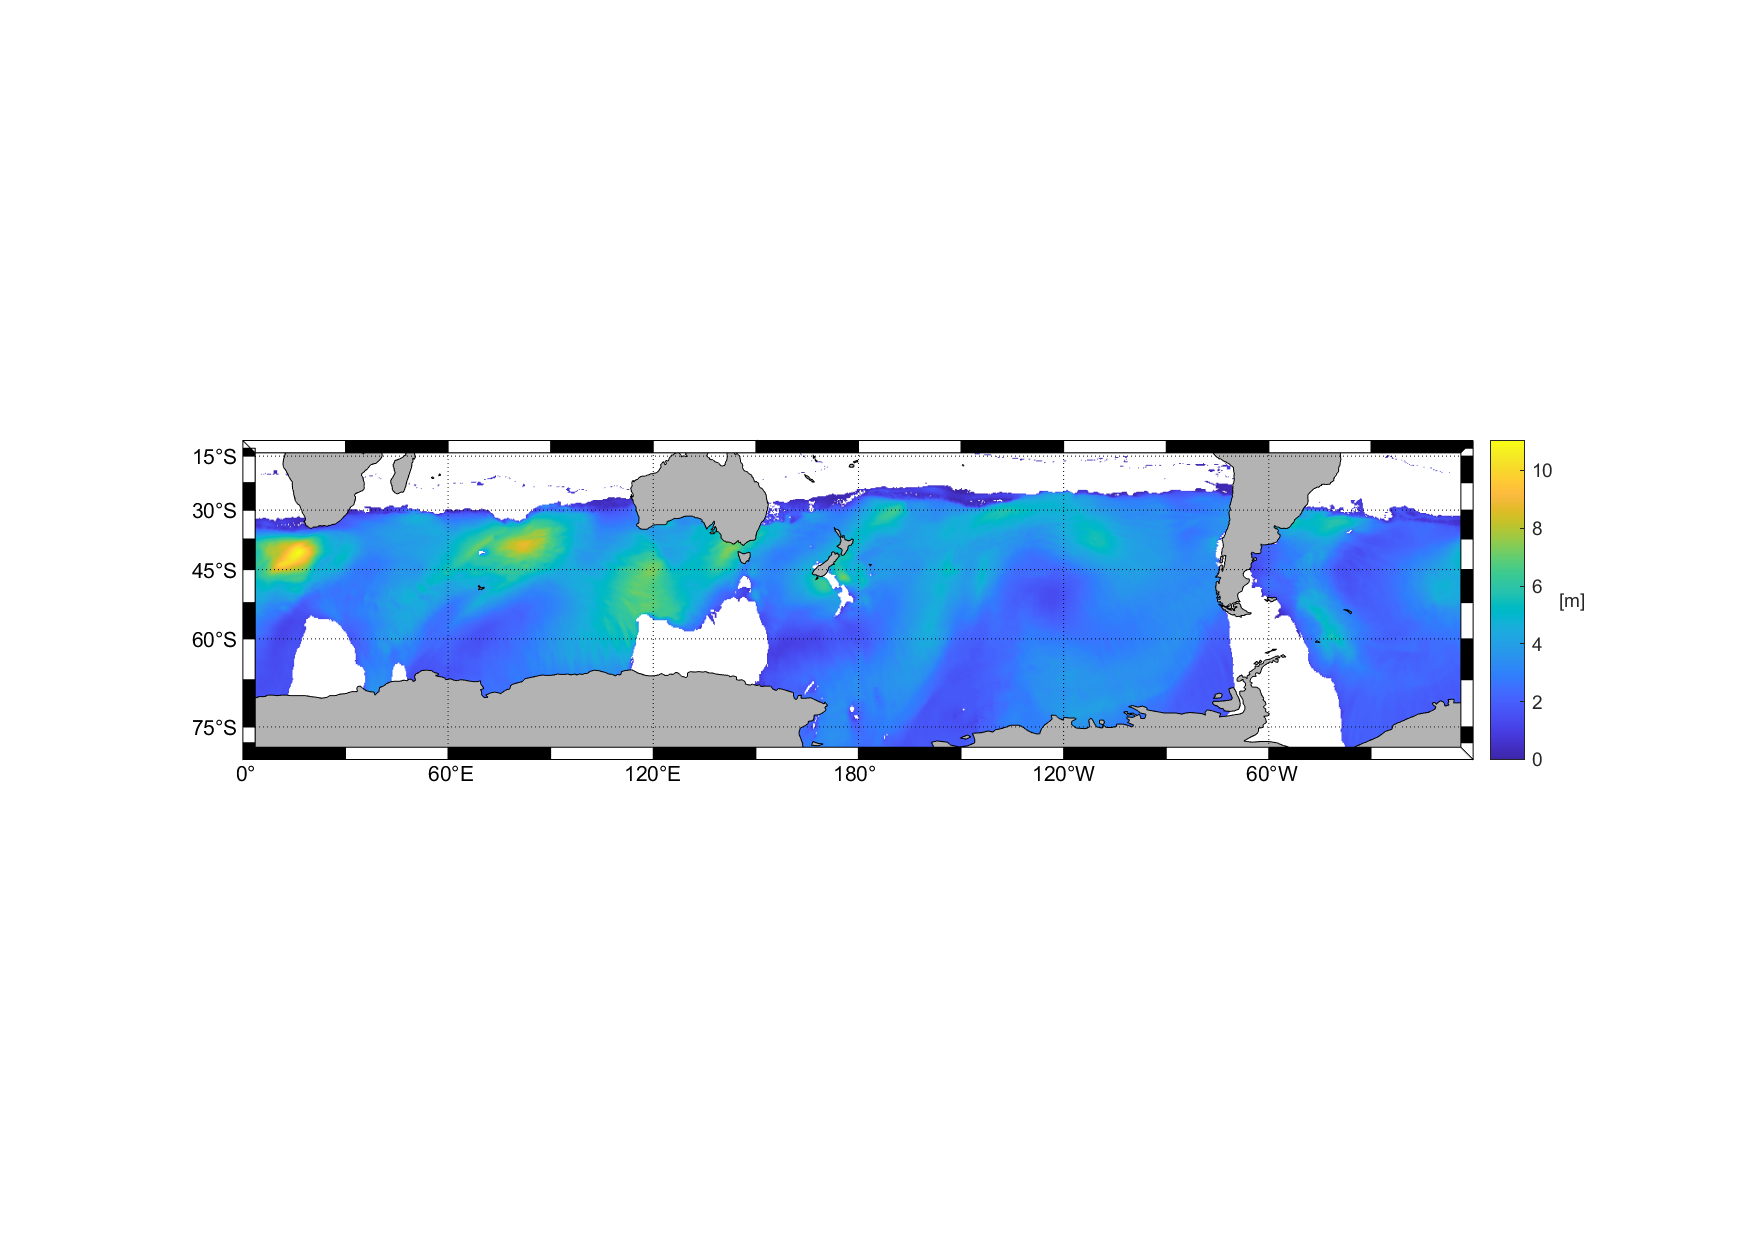
\includegraphics[width=\linewidth]{Figures/PipelineValidation/noaamillersignificantWaveHeight.pdf}
        \caption{Significant wave height.}
        \label{fig:pipelineVal.waveDataPlot.height}
    \end{subfigure}   
    \begin{subfigure}{0.48\linewidth}
        \centering
        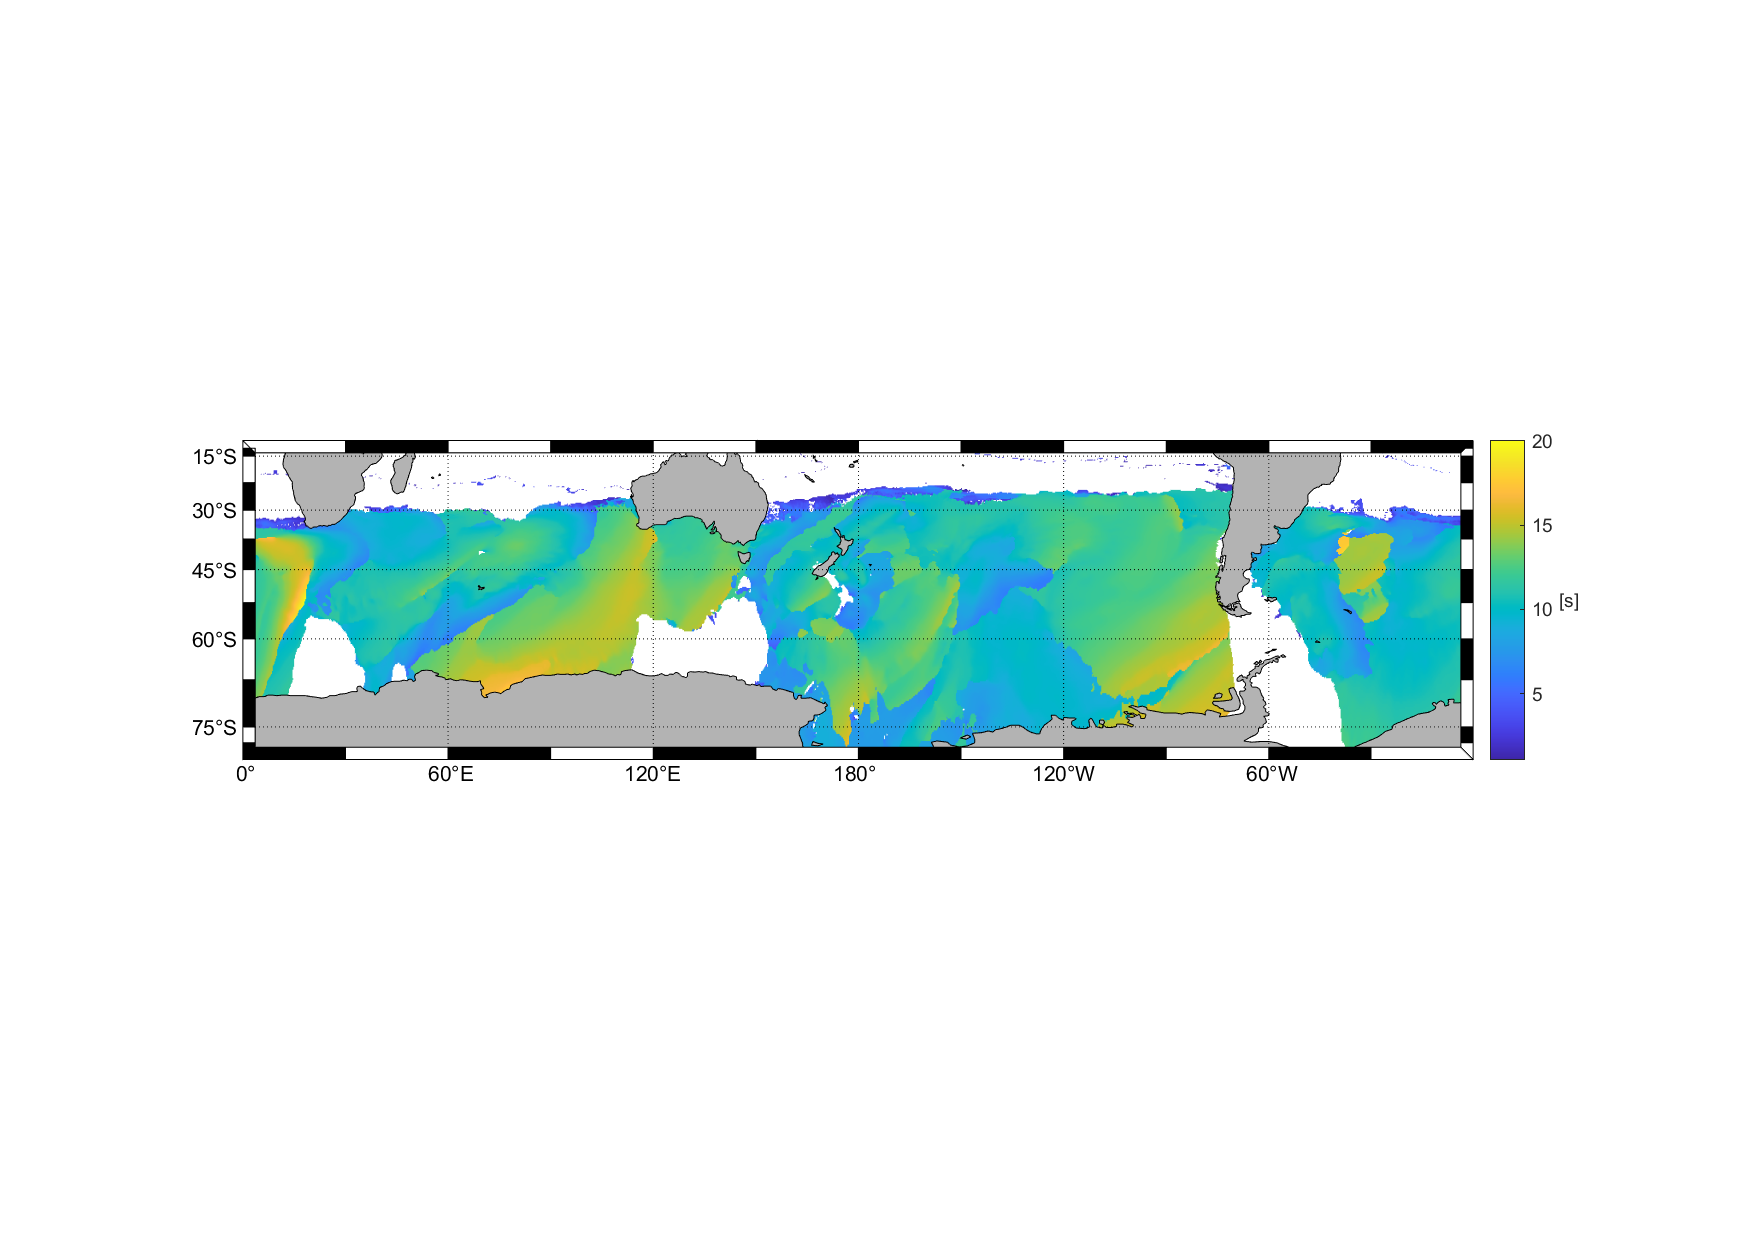
\includegraphics[width=\linewidth]{Figures/PipelineValidation/noaamillersignificantWavePeriod.pdf}
        \caption{Significant wave period.}
        \label{fig:pipelineVal.waveDataPlot.period}
    \end{subfigure}   
    \begin{subfigure}{0.48\linewidth}
        \centering
        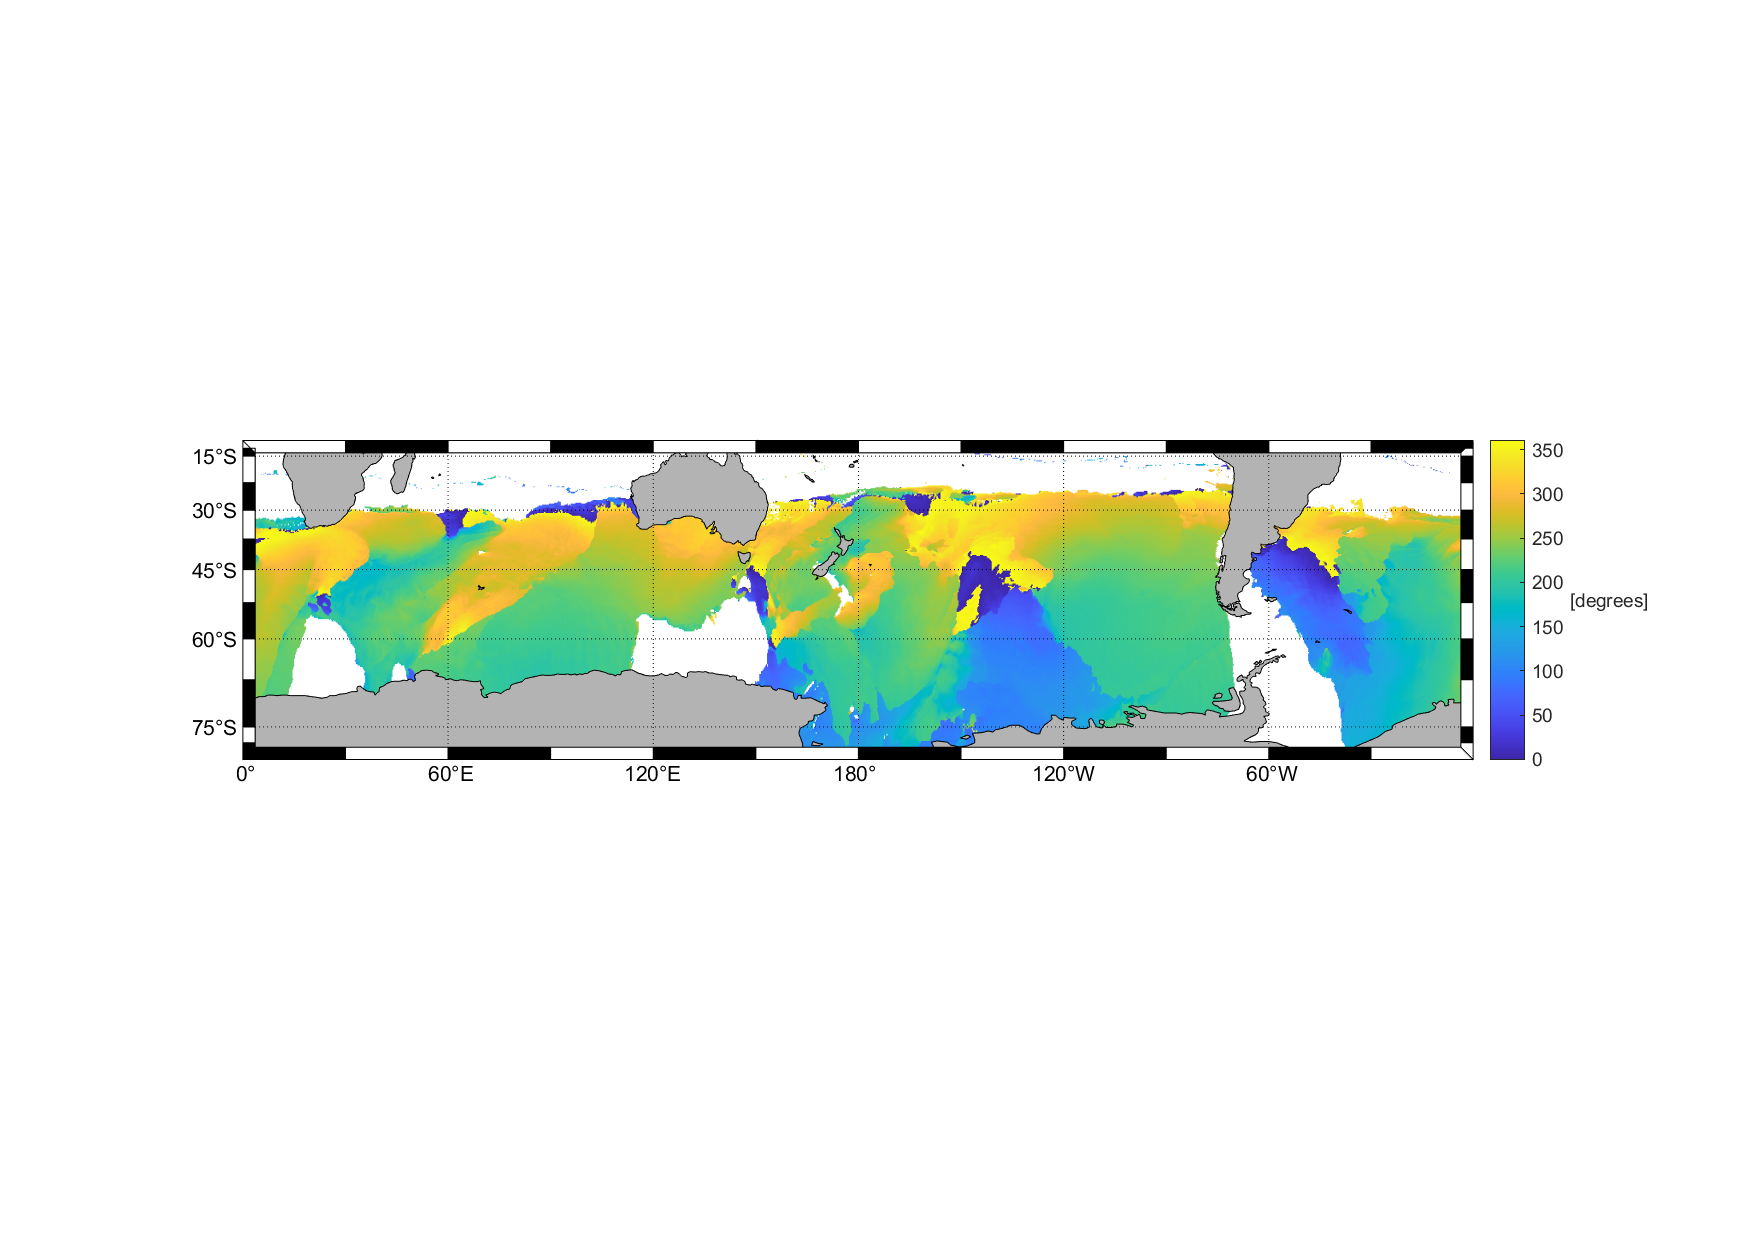
\includegraphics[width=\linewidth]{Figures/PipelineValidation/noaamillerdirection.pdf}
        \caption{Wave direction.}
        \label{fig:pipelineVal.waveDataPlot.direction}
    \end{subfigure}
    \begin{subfigure}{0.48\linewidth}
        \centering
        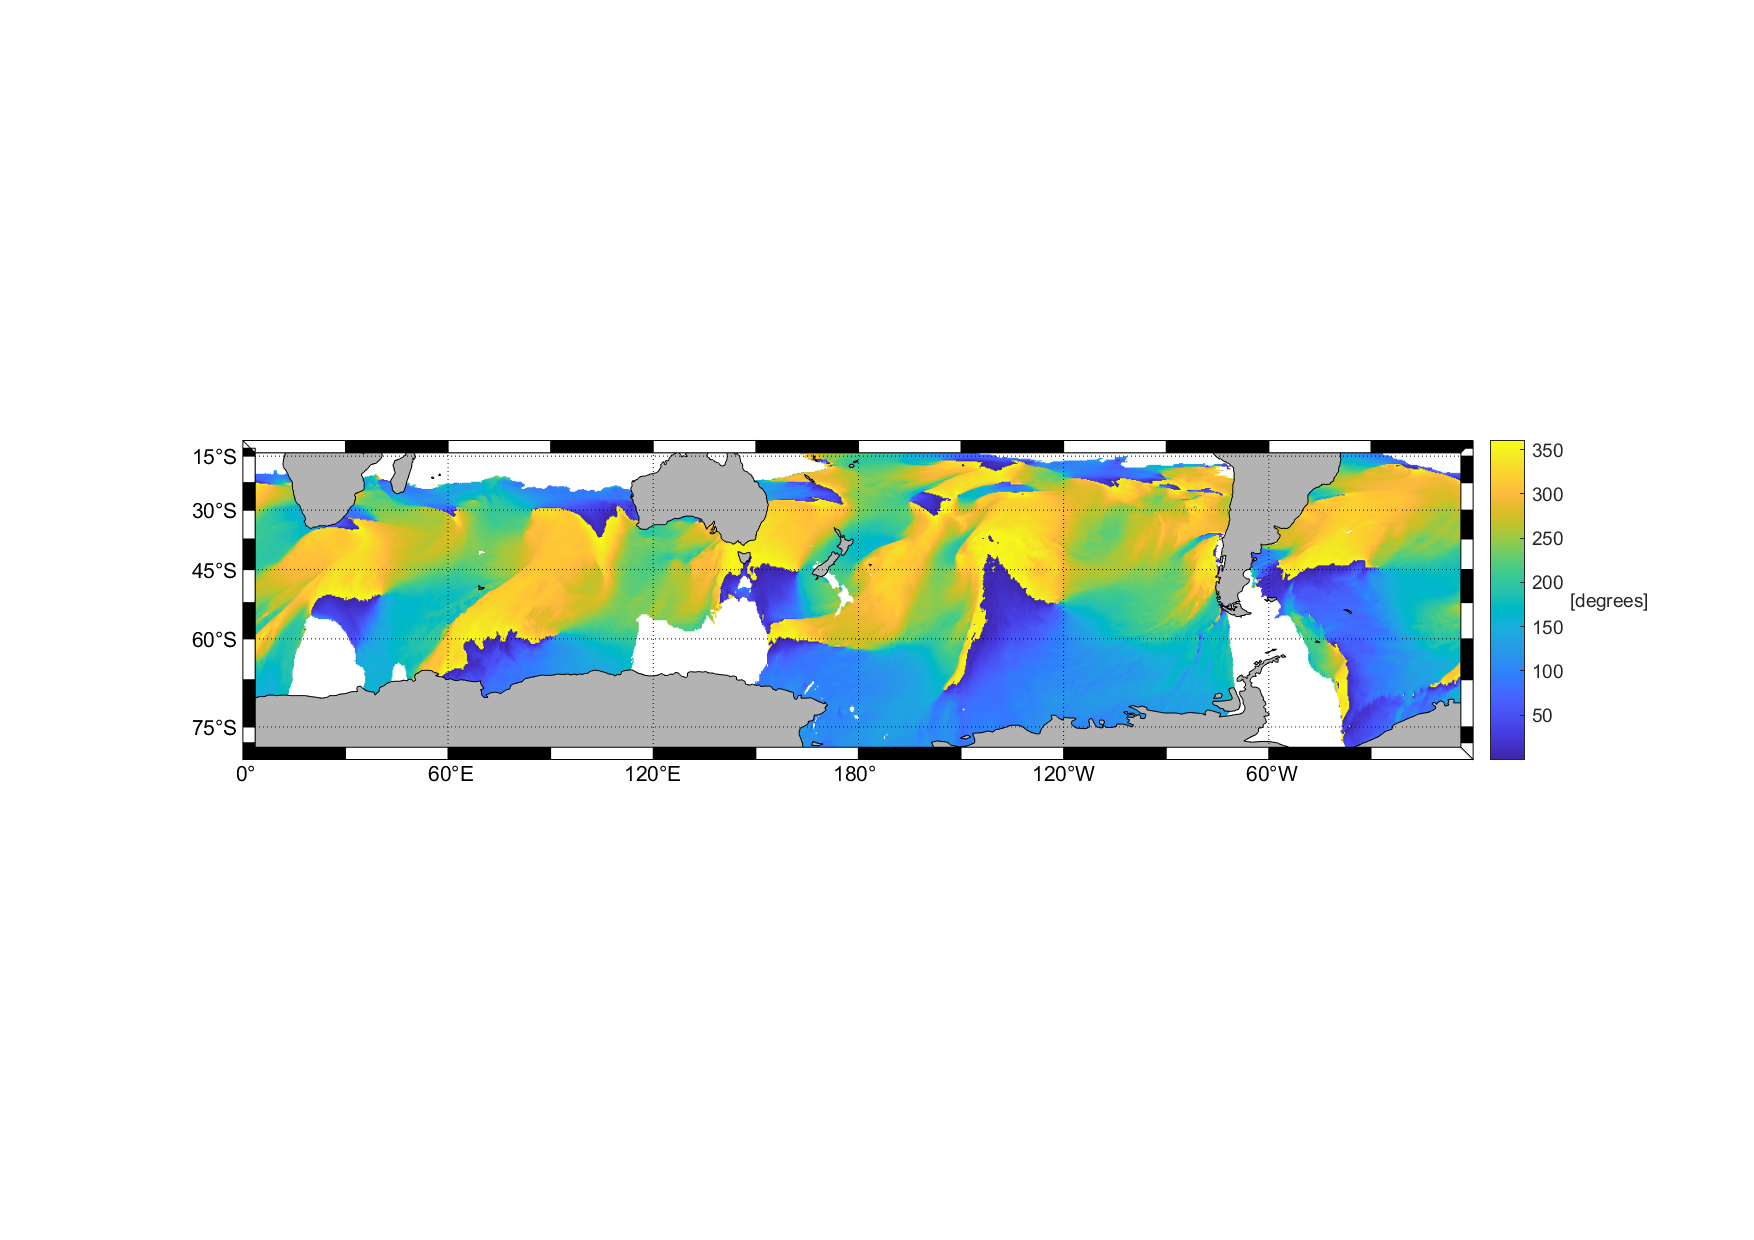
\includegraphics[width=\linewidth]{Figures/PipelineValidation/noaamillerwindDirection.pdf}
        \caption{Wind direction.}
        \label{fig:pipelineVal.waveDataPlot.windDirection}
    \end{subfigure}           
    \begin{subfigure}{0.48\linewidth}
        \centering
        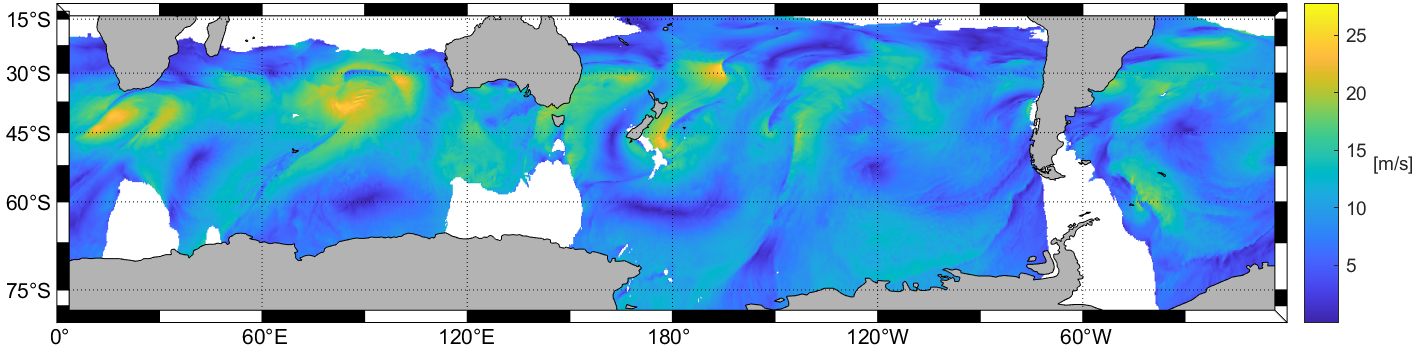
\includegraphics[width=\linewidth]{Figures/PipelineValidation/noaamillerwindSpeed.pdf}
        \caption{Wind speed.}
        \label{fig:pipelineVal.waveDataPlot.windSpeed}
    \end{subfigure}       
    \caption{M\_Map plots using Miller projection of various \acs{ncep} wave data parameters from 02-Oct-2023.}
    \label{fig:pipelineVal.waveDataPlot}
\end{figure}

Figures \ref{fig:pipelineVal.waveDataPlot.direction}, \ref{fig:pipelineVal.waveDataPlot.windDirection} both vary between 0 and 360$\degree$ which verifies that these data are correctly extracted. In terms of agreement within acceptable ranges for Figures \ref{fig:pipelineVal.waveDataPlot.height}, \ref{fig:pipelineVal.waveDataPlot.period}, \ref{fig:pipelineVal.waveDataPlot.windSpeed}, these range of these data makes sense. Therefore, the downloaded \acs{ncep} wave data, as well as both the \href{https://github.com/JNSRYA006/sar-parameter-extraction-pipeline/blob/main/functions/preprocess/get512Transects.m}{\lstinline{downloadNOAAWaveFile}} and \href{https://github.com/JNSRYA006/sar-parameter-extraction-pipeline/blob/main/functions/preprocess/get512Transects.m}{\lstinline{getGribStruct}} functions are implemented correctly.

\subsection{Wave Evolution} \label{subsec:pipelineVal.waveSpectra.waveEvolution}
%% Check holthuisjen expected changes are correct

In order to verify the way in which one-dimensional \acs{jonswap} wave spectra are constructed, it is essential to verify that the expected behaviour of waves when entering shallower water is met. As the depth of water decreases, the peak frequency of the wave is expected to decrease according to Equation \ref{eq:linearWaveTheory.dispersionRelationship.shallowWater}, as an increase in depth increases the $\omega_{peak}$ value. The height of the wave is expected to decrease due to the change in orbital motion of waves due to depth, as detailed in Chapter 5.4.2 of \cite{Holthuijsen2007}. 

To see these changes, geographic coordinates surrounding the Cape Point directional buoy were chosen. These coordinates were generated using the \href{https://github.com/JNSRYA006/sar-parameter-extraction-pipeline/blob/main/functions/waveSpectra/generateSingleJONSWAP.m}{\lstinline{createLatLonGrid}} function and the resulting coordinates are shown in Listing \ref{code:latLonExtract.grid}. However, due to the spatial resolution of 0.25$\degree$ provided by \acs{ncep} wave data, these points are not useful when validating the generation of the wave model. All of the individual points used to generate wave spectra are shown in Figure \ref{fig:pipelineVal.1DWaveSpectrum.map} along with the location of the \acs{csir} directional wave buoy. 

It is important to note that some points in Figure \ref{fig:pipelineVal.1DWaveSpectrum.map} do not aid the verification of generating accurate \acs{jonswap} spectra. The reasons why these are not suitable are discussed in Table \ref{tab:pipelineVal.1DWaveSpectrum.invalidLocs}.

\begin{table}[H]
\centering
\begin{tabular}{|c|c|c|}
\hline
\textbf{Figure \ref{fig:pipelineVal.1DWaveSpectrum.map} Label} & \textbf{Location ($\degree$)} & \textbf{Reason} \\ \hline
WS 1\_3(34S, 18.5E) & 34$\degree$\,S, 18.5$\degree$\,E & \begin{tabular}[c]{@{}c@{}}Data point located on land,\\ as opposed to the ocean.\end{tabular} \\ \hline
WS 2\_3(34.25S, 18.5E) & 34.25$\degree$\,S, 18.5$\degree$\,E & \begin{tabular}[c]{@{}c@{}}Data point located in  False Bay\\ (East of Cape Point), as opposed to being\\ West of Cape Point peninsula.\end{tabular} \\ \hline
WS 3\_3(34.5S, 18.5E) & 34.5$\degree$\,S, 18.5$\degree$\,E & No significant change in depth. \\ \hline
\end{tabular}
\caption{Data points generated by the \href{https://github.com/JNSRYA006/sar-parameter-extraction-pipeline/blob/main/functions/waveSpectra/generateSingleJONSWAP.m}{\lstinline{createLatLonGrid}} function not used to verify wave evolution over space.}
\label{tab:pipelineVal.1DWaveSpectrum.invalidLocs}
\end{table}


% Cite google earth pro and https://www.opendem.info/download_bathymetry.html
% Change labels to include lat and long
\begin{figure}[H]
    \centering
    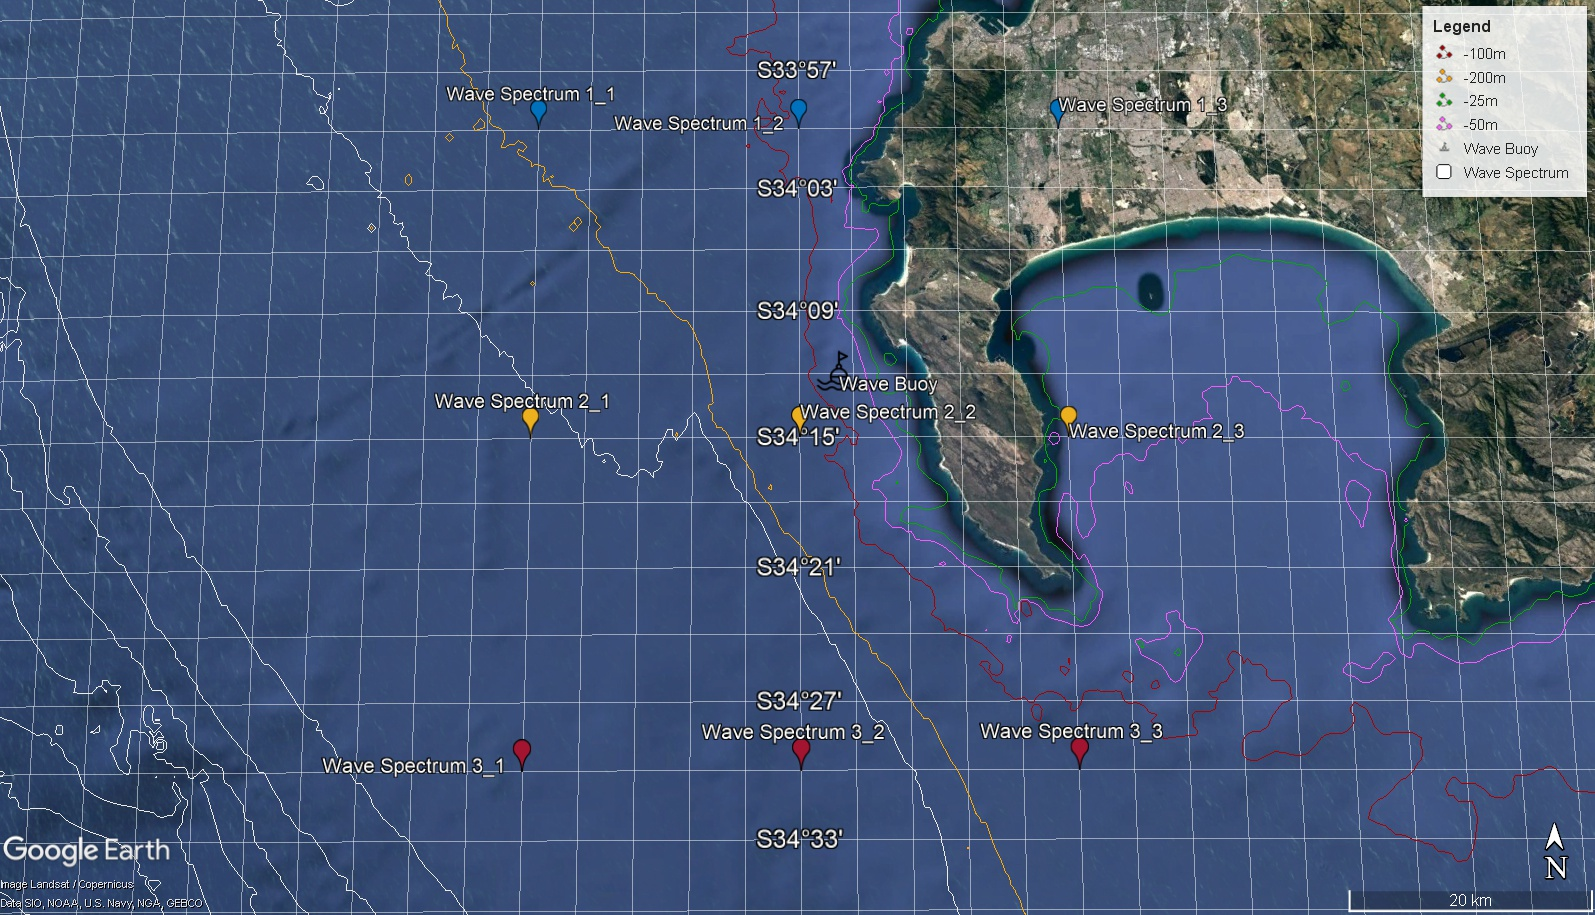
\includegraphics[width=.95\linewidth]{Figures/PipelineValidation/GoogleEarthWaveLocationsContoursGrid.pdf}
    \caption{Geographic points of generated \acs{jonswap} spectra using \acs{ncep} wave data. The location of the \acs{csir} directional wave buoy is shown. The points indicating each wave spectrum location correspond to the colours of the plots generated in Figure \ref{fig:pipelineVal.1DWaveSpectrum.all}. The contours shown in colour represent the respective depths below sea level: \textcolor{25m}{25\,m}, \textcolor{50m}{50\,m}, \textcolor{100m}{100\,m}, \textcolor{200m}{200\,m}, \textcolor{250m}{250\,m}, \textcolor{500m}{500\,m}, and \textcolor{750m}{750\,m}. Bathymetric contour data sourced and adapted from xx.}
    \label{fig:pipelineVal.1DWaveSpectrum.map}
\end{figure}

The wave spectra in Figure \ref{fig:pipelineVal.1DWaveSpectrum.all} can be seen to vary for different geographical locations. Examining each individual plot in Figures \ref{fig:pipelineVal.1DWaveSpectrum.1}, \ref{fig:pipelineVal.1DWaveSpectrum.2}, \ref{fig:pipelineVal.1DWaveSpectrum.3} allows the effect of change in depth to be determined, and verified.

\begin{figure}[H]
    \centering
    \subcaptionbox{\acs{jonswap} spectrum over three distinct latitudes and longitudes obtained from \acs{ncep} wave data. Wave spectra at the same latitude are shown in the same colour whilst the longitude of the wave spectra change.\label{fig:pipelineVal.1DWaveSpectrum.all}}[0.48\linewidth]{
        \resizebox{\linewidth}{!}{% This file was created by matlab2tikz.
%
%The latest updates can be retrieved from
%  http://www.mathworks.com/matlabcentral/fileexchange/22022-matlab2tikz-matlab2tikz
%where you can also make suggestions and rate matlab2tikz.
%
\definecolor{mycolor1}{rgb}{0.00000,0.44706,0.74118}%
\definecolor{mycolor2}{rgb}{0.92941,0.69412,0.12549}%
\definecolor{mycolor3}{rgb}{0.63529,0.07843,0.18431}%
%
\begin{tikzpicture}

\begin{axis}[%
width=4.521in,
height=3.524in,
at={(0.758in,0.523in)},
scale only axis,
unbounded coords=jump,
xmin=0,
xmax=7,
xtick={0,1.5707963267949,3.14159265358979,4.71238898038469,6.28318530717959},
xticklabels={{0},{$\pi\text{/2}$},{$\pi$},{$\text{3}\pi\text{/2}$},{$\text{2}\pi$}},
xlabel style={font=\color{white!15!black}},
xlabel={$\omega\text{ [rad/s]}$},
ymin=0,
ymax=0.07,
ylabel style={font=\color{white!15!black}},
ylabel={$\text{E(}\omega\text{) [m}^\text{2}\text{/rad/Hz]}$},
axis background/.style={fill=white},
axis x line*=bottom,
axis y line*=left,
xmajorgrids,
ymajorgrids,
legend style={legend cell align=left, align=left, draw=white!15!black}
]
\addplot [color=mycolor1]
  table[row sep=crcr]{%
0	nan\\
0.0122958616578857	0\\
0.0245917233157714	0\\
0.0368875849736571	0\\
0.0491834466315427	0\\
0.0614793082894284	0\\
0.0737751699473141	0\\
0.0860710316051998	0\\
0.0983668932630855	0\\
0.110662754920971	0\\
0.122958616578857	0\\
0.135254478236743	0\\
0.147550339894628	0\\
0.159846201552514	0\\
0.1721420632104	0\\
0.184437924868285	0\\
0.196733786526171	0\\
0.209029648184057	0\\
0.221325509841942	0\\
0.233621371499828	0\\
0.245917233157714	0\\
0.258213094815599	0\\
0.270508956473485	0\\
0.282804818131371	0\\
0.295100679789256	0\\
0.307396541447142	0\\
0.319692403105028	0\\
0.331988264762914	0\\
0.344284126420799	0\\
0.356579988078685	0\\
0.368875849736571	0\\
0.381171711394456	0\\
0.393467573052342	3.34419642251927e-289\\
0.405763434710228	1.28025550684515e-255\\
0.418059296368113	9.09801077678118e-227\\
0.430355158025999	7.17955661273785e-202\\
0.442651019683885	2.69655368843393e-180\\
0.45494688134177	1.58628012010437e-161\\
0.467242742999656	3.89542970829007e-145\\
0.479538604657542	8.98638404577865e-131\\
0.491834466315427	3.82270042312654e-118\\
0.504130327973313	5.26770583144193e-107\\
0.516426189631199	3.77319584880466e-97\\
0.528722051289085	2.09280440992325e-88\\
0.54101791294697	1.25940961397226e-80\\
0.553313774604856	1.09515982022289e-73\\
0.565609636262742	1.75705762280086e-67\\
0.577905497920627	6.41078704598093e-62\\
0.590201359578513	6.36556541298869e-57\\
0.602497221236399	2.00790222716586e-52\\
0.614793082894284	2.29975120115565e-48\\
0.62708894455217	1.0739089812567e-44\\
0.639384806210056	2.2611897369356e-41\\
0.651680667867941	2.34373434790845e-38\\
0.663976529525827	1.29120102064113e-35\\
0.676272391183713	4.04370246086255e-33\\
0.688568252841599	7.63655457505185e-31\\
0.700864114499484	9.16040465793229e-29\\
0.71315997615737	7.30704687792533e-27\\
0.725455837815256	4.03632650075498e-25\\
0.737751699473141	1.60048122856397e-23\\
0.750047561131027	4.70315840849396e-22\\
0.762343422788913	1.05373259129103e-20\\
0.774639284446798	1.84612768297031e-19\\
0.786935146104684	2.58700579350983e-18\\
0.79923100776257	2.95881393535563e-17\\
0.811526869420455	2.81249420426715e-16\\
0.823822731078341	2.25831112879919e-15\\
0.836118592736227	1.55434141155284e-14\\
0.848414454394112	9.29181663406122e-14\\
0.860710316051998	4.88210181401567e-13\\
0.873006177709884	2.27890731963973e-12\\
0.88530203936777	9.54283210921378e-12\\
0.897597901025655	3.61642202927237e-11\\
0.909893762683541	1.25025283956853e-10\\
0.922189624341426	3.97174755431221e-10\\
0.934485485999312	1.16706162830048e-09\\
0.946781347657198	3.19111067187954e-09\\
0.959077209315084	8.16400766983196e-09\\
0.971373070972969	1.9640330585374e-08\\
0.983668932630855	4.46335695515399e-08\\
0.995964794288741	9.62181033753792e-08\\
1.00826065594663	1.97513463595782e-07\\
1.02055651760451	3.87441107221251e-07\\
1.0328523792624	7.28589610711906e-07\\
1.04514824092028	1.31738947970889e-06\\
1.05744410257817	2.2965814013734e-06\\
1.06973996423605	3.86967598098188e-06\\
1.08203582589394	6.3167793390538e-06\\
1.09433168755183	1.00108401330565e-05\\
1.10662754920971	1.54331073387638e-05\\
1.1189234108676	2.31864186076149e-05\\
1.13121927252548	3.40048987204158e-05\\
1.14351513418337	4.8758751783582e-05\\
1.15581099584125	6.84530749027877e-05\\
1.16810685749914	9.4219982204407e-05\\
1.18040271915703	0.000127303769055645\\
1.19269858081491	0.000169039321722978\\
1.2049944424728	0.000220824440487555\\
1.21729030413068	0.000284087151892057\\
1.22958616578857	0.000360249404979067\\
1.24188202744645	0.000450688755701355\\
1.25417788910434	0.000556699734546854\\
1.26647375076223	0.000679456568201386\\
1.27876961242011	0.000819978800037321\\
1.291065474078	0.000979101146719596\\
1.30336133573588	0.00115744866365773\\
1.31565719739377	0.00135541799595638\\
1.32795305905165	0.00157316518818653\\
1.34024892070954	0.00181060023680969\\
1.35254478236743	0.00206738831012199\\
1.36484064402531	0.0023429573437477\\
1.3771365056832	0.0026365115513501\\
1.38943236734108	0.00294705027163909\\
1.40172822899897	0.00327339150067656\\
1.41402409065685	0.00361419942578141\\
1.42631995231474	0.00396801527386398\\
1.43861581397263	0.00433329080057555\\
1.45091167563051	0.00470842376409372\\
1.4632075372884	0.00509179473579552\\
1.47550339894628	0.00548180458817485\\
1.48779926060417	0.00587691195971112\\
1.50009512226205	0.00627566992269608\\
1.51239098391994	0.0066767609741115\\
1.52468684557783	0.00707902933805387\\
1.53698270723571	0.0074815094231008\\
1.5492785688936	0.00788344913644478\\
1.56157443055148	0.00828432663895199\\
1.57387029220937	0.00868385905314233\\
1.58616615386725	0.00908200162993884\\
1.59846201552514	0.00947893595725699\\
1.61075787718303	0.00987504596704363\\
1.62305373884091	0.0102708807757592\\
1.6353496004988	0.0106671037820176\\
1.64764546215668	0.0110644279490677\\
1.65994132381457	0.0114635378260619\\
1.67223718547245	0.0118649996213497\\
1.68453304713034	0.0122691615466052\\
1.69682890878822	0.0126760477126327\\
1.70912477044611	0.0130852500723398\\
1.721420632104	0.0134958242396934\\
1.73371649376188	0.0139061963823064\\
1.74601235541977	0.0143140896395624\\
1.75830821707765	0.0147164794313437\\
1.77060407873554	0.015109587298661\\
1.78289994039342	0.0154889222233254\\
1.79519580205131	0.0158493763991941\\
1.8074916637092	0.0161853789730349\\
1.81978752536708	0.016491106350086\\
1.83208338702497	0.0167607415774144\\
1.84437924868285	0.0169887687258095\\
1.85667511034074	0.0171702820380385\\
1.86897097199862	0.0173012850143819\\
1.88126683365651	0.0173789526276866\\
1.8935626953144	0.0174018877913857\\
1.90585855697228	0.0173792516945915\\
1.91815441863017	0.0173187030448506\\
1.93045028028805	0.0172218404888346\\
1.94274614194594	0.0170907927342484\\
1.95504200360382	0.0169281498507053\\
1.96733786526171	0.016736879485734\\
1.9796337269196	0.0165202329326319\\
1.99192958857748	0.0162816462986226\\
2.00422545023537	0.0160246419065975\\
2.01652131189325	0.0157527345731798\\
2.02881717355114	0.0154693466262642\\
2.04111303520902	0.015177734562442\\
2.05340889686691	0.0148809292085418\\
2.0657047585248	0.0145816902415667\\
2.07800062018268	0.0142824750172383\\
2.09029648184057	0.0139854209133983\\
2.10259234349845	0.0136923398385474\\
2.11488820515634	0.013404723192043\\
2.12718406681422	0.0131237553765477\\
2.13947992847211	0.012850333928277\\
2.15177579012999	0.012585094413024\\
2.16407165178788	0.0123284384010557\\
2.17636751344577	0.0120805630495126\\
2.18866337510365	0.0118414910596127\\
2.20095923676154	0.0116111000165573\\
2.21325509841942	0.0113891503476316\\
2.22555096007731	0.0111753113392689\\
2.2378468217352	0.0109691848321502\\
2.25014268339308	0.0107703263635373\\
2.26243854505097	0.0105782636491412\\
2.27473440670885	0.0103925123954185\\
2.28703026836674	0.0102125895103747\\
2.29932613002462	0.0100380238399035\\
2.31162199168251	0.00986836460031791\\
2.3239178533404	0.00970318770850608\\
2.33621371499828	0.00954210023112282\\
2.34850957665617	0.00938474318504906\\
2.36080543831405	0.00923079292435986\\
2.37310129997194	0.00907996134539838\\
2.38539716162982	0.00893199513229698\\
2.39769302328771	0.00878667425142768\\
2.40998888494559	0.0086438098857951\\
2.42228474660348	0.00850324198030174\\
2.43458060826137	0.0083648365470924\\
2.44687646991925	0.00822848285775266\\
2.45917233157714	0.00809409062684347\\
2.47146819323502	0.00796158726983848\\
2.48376405489291	0.00783091529859396\\
2.49605991655079	0.00770202989947307\\
2.50835577820868	0.00757489672346623\\
2.52065163986657	0.00744948990424842\\
2.53294750152445	0.00732579030911486\\
2.54524336318234	0.00720378401905237\\
2.55753922484022	0.00708346102766523\\
2.56983508649811	0.00696481414405219\\
2.58213094815599	0.0068478380817634\\
2.59442680981388	0.00673252871437512\\
2.60672267147177	0.00661888247773352\\
2.61901853312965	0.00650689589927961\\
2.63131439478754	0.00639656523584554\\
2.64361025644542	0.00628788620270682\\
2.65590611810331	0.00618085377832044\\
2.66820197976119	0.00607546207094004\\
2.68049784141908	0.0059717042350745\\
2.69279370307697	0.00586957242746926\\
2.70508956473485	0.0057690577938902\\
2.71738542639274	0.00567015047944444\\
2.72968128805062	0.00557283965646651\\
2.74197714970851	0.0054771135651265\\
2.75427301136639	0.00538295956288353\\
2.76656887302428	0.00529036417972385\\
2.77886473468217	0.00519931317680114\\
2.79116059634005	0.00510979160665305\\
2.80345645799794	0.00502178387361852\\
2.81575231965582	0.00493527379344081\\
2.82804818131371	0.0048502446513258\\
2.84034404297159	0.0047666792579471\\
2.85263990462948	0.00468456000306085\\
2.86493576628737	0.00460386890652315\\
2.87723162794525	0.00452458766660076\\
2.88952748960314	0.0044466977055378\\
2.90182335126102	0.00437018021239355\\
2.91411921291891	0.00429501618320338\\
2.92641507457679	0.00422118645854048\\
2.93871093623468	0.00414867175857284\\
2.95100679789256	0.00407745271572042\\
2.96330265955045	0.00400750990502326\\
2.97559852120834	0.00393882387233332\\
2.98789438286622	0.00387137516044325\\
3.00019024452411	0.00380514433326318\\
3.01248610618199	0.0037401119981539\\
3.02478196783988	0.00367625882652118\\
3.03707782949776	0.00361356557277201\\
3.04937369115565	0.00355201309172901\\
3.06166955281354	0.0034915823545951\\
3.07396541447142	0.00343225446355593\\
3.08626127612931	0.00337401066510325\\
3.09855713778719	0.00331683236215819\\
3.11085299944508	0.00326070112506917\\
3.12314886110296	0.00320559870155528\\
3.13544472276085	0.00315150702566218\\
3.14774058441874	0.00309840822579381\\
3.16003644607662	0.0030462846318797\\
3.17233230773451	0.00299511878173458\\
3.18462816939239	0.00294489342666344\\
3.19692403105028	0.00289559153636255\\
3.20921989270816	0.00284719630316386\\
3.22151575436605	0.00279969114566754\\
3.23381161602394	0.00275305971180489\\
3.24610747768182	0.00270728588137131\\
3.25840333933971	0.00266235376806688\\
3.27069920099759	0.00261824772107962\\
3.28299506265548	0.0025749523262447\\
3.29529092431336	0.00253245240681082\\
3.30758678597125	0.00249073302384293\\
3.31988264762914	0.00244977947628899\\
3.33217850928702	0.00240957730073666\\
3.34447437094491	0.00237011227088411\\
3.35677023260279	0.00233137039674796\\
3.36906609426068	0.0022933379236296\\
3.38136195591856	0.00225600133086013\\
3.39365781757645	0.00221934733034266\\
3.40595367923434	0.00218336286490959\\
3.41824954089222	0.00214803510651163\\
3.43054540255011	0.00211335145425364\\
3.44284126420799	0.00207929953229227\\
3.45513712586588	0.00204586718760842\\
3.46743298752376	0.00201304248766768\\
3.47972884918165	0.00198081371798019\\
3.49202471083954	0.00194916937957116\\
3.50432057249742	0.00191809818637236\\
3.51661643415531	0.00188758906254403\\
3.52891229581319	0.0018576311397364\\
3.54120815747108	0.00182821375429893\\
3.55350401912896	0.00179932644444514\\
3.56579988078685	0.00177095894738025\\
3.57809574244473	0.00174310119639827\\
3.59039160410262	0.00171574331795476\\
3.60268746576051	0.0016888756287211\\
3.61498332741839	0.00166248863262545\\
3.62727918907628	0.00163657301788557\\
3.63957505073416	0.00161111965403773\\
3.65187091239205	0.0015861195889663\\
3.66416677404994	0.00156156404593756\\
3.67646263570782	0.00153744442064151\\
3.68875849736571	0.00151375227824485\\
3.70105435902359	0.00149047935045825\\
3.71335022068148	0.00146761753262046\\
3.72564608233936	0.00144515888080198\\
3.73794194399725	0.00142309560893049\\
3.75023780565513	0.00140142008594007\\
3.76253366731302	0.00138012483294616\\
3.77482952897091	0.00135920252044798\\
3.78712539062879	0.00133864596555986\\
3.79942125228668	0.00131844812927288\\
3.81171711394456	0.00129860211374814\\
3.82401297560245	0.00127910115964251\\
3.83630883726033	0.00125993864346814\\
3.84860469891822	0.00124110807498621\\
3.86090056057611	0.00122260309463597\\
3.87319642223399	0.00120441747099944\\
3.88549228389188	0.00118654509830238\\
3.89778814554976	0.00116897999395205\\
3.91008400720765	0.00115171629611195\\
3.92237986886553	0.00113474826131388\\
3.93467573052342	0.00111807026210761\\
3.94697159218131	0.00110167678474807\\
3.95926745383919	0.00108556242692043\\
3.97156331549708	0.00106972189550273\\
3.98385917715496	0.00105415000436641\\
3.99615503881285	0.00103884167221433\\
4.00845090047073	0.00102379192045631\\
4.02074676212862	0.00100899587112205\\
4.03304262378651	0.000994448744811049\\
4.04533848544439	0.000980145858679543\\
4.05763434710228	0.000966082624463944\\
4.06993020876016	0.000952254546540628\\
4.08222607041805	0.000938657220021713\\
4.09452193207593	0.000925286328886466\\
4.10681779373382	0.00091213764414798\\
4.1191136553917	0.000899207022054753\\
4.13140951704959	0.000886490402326741\\
4.14370537870748	0.000873983806425488\\
4.15600124036536	0.000861683335857888\\
4.16829710202325	0.000849585170513158\\
4.18059296368113	0.000837685567032558\\
4.19288882533902	0.000825980857211403\\
4.2051846869969	0.0008144674464329\\
4.21748054865479	0.000803141812133341\\
4.22977641031268	0.000792000502298181\\
4.24207227197056	0.000781040133988504\\
4.25436813362845	0.000770257391897421\\
4.26666399528633	0.00075964902693588\\
4.27895985694422	0.000749211854847443\\
4.29125571860211	0.000738942754851508\\
4.30355158025999	0.000728838668314515\\
4.31584744191788	0.000718896597448629\\
4.32814330357576	0.000709113604037451\\
4.34043916523365	0.00069948680818823\\
4.35273502689153	0.000690013387110138\\
4.36503088854942	0.000680690573918113\\
4.37732675020731	0.000671515656461793\\
4.38962261186519	0.000662485976179102\\
4.40191847352308	0.000653598926973972\\
4.41421433518096	0.000644851954117806\\
4.42651019683885	0.000636242553174168\\
4.43880605849673	0.000627768268946294\\
4.45110192015462	0.000619426694446945\\
4.46339778181251	0.000611215469890196\\
4.47569364347039	0.000603132281704698\\
4.48798950512828	0.000595174861568003\\
4.50028536678616	0.000587340985461523\\
4.51258122844405	0.000579628472745707\\
4.52487709010193	0.000572035185255035\\
4.53717295175982	0.000564559026412404\\
4.5494688134177	0.000557197940362531\\
4.56176467507559	0.00054994991112397\\
4.57406053673348	0.000542812961759361\\
4.58635639839136	0.000535785153563524\\
4.59865226004925	0.000528864585269042\\
4.61094812170713	0.00052204939226895\\
4.62324398336502	0.000515337745856178\\
4.6355398450229	0.000508727852479397\\
4.64783570668079	0.000502217953014912\\
4.66013156833868	0.000495806322054271\\
4.67242742999656	0.000489491267207245\\
4.68472329165445	0.00048327112841986\\
4.69701915331233	0.000477144277307152\\
4.70931501497022	0.000471109116500332\\
4.7216108766281	0.000465164079008043\\
4.73390673828599	0.000459307627591423\\
4.74620259994388	0.000453538254152655\\
4.75849846160176	0.000447854479136719\\
4.77079432325965	0.000442254850946066\\
4.78309018491753	0.000436737945367922\\
4.79538604657542	0.000431302365013958\\
4.8076819082333	0.000425946738772039\\
4.81997776989119	0.000420669721269815\\
4.83227363154908	0.00041546999234986\\
4.84456949320696	0.00041034625655614\\
4.85686535486485	0.000405297242631535\\
4.86916121652273	0.000400321703026189\\
4.88145707818062	0.000395418413416441\\
4.8937529398385	0.000390586172234104\\
4.90604880149639	0.000385823800205873\\
4.91834466315427	0.000381130139902625\\
4.93064052481216	0.000376504055298402\\
4.94293638647005	0.000371944431338866\\
4.95523224812793	0.000367450173519001\\
4.96752810978582	0.000363020207469875\\
4.9798239714437	0.000358653478554253\\
4.99211983310159	0.000354348951470867\\
5.00441569475948	0.000350105609867147\\
5.01671155641736	0.000345922455960234\\
5.02900741807525	0.000341798510166082\\
5.04130327973313	0.000337732810736479\\
5.05359914139102	0.000333724413403804\\
5.0658950030489	0.000329772391033349\\
5.07819086470679	0.000325875833283049\\
5.09048672636467	0.000322033846270436\\
5.10278258802256	0.000318245552246677\\
5.11507844968045	0.000314510089277526\\
5.12737431133833	0.00031082661093104\\
5.13967017299622	0.000307194285971914\\
5.1519660346541	0.000303612298062282\\
5.16426189631199	0.000300079845468837\\
5.17655775796987	0.000296596140776148\\
5.18885361962776	0.000293160410606011\\
5.20114948128565	0.000289771895342729\\
5.21344534294353	0.000286429848864156\\
5.22574120460142	0.000283133538278418\\
5.2380370662593	0.000279882243666143\\
5.25033292791719	0.000276675257828116\\
5.26262878957507	0.000273511886038206\\
5.27492465123296	0.000270391445801484\\
5.28722051289085	0.000267313266617378\\
5.29951637454873	0.000264276689747787\\
5.31181223620662	0.000261281067990028\\
5.3241080978645	0.00025832576545451\\
5.33640395952239	0.000255410157347042\\
5.34869982118027	0.000252533629755657\\
5.36099568283816	0.000249695579441861\\
5.37329154449605	0.000246895413636219\\
5.38558740615393	0.00024413254983816\\
5.39788326781182	0.000241406415619933\\
5.4101791294697	0.000238716448434603\\
5.42247499112759	0.000236062095428015\\
5.43477085278547	0.000233442813254624\\
5.44706671444336	0.000230858067897119\\
5.45936257610125	0.00022830733448975\\
5.47165843775913	0.000225790097145283\\
5.48395429941702	0.000223305848785494\\
5.4962501610749	0.000220854090975143\\
5.50854602273279	0.000218434333759326\\
5.52084188439067	0.000216046095504163\\
5.53313774604856	0.000213688902740717\\
5.54543360770645	0.000211362290012102\\
5.55772946936433	0.000209065799723692\\
5.57002533102222	0.000206798981996369\\
5.5823211926801	0.000204561394522753\\
5.59461705433799	0.000202352602426333\\
5.60691291599587	0.000200172178123454\\
5.61920877765376	0.000198019701188079\\
5.63150463931164	0.000195894758219287\\
5.64380050096953	0.000193796942711433\\
5.65609636262742	0.000191725854926917\\
5.6683922242853	0.00018968110177151\\
5.68068808594319	0.000187662296672171\\
5.69298394760107	0.000185669059457322\\
5.70527980925896	0.000183701016239501\\
5.71757567091684	0.000181757799300367\\
5.72987153257473	0.000179839046977991\\
5.74216739423262	0.000177944403556393\\
5.7544632558905	0.000176073519157269\\
5.76675911754839	0.000174226049633875\\
5.77905497920627	0.000172401656466997\\
5.79135084086416	0.000170600006662997\\
5.80364670252204	0.000168820772653861\\
5.81594256417993	0.000167063632199222\\
5.82823842583782	0.000165328268290312\\
5.8405342874957	0.000163614369055801\\
5.85283014915359	0.000161921627669489\\
5.86512601081147	0.000160249742259805\\
5.87742187246936	0.000158598415821073\\
5.88971773412724	0.000156967356126522\\
5.90201359578513	0.000155356275642989\\
5.91430945744302	0.000153764891447277\\
5.9266053191009	0.000152192925144158\\
5.93890118075879	0.000150640102785949\\
5.95119704241667	0.000149106154793665\\
5.96349290407456	0.000147590815879686\\
5.97578876573244	0.000146093824971931\\
5.98808462739033	0.000144614925139487\\
6.00038048904822	0.000143153863519677\\
6.0126763507061	0.000141710391246535\\
6.02497221236399	0.000140284263380646\\
6.03726807402187	0.000138875238840341\\
6.04956393567976	0.000137483080334212\\
6.06185979733764	0.000136107554294908\\
6.07415565899553	0.000134748430814209\\
6.08645152065342	0.000133405483579327\\
6.0987473823113	0.000132078489810429\\
6.11104324396919	0.000130767230199341\\
6.12333910562707	0.000129471488849426\\
6.13563496728496	0.000128191053216586\\
6.14793082894284	0.0001269257140514\\
6.16022669060073	0.000125675265342338\\
6.17252255225862	0.000124439504260058\\
6.1848184139165	0.000123218231102752\\
6.19711427557439	0.000122011249242511\\
6.20941013723227	0.000120818365072709\\
6.22170599889016	0.000119639387956367\\
6.23400186054804	0.000118474130175486\\
6.24629772220593	0.000117322406881326\\
6.25859358386381	0.000116184036045615\\
6.2708894455217	0.000115058838412668\\
6.28318530717959	0.000113946637452394\\
};
\addlegendentry{-34S, 18E}

\addplot [color=mycolor1]
  table[row sep=crcr]{%
0	nan\\
0.0122958616578857	0\\
0.0245917233157714	0\\
0.0368875849736571	0\\
0.0491834466315427	0\\
0.0614793082894284	0\\
0.0737751699473141	0\\
0.0860710316051998	0\\
0.0983668932630855	0\\
0.110662754920971	0\\
0.122958616578857	0\\
0.135254478236743	0\\
0.147550339894628	0\\
0.159846201552514	0\\
0.1721420632104	0\\
0.184437924868285	0\\
0.196733786526171	0\\
0.209029648184057	0\\
0.221325509841942	0\\
0.233621371499828	0\\
0.245917233157714	0\\
0.258213094815599	0\\
0.270508956473485	0\\
0.282804818131371	0\\
0.295100679789256	0\\
0.307396541447142	0\\
0.319692403105028	0\\
0.331988264762914	0\\
0.344284126420799	0\\
0.356579988078685	0\\
0.368875849736571	0\\
0.381171711394456	0\\
0.393467573052342	0\\
0.405763434710228	0\\
0.418059296368113	0\\
0.430355158025999	0\\
0.442651019683885	0\\
0.45494688134177	0\\
0.467242742999656	0\\
0.479538604657542	1.5177491991091e-304\\
0.491834466315427	3.59988792837343e-275\\
0.504130327973313	2.97459350772964e-249\\
0.516426189631199	2.56579944919526e-226\\
0.528722051289085	5.82620337498939e-206\\
0.54101791294697	7.61878290228262e-188\\
0.553313774604856	1.11573250221128e-171\\
0.565609636262742	3.22639479339998e-157\\
0.577905497920627	2.99326558863239e-144\\
0.590201359578513	1.35158996643375e-132\\
0.602497221236399	4.25350312235513e-122\\
0.614793082894284	1.27233209270532e-112\\
0.62708894455217	4.7336973099415e-104\\
0.639384806210056	2.76737767955296e-96\\
0.651680667867941	3.11668922805648e-89\\
0.663976529525827	8.07996656146955e-83\\
0.676272391183713	5.63603459066287e-77\\
0.688568252841599	1.21310249989219e-71\\
0.700864114499484	9.09022062801702e-67\\
0.71315997615737	2.63776355661956e-62\\
0.725455837815256	3.25660969564585e-58\\
0.737751699473141	1.85949738629826e-54\\
0.750047561131027	5.28810364461862e-51\\
0.762343422788913	8.00031674502866e-48\\
0.774639284446798	6.82871515386742e-45\\
0.786935146104684	3.46569129663185e-42\\
0.79923100776257	1.09611209455118e-39\\
0.811526869420455	2.25327592914055e-37\\
0.823822731078341	3.1266557871064e-35\\
0.836118592736227	3.0297784779839e-33\\
0.848414454394112	2.11397572544735e-31\\
0.860710316051998	1.09178964025164e-29\\
0.873006177709884	4.27918697034194e-28\\
0.88530203936777	1.30187203096018e-26\\
0.897597901025655	3.13790831844393e-25\\
0.909893762683541	6.10426895616376e-24\\
0.922189624341426	9.74692322018436e-23\\
0.934485485999312	1.2971778572717e-21\\
0.946781347657198	1.45912746508214e-20\\
0.959077209315084	1.40500562520106e-19\\
0.971373070972969	1.17166183958563e-18\\
0.983668932630855	8.55224747752652e-18\\
0.995964794288741	5.51740059672603e-17\\
1.00826065594663	3.17419282717501e-16\\
1.02055651760451	1.64181467054088e-15\\
1.0328523792624	7.69243398971522e-15\\
1.04514824092028	3.28734431545025e-14\\
1.05744410257817	1.28950082606121e-13\\
1.06973996423605	4.67012259083545e-13\\
1.08203582589394	1.57000789586639e-12\\
1.09433168755183	4.9237725428578e-12\\
1.10662754920971	1.44712902639738e-11\\
1.1189234108676	4.00285009076741e-11\\
1.13121927252548	1.04613062471867e-10\\
1.14351513418337	2.59258185621193e-10\\
1.15581099584125	6.11320242789879e-10\\
1.16810685749914	1.3757784151925e-09\\
1.18040271915703	2.96365685301422e-09\\
1.19269858081491	6.12736688043932e-09\\
1.2049944424728	1.21890807680256e-08\\
1.21729030413068	2.33844937993752e-08\\
1.22958616578857	4.33594777350743e-08\\
1.24188202744645	7.78599228564314e-08\\
1.25417788910434	1.35654197810242e-07\\
1.26647375076223	2.29721982474434e-07\\
1.27876961242011	3.78732009005106e-07\\
1.291065474078	6.08814350833128e-07\\
1.30336133573588	9.55610939896489e-07\\
1.31565719739377	1.46656234099676e-06\\
1.32795305905165	2.20336150144649e-06\\
1.34024892070954	3.24447870746303e-06\\
1.35254478236743	4.68763896346173e-06\\
1.36484064402531	6.65211595958453e-06\\
1.3771365056832	9.2806977441807e-06\\
1.38943236734108	1.27411795137341e-05\\
1.40172822899897	1.72272490712665e-05\\
1.41402409065685	2.29586500980031e-05\\
1.42631995231474	3.01805362204644e-05\\
1.43861581397263	3.91619630494999e-05\\
1.45091167563051	5.01935035672044e-05\\
1.4632075372884	6.35840118648192e-05\\
1.47550339894628	7.96565987261822e-05\\
1.48779926060417	9.8743917571007e-05\\
1.50009512226205	0.000121182888880167\\
1.51239098391994	0.000147309013990663\\
1.52468684557783	0.000177450444205305\\
1.53698270723571	0.000211921978211975\\
1.5492785688936	0.000251019160072167\\
1.56157443055148	0.000295012642184872\\
1.57387029220937	0.000344142963670265\\
1.58616615386725	0.000398615875793367\\
1.59846201552514	0.000458598323731767\\
1.61075787718303	0.00052421516958042\\
1.62305373884091	0.000595546716316724\\
1.6353496004988	0.000672627067727991\\
1.64764546215668	0.000755443336059002\\
1.65994132381457	0.000843935688185586\\
1.67223718547245	0.000937998203047975\\
1.68453304713034	0.00103748049823957\\
1.69682890878822	0.00114219007217248\\
1.70912477044611	0.00125189530005069\\
1.721420632104	0.00136632901670872\\
1.73371649376188	0.00148519261679078\\
1.74601235541977	0.00160816060219696\\
1.75830821707765	0.00173488550755875\\
1.77060407873554	0.00186500313601892\\
1.78289994039342	0.00199813803905882\\
1.79519580205131	0.00213390917484883\\
1.8074916637092	0.00227193567897818\\
1.81978752536708	0.0024118426789608\\
1.83208338702497	0.00255326707929256\\
1.84437924868285	0.00269586323694338\\
1.85667511034074	0.00283930843813629\\
1.86897097199862	0.00298330807647963\\
1.88126683365651	0.00312760042061802\\
1.8935626953144	0.00327196084741591\\
1.90585855697228	0.00341620540532807\\
1.91815441863017	0.00356019356319949\\
1.93045028028805	0.00370382999345466\\
1.94274614194594	0.00384706523661276\\
1.95504200360382	0.00398989509729419\\
1.96733786526171	0.00413235863117173\\
1.9796337269196	0.00427453459826196\\
1.99192958857748	0.00441653628095377\\
2.00422545023537	0.00455850459550551\\
2.01652131189325	0.00470059946364676\\
2.02881717355114	0.0048429894567002\\
2.04111303520902	0.00498583977875313\\
2.05340889686691	0.00512929871850011\\
2.0657047585248	0.00527348277220985\\
2.07800062018268	0.00541846072351415\\
2.09029648184057	0.00556423705959786\\
2.10259234349845	0.00571073520713288\\
2.11488820515634	0.0058577811825584\\
2.12718406681422	0.00600508836532656\\
2.13947992847211	0.00615224421177293\\
2.15177579012999	0.00629869982017911\\
2.16407165178788	0.00644376331981627\\
2.17636751344577	0.00658659807099042\\
2.18866337510365	0.00672622661078132\\
2.20095923676154	0.00686154114278783\\
2.21325509841942	0.00699132113552472\\
2.22555096007731	0.00711425825782542\\
2.2378468217352	0.00722898844686448\\
2.25014268339308	0.00733413039569875\\
2.26243854505097	0.00742832919843569\\
2.27473440670885	0.00751030335226276\\
2.28703026836674	0.0075788928464522\\
2.29932613002462	0.00763310573169314\\
2.31162199168251	0.00767216041489473\\
2.3239178533404	0.00769552100493388\\
2.33621371499828	0.00770292655256459\\
2.34850957665617	0.00769686708816549\\
2.36080543831405	0.0076796973960154\\
2.37310129997194	0.00765174912698079\\
2.38539716162982	0.00761345986184636\\
2.39769302328771	0.00756536395588909\\
2.40998888494559	0.00750808114182649\\
2.42228474660348	0.00744230334630768\\
2.43458060826137	0.00736878023015177\\
2.44687646991925	0.00728830398822063\\
2.45917233157714	0.00720169394146257\\
2.47146819323502	0.00710978142370521\\
2.48376405489291	0.00701339541335335\\
2.49605991655079	0.00691334929060336\\
2.50835577820868	0.00681042902008442\\
2.52065163986657	0.00670538297299621\\
2.53294750152445	0.0065989135174123\\
2.54524336318234	0.00649167042521316\\
2.55753922484022	0.00638424607278976\\
2.56983508649811	0.00627717235272493\\
2.58213094815599	0.00617091916646098\\
2.59442680981388	0.00606589433379059\\
2.60672267147177	0.00596244473329087\\
2.61901853312965	0.00586085847732994\\
2.63131439478754	0.00576136792435896\\
2.64361025644542	0.00566415333798879\\
2.65590611810331	0.00556934701493151\\
2.66820197976119	0.00547703772045325\\
2.68049784141908	0.00538727528892769\\
2.69279370307697	0.00530007526704495\\
2.70508956473485	0.0052154234971452\\
2.71738542639274	0.00513328055721164\\
2.72968128805062	0.00505358599172931\\
2.74197714970851	0.00497626228356617\\
2.75427301136639	0.00490121853110981\\
2.76656887302428	0.00482835380707803\\
2.77886473468217	0.0047575601857907\\
2.79116059634005	0.00468872543437854\\
2.80345645799794	0.0046217353705768\\
2.81575231965582	0.00455647589558584\\
2.82804818131371	0.00449283471514409\\
2.84034404297159	0.00443070276560932\\
2.85263990462948	0.00436997536461688\\
2.86493576628737	0.00431055310789405\\
2.87723162794525	0.00425234253515672\\
2.88952748960314	0.00419525658877825\\
2.90182335126102	0.00413921488917146\\
2.91411921291891	0.0040841438506249\\
2.92641507457679	0.00402997666074001\\
2.93871093623468	0.0039766531456817\\
2.95100679789256	0.00392411954223473\\
2.96330265955045	0.00387232819620575\\
2.97559852120834	0.00382123720507953\\
2.98789438286622	0.00377081002108193\\
3.00019024452411	0.00372101502897119\\
3.01248610618199	0.00367182511102408\\
3.02478196783988	0.00362321720984694\\
3.03707782949776	0.00357517189786452\\
3.04937369115565	0.00352767296065455\\
3.06166955281354	0.00348070699973007\\
3.07396541447142	0.0034342630589452\\
3.08626127612931	0.00338833227742614\\
3.09855713778719	0.00334290757081521\\
3.11085299944508	0.00329798334166302\\
3.12314886110296	0.00325355521900883\\
3.13544472276085	0.00320961982654435\\
3.14774058441874	0.00316617457825077\\
3.16003644607662	0.00312321750002014\\
3.17233230773451	0.00308074707550543\\
3.18462816939239	0.00303876211427411\\
3.19692403105028	0.00299726164025308\\
3.20921989270816	0.00295624479843271\\
3.22151575436605	0.00291571077783244\\
3.23381161602394	0.00287565874880613\\
3.24610747768182	0.00283608781287189\\
3.25840333933971	0.00279699696337842\\
3.27069920099759	0.00275838505546025\\
3.28299506265548	0.00272025078387996\\
3.29529092431336	0.00268259266750304\\
3.30758678597125	0.0026454090392936\\
3.31988264762914	0.00260869804085671\\
3.33217850928702	0.00257245762068047\\
3.34447437094491	0.00253668553534947\\
3.35677023260279	0.00250137935310764\\
3.36906609426068	0.00246653645924508\\
3.38136195591856	0.00243215406286795\\
3.39365781757645	0.00239822920468509\\
3.40595367923434	0.00236475876550993\\
3.41824954089222	0.00233173947523137\\
3.43054540255011	0.00229916792205502\\
3.44284126420799	0.00226704056185601\\
3.45513712586588	0.00223535372751809\\
3.46743298752376	0.00220410363816165\\
3.47972884918165	0.00217328640818613\\
3.49202471083954	0.00214289805607133\\
3.50432057249742	0.00211293451289692\\
3.51661643415531	0.00208339163055214\\
3.52891229581319	0.00205426518961718\\
3.54120815747108	0.0020255509069055\\
3.55350401912896	0.00199724444266243\\
3.56579988078685	0.00196934140742003\\
3.57809574244473	0.00194183736851154\\
3.59039160410262	0.00191472785625186\\
3.60268746576051	0.00188800836979189\\
3.61498332741839	0.00186167438265634\\
3.62727918907628	0.00183572134797542\\
3.63957505073416	0.00181014470342146\\
3.65187091239205	0.00178493987586171\\
3.66416677404994	0.00176010228573899\\
3.67646263570782	0.00173562735119154\\
3.68875849736571	0.00171151049192352\\
3.70105435902359	0.00168774713283716\\
3.71335022068148	0.00166433270743775\\
3.72564608233936	0.00164126266102156\\
3.73794194399725	0.00161853245365746\\
3.75023780565513	0.00159613756297164\\
3.76253366731302	0.00157407348674526\\
3.77482952897091	0.00155233574533408\\
3.78712539062879	0.00153091988391876\\
3.79942125228668	0.00150982147459445\\
3.81171711394456	0.00148903611830757\\
3.82401297560245	0.00146855944664759\\
3.83630883726033	0.00144838712350126\\
3.84860469891822	0.00142851484657624\\
3.86090056057611	0.00140893834880102\\
3.87319642223399	0.00138965339960752\\
3.88549228389188	0.00137065580610259\\
3.89778814554976	0.00135194141413426\\
3.91008400720765	0.00133350610925843\\
3.92237986886553	0.00131534581761133\\
3.93467573052342	0.00129745650669287\\
3.94697159218131	0.00127983418606577\\
3.95926745383919	0.00126247490797524\\
3.97156331549708	0.0012453747678934\\
3.98385917715496	0.00122852990499295\\
3.99615503881285	0.001211936502554\\
4.00845090047073	0.0011955907883078\\
4.02074676212862	0.0011794890347213\\
4.03304262378651	0.00116362755922569\\
4.04533848544439	0.00114800272439253\\
4.05763434710228	0.00113261093806047\\
4.06993020876016	0.00111744865341553\\
4.08222607041805	0.00110251236902794\\
4.09452193207593	0.00108779862884813\\
4.10681779373382	0.0010733040221645\\
4.1191136553917	0.00105902518352541\\
4.13140951704959	0.00104495879262773\\
4.14370537870748	0.00103110157417414\\
4.15600124036536	0.00101745029770131\\
4.16829710202325	0.00100400177738097\\
4.18059296368113	0.000990752871795653\\
4.19288882533902	0.000977700483691099\\
4.2051846869969	0.000964841559706807\\
4.21748054865479	0.000952173090086521\\
4.22977641031268	0.000939692108370099\\
4.24207227197056	0.000927395691068213\\
4.25436813362845	0.000915280957321297\\
4.26666399528633	0.000903345068543989\\
4.27895985694422	0.000891585228056354\\
4.29125571860211	0.000879998680702995\\
4.30355158025999	0.000868582712461209\\
4.31584744191788	0.000857334650039176\\
4.32814330357576	0.000846251860465213\\
4.34043916523365	0.000835331750668981\\
4.35273502689153	0.000824571767055553\\
4.36503088854942	0.000813969395073145\\
4.37732675020731	0.000803522158775313\\
4.38962261186519	0.00079322762037834\\
4.40191847352308	0.000783083379814493\\
4.41421433518096	0.000773087074281842\\
4.42651019683885	0.000763236377791201\\
4.43880605849673	0.00075352900071082\\
4.45110192015462	0.000743962689309325\\
4.46339778181251	0.000734535225297458\\
4.47569364347039	0.000725244425369058\\
4.48798950512828	0.000716088140741748\\
4.50028536678616	0.000707064256697753\\
4.51258122844405	0.000698170692125227\\
4.52487709010193	0.000689405399060467\\
4.53717295175982	0.000680766362231351\\
4.5494688134177	0.000672251598602318\\
4.56176467507559	0.000663859156921196\\
4.57406053673348	0.000655587117268152\\
4.58635639839136	0.000647433590607007\\
4.59865226004925	0.000639396718339181\\
4.61094812170713	0.00063147467186047\\
4.62324398336502	0.000623665652120859\\
4.6355398450229	0.000615967889187574\\
4.64783570668079	0.000608379641811531\\
4.66013156833868	0.000600899196997353\\
4.67242742999656	0.000593524869577093\\
4.68472329165445	0.000586255001787801\\
4.69701915331233	0.000579087962853049\\
4.70931501497022	0.000572022148568545\\
4.7216108766281	0.000565055980891898\\
4.73390673828599	0.000558187907536667\\
4.74620259994388	0.000551416401570736\\
4.75849846160176	0.000544739961019108\\
4.77079432325965	0.000538157108471181\\
4.78309018491753	0.000531666390692533\\
4.79538604657542	0.000525266378241307\\
4.8076819082333	0.000518955665089195\\
4.81997776989119	0.000512732868247075\\
4.83227363154908	0.000506596627395324\\
4.84456949320696	0.000500545604518827\\
4.85686535486485	0.000494578483546695\\
4.86916121652273	0.000488693969996709\\
4.88145707818062	0.000482890790624483\\
4.8937529398385	0.00047716769307736\\
4.90604880149639	0.000471523445553034\\
4.91834466315427	0.000465956836462878\\
4.93064052481216	0.000460466674099991\\
4.94293638647005	0.00045505178631192\\
4.95523224812793	0.00044971102017807\\
4.96752810978582	0.000444443241691753\\
4.9798239714437	0.000439247335446869\\
4.99211983310159	0.000434122204329193\\
5.00441569475948	0.000429066769212227\\
5.01671155641736	0.0004240799686576\\
5.02900741807525	0.000419160758619969\\
5.04130327973313	0.00041430811215641\\
5.05359914139102	0.000409521019140223\\
5.0658950030489	0.00040479848597916\\
5.07819086470679	0.000400139535337993\\
5.09048672636467	0.000395543205865417\\
5.10278258802256	0.000391008551925216\\
5.11507844968045	0.000386534643331674\\
5.12737431133833	0.000382120565089164\\
5.13967017299622	0.000377765417135891\\
5.1519660346541	0.000373468314091729\\
5.16426189631199	0.000369228385010106\\
5.17655775796987	0.000365044773133905\\
5.18885361962776	0.000360916635655306\\
5.20114948128565	0.000356843143479556\\
5.21344534294353	0.000352823480992579\\
5.22574120460142	0.000348856845832419\\
5.2380370662593	0.000344942448664427\\
5.25033292791719	0.000341079512960177\\
5.26262878957507	0.000337267274780035\\
5.27492465123296	0.000333504982559352\\
5.28722051289085	0.000329791896898218\\
5.29951637454873	0.000326127290354734\\
5.31181223620662	0.000322510447241752\\
5.3241080978645	0.000318940663427033\\
5.33640395952239	0.000315417246136772\\
5.34869982118027	0.000311939513762449\\
5.36099568283816	0.000308506795670948\\
5.37329154449605	0.000305118432017898\\
5.38558740615393	0.000301773773564194\\
5.39788326781182	0.000298472181495644\\
5.4101791294697	0.000295213027245694\\
5.42247499112759	0.000291995692321192\\
5.43477085278547	0.00028881956813113\\
5.44706671444336	0.000285684055818335\\
5.45936257610125	0.00028258856609405\\
5.47165843775913	0.000279532519075362\\
5.48395429941702	0.000276515344125437\\
5.4962501610749	0.000273536479696514\\
5.50854602273279	0.000270595373175608\\
5.52084188439067	0.000267691480732895\\
5.53313774604856	0.00026482426717271\\
5.54543360770645	0.000261993205787145\\
5.55772946936433	0.00025919777821218\\
5.57002533102222	0.000256437474286315\\
5.5823211926801	0.000253711791911668\\
5.59461705433799	0.000251020236917488\\
5.60691291599587	0.00024836232292604\\
5.61920877765376	0.000245737571220844\\
5.63150463931164	0.000243145510617198\\
5.64380050096953	0.00024058567733497\\
5.65609636262742	0.000238057614873611\\
5.6683922242853	0.000235560873889354\\
5.68068808594319	0.000233095012074557\\
5.69298394760107	0.00023065959403916\\
5.70527980925896	0.000228254191194215\\
5.71757567091684	0.000225878381637461\\
5.72987153257473	0.000223531750040892\\
5.74216739423262	0.000221213887540308\\
5.7544632558905	0.00021892439162679\\
5.76675911754839	0.000216662866040083\\
5.77905497920627	0.000214428920663846\\
5.79135084086416	0.000212222171422744\\
5.80364670252204	0.000210042240181332\\
5.81594256417993	0.000207888754644725\\
5.82823842583782	0.000205761348261002\\
5.8405342874957	0.000203659660125322\\
5.85283014915359	0.000201583334885724\\
5.86512601081147	0.000199532022650579\\
5.87742187246936	0.000197505378897657\\
5.88971773412724	0.000195503064384796\\
5.90201359578513	0.000193524745062136\\
5.91430945744302	0.000191570091985881\\
5.9266053191009	0.000189638781233589\\
5.93890118075879	0.000187730493820926\\
5.95119704241667	0.000185844915619893\\
5.96349290407456	0.000183981737278478\\
5.97578876573244	0.000182140654141711\\
5.98808462739033	0.000180321366174106\\
6.00038048904822	0.000178523577883457\\
6.0126763507061	0.000176746998245964\\
6.02497221236399	0.000174991340632668\\
6.03726807402187	0.000173256322737175\\
6.04956393567976	0.000171541666504635\\
6.06185979733764	0.000169847098061964\\
6.07415565899553	0.000168172347649284\\
6.08645152065342	0.000166517149552555\\
6.0987473823113	0.000164881242037385\\
6.11104324396919	0.000163264367283987\\
6.12333910562707	0.000161666271323271\\
6.13563496728496	0.000160086703974053\\
6.14793082894284	0.000158525418781342\\
6.16022669060073	0.000156982172955713\\
6.17252255225862	0.000155456727313725\\
6.1848184139165	0.000153948846219376\\
6.19711427557439	0.000152458297526571\\
6.20941013723227	0.000150984852522587\\
6.22170599889016	0.000149528285872519\\
6.23400186054804	0.000148088375564685\\
6.24629772220593	0.000146664902856979\\
6.25859358386381	0.000145257652224145\\
6.2708894455217	0.000143866411305966\\
6.28318530717959	0.000142490970856345\\
};
\addlegendentry{-34S, 18.25E}

\addplot [color=mycolor2]
  table[row sep=crcr]{%
0	nan\\
0.0122958616578857	0\\
0.0245917233157714	0\\
0.0368875849736571	0\\
0.0491834466315427	0\\
0.0614793082894284	0\\
0.0737751699473141	0\\
0.0860710316051998	0\\
0.0983668932630855	0\\
0.110662754920971	0\\
0.122958616578857	0\\
0.135254478236743	0\\
0.147550339894628	0\\
0.159846201552514	0\\
0.1721420632104	0\\
0.184437924868285	0\\
0.196733786526171	0\\
0.209029648184057	0\\
0.221325509841942	0\\
0.233621371499828	0\\
0.245917233157714	0\\
0.258213094815599	0\\
0.270508956473485	0\\
0.282804818131371	0\\
0.295100679789256	0\\
0.307396541447142	0\\
0.319692403105028	0\\
0.331988264762914	4.91799023255265e-312\\
0.344284126420799	1.22680328660154e-269\\
0.356579988078685	3.44726404755376e-234\\
0.368875849736571	2.28629044186555e-204\\
0.381171711394456	3.89938675420444e-179\\
0.393467573052342	1.13238242975765e-157\\
0.405763434710228	2.52799321591383e-139\\
0.418059296368113	1.45587566030195e-123\\
0.430355158025999	5.75622272591253e-110\\
0.442651019683885	3.4647820951667e-98\\
0.45494688134177	6.09254210281365e-88\\
0.467242742999656	5.35135036326289e-79\\
0.479538604657542	3.65939549650224e-71\\
0.491834466315427	2.81772583207731e-64\\
0.504130327973313	3.32523738459181e-58\\
0.516426189631199	7.7901362523957e-53\\
0.528722051289085	4.50576311169162e-48\\
0.54101791294697	7.7381202222331e-44\\
0.553313774604856	4.6156425026487e-40\\
0.565609636262742	1.09298902965533e-36\\
0.577905497920627	1.15204143037919e-33\\
0.590201359578513	5.96276406155513e-31\\
0.602497221236399	1.64930722678105e-28\\
0.614793082894284	2.62290954460908e-26\\
0.62708894455217	2.55512986090496e-24\\
0.639384806210056	1.61105358509097e-22\\
0.651680667867941	6.89797089282367e-21\\
0.663976529525827	2.09153123407999e-19\\
0.676272391183713	4.65906399002354e-18\\
0.688568252841599	7.87481629751608e-17\\
0.700864114499484	1.03902943467346e-15\\
0.71315997615737	1.09735416006736e-14\\
0.725455837815256	9.48468385744403e-14\\
0.737751699473141	6.84203200280555e-13\\
0.750047561131027	4.19185795785822e-12\\
0.762343422788913	2.21525945995597e-11\\
0.774639284446798	1.02386947198074e-10\\
0.786935146104684	4.19014755617373e-10\\
0.79923100776257	1.53523996164123e-09\\
0.811526869420455	5.08609737935103e-09\\
0.823822731078341	1.53714096293177e-08\\
0.836118592736227	4.27201839807468e-08\\
0.848414454394112	1.09968299301476e-07\\
0.860710316051998	2.63897278603754e-07\\
0.873006177709884	5.93855318077967e-07\\
0.88530203936777	1.25981577834656e-06\\
0.897597901025655	2.53162581895649e-06\\
0.909893762683541	4.84004720763414e-06\\
0.922189624341426	8.83843176742551e-06\\
0.934485485999312	1.5471720946505e-05\\
0.946781347657198	2.60472753462848e-05\\
0.959077209315084	4.23002576765397e-05\\
0.971373070972969	6.64453095171515e-05\\
0.983668932630855	0.000101206345979991\\
0.995964794288741	0.000149817517717018\\
1.00826065594663	0.00021599062548858\\
1.02055651760451	0.0003038472156186\\
1.0328523792624	0.000417816827993208\\
1.04514824092028	0.000562505981718856\\
1.05744410257817	0.000742545088786152\\
1.06973996423605	0.000962422310530823\\
1.08203582589394	0.00122631427547551\\
1.09433168755183	0.00153792355342305\\
1.10662754920971	0.00190033193512129\\
1.1189234108676	0.00231587708449473\\
1.13121927252548	0.00278605823830378\\
1.14351513418337	0.00331147455984188\\
1.15581099584125	0.00389179772083717\\
1.16810685749914	0.00452577845940179\\
1.18040271915703	0.00521128535924211\\
1.19269858081491	0.00594537297764552\\
1.2049944424728	0.00672437572413343\\
1.21729030413068	0.00754402351752292\\
1.22958616578857	0.00839957514740134\\
1.24188202744645	0.00928596533053648\\
1.25417788910434	0.0101979615635194\\
1.26647375076223	0.011130326911063\\
1.27876961242011	0.0120779847332581\\
1.291065474078	0.0130361809768905\\
1.30336133573588	0.0140006390162519\\
1.31565719739377	0.0149677011669081\\
1.32795305905165	0.0159344500118033\\
1.34024892070954	0.016898801726431\\
1.35254478236743	0.0178595628573443\\
1.36484064402531	0.0188164416938719\\
1.3771365056832	0.0197700056555306\\
1.38943236734108	0.0207215771358167\\
1.40172822899897	0.0216730620882294\\
1.41402409065685	0.0226267083690964\\
1.42631995231474	0.0235847945140779\\
1.43861581397263	0.0245492542952727\\
1.45091167563051	0.0255212481923385\\
1.4632075372884	0.0265006999200671\\
1.47550339894628	0.0274858243827097\\
1.48779926060417	0.0284726825765233\\
1.50009512226205	0.0294548082198116\\
1.51239098391994	0.030422958709938\\
1.52468684557783	0.0313650470486476\\
1.53698270723571	0.0322663087089641\\
1.5492785688936	0.0331097451079139\\
1.56157443055148	0.0338768614536107\\
1.57387029220937	0.0345486814940929\\
1.58616615386725	0.035106978561354\\
1.59846201552514	0.0355356182470791\\
1.61075787718303	0.0358218726606033\\
1.62305373884091	0.0359575495043312\\
1.6353496004988	0.0359482129782171\\
1.64764546215668	0.0358284950299978\\
1.65994132381457	0.0356063200184704\\
1.67223718547245	0.0352883916487909\\
1.68453304713034	0.0348831649154827\\
1.69682890878822	0.0344004776358368\\
1.70912477044611	0.0338511334781873\\
1.721420632104	0.0332464674410134\\
1.73371649376188	0.0325979232135186\\
1.74601235541977	0.0319166675687123\\
1.75830821707765	0.0312132607894467\\
1.77060407873554	0.03049739511227\\
1.78289994039342	0.0297777062392776\\
1.79519580205131	0.0290616568639946\\
1.8074916637092	0.0283554863649736\\
1.81978752536708	0.0276642175444019\\
1.83208338702497	0.0269917094959438\\
1.84437924868285	0.0263407451751201\\
1.85667511034074	0.0257131427227261\\
1.86897097199862	0.0251098807376107\\
1.88126683365651	0.0245312292145373\\
1.8935626953144	0.02397687951518\\
1.90585855697228	0.0234460683510847\\
1.91815441863017	0.0229376922165183\\
1.93045028028805	0.0224504099605121\\
1.94274614194594	0.0219827322152223\\
1.95504200360382	0.0215330972121732\\
1.96733786526171	0.0210999331431595\\
1.9796337269196	0.0206817076876266\\
1.99192958857748	0.0202769656614384\\
2.00422545023537	0.0198843559674309\\
2.01652131189325	0.0195026491656871\\
2.02881717355114	0.0191307470464715\\
2.04111303520902	0.0187676855935255\\
2.05340889686691	0.0184126326803957\\
2.0657047585248	0.0180648817572055\\
2.07800062018268	0.0177238426691165\\
2.09029648184057	0.0173890306099174\\
2.10259234349845	0.0170600540637895\\
2.11488820515634	0.0167366024338559\\
2.12718406681422	0.0164184339051942\\
2.13947992847211	0.0161053639488425\\
2.15177579012999	0.0157972547466424\\
2.16407165178788	0.0154940057076001\\
2.17636751344577	0.0151955451562765\\
2.18866337510365	0.0149018232026184\\
2.20095923676154	0.0146128057495951\\
2.21325509841942	0.0143284695581612\\
2.22555096007731	0.0140487982661167\\
2.2378468217352	0.0137737792458156\\
2.25014268339308	0.0135034011828691\\
2.26243854505097	0.0132376522616312\\
2.27473440670885	0.0129765188512717\\
2.28703026836674	0.0127199845969159\\
2.29932613002462	0.012468029832275\\
2.31162199168251	0.0122206312423966\\
2.3239178533404	0.0119777617168859\\
2.33621371499828	0.0117393903447326\\
2.34850957665617	0.0115054825114579\\
2.36080543831405	0.011276000067561\\
2.37310129997194	0.0110509015442122\\
2.38539716162982	0.0108301423978712\\
2.39769302328771	0.0106136752701495\\
2.40998888494559	0.0104014502529089\\
2.42228474660348	0.010193415151453\\
2.43458060826137	0.00998951574086859\\
2.44687646991925	0.00978969601222431\\
2.45917233157714	0.00959389840656809\\
2.47146819323502	0.00940206403555434\\
2.48376405489291	0.0092141328881747\\
2.49605991655079	0.00903004402351221\\
2.50835577820868	0.00884973574974432\\
2.52065163986657	0.00867314578982044\\
2.53294750152445	0.00850021143436608\\
2.54524336318234	0.00833086968243791\\
2.55753922484022	0.00816505737079014\\
2.56983508649811	0.00800271129232315\\
2.58213094815599	0.0078437683043788\\
2.59442680981388	0.0076881654275299\\
2.60672267147177	0.00753583993548753\\
2.61901853312965	0.00738672943672146\\
2.63131439478754	0.00724077194836011\\
2.64361025644542	0.00709790596290492\\
2.65590611810331	0.00695807050826458\\
2.66820197976119	0.00682120520158431\\
2.68049784141908	0.00668725029731701\\
2.69279370307697	0.00655614672995546\\
2.70508956473485	0.00642783615181862\\
2.71738542639274	0.00630226096626029\\
2.72968128805062	0.00617936435664455\\
2.74197714970851	0.00605909031141042\\
2.75427301136639	0.00594138364552706\\
2.76656887302428	0.00582619001862097\\
2.77886473468217	0.00571345595003803\\
2.79116059634005	0.00560312883108584\\
2.80345645799794	0.00549515693468499\\
2.81575231965582	0.00538948942264277\\
2.82804818131371	0.00528607635074806\\
2.84034404297159	0.00518486867187254\\
2.85263990462948	0.00508581823725057\\
2.86493576628737	0.00498887779609809\\
2.87723162794525	0.00489400099371966\\
2.88952748960314	0.00480114236824216\\
2.90182335126102	0.00471025734610384\\
2.91411921291891	0.00462130223641833\\
2.92641507457679	0.00453423422432415\\
2.93871093623468	0.00444901136342285\\
2.95100679789256	0.00436559256740065\\
2.96330265955045	0.00428393760092199\\
2.97559852120834	0.00420400706987635\\
2.98789438286622	0.00412576241105397\\
3.00019024452411	0.00404916588131993\\
3.01248610618199	0.00397418054635109\\
3.02478196783988	0.00390077026899508\\
3.03707782949776	0.00382889969730616\\
3.04937369115565	0.00375853425230803\\
3.06166955281354	0.00368964011553017\\
3.07396541447142	0.00362218421636002\\
3.08626127612931	0.00355613421925005\\
3.09855713778719	0.00349145851081559\\
3.11085299944508	0.00342812618685592\\
3.12314886110296	0.00336610703932881\\
3.13544472276085	0.00330537154330548\\
3.14774058441874	0.0032458908439311\\
3.16003644607662	0.00318763674341322\\
3.17233230773451	0.00313058168805879\\
3.18462816939239	0.00307469875537809\\
3.19692403105028	0.00301996164127263\\
3.20921989270816	0.00296634464732175\\
3.22151575436605	0.00291382266818178\\
3.23381161602394	0.00286237117910955\\
3.24610747768182	0.00281196622362128\\
3.25840333933971	0.00276258440129621\\
3.27069920099759	0.00271420285573358\\
3.28299506265548	0.00266679926267013\\
3.29529092431336	0.00262035181826472\\
3.30758678597125	0.00257483922755546\\
3.31988264762914	0.00253024069309423\\
3.33217850928702	0.00248653590376236\\
3.34447437094491	0.00244370502377092\\
3.35677023260279	0.00240172868184823\\
3.36906609426068	0.0023605879606165\\
3.38136195591856	0.00232026438615942\\
3.39365781757645	0.00228073991778152\\
3.40595367923434	0.00224199693795999\\
3.41824954089222	0.00220401824248919\\
3.43054540255011	0.00216678703081766\\
3.44284126420799	0.00213028689657714\\
3.45513712586588	0.0020945018183028\\
3.46743298752376	0.00205941615034367\\
3.47972884918165	0.00202501461396181\\
3.49202471083954	0.00199128228861888\\
3.50432057249742	0.00195820460344825\\
3.51661643415531	0.00192576732891069\\
3.52891229581319	0.00189395656863176\\
3.54120815747108	0.00186275875141852\\
3.55350401912896	0.00183216062345334\\
3.56579988078685	0.00180214924066223\\
3.57809574244473	0.00177271196125538\\
3.59039160410262	0.00174383643843711\\
3.60268746576051	0.00171551061328266\\
3.61498332741839	0.00168772270777901\\
3.62727918907628	0.00166046121802707\\
3.63957505073416	0.00163371490760228\\
3.65187091239205	0.00160747280107088\\
3.66416677404994	0.00158172417765899\\
3.67646263570782	0.00155645856507155\\
3.68875849736571	0.00153166573345825\\
3.70105435902359	0.00150733568952369\\
3.71335022068148	0.00148345867077867\\
3.72564608233936	0.00146002513992999\\
3.73794194399725	0.00143702577940565\\
3.75023780565513	0.00141445148601281\\
3.76253366731302	0.00139229336572563\\
3.77482952897091	0.00137054272860012\\
3.78712539062879	0.00134919108381334\\
3.79942125228668	0.00132823013482418\\
3.81171711394456	0.001307651774653\\
3.82401297560245	0.00128744808127743\\
3.83630883726033	0.0012676113131418\\
3.84860469891822	0.0012481339047775\\
3.86090056057611	0.00122900846253175\\
3.87319642223399	0.0012102277604023\\
3.88549228389188	0.00119178473597551\\
3.89778814554976	0.00117367248646541\\
3.91008400720765	0.00115588426485142\\
3.92237986886553	0.00113841347611223\\
3.93467573052342	0.00112125367355367\\
3.94697159218131	0.0011043985552282\\
3.95926745383919	0.00108784196044397\\
3.97156331549708	0.00107157786636102\\
3.98385917715496	0.00105560038467268\\
3.99615503881285	0.00103990375837012\\
4.00845090047073	0.00102448235858776\\
4.02074676212862	0.00100933068152783\\
4.03304262378651	0.000994443345461871\\
4.04533848544439	0.000979815087807495\\
4.05763434710228	0.000965440762278312\\
4.06993020876016	0.000951315336105329\\
4.08222607041805	0.000937433887327999\\
4.09452193207593	0.000923791602153144\\
4.10681779373382	0.000910383772380062\\
4.1191136553917	0.000897205792890147\\
4.13140951704959	0.00088425315919938\\
4.14370537870748	0.000871521465072115\\
4.15600124036536	0.000859006400194574\\
4.16829710202325	0.000846703747906567\\
4.18059296368113	0.000834609382989931\\
4.19288882533902	0.000822719269512245\\
4.2051846869969	0.000811029458724424\\
4.21748054865479	0.000799536087010786\\
4.22977641031268	0.000788235373890293\\
4.24207227197056	0.0007771236200676\\
4.25436813362845	0.00076619720553269\\
4.26666399528633	0.000755452587707805\\
4.27895985694422	0.000744886299640495\\
4.29125571860211	0.000734494948241566\\
4.30355158025999	0.000724275212566803\\
4.31584744191788	0.00071422384214132\\
4.32814330357576	0.000704337655325465\\
4.34043916523365	0.000694613537721179\\
4.35273502689153	0.000685048440617803\\
4.36503088854942	0.000675639379476292\\
4.37732675020731	0.000666383432450854\\
4.38962261186519	0.000657277738947069\\
4.40191847352308	0.000648319498215512\\
4.41421433518096	0.000639505967980011\\
4.42651019683885	0.000630834463099609\\
4.43880605849673	0.000622302354263394\\
4.45110192015462	0.000613907066717325\\
4.46339778181251	0.000605646079022257\\
4.47569364347039	0.000597516921842349\\
4.48798950512828	0.000589517176763069\\
4.50028536678616	0.00058164447513805\\
4.51258122844405	0.000573896496964055\\
4.52487709010193	0.000566270969783314\\
4.53717295175982	0.000558765667612552\\
4.5494688134177	0.000551378409898012\\
4.56176467507559	0.000544107060495805\\
4.57406053673348	0.000536949526676958\\
4.58635639839136	0.000529903758156497\\
4.59865226004925	0.00052296774614598\\
4.61094812170713	0.00051613952242887\\
4.62324398336502	0.000509417158458157\\
4.6355398450229	0.00050279876447568\\
4.64783570668079	0.000496282488652576\\
4.66013156833868	0.000489866516250339\\
4.67242742999656	0.000483549068801946\\
4.68472329165445	0.000477328403312556\\
4.69701915331233	0.000471202811479272\\
4.70931501497022	0.000465170618929497\\
4.7216108766281	0.000459230184477395\\
4.73390673828599	0.00045337989939802\\
4.74620259994388	0.000447618186718648\\
4.75849846160176	0.00044194350052689\\
4.77079432325965	0.000436354325295157\\
4.78309018491753	0.000430849175221063\\
4.79538604657542	0.000425426593583375\\
4.8076819082333	0.000420085152113111\\
4.81997776989119	0.000414823450379403\\
4.83227363154908	0.000409640115189761\\
4.84456949320696	0.000404533800004385\\
4.85686535486485	0.000399503184364148\\
4.86916121652273	0.000394546973331941\\
4.88145707818062	0.000389663896947019\\
4.8937529398385	0.00038485270969204\\
4.90604880149639	0.000380112189972485\\
4.91834466315427	0.000375441139608123\\
4.93064052481216	0.000370838383336265\\
4.94293638647005	0.000366302768326475\\
4.95523224812793	0.000361833163706484\\
4.96752810978582	0.000357428460099006\\
4.9798239714437	0.000353087569169208\\
4.99211983310159	0.000348809423182556\\
5.00441569475948	0.000344592974572791\\
5.01671155641736	0.00034043719551978\\
5.02900741807525	0.000336341077537001\\
5.04130327973313	0.000332303631068432\\
5.05359914139102	0.000328323885094604\\
5.0658950030489	0.000324400886747597\\
5.07819086470679	0.000320533700934771\\
5.09048672636467	0.000316721409970998\\
5.10278258802256	0.000312963113219215\\
5.11507844968045	0.000309257926739068\\
5.12737431133833	0.000305604982943472\\
5.13967017299622	0.000302003430262886\\
5.1519660346541	0.000298452432817121\\
5.16426189631199	0.000294951170094481\\
5.17655775796987	0.0002914988366381\\
5.18885361962776	0.000288094641739254\\
5.20114948128565	0.000284737809137513\\
5.21344534294353	0.00028142757672756\\
5.22574120460142	0.000278163196272512\\
5.2380370662593	0.000274943933123594\\
5.25033292791719	0.00027176906594601\\
5.26262878957507	0.000268637886450863\\
5.27492465123296	0.00026554969913299\\
5.28722051289085	0.000262503821014553\\
5.29951637454873	0.000259499581394261\\
5.31181223620662	0.000256536321602097\\
5.3241080978645	0.000253613394759399\\
5.33640395952239	0.000250730165544186\\
5.34869982118027	0.000247886009961599\\
5.36099568283816	0.000245080315119334\\
5.37329154449605	0.000242312479007958\\
5.38558740615393	0.00023958191028598\\
5.39788326781182	0.000236888028069582\\
5.4101791294697	0.000234230261726883\\
5.42247499112759	0.000231608050676648\\
5.43477085278547	0.000229020844191324\\
5.44706671444336	0.000226468101204308\\
5.45936257610125	0.000223949290121354\\
5.47165843775913	0.000221463888636011\\
5.48395429941702	0.000219011383549007\\
5.4962501610749	0.000216591270591488\\
5.50854602273279	0.000214203054252016\\
5.52084188439067	0.00021184624760725\\
5.53313774604856	0.000209520372156215\\
5.54543360770645	0.000207224957658077\\
5.55772946936433	0.000204959541973361\\
5.57002533102222	0.000202723670908501\\
5.5823211926801	0.00020051689806368\\
5.59461705433799	0.000198338784683859\\
5.60691291599587	0.000196188899512935\\
5.61920877765376	0.000194066818650959\\
5.63150463931164	0.000191972125414334\\
5.64380050096953	0.00018990441019893\\
5.65609636262742	0.000187863270346057\\
5.6683922242853	0.000185848310011222\\
5.68068808594319	0.000183859140035609\\
5.69298394760107	0.000181895377820226\\
5.70527980925896	0.000179956647202652\\
5.71757567091684	0.000178042578336331\\
5.72987153257473	0.000176152807572352\\
5.74216739423262	0.000174286977343666\\
5.7544632558905	0.000172444736051672\\
5.76675911754839	0.000170625737955137\\
5.77905497920627	0.000168829643061381\\
5.79135084086416	0.000167056117019693\\
5.80364670252204	0.000165304831016914\\
5.81594256417993	0.000163575461675144\\
5.82823842583782	0.000161867690951536\\
5.8405342874957	0.000160181206040108\\
5.85283014915359	0.000158515699275559\\
5.86512601081147	0.000156870868039015\\
5.87742187246936	0.000155246414665682\\
5.88971773412724	0.000153642046354359\\
5.90201359578513	0.000152057475078768\\
5.91430945744302	0.00015049241750066\\
5.9266053191009	0.000148946594884669\\
5.93890118075879	0.000147419733014861\\
5.95119704241667	0.000145911562112949\\
5.96349290407456	0.000144421816758143\\
5.97578876573244	0.000142950235808582\\
5.98808462739033	0.000141496562324341\\
6.00038048904822	0.000140060543491949\\
6.0126763507061	0.000138641930550409\\
6.02497221236399	0.000137240478718673\\
6.03726807402187	0.000135855947124551\\
6.04956393567976	0.000134488098735014\\
6.06185979733764	0.000133136700287868\\
6.07415565899553	0.000131801522224771\\
6.08645152065342	0.000130482338625549\\
6.0987473823113	0.00012917892714381\\
6.11104324396919	0.000127891068943801\\
6.12333910562707	0.000126618548638504\\
6.13563496728496	0.000125361154228924\\
6.14793082894284	0.000124118677044565\\
6.16022669060073	0.000122890911685051\\
6.17252255225862	0.000121677655962879\\
6.1848184139165	0.000120478710847276\\
6.19711427557439	0.000119293880409135\\
6.20941013723227	0.000118122971767014\\
6.22170599889016	0.000116965795034163\\
6.23400186054804	0.00011582216326658\\
6.24629772220593	0.000114691892412042\\
6.25859358386381	0.000113574801260126\\
6.2708894455217	0.000112470711393172\\
6.28318530717959	0.000111379447138182\\
};
\addlegendentry{-34.25S, 18E}

\addplot [color=mycolor2]
  table[row sep=crcr]{%
0	nan\\
0.0122958616578857	0\\
0.0245917233157714	0\\
0.0368875849736571	0\\
0.0491834466315427	0\\
0.0614793082894284	0\\
0.0737751699473141	0\\
0.0860710316051998	0\\
0.0983668932630855	0\\
0.110662754920971	0\\
0.122958616578857	0\\
0.135254478236743	0\\
0.147550339894628	0\\
0.159846201552514	0\\
0.1721420632104	0\\
0.184437924868285	0\\
0.196733786526171	0\\
0.209029648184057	0\\
0.221325509841942	0\\
0.233621371499828	0\\
0.245917233157714	0\\
0.258213094815599	0\\
0.270508956473485	0\\
0.282804818131371	0\\
0.295100679789256	0\\
0.307396541447142	0\\
0.319692403105028	0\\
0.331988264762914	0\\
0.344284126420799	0\\
0.356579988078685	0\\
0.368875849736571	0\\
0.381171711394456	0\\
0.393467573052342	0\\
0.405763434710228	0\\
0.418059296368113	0\\
0.430355158025999	1.72791384615859e-311\\
0.442651019683885	3.22394807958688e-278\\
0.45494688134177	2.86269242119254e-249\\
0.467242742999656	5.4780953229729e-224\\
0.479538604657542	7.88259923210347e-202\\
0.491834466315427	2.41088700812088e-182\\
0.504130327973313	3.73412010370488e-165\\
0.516426189631199	6.06919571966009e-150\\
0.528722051289085	1.91296333832404e-136\\
0.54101791294697	1.96617799029551e-124\\
0.553313774604856	1.02480080312935e-113\\
0.565609636262742	3.94711430716163e-104\\
0.577905497920627	1.55054065269069e-95\\
0.590201359578513	8.19244894230771e-88\\
0.602497221236399	7.38906900816359e-81\\
0.614793082894284	1.39787148106104e-74\\
0.62708894455217	6.63103671976647e-69\\
0.639384806210056	9.21144184658503e-64\\
0.651680667867941	4.28991475516867e-59\\
0.663976529525827	7.53843762361856e-55\\
0.676272391183713	5.54375857373915e-51\\
0.688568252841599	1.86862495196989e-47\\
0.700864114499484	3.12761689440587e-44\\
0.71315997615737	2.78975722209695e-41\\
0.725455837815256	1.4116221061156e-38\\
0.737751699473141	4.28271165289441e-36\\
0.750047561131027	8.18320307228005e-34\\
0.762343422788913	1.02880599688694e-31\\
0.774639284446798	8.84888484716052e-30\\
0.786935146104684	5.39159435948628e-28\\
0.79923100776257	2.40079688607469e-26\\
0.811526869420455	8.03405950019265e-25\\
0.823822731078341	2.07180004450145e-23\\
0.836118592736227	4.21102823623563e-22\\
0.848414454394112	6.88457991419026e-21\\
0.860710316051998	9.2208957697123e-20\\
0.873006177709884	1.02864100352803e-18\\
0.88530203936777	9.70182017422472e-18\\
0.897597901025655	7.8421184439418e-17\\
0.909893762683541	5.49983647528126e-16\\
0.922189624341426	3.38421730828964e-15\\
0.934485485999312	1.84576191421402e-14\\
0.946781347657198	9.00585033133308e-14\\
0.959077209315084	3.96436319481383e-13\\
0.971373070972969	1.5866112861057e-12\\
0.983668932630855	5.81402352494123e-12\\
0.995964794288741	1.96332805710586e-11\\
1.00826065594663	6.14588429499752e-11\\
1.02055651760451	1.79309798859154e-10\\
1.0328523792624	4.90017497663548e-10\\
1.04514824092028	1.2600615975533e-09\\
1.05744410257817	3.06175348195423e-09\\
1.06973996423605	7.05712603787862e-09\\
1.08203582589394	1.54850975780969e-08\\
1.09433168755183	3.24532024227414e-08\\
1.10662754920971	6.51595757928747e-08\\
1.1189234108676	1.256884741221e-07\\
1.13121927252548	2.33526992368546e-07\\
1.14351513418337	4.18935614274789e-07\\
1.15581099584125	7.27266241602732e-07\\
1.16810685749914	1.22425682281736e-06\\
1.18040271915703	2.00224399383735e-06\\
1.19269858081491	3.18713078286158e-06\\
1.2049944424728	4.94583557274425e-06\\
1.21729030413068	7.49384365673146e-06\\
1.22958616578857	1.11023969362662e-05\\
1.24188202744645	1.61048023089251e-05\\
1.25417788910434	2.2901323723354e-05\\
1.26647375076223	3.19621510869349e-05\\
1.27876961242011	4.38280107155588e-05\\
1.291065474078	5.91080916619901e-05\\
1.30336133573588	7.84751010259613e-05\\
1.31565719739377	0.000102657417574645\\
1.32795305905165	0.000132428473841458\\
1.34024892070954	0.000168593649739244\\
1.35254478236743	0.00021197509454536\\
1.36484064402531	0.000263395000253046\\
1.3771365056832	0.000323657922079364\\
1.38943236734108	0.000393532778863247\\
1.40172822899897	0.000473735167638542\\
1.41402409065685	0.000564910595832905\\
1.42631995231474	0.000667619176285295\\
1.43861581397263	0.000782322250844034\\
1.45091167563051	0.000909371314584389\\
1.4632075372884	0.00104899951158041\\
1.47550339894628	0.00120131587112502\\
1.48779926060417	0.00136630235591487\\
1.50009512226205	0.00154381370550448\\
1.51239098391994	0.00173357998254814\\
1.52468684557783	0.00193521166796545\\
1.53698270723571	0.00214820710491215\\
1.5492785688936	0.00237196205987964\\
1.56157443055148	0.00260578115092903\\
1.57387029220937	0.00284889088568224\\
1.58616615386725	0.00310045405227934\\
1.59846201552514	0.00335958521167042\\
1.61075787718303	0.0036253670457509\\
1.62305373884091	0.00389686731945834\\
1.6353496004988	0.00417315621287188\\
1.64764546215668	0.00445332376909136\\
1.65994132381457	0.0047364971836531\\
1.67223718547245	0.00502185763106758\\
1.68453304713034	0.00530865628469363\\
1.69682890878822	0.00559622913995784\\
1.70912477044611	0.00588401020159542\\
1.721420632104	0.00617154254796563\\
1.73371649376188	0.00645848674518108\\
1.74601235541977	0.0067446260566784\\
1.75830821707765	0.00702986788561648\\
1.77060407873554	0.0073142409030854\\
1.78289994039342	0.0075978873584769\\
1.79519580205131	0.00788105014229647\\
1.8074916637092	0.00816405427800514\\
1.81978752536708	0.00844728265944837\\
1.83208338702497	0.00873114602540873\\
1.84437924868285	0.00901604737481469\\
1.85667511034074	0.00930234127812981\\
1.86897097199862	0.00959028883611527\\
1.88126683365651	0.00988000937976892\\
1.8935626953144	0.0101714303954304\\
1.90585855697228	0.0104642375915593\\
1.91815441863017	0.0107578274833161\\
1.93045028028805	0.0110512653283272\\
1.94274614194594	0.0113432516547212\\
1.95504200360382	0.0116321009145179\\
1.96733786526171	0.0119157358890706\\
1.9796337269196	0.0121917012769183\\
1.99192958857748	0.0124571993210624\\
2.00422545023537	0.0127091493188075\\
2.01652131189325	0.012944271384961\\
2.02881717355114	0.0131591929572799\\
2.04111303520902	0.0133505743718194\\
2.05340889686691	0.0135152476083493\\
2.0657047585248	0.0136503602916764\\
2.07800062018268	0.0137535155432015\\
2.09029648184057	0.0138228975960931\\
2.10259234349845	0.0138573734237889\\
2.11488820515634	0.013857958867632\\
2.12718406681422	0.0138326029177207\\
2.13947992847211	0.0137831646799059\\
2.15177579012999	0.0137106395693734\\
2.16407165178788	0.0136162916365806\\
2.17636751344577	0.0135016205774149\\
2.18866337510365	0.0133683225972683\\
2.20095923676154	0.0132182469894987\\
2.21325509841942	0.0130533503968077\\
2.22555096007731	0.0128756507018335\\
2.2378468217352	0.0126871823534821\\
2.25014268339308	0.0124899547000526\\
2.26243854505097	0.012285914596772\\
2.27473440670885	0.0120769142139971\\
2.28703026836674	0.011864684622153\\
2.29932613002462	0.0116508153958899\\
2.31162199168251	0.0114367401828771\\
2.3239178533404	0.0112237279356686\\
2.33621371499828	0.0110128793152536\\
2.34850957665617	0.0108051276435693\\
2.36080543831405	0.0106012437060199\\
2.37310129997194	0.0104018436772136\\
2.38539716162982	0.010207399454962\\
2.39769302328771	0.0100182507296191\\
2.40998888494559	0.0098346181787747\\
2.42228474660348	0.00965661725279378\\
2.43458060826137	0.00948427209768209\\
2.44687646991925	0.00931752924275682\\
2.45917233157714	0.0091562707576313\\
2.47146819323502	0.00900032665349027\\
2.48376405489291	0.00884948636610315\\
2.49605991655079	0.00870350921197362\\
2.50835577820868	0.00856213375457975\\
2.52065163986657	0.00842508605537143\\
2.53294750152445	0.00829208681484326\\
2.54524336318234	0.00816285743345854\\
2.55753922484022	0.00803712504132019\\
2.56983508649811	0.00791462656004188\\
2.58213094815599	0.00779511187094118\\
2.59442680981388	0.00767834617101686\\
2.60672267147177	0.00756411160264718\\
2.61901853312965	0.00745220824493823\\
2.63131439478754	0.00734245455448983\\
2.64361025644542	0.00723468734132252\\
2.65590611810331	0.00712876136210085\\
2.66820197976119	0.00702454860786287\\
2.68049784141908	0.00692193735749524\\
2.69279370307697	0.0068208310614442\\
2.70508956473485	0.00672114711289159\\
2.71738542639274	0.00662281555610473\\
2.72968128805062	0.00652577777412604\\
2.74197714970851	0.00642998519061333\\
2.75427301136639	0.00633539801365371\\
2.76656887302428	0.00624198404289787\\
2.77886473468217	0.00614971755550243\\
2.79116059634005	0.00605857828119754\\
2.80345645799794	0.00596855047234721\\
2.81575231965582	0.00587962207114733\\
2.82804818131371	0.00579178397308561\\
2.84034404297159	0.00570502938342686\\
2.85263990462948	0.0056193532617261\\
2.86493576628737	0.00553475184814295\\
2.87723162794525	0.00545122226455753\\
2.88952748960314	0.00536876218309827\\
2.90182335126102	0.00528736955460966\\
2.91411921291891	0.00520704238974742\\
2.92641507457679	0.00512777858572743\\
2.93871093623468	0.00504957579221852\\
2.95100679789256	0.00497243131041432\\
2.96330265955045	0.00489634201990557\\
2.97559852120834	0.0048213043285739\\
2.98789438286622	0.00474731414131681\\
3.00019024452411	0.00467436684397508\\
3.01248610618199	0.00460245729935682\\
3.02478196783988	0.00453157985272948\\
3.03707782949776	0.00446172834457917\\
3.04937369115565	0.00439289612881427\\
3.06166955281354	0.00432507609491959\\
3.07396541447142	0.0042582606928502\\
3.08626127612931	0.00419244195969441\\
3.09855713778719	0.00412761154733754\\
3.11085299944508	0.00406376075052582\\
3.12314886110296	0.00400088053486835\\
3.13544472276085	0.00393896156442732\\
3.14774058441874	0.00387799422863787\\
3.16003644607662	0.00381796866837126\\
3.17233230773451	0.00375887480101271\\
3.18462816939239	0.00370070234446999\\
3.19692403105028	0.00364344084006378\\
3.20921989270816	0.0035870796742772\\
3.22151575436605	0.00353160809936218\\
3.23381161602394	0.00347701525281492\\
3.24610747768182	0.00342329017574382\\
3.25840333933971	0.00337042183016054\\
3.27069920099759	0.00331839911523026\\
3.28299506265548	0.00326721088252064\\
3.29529092431336	0.00321684595029053\\
3.30758678597125	0.003167293116861\\
3.31988264762914	0.0031185411731107\\
3.33217850928702	0.00307057891413772\\
3.34447437094491	0.00302339515012898\\
3.35677023260279	0.0029769787164771\\
3.36906609426068	0.00293131848318364\\
3.38136195591856	0.00288640336358584\\
3.39365781757645	0.002842222322443\\
3.40595367923434	0.00279876438341671\\
3.41824954089222	0.00275601863597788\\
3.43054540255011	0.00271397424177214\\
3.44284126420799	0.00267262044047344\\
3.45513712586588	0.00263194655515459\\
3.46743298752376	0.00259194199720189\\
3.47972884918165	0.00255259627079984\\
3.49202471083954	0.00251389897701061\\
3.50432057249742	0.00247583981747156\\
3.51661643415531	0.00243840859773336\\
3.52891229581319	0.00240159523025968\\
3.54120815747108	0.0023653897371086\\
3.55350401912896	0.00232978225231486\\
3.56579988078685	0.00229476302399105\\
3.57809574244473	0.00226032241616488\\
3.59039160410262	0.00222645091036893\\
3.60268746576051	0.00219313910699812\\
3.61498332741839	0.00216037772644979\\
3.62727918907628	0.00212815761006006\\
3.63957505073416	0.00209646972084975\\
3.65187091239205	0.00206530514409211\\
3.66416677404994	0.00203465508771441\\
3.67646263570782	0.00200451088254427\\
3.68875849736571	0.00197486398241136\\
3.70105435902359	0.00194570596411456\\
3.71335022068148	0.00191702852726377\\
3.72564608233936	0.00188882349400545\\
3.73794194399725	0.00186108280864031\\
3.75023780565513	0.00183379853714087\\
3.76253366731302	0.00180696286657677\\
3.77482952897091	0.00178056810445449\\
3.78712539062879	0.00175460667797851\\
3.79942125228668	0.00172907113323998\\
3.81171711394456	0.00170395413433896\\
3.82401297560245	0.00167924846244573\\
3.83630883726033	0.00165494701480655\\
3.84860469891822	0.00163104280369874\\
3.86090056057611	0.00160752895533979\\
3.87319642223399	0.00158439870875483\\
3.88549228389188	0.00156164541460675\\
3.89778814554976	0.00153926253399264\\
3.91008400720765	0.00151724363721032\\
3.92237986886553	0.0014955824024984\\
3.93467573052342	0.00147427261475298\\
3.94697159218131	0.00145330816422407\\
3.95926745383919	0.00143268304519454\\
3.97156331549708	0.00141239135464424\\
3.98385917715496	0.00139242729090171\\
3.99615503881285	0.00137278515228592\\
4.00845090047073	0.00135345933573998\\
4.02074676212862	0.00133444433545908\\
4.03304262378651	0.00131573474151441\\
4.04533848544439	0.0012973252384747\\
4.05763434710228	0.00127921060402733\\
4.06993020876016	0.00126138570760013\\
4.08222607041805	0.00124384550898563\\
4.09452193207593	0.0012265850569688\\
4.10681779373382	0.00120959948795968\\
4.1191136553917	0.00119288402463185\\
4.13140951704959	0.00117643397456794\\
4.14370537870748	0.001160244728913\\
4.15600124036536	0.00114431176103666\\
4.16829710202325	0.00112863062520491\\
4.18059296368113	0.00111319695526216\\
4.19288882533902	0.00109800646332433\\
4.2051846869969	0.00108305493848358\\
4.21748054865479	0.00106833824552513\\
4.22977641031268	0.00105385232365685\\
4.24207227197056	0.0010395931852519\\
4.25436813362845	0.00102555691460499\\
4.26666399528633	0.00101173966670245\\
4.27895985694422	0.000998137666006641\\
4.29125571860211	0.000984747205254764\\
4.30355158025999	0.000971564644272527\\
4.31584744191788	0.000958586408802729\\
4.32814330357576	0.000945808989349045\\
4.34043916523365	0.000933228940035102\\
4.35273502689153	0.000920842877479016\\
4.36503088854942	0.000908647479683462\\
4.37732675020731	0.000896639484941369\\
4.38962261186519	0.000884815690757301\\
4.40191847352308	0.000873172952784522\\
4.41421433518096	0.000861708183777816\\
4.42651019683885	0.000850418352561993\\
4.43880605849673	0.000839300483016122\\
4.45110192015462	0.000828351653073399\\
4.46339778181251	0.000817568993736647\\
4.47569364347039	0.000806949688109348\\
4.48798950512828	0.000796490970442143\\
4.50028536678616	0.000786190125194723\\
4.51258122844405	0.000776044486112994\\
4.52487709010193	0.000766051435321415\\
4.53717295175982	0.000756208402430401\\
4.5494688134177	0.000746512863658645\\
4.56176467507559	0.000736962340970252\\
4.57406053673348	0.00072755440122653\\
4.58635639839136	0.000718286655352287\\
4.59865226004925	0.000709156757516505\\
4.61094812170713	0.000700162404327221\\
4.62324398336502	0.000691301334040449\\
4.6355398450229	0.000682571325783001\\
4.64783570668079	0.000673970198789012\\
4.66013156833868	0.00066549581165003\\
4.67242742999656	0.000657146061578469\\
4.68472329165445	0.000648918883684272\\
4.69701915331233	0.000640812250264589\\
4.70931501497022	0.000632824170106314\\
4.7216108766281	0.000624952687801277\\
4.73390673828599	0.00061719588307393\\
4.74620259994388	0.000609551870121335\\
4.75849846160176	0.000602018796965273\\
4.77079432325965	0.000594594844816303\\
4.78309018491753	0.00058727822744957\\
4.79538604657542	0.000580067190592206\\
4.8076819082333	0.000572960011322112\\
4.81997776989119	0.000565954997477971\\
4.83227363154908	0.000559050487080288\\
4.84456949320696	0.000552244847763299\\
4.85686535486485	0.000545536476217551\\
4.86916121652273	0.000538923797642988\\
4.88145707818062	0.000532405265212371\\
4.8937529398385	0.000525979359544842\\
4.90604880149639	0.00051964458818948\\
4.91834466315427	0.000513399485118659\\
4.93064052481216	0.000507242610231052\\
4.94293638647005	0.000501172548864104\\
4.95523224812793	0.000495187911315817\\
4.96752810978582	0.00048928733237567\\
4.9798239714437	0.000483469470864526\\
4.99211983310159	0.000477733009183357\\
5.00441569475948	0.000472076652870625\\
5.01671155641736	0.00046649913016818\\
5.02900741807525	0.000460999191595488\\
5.04130327973313	0.00045557560953208\\
5.05359914139102	0.000450227177808029\\
5.0658950030489	0.000444952711302337\\
5.07819086470679	0.000439751045549069\\
5.09048672636467	0.000434621036351099\\
5.10278258802256	0.000429561559401318\\
5.11507844968045	0.000424571509911174\\
5.12737431133833	0.000419649802246397\\
5.13967017299622	0.000414795369569777\\
5.1519660346541	0.000410007163490865\\
5.16426189631199	0.000405284153722457\\
5.17655775796987	0.000400625327743742\\
5.18885361962776	0.000396029690469977\\
5.20114948128565	0.000391496263928576\\
5.21344534294353	0.00038702408694147\\
5.22574120460142	0.000382612214813644\\
5.2380370662593	0.000378259719027709\\
5.25033292791719	0.000373965686944401\\
5.26262878957507	0.000369729221508896\\
5.27492465123296	0.000365549440962821\\
5.28722051289085	0.000361425478561855\\
5.29951637454873	0.000357356482298809\\
5.31181223620662	0.000353341614632077\\
5.3241080978645	0.000349380052219355\\
5.33640395952239	0.000345470985656529\\
5.34869982118027	0.000341613619221616\\
5.36099568283816	0.000337807170623677\\
5.37329154449605	0.000334050870756595\\
5.38558740615393	0.000330343963457616\\
5.39788326781182	0.000326685705270576\\
5.4101791294697	0.000323075365213705\\
5.42247499112759	0.000319512224551925\\
5.43477085278547	0.000315995576573557\\
5.44706671444336	0.000312524726371338\\
5.45936257610125	0.000309098990627676\\
5.47165843775913	0.000305717697404052\\
5.48395429941702	0.000302380185934482\\
5.4962501610749	0.000299085806422971\\
5.50854602273279	0.000295833919844869\\
5.52084188439067	0.000292623897752058\\
5.53313774604856	0.000289455122081886\\
5.54543360770645	0.000286326984969784\\
5.55772946936433	0.000283238888565483\\
5.57002533102222	0.000280190244852771\\
5.5823211926801	0.000277180475472699\\
5.59461705433799	0.000274209011550193\\
5.60691291599587	0.000271275293523988\\
5.61920877765376	0.000268378770979818\\
5.63150463931164	0.000265518902486804\\
5.64380050096953	0.000262695155436971\\
5.65609636262742	0.000259907005887837\\
5.6683922242853	0.000257153938408005\\
5.68068808594319	0.000254435445925705\\
5.69298394760107	0.000251751029580223\\
5.70527980925896	0.000249100198576164\\
5.71757567091684	0.000246482470040489\\
5.72987153257473	0.000243897368882267\\
5.74216739423262	0.000241344427655099\\
5.7544632558905	0.00023882318642215\\
5.76675911754839	0.000236333192623745\\
5.77905497920627	0.000233874000947468\\
5.79135084086416	0.000231445173200726\\
5.80364670252204	0.000229046278185726\\
5.81594256417993	0.000226676891576801\\
5.82823842583782	0.000224336595800072\\
5.8405342874957	0.000222024979915359\\
5.85283014915359	0.000219741639500336\\
5.86512601081147	0.000217486176536847\\
5.87742187246936	0.000215258199299374\\
5.88971773412724	0.000213057322245595\\
5.90201359578513	0.000210883165908994\\
5.91430945744302	0.000208735356793481\\
5.9266053191009	0.000206613527269993\\
5.93890118075879	0.000204517315475022\\
5.95119704241667	0.000202446365211038\\
5.96349290407456	0.000200400325848775\\
5.97578876573244	0.000198378852231333\\
5.98808462739033	0.000196381604580071\\
6.00038048904822	0.000194408248402241\\
6.0126763507061	0.000192458454400351\\
6.02497221236399	0.000190531898383194\\
6.03726807402187	0.000188628261178542\\
6.04956393567976	0.00018674722854744\\
6.06185979733764	0.000184888491100099\\
6.07415565899553	0.000183051744213333\\
6.08645152065342	0.00018123668794952\\
6.0987473823113	0.000179443026977063\\
6.11104324396919	0.000177670470492304\\
6.12333910562707	0.000175918732142882\\
6.13563496728496	0.000174187529952493\\
6.14793082894284	0.000172476586247031\\
6.16022669060073	0.000170785627582081\\
6.17252255225862	0.000169114384671743\\
6.1848184139165	0.000167462592318745\\
6.19711427557439	0.000165829989345844\\
6.20941013723227	0.000164216318528468\\
6.22170599889016	0.000162621326528586\\
6.23400186054804	0.000161044763829785\\
6.24629772220593	0.000159486384673516\\
6.25859358386381	0.000157945946996509\\
6.2708894455217	0.000156423212369304\\
6.28318530717959	0.000154917945935913\\
};
\addlegendentry{-34.25S, 18.25E}

\addplot [color=mycolor3]
  table[row sep=crcr]{%
0	nan\\
0.0122958616578857	0\\
0.0245917233157714	0\\
0.0368875849736571	0\\
0.0491834466315427	0\\
0.0614793082894284	0\\
0.0737751699473141	0\\
0.0860710316051998	0\\
0.0983668932630855	0\\
0.110662754920971	0\\
0.122958616578857	0\\
0.135254478236743	0\\
0.147550339894628	0\\
0.159846201552514	0\\
0.1721420632104	0\\
0.184437924868285	0\\
0.196733786526171	0\\
0.209029648184057	0\\
0.221325509841942	0\\
0.233621371499828	0\\
0.245917233157714	0\\
0.258213094815599	0\\
0.270508956473485	0\\
0.282804818131371	0\\
0.295100679789256	0\\
0.307396541447142	0\\
0.319692403105028	0\\
0.331988264762914	0\\
0.344284126420799	1.46065567536506e-319\\
0.356579988078685	1.46856442865161e-277\\
0.368875849736571	3.19752405232241e-242\\
0.381171711394456	2.5444308799635e-212\\
0.393467573052342	6.9446791680771e-187\\
0.405763434710228	3.87681135556038e-165\\
0.418059296368113	1.85728160335314e-146\\
0.430355158025999	2.43456445948718e-130\\
0.442651019683885	2.24286353752796e-116\\
0.45494688134177	3.14289326318587e-104\\
0.467242742999656	1.26462391050004e-93\\
0.479538604657542	2.47181701627728e-84\\
0.491834466315427	3.63364350625921e-76\\
0.504130327973313	5.78827362597283e-69\\
0.516426189631199	1.35751892330398e-62\\
0.528722051289085	6.06905304959204e-57\\
0.54101791294697	6.43599173792007e-52\\
0.553313774604856	1.94934263873799e-47\\
0.565609636262742	1.97568747320038e-43\\
0.577905497920627	7.67296362838236e-40\\
0.590201359578513	1.28280533945301e-36\\
0.602497221236399	1.02057831782363e-33\\
0.614793082894284	4.21346543541091e-31\\
0.62708894455217	9.73071514718068e-29\\
0.639384806210056	1.34184258573308e-26\\
0.651680667867941	1.16952482049386e-24\\
0.663976529525827	6.77099699354008e-23\\
0.676272391183713	2.71982471447808e-21\\
0.688568252841599	7.87556353686492e-20\\
0.700864114499484	1.7001778545956e-18\\
0.71315997615737	2.8188894650496e-17\\
0.725455837815256	3.68500913862005e-16\\
0.737751699473141	3.88761125846411e-15\\
0.750047561131027	3.37897538111512e-14\\
0.762343422788913	2.46450285256472e-13\\
0.774639284446798	1.53331945494026e-12\\
0.786935146104684	8.25753811963274e-12\\
0.79923100776257	3.90003953972826e-11\\
0.811526869420455	1.63449434571019e-10\\
0.823822731078341	6.14282204782051e-10\\
0.836118592736227	2.08994705933308e-09\\
0.848414454394112	6.4921599454151e-09\\
0.860710316051998	1.85553957267506e-08\\
0.873006177709884	4.91355353303681e-08\\
0.88530203936777	1.21309567606331e-07\\
0.897597901025655	2.80828207803974e-07\\
0.909893762683541	6.1273878261707e-07\\
0.922189624341426	1.26600643630808e-06\\
0.934485485999312	2.48756722832685e-06\\
0.946781347657198	4.6663672765317e-06\\
0.959077209315084	8.38660181564566e-06\\
0.971373070972969	1.44877127538642e-05\\
0.983668932630855	2.41269839902447e-05\\
0.995964794288741	3.88390976928526e-05\\
1.00826065594663	6.05860783315107e-05\\
1.02055651760451	9.17908736207451e-05\\
1.0328523792624	0.00013534849680986\\
1.04514824092028	0.0001946101342033\\
1.05744410257817	0.00027333772726036\\
1.06973996423605	0.000375629001017426\\
1.08203582589394	0.000505815421684636\\
1.09433168755183	0.000668337831359249\\
1.10662754920971	0.000867606288638718\\
1.1189234108676	0.00110785178598123\\
1.13121927252548	0.00139297795678125\\
1.14351513418337	0.0017264206535672\\
1.15581099584125	0.00211102246998655\\
1.16810685749914	0.00254892803672554\\
1.18040271915703	0.00304150441086567\\
1.19269858081491	0.00358928926497978\\
1.2049944424728	0.00419196801433482\\
1.21729030413068	0.00484837961581825\\
1.22958616578857	0.005556549611985\\
1.24188202744645	0.00631374812066443\\
1.25417788910434	0.00711656989055775\\
1.26647375076223	0.00796103322900463\\
1.27876961242011	0.00884269450550073\\
1.291065474078	0.00975677496992771\\
1.30336133573588	0.010698296713059\\
1.31565719739377	0.0116622246524765\\
1.32795305905165	0.0126436113723263\\
1.34024892070954	0.0136377414229667\\
1.35254478236743	0.0146402712692127\\
1.36484064402531	0.0156473604743352\\
1.3771365056832	0.0166557889739433\\
1.38943236734108	0.0176630545221235\\
1.40172822899897	0.0186674437057559\\
1.41402409065685	0.0196680694622708\\
1.42631995231474	0.0206648679397393\\
1.43861581397263	0.0216585479250608\\
1.45091167563051	0.0226504870241018\\
1.4632075372884	0.0236425703633503\\
1.47550339894628	0.0246369698323546\\
1.48779926060417	0.0256358648365575\\
1.50009512226205	0.0266411092375737\\
1.51239098391994	0.0276538537027691\\
1.52468684557783	0.0286741381441945\\
1.53698270723571	0.0297004752968129\\
1.5492785688936	0.030729453567234\\
1.56157443055148	0.0317553945260871\\
1.57387029220937	0.0327701067779213\\
1.58616615386725	0.0337627818274742\\
1.59846201552514	0.0347200769237076\\
1.61075787718303	0.0356264225415628\\
1.62305373884091	0.0364645764747569\\
1.6353496004988	0.037216422037718\\
1.64764546215668	0.0378639762003519\\
1.65994132381457	0.0383905386278219\\
1.67223718547245	0.0387818807799716\\
1.68453304713034	0.0390273527456505\\
1.69682890878822	0.039120780907184\\
1.70912477044611	0.0390786219038331\\
1.721420632104	0.0389300521410719\\
1.73371649376188	0.0386802434432876\\
1.74601235541977	0.0383359387154264\\
1.75830821707765	0.037905441308501\\
1.77060407873554	0.0373982829487411\\
1.78289994039342	0.0368248536758312\\
1.79519580205131	0.0361960188824995\\
1.8074916637092	0.0355227471789555\\
1.81978752536708	0.0348157694127252\\
1.83208338702497	0.0340852843961028\\
1.84437924868285	0.0333407214505289\\
1.85667511034074	0.0325905644518109\\
1.86897097199862	0.0318422372039994\\
1.88126683365651	0.0311020460530821\\
1.8935626953144	0.0303751728525205\\
1.90585855697228	0.0296657097191921\\
1.91815441863017	0.0289767263512593\\
1.93045028028805	0.0283103608220907\\
1.94274614194594	0.0276679254891734\\
1.95504200360382	0.0270500207429522\\
1.96733786526171	0.0264566505776888\\
1.9796337269196	0.0258873352480752\\
1.99192958857748	0.0253412174805467\\
2.00422545023537	0.0248171597773822\\
2.01652131189325	0.0243138312581809\\
2.02881717355114	0.0238297832241322\\
2.04111303520902	0.0233635132172886\\
2.05340889686691	0.0229135177987319\\
2.0657047585248	0.0224783346070798\\
2.07800062018268	0.0220565745019092\\
2.09029648184057	0.0216469447622194\\
2.10259234349845	0.0212482644115985\\
2.11488820515634	0.0208594727900393\\
2.12718406681422	0.0204796324960547\\
2.13947992847211	0.020107927789259\\
2.15177579012999	0.0197436594797566\\
2.16407165178788	0.0193862372431276\\
2.17636751344577	0.0190351701951474\\
2.18866337510365	0.0186900564451125\\
2.20095923676154	0.0183505722269662\\
2.21325509841942	0.0180164610889203\\
2.22555096007731	0.0176875235097188\\
2.2378468217352	0.01736360720682\\
2.25014268339308	0.0170445983111995\\
2.26243854505097	0.0167304135067058\\
2.27473440670885	0.0164209931694179\\
2.28703026836674	0.0161162954938938\\
2.29932613002462	0.0158162915575255\\
2.31162199168251	0.0155209612499528\\
2.3239178533404	0.0152302899798817\\
2.33621371499828	0.0149442660648829\\
2.34850957665617	0.014662878709025\\
2.36080543831405	0.0143861164768872\\
2.37310129997194	0.0141139661791743\\
2.38539716162982	0.0138464120936335\\
2.39769302328771	0.013583435454297\\
2.40998888494559	0.0133250141515432\\
2.42228474660348	0.0130711225945668\\
2.43458060826137	0.0128217316962482\\
2.44687646991925	0.0125768089479225\\
2.45917233157714	0.0123363185580841\\
2.47146819323502	0.0121002216346244\\
2.48376405489291	0.0118684763948352\\
2.49605991655079	0.0116410383912012\\
2.50835577820868	0.0114178607440586\\
2.52065163986657	0.0111988943746074\\
2.53294750152445	0.0109840882336467\\
2.54524336318234	0.0107733895228489\\
2.55753922484022	0.0105667439064746\\
2.56983508649811	0.010364095712247\\
2.58213094815599	0.0101653881206946\\
2.59442680981388	0.0099705633427009\\
2.60672267147177	0.00977956278529845\\
2.61901853312965	0.00959232720594911\\
2.63131439478754	0.00940879685569122\\
2.64361025644542	0.00922891161161649\\
2.65590611810331	0.00905261109919055\\
2.66820197976119	0.00887983480495366\\
2.68049784141908	0.00871052218014466\\
2.69279370307697	0.0085446127357849\\
2.70508956473485	0.00838204612974558\\
2.71738542639274	0.00822276224630304\\
2.72968128805062	0.00806670126866509\\
2.74197714970851	0.00791380374492856\\
2.75427301136639	0.0077640106479043\\
2.76656887302428	0.00761726342922278\\
2.77886473468217	0.00747350406810964\\
2.79116059634005	0.0073326751151989\\
2.80345645799794	0.0071947197317291\\
2.81575231965582	0.00705958172444782\\
2.82804818131371	0.00692720557652968\\
2.84034404297159	0.00679753647479478\\
2.85263990462948	0.00667052033349638\\
2.86493576628737	0.00654610381493021\\
2.87723162794525	0.00642423434710168\\
2.88952748960314	0.00630486013867264\\
2.90182335126102	0.00618793019139465\\
2.91411921291891	0.00607339431022316\\
2.92641507457679	0.00596120311129369\\
2.93871093623468	0.00585130802793\\
2.95100679789256	0.00574366131484244\\
2.96330265955045	0.00563821605066483\\
2.97559852120834	0.00553492613896786\\
2.98789438286622	0.00543374630787817\\
3.00019024452411	0.0053346321084233\\
3.01248610618199	0.00523753991171462\\
3.02478196783988	0.00514242690507285\\
3.03707782949776	0.00504925108719324\\
3.04937369115565	0.00495797126244114\\
3.06166955281354	0.00486854703436199\\
3.07396541447142	0.00478093879848424\\
3.08626127612931	0.00469510773448763\\
3.09855713778719	0.00461101579780466\\
3.11085299944508	0.00452862571071758\\
3.12314886110296	0.00444790095300931\\
3.13544472276085	0.00436880575222185\\
3.14774058441874	0.00429130507357202\\
3.16003644607662	0.00421536460957085\\
3.17233230773451	0.00414095076938888\\
3.18462816939239	0.00406803066800691\\
3.19692403105028	0.00399657211518846\\
3.20921989270816	0.00392654360430727\\
3.22151575436605	0.00385791430106074\\
3.23381161602394	0.00379065403209753\\
3.24610747768182	0.00372473327358528\\
3.25840333933971	0.00366012313974238\\
3.27069920099759	0.00359679537135553\\
3.28299506265548	0.00353472232430301\\
3.29529092431336	0.00347387695810193\\
3.30758678597125	0.00341423282449601\\
3.31988264762914	0.00335576405609897\\
3.33217850928702	0.00329844535510711\\
3.34447437094491	0.00324225198209358\\
3.35677023260279	0.0031871597448954\\
3.36906609426068	0.00313314498760319\\
3.38136195591856	0.0030801845796628\\
3.39365781757645	0.00302825590509654\\
3.40595367923434	0.0029773368518514\\
3.41824954089222	0.00292740580128039\\
3.43054540255011	0.00287844161776252\\
3.44284126420799	0.00283042363846625\\
3.45513712586588	0.00278333166326052\\
3.46743298752376	0.00273714594477695\\
3.47972884918165	0.00269184717862606\\
3.49202471083954	0.00264741649377015\\
3.50432057249742	0.00260383544305457\\
3.51661643415531	0.00256108599389921\\
3.52891229581319	0.0025191505191511\\
3.54120815747108	0.00247801178809906\\
3.55350401912896	0.00243765295765077\\
3.56579988078685	0.00239805756367237\\
3.57809574244473	0.00235920951249046\\
3.59039160410262	0.00232109307255617\\
3.60268746576051	0.00228369286627044\\
3.61498332741839	0.00224699386196992\\
3.62727918907628	0.00221098136607228\\
3.63957505073416	0.00217564101537968\\
3.65187091239205	0.00214095876953916\\
3.66416677404994	0.00210692090365833\\
3.67646263570782	0.00207351400107478\\
3.68875849736571	0.00204072494627736\\
3.70105435902359	0.00200854091797762\\
3.71335022068148	0.0019769493823293\\
3.72564608233936	0.00194593808629405\\
3.73794194399725	0.00191549505115113\\
3.75023780565513	0.00188560856614903\\
3.76253366731302	0.00185626718229681\\
3.77482952897091	0.00182745970629295\\
3.78712539062879	0.00179917519458948\\
3.79942125228668	0.00177140294758892\\
3.81171711394456	0.00174413250397205\\
3.82401297560245	0.00171735363515391\\
3.83630883726033	0.00169105633986577\\
3.84860469891822	0.00166523083886089\\
3.86090056057611	0.00163986756974148\\
3.87319642223399	0.00161495718190477\\
3.88549228389188	0.00159049053160573\\
3.89778814554976	0.00156645867713414\\
3.91008400720765	0.00154285287410379\\
3.92237986886553	0.00151966457085144\\
3.93467573052342	0.00149688540394333\\
3.94697159218131	0.00147450719378703\\
3.95926745383919	0.00145252194034626\\
3.97156331549708	0.00143092181895673\\
3.98385917715496	0.00140969917624059\\
3.99615503881285	0.00138884652611754\\
4.00845090047073	0.00136835654591035\\
4.02074676212862	0.0013482220725428\\
4.03304262378651	0.00132843609882795\\
4.04533848544439	0.00130899176984475\\
4.05763434710228	0.00128988237940092\\
4.06993020876016	0.00127110136658028\\
4.08222607041805	0.00125264231237252\\
4.09452193207593	0.0012344989363835\\
4.10681779373382	0.00121666509362427\\
4.1191136553917	0.00119913477137707\\
4.13140951704959	0.00118190208613631\\
4.14370537870748	0.001164961280623\\
4.15600124036536	0.00114830672087074\\
4.16829710202325	0.00113193289338174\\
4.18059296368113	0.00111583440235109\\
4.19288882533902	0.00110000596695769\\
4.2051846869969	0.00108444241872033\\
4.21748054865479	0.00106913869891725\\
4.22977641031268	0.00105408985606777\\
4.24207227197056	0.00103929104347448\\
4.25436813362845	0.0010247375168244\\
4.26666399528633	0.00101042463184789\\
4.27895985694422	0.000996347842033858\\
4.29125571860211	0.000982502696399726\\
4.30355158025999	0.00096888483731512\\
4.31584744191788	0.000955489998377731\\
4.32814330357576	0.000942314002340231\\
4.34043916523365	0.000929352759086907\\
4.35273502689153	0.00091660226365886\\
4.36503088854942	0.000904058594326544\\
4.37732675020731	0.000891717910708512\\
4.38962261186519	0.000879576451935222\\
4.40191847352308	0.000867630534856795\\
4.41421433518096	0.000855876552293668\\
4.42651019683885	0.000844310971329059\\
4.43880605849673	0.000832930331642246\\
4.45110192015462	0.000821731243881618\\
4.46339778181251	0.000810710388076568\\
4.47569364347039	0.000799864512087225\\
4.48798950512828	0.000789190430091114\\
4.50028536678616	0.000778685021105844\\
4.51258122844405	0.000768345227546908\\
4.52487709010193	0.000758168053819755\\
4.53717295175982	0.000748150564945265\\
4.5494688134177	0.000738289885217832\\
4.56176467507559	0.000728583196895214\\
4.57406053673348	0.000719027738919403\\
4.58635639839136	0.000709620805667717\\
4.59865226004925	0.000700359745733391\\
4.61094812170713	0.000691241960734929\\
4.62324398336502	0.000682264904153509\\
4.6355398450229	0.00067342608019775\\
4.64783570668079	0.000664723042695161\\
4.66013156833868	0.000656153394009631\\
4.67242742999656	0.000647714783984292\\
4.68472329165445	0.000639404908909153\\
4.69701915331233	0.000631221510512884\\
4.70931501497022	0.000623162374978157\\
4.7216108766281	0.000615225331979969\\
4.73390673828599	0.000607408253746374\\
4.74620259994388	0.000599709054141082\\
4.75849846160176	0.000592125687767379\\
4.77079432325965	0.000584656149092861\\
4.78309018491753	0.000577298471594441\\
4.79538604657542	0.000570050726923173\\
4.8076819082333	0.000562911024088371\\
4.81997776989119	0.000555877508660578\\
4.83227363154908	0.000548948361992895\\
4.84456949320696	0.000542121800460263\\
4.85686535486485	0.000535396074716213\\
4.86916121652273	0.000528769468966695\\
4.88145707818062	0.000522240300260547\\
4.8937529398385	0.000515806917796216\\
4.90604880149639	0.000509467702244317\\
4.91834466315427	0.000503221065085662\\
4.93064052481216	0.000497065447964377\\
4.94293638647005	0.000490999322055736\\
4.95523224812793	0.000485021187448365\\
4.96752810978582	0.00047912957254046\\
4.9798239714437	0.00047332303344969\\
4.99211983310159	0.000467600153436438\\
5.00441569475948	0.000461959542340078\\
5.01671155641736	0.000456399836027964\\
5.02900741807525	0.000450919695856814\\
5.04130327973313	0.000445517808146223\\
5.05359914139102	0.000440192883663971\\
5.0658950030489	0.000434943657122884\\
5.07819086470679	0.000429768886688939\\
5.09048672636467	0.00042466735350037\\
5.10278258802256	0.000419637861197487\\
5.11507844968045	0.000414679235462976\\
5.12737431133833	0.000409790323572412\\
5.13967017299622	0.000404969993954756\\
5.1519660346541	0.000400217135762583\\
5.16426189631199	0.000395530658451825\\
5.17655775796987	0.000390909491370799\\
5.18885361962776	0.000386352583358288\\
5.20114948128565	0.000381858902350484\\
5.21344534294353	0.000377427434996559\\
5.22574120460142	0.000373057186282679\\
5.2380370662593	0.000368747179164255\\
5.25033292791719	0.000364496454206233\\
5.26262878957507	0.000360304069231242\\
5.27492465123296	0.000356169098975413\\
5.28722051289085	0.000352090634751684\\
5.29951637454873	0.000348067784120425\\
5.31181223620662	0.000344099670567204\\
5.3241080978645	0.000340185433187534\\
5.33640395952239	0.000336324226378429\\
5.34869982118027	0.000332515219536625\\
5.36099568283816	0.000328757596763295\\
5.37329154449605	0.000325050556575119\\
5.38558740615393	0.000321393311621557\\
5.39788326781182	0.000317785088408186\\
5.4101791294697	0.000314225127025946\\
5.42247499112759	0.000310712680886188\\
5.43477085278547	0.000307247016461354\\
5.44706671444336	0.000303827413031193\\
5.45936257610125	0.000300453162434358\\
5.47165843775913	0.000297123568825286\\
5.48395429941702	0.000293837948436219\\
5.4962501610749	0.000290595629344257\\
5.50854602273279	0.000287395951243333\\
5.52084188439067	0.000284238265220994\\
5.53313774604856	0.000281121933539867\\
5.54543360770645	0.000278046329423728\\
5.55772946936433	0.000275010836848047\\
5.57002533102222	0.00027201485033492\\
5.5823211926801	0.000269057774752282\\
5.59461705433799	0.000266139025117313\\
5.60691291599587	0.000263258026403933\\
5.61920877765376	0.000260414213354298\\
5.63150463931164	0.000257607030294209\\
5.64380050096953	0.000254835930952343\\
5.65609636262742	0.000252100378283222\\
5.6683922242853	0.000249399844293838\\
5.68068808594319	0.000246733809873847\\
5.69298394760107	0.000244101764629255\\
5.70527980925896	0.000241503206719527\\
5.71757567091684	0.000238937642698025\\
5.72987153257473	0.000236404587355718\\
5.74216739423262	0.000233903563568078\\
5.7544632558905	0.00023143410214511\\
5.76675911754839	0.000228995741684418\\
5.77905497920627	0.000226588028427274\\
5.79135084086416	0.000224210516117591\\
5.80364670252204	0.000221862765863768\\
5.81594256417993	0.000219544346003314\\
5.82823842583782	0.000217254831970209\\
5.8405342874957	0.000214993806164944\\
5.85283014915359	0.00021276085782716\\
5.86512601081147	0.000210555582910861\\
5.87742187246936	0.000208377583962112\\
5.88971773412724	0.000206226469999195\\
5.90201359578513	0.000204101856395154\\
5.91430945744302	0.000202003364762681\\
5.9266053191009	0.000199930622841297\\
5.93890118075879	0.000197883264386768\\
5.95119704241667	0.000195860929062725\\
5.96349290407456	0.000193863262334414\\
5.97578876573244	0.000191889915364563\\
5.98808462739033	0.000189940544911294\\
6.00038048904822	0.000188014813228046\\
6.0126763507061	0.000186112387965469\\
6.02497221236399	0.000184232942075241\\
6.03726807402187	0.000182376153715774\\
6.04956393567976	0.00018054170615976\\
6.06185979733764	0.000178729287703524\\
6.07415565899553	0.000176938591578143\\
6.08645152065342	0.000175169315862299\\
6.0987473823113	0.00017342116339682\\
6.11104324396919	0.000171693841700878\\
6.12333910562707	0.000169987062889817\\
6.13563496728496	0.000168300543594559\\
6.14793082894284	0.000166634004882572\\
6.16022669060073	0.000164987172180357\\
6.17252255225862	0.000163359775197426\\
6.1848184139165	0.000161751547851742\\
6.19711427557439	0.000160162228196581\\
6.20941013723227	0.000158591558348801\\
6.22170599889016	0.000157039284418476\\
6.23400186054804	0.000155505156439871\\
6.24629772220593	0.000153988928303732\\
6.25859358386381	0.000152490357690864\\
6.2708894455217	0.000151009206006967\\
6.28318530717959	0.000149545238318705\\
};
\addlegendentry{-34.5S, 18E}

\addplot [color=mycolor3]
  table[row sep=crcr]{%
0	nan\\
0.0122958616578857	0\\
0.0245917233157714	0\\
0.0368875849736571	0\\
0.0491834466315427	0\\
0.0614793082894284	0\\
0.0737751699473141	0\\
0.0860710316051998	0\\
0.0983668932630855	0\\
0.110662754920971	0\\
0.122958616578857	0\\
0.135254478236743	0\\
0.147550339894628	0\\
0.159846201552514	0\\
0.1721420632104	0\\
0.184437924868285	0\\
0.196733786526171	1.08713545969446e-254\\
0.209029648184057	1.39390888055245e-199\\
0.221325509841942	1.44399593328234e-158\\
0.233621371499828	1.54258997526988e-127\\
0.245917233157714	1.01437517505487e-103\\
0.258213094815599	3.3855566051244e-85\\
0.270508956473485	1.27735378624816e-70\\
0.282804818131371	5.01593470800974e-59\\
0.295100679789256	1.02821410244645e-49\\
0.307396541447142	3.6090875504903e-42\\
0.319692403105028	5.26282569769332e-36\\
0.331988264762914	6.22525258962825e-31\\
0.344284126420799	9.95424597810671e-27\\
0.356579988078685	3.18977888810129e-23\\
0.368875849736571	2.78269015930955e-20\\
0.381171711394456	8.40531756567726e-18\\
0.393467573052342	1.06331943338207e-15\\
0.405763434710228	6.55657351706423e-14\\
0.418059296368113	2.22583912045733e-12\\
0.430355158025999	4.59063466979921e-11\\
0.442651019683885	6.23148345804713e-10\\
0.45494688134177	5.94433395319826e-09\\
0.467242742999656	4.20548988846355e-08\\
0.479538604657542	2.30723179889631e-07\\
0.491834466315427	1.01863301880622e-06\\
0.504130327973313	3.73278421252211e-06\\
0.516426189631199	1.16521851634193e-05\\
0.528722051289085	3.16690712170208e-05\\
0.54101791294697	7.63390197062074e-05\\
0.553313774604856	0.000165790140523771\\
0.565609636262742	0.000328761715264069\\
0.577905497920627	0.000602118686516372\\
0.590201359578513	0.00102854604519452\\
0.602497221236399	0.00165262769547204\\
0.614793082894284	0.00251596015995565\\
0.62708894455217	0.00365219008685188\\
0.639384806210056	0.00508284722369151\\
0.651680667867941	0.00681462198270675\\
0.663976529525827	0.00883841409886899\\
0.676272391183713	0.0111301639380884\\
0.688568252841599	0.0136532448330807\\
0.700864114499484	0.0163620694330474\\
0.71315997615737	0.0192065267577821\\
0.725455837815256	0.0221368705643069\\
0.737751699473141	0.0251086660460895\\
0.750047561131027	0.0280873293738246\\
0.762343422788913	0.0310516612084118\\
0.774639284446798	0.0339956292597636\\
0.786935146104684	0.0369275825527747\\
0.79923100776257	0.0398661734261422\\
0.811526869420455	0.0428325898694559\\
0.823822731078341	0.0458393023074072\\
0.836118592736227	0.0488764455578208\\
0.848414454394112	0.0518982124593123\\
0.860710316051998	0.0548130953196029\\
0.873006177709884	0.0574829159880384\\
0.88530203936777	0.0597352170808938\\
0.897597901025655	0.0613905187080962\\
0.909893762683541	0.0623000742100198\\
0.922189624341426	0.0624028544188646\\
0.934485485999312	0.0618808294885126\\
0.946781347657198	0.0608316717667172\\
0.959077209315084	0.0593402481970041\\
0.971373070972969	0.0575104917078301\\
0.983668932630855	0.0554525186084023\\
0.995964794288741	0.0532708511884095\\
1.00826065594663	0.0510556335439282\\
1.02055651760451	0.0488776298648877\\
1.0328523792624	0.0467868056680394\\
1.04514824092028	0.044813670150143\\
1.05744410257817	0.0429723411437079\\
1.06973996423605	0.0412643772325914\\
1.08203582589394	0.0396826551708049\\
1.09433168755183	0.038214833561072\\
1.10662754920971	0.0368461676704845\\
1.1189234108676	0.0355616029072376\\
1.13121927252548	0.0343471797930072\\
1.14351513418337	0.0331908443517066\\
1.15581099584125	0.0320827873573383\\
1.16810685749914	0.031015443118472\\
1.18040271915703	0.0299832699875447\\
1.19269858081491	0.0289824159001528\\
1.2049944424728	0.028010347900143\\
1.21729030413068	0.0270654992680499\\
1.22958616578857	0.0261469650835341\\
1.24188202744645	0.0252542590067696\\
1.25417788910434	0.0243871315331044\\
1.26647375076223	0.0235454425945923\\
1.27876961242011	0.0227290781016595\\
1.291065474078	0.0219378995547222\\
1.30336133573588	0.0211717170207662\\
1.31565719739377	0.0204302776448842\\
1.32795305905165	0.0197132638453649\\
1.34024892070954	0.0190202970907391\\
1.35254478236743	0.0183509445453933\\
1.36484064402531	0.0177047268875115\\
1.3771365056832	0.0170811263017853\\
1.38943236734108	0.016479594102968\\
1.40172822899897	0.0158995577258114\\
1.41402409065685	0.0153404269802665\\
1.42631995231474	0.0148015995608837\\
1.43861581397263	0.0142824658453942\\
1.45091167563051	0.0137824130383158\\
1.4632075372884	0.0133008287225491\\
1.47550339894628	0.0128371038819931\\
1.48779926060417	0.0123906354548964\\
1.50009512226205	0.0119608284729465\\
1.51239098391994	0.0115470978359913\\
1.52468684557783	0.0111488697672519\\
1.53698270723571	0.010765582989154\\
1.5492785688936	0.0103966896555432\\
1.56157443055148	0.0100416560720858\\
1.57387029220937	0.00969996323307272\\
1.58616615386725	0.00937110719961826\\
1.59846201552514	0.00905459934135575\\
1.61075787718303	0.00874996646113843\\
1.62305373884091	0.00845675081994178\\
1.6353496004988	0.00817451007709689\\
1.64764546215668	0.00790281715914501\\
1.65994132381457	0.00764126006896625\\
1.67223718547245	0.00738944164538052\\
1.68453304713034	0.00714697928212813\\
1.69682890878822	0.00691350461399303\\
1.70912477044611	0.00668866317681869\\
1.721420632104	0.00647211404727079\\
1.73371649376188	0.00626352946740998\\
1.74601235541977	0.00606259445843953\\
1.75830821707765	0.00586900642737847\\
1.77060407873554	0.00568247476986916\\
1.78289994039342	0.00550272047185316\\
1.79519580205131	0.00532947571243177\\
1.8074916637092	0.00516248346986219\\
1.81978752536708	0.00500149713232024\\
1.83208338702497	0.00484628011478137\\
1.84437924868285	0.00469660548312792\\
1.85667511034074	0.00455225558637894\\
1.86897097199862	0.0044130216977548\\
1.88126683365651	0.00427870366512942\\
1.8935626953144	0.00414910957128555\\
1.90585855697228	0.00402405540426981\\
1.91815441863017	0.00390336473804276\\
1.93045028028805	0.00378686842353223\\
1.94274614194594	0.00367440429012404\\
1.95504200360382	0.00356581685756199\\
1.96733786526171	0.003460957058176\\
1.9796337269196	0.00335968196931339\\
1.99192958857748	0.00326185455581196\\
2.00422545023537	0.00316734342232349\\
2.01652131189325	0.0030760225752724\\
2.02881717355114	0.00298777119421505\\
2.04111303520902	0.00290247341235028\\
2.05340889686691	0.00282001810592092\\
2.0657047585248	0.0027402986922376\\
2.07800062018268	0.00266321293605169\\
2.09029648184057	0.00258866276400056\\
2.10259234349845	0.00251655408684814\\
2.11488820515634	0.00244679662924426\\
2.12718406681422	0.0023793037667284\\
2.13947992847211	0.0023139923697072\\
2.15177579012999	0.0022507826541392\\
2.16407165178788	0.00218959803866548\\
2.17636751344577	0.00213036500793089\\
2.18866337510365	0.0020730129818466\\
2.20095923676154	0.00201747419055173\\
2.21325509841942	0.00196368355483851\\
2.22555096007731	0.00191157857181302\\
2.2378468217352	0.00186109920557051\\
2.25014268339308	0.00181218778267208\\
2.26243854505097	0.00176478889221684\\
2.27473440670885	0.00171884929031088\\
2.28703026836674	0.00167431780874214\\
2.29932613002462	0.00163114526767716\\
2.31162199168251	0.00158928439220311\\
2.3239178533404	0.00154868973254533\\
2.33621371499828	0.00150931758779741\\
2.34850957665617	0.00147112593300783\\
2.36080543831405	0.00143407434947321\\
2.37310129997194	0.00139812395809484\\
2.38539716162982	0.00136323735566115\\
2.39769302328771	0.00132937855392467\\
2.40998888494559	0.00129651292134768\\
2.42228474660348	0.00126460712739639\\
2.43458060826137	0.00123362908926862\\
2.44687646991925	0.00120354792094507\\
2.45917233157714	0.00117433388445933\\
2.47146819323502	0.00114595834328615\\
2.48376405489291	0.00111839371775244\\
2.49605991655079	0.00109161344237938\\
2.50835577820868	0.00106559192506835\\
2.52065163986657	0.00104030450804756\\
2.53294750152445	0.00101572743049957\\
2.54524336318234	0.000991837792794075\\
2.55753922484022	0.000968613522253412\\
2.56983508649811	0.000946033340381783\\
2.58213094815599	0.000924076731492278\\
2.59442680981388	0.000902723912668841\\
2.60672267147177	0.000881955805003259\\
2.61901853312965	0.000861754006049946\\
2.63131439478754	0.000842100763444015\\
2.64361025644542	0.000822978949630597\\
2.65590611810331	0.000804372037655814\\
2.66820197976119	0.000786264077972063\\
2.68049784141908	0.000768639676212507\\
2.69279370307697	0.000751483971891712\\
2.70508956473485	0.000734782617991387\\
2.71738542639274	0.000718521761392066\\
2.72968128805062	0.000702688024113385\\
2.74197714970851	0.000687268485327336\\
2.75427301136639	0.000672250664110497\\
2.76656887302428	0.00065762250290285\\
2.77886473468217	0.000643372351642226\\
2.79116059634005	0.000629488952544901\\
2.80345645799794	0.000615961425504175\\
2.81575231965582	0.000602779254080084\\
2.82804818131371	0.000589932272054594\\
2.84034404297159	0.000577410650527852\\
2.85263990462948	0.000565204885532101\\
2.86493576628737	0.000553305786141025\\
2.87723162794525	0.000541704463053226\\
2.88952748960314	0.000530392317629536\\
2.90182335126102	0.000519361031364792\\
2.91411921291891	0.00050860255577555\\
2.92641507457679	0.00049810910268608\\
2.93871093623468	0.000487873134895763\\
2.95100679789256	0.000477887357211769\\
2.96330265955045	0.000468144707831627\\
2.97559852120834	0.000458638350060976\\
2.98789438286622	0.000449361664352461\\
3.00019024452411	0.000440308240652332\\
3.01248610618199	0.000431471871041941\\
3.02478196783988	0.000422846542661867\\
3.03707782949776	0.000414426430906961\\
3.04937369115565	0.000406205892881112\\
3.06166955281354	0.000398179461101032\\
3.07396541447142	0.000390341837438829\\
3.08626127612931	0.000382687887293571\\
3.09855713778719	0.000375212633982509\\
3.11085299944508	0.000367911253342983\\
3.12314886110296	0.000360779068536473\\
3.13544472276085	0.000353811545046598\\
3.14774058441874	0.000347004285863226\\
3.16003644607662	0.000340353026845217\\
3.17233230773451	0.000333853632254606\\
3.18462816939239	0.000327502090455381\\
3.19692403105028	0.00032129450977027\\
3.20921989270816	0.000315227114489265\\
3.22151575436605	0.000309296241023848\\
3.23381161602394	0.000303498334201161\\
3.24610747768182	0.000297829943692604\\
3.25840333933971	0.000292287720571561\\
3.27069920099759	0.000286868413995207\\
3.28299506265548	0.00028156886800553\\
3.29529092431336	0.000276386018444931\\
3.30758678597125	0.000271316889981945\\
3.31988264762914	0.000266358593242817\\
3.33217850928702	0.000261508322044842\\
3.34447437094491	0.000256763350727549\\
3.35677023260279	0.000252121031577974\\
3.36906609426068	0.000247578792346419\\
3.38136195591856	0.000243134133849241\\
3.39365781757645	0.000238784627655355\\
3.40595367923434	0.000234527913853286\\
3.41824954089222	0.000230361698895706\\
3.43054540255011	0.000226283753518548\\
3.44284126420799	0.000222291910731883\\
3.45513712586588	0.000218384063879873\\
3.46743298752376	0.000214558164767214\\
3.47972884918165	0.000210812221849597\\
3.49202471083954	0.000207144298485795\\
3.50432057249742	0.000203552511249114\\
3.51661643415531	0.000200035028295987\\
3.52891229581319	0.000196590067789631\\
3.54120815747108	0.000193215896376735\\
3.55350401912896	0.000189910827715224\\
3.56579988078685	0.000186673221051267\\
3.57809574244473	0.000183501479843695\\
3.59039160410262	0.000180394050434148\\
3.60268746576051	0.000177349420761263\\
3.61498332741839	0.000174366119117339\\
3.62727918907628	0.00017144271294594\\
3.63957505073416	0.000168577807678958\\
3.65187091239205	0.000165770045611748\\
3.66416677404994	0.000163018104814958\\
3.67646263570782	0.000160320698081755\\
3.68875849736571	0.000157676571909199\\
3.70105435902359	0.000155084505512541\\
3.71335022068148	0.00015254330987131\\
3.72564608233936	0.000150051826806043\\
3.73794194399725	0.000147608928084614\\
3.75023780565513	0.000145213514557095\\
3.76253366731302	0.000142864515318192\\
3.77482952897091	0.000140560886896261\\
3.78712539062879	0.000138301612468017\\
3.79942125228668	0.00013608570109802\\
3.81171711394456	0.00013391218700211\\
3.82401297560245	0.000131780128833945\\
3.83630883726033	0.00012968860899387\\
3.84860469891822	0.000127636732959349\\
3.86090056057611	0.000125623628636214\\
3.87319642223399	0.000123648445730048\\
3.88549228389188	0.000121710355136995\\
3.89778814554976	0.000119808548353363\\
3.91008400720765	0.000117942236903371\\
3.92237986886553	0.000116110651784445\\
3.93467573052342	0.000114313042929458\\
3.94697159218131	0.000112548678685374\\
3.95926745383919	0.000110816845307723\\
3.97156331549708	0.000109116846470399\\
3.98385917715496	0.000107448002790272\\
3.99615503881285	0.000105809651366117\\
4.00845090047073	0.000104201145331401\\
4.02074676212862	0.000102621853420459\\
4.03304262378651	0.000101071159547632\\
4.04533848544439	9.95484623989453e-05\\
4.05763434710228	9.80531750359083e-05\\
4.06993020876016	9.65847245110488e-05\\
4.08222607041805	9.51425514948067e-05\\
4.09452193207593	9.37261099134113e-05\\
4.10681779373382	9.23348665973954e-05\\
4.1191136553917	9.09683009404023e-05\\
4.13140951704959	8.96259045679568e-05\\
4.14370537870748	8.83071810158823e-05\\
4.15600124036536	8.7011645418056e-05\\
4.16829710202325	8.57388242032082e-05\\
4.18059296368113	8.44882548004765e-05\\
4.19288882533902	8.32594853534409e-05\\
4.2051846869969	8.20520744423712e-05\\
4.21748054865479	8.08655908144298e-05\\
4.22977641031268	7.96996131215807e-05\\
4.24207227197056	7.85537296659635e-05\\
4.25436813362845	7.74275381525008e-05\\
4.26666399528633	7.63206454485129e-05\\
4.27895985694422	7.52326673501257e-05\\
4.29125571860211	7.41632283552571e-05\\
4.30355158025999	7.31119614429849e-05\\
4.31584744191788	7.20785078590948e-05\\
4.32814330357576	7.10625169076243e-05\\
4.34043916523365	7.00636457482133e-05\\
4.35273502689153	6.90815591990907e-05\\
4.36503088854942	6.81159295455205e-05\\
4.37732675020731	6.71664363535447e-05\\
4.38962261186519	6.62327662888623e-05\\
4.40191847352308	6.53146129406883e-05\\
4.41421433518096	6.44116766504451e-05\\
4.42651019683885	6.35236643451385e-05\\
4.43880605849673	6.26502893752812e-05\\
4.45110192015462	6.17912713572246e-05\\
4.46339778181251	6.09463360197717e-05\\
4.47569364347039	6.01152150549399e-05\\
4.48798950512828	5.92976459727537e-05\\
4.50028536678616	5.8493371959947e-05\\
4.51258122844405	5.770214174246e-05\\
4.52487709010193	5.69237094516194e-05\\
4.53717295175982	5.61578344938936e-05\\
4.5494688134177	5.54042814241185e-05\\
4.56176467507559	5.46628198220928e-05\\
4.57406053673348	5.39332241724451e-05\\
4.58635639839136	5.32152737476765e-05\\
4.59865226004925	5.25087524942888e-05\\
4.61094812170713	5.18134489219077e-05\\
4.62324398336502	5.11291559953151e-05\\
4.6355398450229	5.04556710293079e-05\\
4.64783570668079	4.97927955863e-05\\
4.66013156833868	4.91403353765927e-05\\
4.67242742999656	4.84981001612334e-05\\
4.68472329165445	4.78659036573924e-05\\
4.69701915331233	4.72435634461838e-05\\
4.70931501497022	4.66309008828636e-05\\
4.7216108766281	4.6027741009336e-05\\
4.73390673828599	4.5433912468904e-05\\
4.74620259994388	4.4849247423201e-05\\
4.75849846160176	4.42735814712423e-05\\
4.77079432325965	4.37067535705373e-05\\
4.78309018491753	4.31486059602045e-05\\
4.79538604657542	4.2598984086035e-05\\
4.8076819082333	4.2057736527448e-05\\
4.81997776989119	4.15247149262893e-05\\
4.83227363154908	4.09997739174178e-05\\
4.84456949320696	4.04827710610354e-05\\
4.85686535486485	3.99735667767079e-05\\
4.86916121652273	3.9472024279034e-05\\
4.88145707818062	3.89780095149159e-05\\
4.8937529398385	3.84913911023868e-05\\
4.90604880149639	3.80120402709562e-05\\
4.91834466315427	3.75398308034273e-05\\
4.93064052481216	3.7074638979151e-05\\
4.94293638647005	3.66163435186745e-05\\
4.95523224812793	3.61648255297489e-05\\
4.96752810978582	3.5719968454658e-05\\
4.9798239714437	3.5281658018834e-05\\
4.99211983310159	3.48497821807242e-05\\
5.00441569475948	3.44242310828771e-05\\
5.01671155641736	3.40048970042141e-05\\
5.02900741807525	3.35916743134553e-05\\
5.04130327973313	3.31844594236703e-05\\
5.05359914139102	3.2783150747922e-05\\
5.0658950030489	3.23876486559763e-05\\
5.07819086470679	3.19978554320497e-05\\
5.09048672636467	3.16136752335657e-05\\
5.10278258802256	3.12350140508957e-05\\
5.11507844968045	3.08617796680576e-05\\
5.12737431133833	3.04938816243475e-05\\
5.13967017299622	3.01312311768797e-05\\
5.1519660346541	2.97737412640119e-05\\
5.16426189631199	2.94213264696327e-05\\
5.17655775796987	2.90739029882893e-05\\
5.18885361962776	2.87313885911325e-05\\
5.20114948128565	2.839370259266e-05\\
5.21344534294353	2.80607658182358e-05\\
5.22574120460142	2.77325005723665e-05\\
5.2380370662593	2.74088306077156e-05\\
5.25033292791719	2.70896810948358e-05\\
5.26262878957507	2.67749785926028e-05\\
5.27492465123296	2.64646510193307e-05\\
5.28722051289085	2.61586276245538e-05\\
5.29951637454873	2.58568389614563e-05\\
5.31181223620662	2.55592168599346e-05\\
5.3241080978645	2.52656944002763e-05\\
5.33640395952239	2.49762058874395e-05\\
5.34869982118027	2.46906868259184e-05\\
5.36099568283816	2.44090738951803e-05\\
5.37329154449605	2.41313049256592e-05\\
5.38558740615393	2.38573188752928e-05\\
5.39788326781182	2.35870558065893e-05\\
5.4101791294697	2.33204568642108e-05\\
5.42247499112759	2.30574642530605e-05\\
5.43477085278547	2.2798021216861e-05\\
5.44706671444336	2.25420720172128e-05\\
5.45936257610125	2.22895619131191e-05\\
5.47165843775913	2.20404371409684e-05\\
5.48395429941702	2.17946448949605e-05\\
5.4962501610749	2.15521333079676e-05\\
5.50854602273279	2.1312851432819e-05\\
5.52084188439067	2.10767492239984e-05\\
5.53313774604856	2.08437775197455e-05\\
5.54543360770645	2.06138880245501e-05\\
5.55772946936433	2.03870332920315e-05\\
5.57002533102222	2.01631667081916e-05\\
5.5823211926801	1.99422424750347e-05\\
5.59461705433799	1.97242155945435e-05\\
5.60691291599587	1.95090418530047e-05\\
5.61920877765376	1.92966778056741e-05\\
5.63150463931164	1.9087080761774e-05\\
5.64380050096953	1.88802087698148e-05\\
5.65609636262742	1.86760206032332e-05\\
5.6683922242853	1.84744757463399e-05\\
5.68068808594319	1.82755343805683e-05\\
5.69298394760107	1.80791573710183e-05\\
5.70527980925896	1.78853062532881e-05\\
5.71757567091684	1.76939432205863e-05\\
5.72987153257473	1.75050311111193e-05\\
5.74216739423262	1.73185333957458e-05\\
5.7544632558905	1.7134414165894e-05\\
5.76675911754839	1.69526381217338e-05\\
5.77905497920627	1.67731705605987e-05\\
5.79135084086416	1.65959773656526e-05\\
5.80364670252204	1.64210249947937e-05\\
5.81594256417993	1.62482804697921e-05\\
5.82823842583782	1.60777113656543e-05\\
5.8405342874957	1.59092858002107e-05\\
5.85283014915359	1.57429724239193e-05\\
5.86512601081147	1.55787404098825e-05\\
5.87742187246936	1.54165594440705e-05\\
5.88971773412724	1.52563997157479e-05\\
5.90201359578513	1.50982319080976e-05\\
5.91430945744302	1.49420271890396e-05\\
5.9266053191009	1.4787757202237e-05\\
5.93890118075879	1.46353940582887e-05\\
5.95119704241667	1.44849103261015e-05\\
5.96349290407456	1.43362790244396e-05\\
5.97578876573244	1.41894736136466e-05\\
5.98808462739033	1.40444679875358e-05\\
6.00038048904822	1.39012364654464e-05\\
6.0126763507061	1.37597537844603e-05\\
6.02497221236399	1.3619995091777e-05\\
6.03726807402187	1.34819359372427e-05\\
6.04956393567976	1.334555226603e-05\\
6.06185979733764	1.32108204114654e-05\\
6.07415565899553	1.3077717088001e-05\\
6.08645152065342	1.29462193843268e-05\\
6.0987473823113	1.28163047566213e-05\\
6.11104324396919	1.2687951021937e-05\\
6.12333910562707	1.25611363517181e-05\\
6.13563496728496	1.24358392654462e-05\\
6.14793082894284	1.23120386244136e-05\\
6.16022669060073	1.21897136256191e-05\\
6.17252255225862	1.20688437957853e-05\\
6.1848184139165	1.19494089854934e-05\\
6.19711427557439	1.18313893634339e-05\\
6.20941013723227	1.1714765410771e-05\\
6.22170599889016	1.15995179156164e-05\\
6.23400186054804	1.14856279676127e-05\\
6.24629772220593	1.13730769526219e-05\\
6.25859358386381	1.12618465475181e-05\\
6.2708894455217	1.1151918715081e-05\\
6.28318530717959	1.10432756989898e-05\\
};
\addlegendentry{-34.5S, 18.25E}

\end{axis}
\end{tikzpicture}%}
    }
    \subcaptionbox{\acs{jonswap} spectrum at a constant latitude, 34$\degree$\,S, and varying longitudes.\label{fig:pipelineVal.1DWaveSpectrum.1}}[0.48\linewidth]{
        \resizebox{\linewidth}{!}{% This file was created by matlab2tikz.
%
%The latest updates can be retrieved from
%  http://www.mathworks.com/matlabcentral/fileexchange/22022-matlab2tikz-matlab2tikz
%where you can also make suggestions and rate matlab2tikz.
%
\definecolor{mycolor1}{rgb}{0.00000,0.44700,0.74100}%
\definecolor{mycolor2}{rgb}{0.00000,0.44706,0.74118}%
\definecolor{mycolor3}{rgb}{0.85000,0.32500,0.09800}%
\definecolor{mycolor4}{rgb}{0.85098,0.32549,0.09804}%
%
\begin{tikzpicture}

\begin{axis}[%
width=4.476in,
height=3.524in,
at={(0.803in,0.523in)},
scale only axis,
unbounded coords=jump,
xmin=0,
xmax=7,
xtick={0,1.5707963267949,3.14159265358979,4.71238898038469,6.28318530717959},
xticklabels={{0},{$\pi\text{/2}$},{$\pi$},{$\text{3}\pi\text{/2}$},{$\text{2}\pi$}},
xlabel style={font=\color{white!15!black}},
xlabel={$\omega\text{ [rad/s]}$},
ymin=0,
ymax=0.018,
ylabel style={font=\color{white!15!black}},
ylabel={$\text{E(}\omega\text{) [m}^\text{2}\text{/rad/Hz]}$},
axis background/.style={fill=white},
axis x line*=bottom,
axis y line*=left,
xmajorgrids,
ymajorgrids,
legend style={legend cell align=left, align=left, draw=white!15!black}
]
\addplot [color=mycolor1]
  table[row sep=crcr]{%
0	nan\\
0.0122958616578857	0\\
0.0245917233157714	0\\
0.0368875849736571	0\\
0.0491834466315427	0\\
0.0614793082894284	0\\
0.0737751699473141	0\\
0.0860710316051998	0\\
0.0983668932630855	0\\
0.110662754920971	0\\
0.122958616578857	0\\
0.135254478236743	0\\
0.147550339894628	0\\
0.159846201552514	0\\
0.1721420632104	0\\
0.184437924868285	0\\
0.196733786526171	0\\
0.209029648184057	0\\
0.221325509841942	0\\
0.233621371499828	0\\
0.245917233157714	0\\
0.258213094815599	0\\
0.270508956473485	0\\
0.282804818131371	0\\
0.295100679789256	0\\
0.307396541447142	0\\
0.319692403105028	0\\
0.331988264762914	0\\
0.344284126420799	0\\
0.356579988078685	0\\
0.368875849736571	0\\
0.381171711394456	0\\
0.393467573052342	3.34419642251927e-289\\
0.405763434710228	1.28025550684515e-255\\
0.418059296368113	9.09801077678118e-227\\
0.430355158025999	7.17955661273785e-202\\
0.442651019683885	2.69655368843393e-180\\
0.45494688134177	1.58628012010437e-161\\
0.467242742999656	3.89542970829007e-145\\
0.479538604657542	8.98638404577865e-131\\
0.491834466315427	3.82270042312654e-118\\
0.504130327973313	5.26770583144193e-107\\
0.516426189631199	3.77319584880466e-97\\
0.528722051289085	2.09280440992325e-88\\
0.54101791294697	1.25940961397226e-80\\
0.553313774604856	1.09515982022289e-73\\
0.565609636262742	1.75705762280086e-67\\
0.577905497920627	6.41078704598093e-62\\
0.590201359578513	6.36556541298869e-57\\
0.602497221236399	2.00790222716586e-52\\
0.614793082894284	2.29975120115565e-48\\
0.62708894455217	1.0739089812567e-44\\
0.639384806210056	2.2611897369356e-41\\
0.651680667867941	2.34373434790845e-38\\
0.663976529525827	1.29120102064113e-35\\
0.676272391183713	4.04370246086255e-33\\
0.688568252841599	7.63655457505185e-31\\
0.700864114499484	9.16040465793229e-29\\
0.71315997615737	7.30704687792533e-27\\
0.725455837815256	4.03632650075498e-25\\
0.737751699473141	1.60048122856397e-23\\
0.750047561131027	4.70315840849396e-22\\
0.762343422788913	1.05373259129103e-20\\
0.774639284446798	1.84612768297031e-19\\
0.786935146104684	2.58700579350983e-18\\
0.79923100776257	2.95881393535563e-17\\
0.811526869420455	2.81249420426715e-16\\
0.823822731078341	2.25831112879919e-15\\
0.836118592736227	1.55434141155284e-14\\
0.848414454394112	9.29181663406122e-14\\
0.860710316051998	4.88210181401567e-13\\
0.873006177709884	2.27890731963973e-12\\
0.88530203936777	9.54283210921378e-12\\
0.897597901025655	3.61642202927237e-11\\
0.909893762683541	1.25025283956853e-10\\
0.922189624341426	3.97174755431221e-10\\
0.934485485999312	1.16706162830048e-09\\
0.946781347657198	3.19111067187954e-09\\
0.959077209315084	8.16400766983196e-09\\
0.971373070972969	1.9640330585374e-08\\
0.983668932630855	4.46335695515399e-08\\
0.995964794288741	9.62181033753792e-08\\
1.00826065594663	1.97513463595782e-07\\
1.02055651760451	3.87441107221251e-07\\
1.0328523792624	7.28589610711906e-07\\
1.04514824092028	1.31738947970889e-06\\
1.05744410257817	2.2965814013734e-06\\
1.06973996423605	3.86967598098188e-06\\
1.08203582589394	6.3167793390538e-06\\
1.09433168755183	1.00108401330565e-05\\
1.10662754920971	1.54331073387638e-05\\
1.1189234108676	2.31864186076149e-05\\
1.13121927252548	3.40048987204158e-05\\
1.14351513418337	4.8758751783582e-05\\
1.15581099584125	6.84530749027877e-05\\
1.16810685749914	9.4219982204407e-05\\
1.18040271915703	0.000127303769055645\\
1.19269858081491	0.000169039321722978\\
1.2049944424728	0.000220824440487555\\
1.21729030413068	0.000284087151892057\\
1.22958616578857	0.000360249404979067\\
1.24188202744645	0.000450688755701355\\
1.25417788910434	0.000556699734546854\\
1.26647375076223	0.000679456568201386\\
1.27876961242011	0.000819978800037321\\
1.291065474078	0.000979101146719596\\
1.30336133573588	0.00115744866365773\\
1.31565719739377	0.00135541799595638\\
1.32795305905165	0.00157316518818653\\
1.34024892070954	0.00181060023680969\\
1.35254478236743	0.00206738831012199\\
1.36484064402531	0.0023429573437477\\
1.3771365056832	0.0026365115513501\\
1.38943236734108	0.00294705027163909\\
1.40172822899897	0.00327339150067656\\
1.41402409065685	0.00361419942578141\\
1.42631995231474	0.00396801527386398\\
1.43861581397263	0.00433329080057555\\
1.45091167563051	0.00470842376409372\\
1.4632075372884	0.00509179473579552\\
1.47550339894628	0.00548180458817485\\
1.48779926060417	0.00587691195971112\\
1.50009512226205	0.00627566992269608\\
1.51239098391994	0.0066767609741115\\
1.52468684557783	0.00707902933805387\\
1.53698270723571	0.0074815094231008\\
1.5492785688936	0.00788344913644478\\
1.56157443055148	0.00828432663895199\\
1.57387029220937	0.00868385905314233\\
1.58616615386725	0.00908200162993884\\
1.59846201552514	0.00947893595725699\\
1.61075787718303	0.00987504596704363\\
1.62305373884091	0.0102708807757592\\
1.6353496004988	0.0106671037820176\\
1.64764546215668	0.0110644279490677\\
1.65994132381457	0.0114635378260619\\
1.67223718547245	0.0118649996213497\\
1.68453304713034	0.0122691615466052\\
1.69682890878822	0.0126760477126327\\
1.70912477044611	0.0130852500723398\\
1.721420632104	0.0134958242396934\\
1.73371649376188	0.0139061963823064\\
1.74601235541977	0.0143140896395624\\
1.75830821707765	0.0147164794313437\\
1.77060407873554	0.015109587298661\\
1.78289994039342	0.0154889222233254\\
1.79519580205131	0.0158493763991941\\
1.8074916637092	0.0161853789730349\\
1.81978752536708	0.016491106350086\\
1.83208338702497	0.0167607415774144\\
1.84437924868285	0.0169887687258095\\
1.85667511034074	0.0171702820380385\\
1.86897097199862	0.0173012850143819\\
1.88126683365651	0.0173789526276866\\
1.8935626953144	0.0174018877913857\\
1.90585855697228	0.0173792516945915\\
1.91815441863017	0.0173187030448506\\
1.93045028028805	0.0172218404888346\\
1.94274614194594	0.0170907927342484\\
1.95504200360382	0.0169281498507053\\
1.96733786526171	0.016736879485734\\
1.9796337269196	0.0165202329326319\\
1.99192958857748	0.0162816462986226\\
2.00422545023537	0.0160246419065975\\
2.01652131189325	0.0157527345731798\\
2.02881717355114	0.0154693466262642\\
2.04111303520902	0.015177734562442\\
2.05340889686691	0.0148809292085418\\
2.0657047585248	0.0145816902415667\\
2.07800062018268	0.0142824750172383\\
2.09029648184057	0.0139854209133983\\
2.10259234349845	0.0136923398385474\\
2.11488820515634	0.013404723192043\\
2.12718406681422	0.0131237553765477\\
2.13947992847211	0.012850333928277\\
2.15177579012999	0.012585094413024\\
2.16407165178788	0.0123284384010557\\
2.17636751344577	0.0120805630495126\\
2.18866337510365	0.0118414910596127\\
2.20095923676154	0.0116111000165573\\
2.21325509841942	0.0113891503476316\\
2.22555096007731	0.0111753113392689\\
2.2378468217352	0.0109691848321502\\
2.25014268339308	0.0107703263635373\\
2.26243854505097	0.0105782636491412\\
2.27473440670885	0.0103925123954185\\
2.28703026836674	0.0102125895103747\\
2.29932613002462	0.0100380238399035\\
2.31162199168251	0.00986836460031791\\
2.3239178533404	0.00970318770850608\\
2.33621371499828	0.00954210023112282\\
2.34850957665617	0.00938474318504906\\
2.36080543831405	0.00923079292435986\\
2.37310129997194	0.00907996134539838\\
2.38539716162982	0.00893199513229698\\
2.39769302328771	0.00878667425142768\\
2.40998888494559	0.0086438098857951\\
2.42228474660348	0.00850324198030174\\
2.43458060826137	0.0083648365470924\\
2.44687646991925	0.00822848285775266\\
2.45917233157714	0.00809409062684347\\
2.47146819323502	0.00796158726983848\\
2.48376405489291	0.00783091529859396\\
2.49605991655079	0.00770202989947307\\
2.50835577820868	0.00757489672346623\\
2.52065163986657	0.00744948990424842\\
2.53294750152445	0.00732579030911486\\
2.54524336318234	0.00720378401905237\\
2.55753922484022	0.00708346102766523\\
2.56983508649811	0.00696481414405219\\
2.58213094815599	0.0068478380817634\\
2.59442680981388	0.00673252871437512\\
2.60672267147177	0.00661888247773352\\
2.61901853312965	0.00650689589927961\\
2.63131439478754	0.00639656523584554\\
2.64361025644542	0.00628788620270682\\
2.65590611810331	0.00618085377832044\\
2.66820197976119	0.00607546207094004\\
2.68049784141908	0.0059717042350745\\
2.69279370307697	0.00586957242746926\\
2.70508956473485	0.0057690577938902\\
2.71738542639274	0.00567015047944444\\
2.72968128805062	0.00557283965646651\\
2.74197714970851	0.0054771135651265\\
2.75427301136639	0.00538295956288353\\
2.76656887302428	0.00529036417972385\\
2.77886473468217	0.00519931317680114\\
2.79116059634005	0.00510979160665305\\
2.80345645799794	0.00502178387361852\\
2.81575231965582	0.00493527379344081\\
2.82804818131371	0.0048502446513258\\
2.84034404297159	0.0047666792579471\\
2.85263990462948	0.00468456000306085\\
2.86493576628737	0.00460386890652315\\
2.87723162794525	0.00452458766660076\\
2.88952748960314	0.0044466977055378\\
2.90182335126102	0.00437018021239355\\
2.91411921291891	0.00429501618320338\\
2.92641507457679	0.00422118645854048\\
2.93871093623468	0.00414867175857284\\
2.95100679789256	0.00407745271572042\\
2.96330265955045	0.00400750990502326\\
2.97559852120834	0.00393882387233332\\
2.98789438286622	0.00387137516044325\\
3.00019024452411	0.00380514433326318\\
3.01248610618199	0.0037401119981539\\
3.02478196783988	0.00367625882652118\\
3.03707782949776	0.00361356557277201\\
3.04937369115565	0.00355201309172901\\
3.06166955281354	0.0034915823545951\\
3.07396541447142	0.00343225446355593\\
3.08626127612931	0.00337401066510325\\
3.09855713778719	0.00331683236215819\\
3.11085299944508	0.00326070112506917\\
3.12314886110296	0.00320559870155528\\
3.13544472276085	0.00315150702566218\\
3.14774058441874	0.00309840822579381\\
3.16003644607662	0.0030462846318797\\
3.17233230773451	0.00299511878173458\\
3.18462816939239	0.00294489342666344\\
3.19692403105028	0.00289559153636255\\
3.20921989270816	0.00284719630316386\\
3.22151575436605	0.00279969114566754\\
3.23381161602394	0.00275305971180489\\
3.24610747768182	0.00270728588137131\\
3.25840333933971	0.00266235376806688\\
3.27069920099759	0.00261824772107962\\
3.28299506265548	0.0025749523262447\\
3.29529092431336	0.00253245240681082\\
3.30758678597125	0.00249073302384293\\
3.31988264762914	0.00244977947628899\\
3.33217850928702	0.00240957730073666\\
3.34447437094491	0.00237011227088411\\
3.35677023260279	0.00233137039674796\\
3.36906609426068	0.0022933379236296\\
3.38136195591856	0.00225600133086013\\
3.39365781757645	0.00221934733034266\\
3.40595367923434	0.00218336286490959\\
3.41824954089222	0.00214803510651163\\
3.43054540255011	0.00211335145425364\\
3.44284126420799	0.00207929953229227\\
3.45513712586588	0.00204586718760842\\
3.46743298752376	0.00201304248766768\\
3.47972884918165	0.00198081371798019\\
3.49202471083954	0.00194916937957116\\
3.50432057249742	0.00191809818637236\\
3.51661643415531	0.00188758906254403\\
3.52891229581319	0.0018576311397364\\
3.54120815747108	0.00182821375429893\\
3.55350401912896	0.00179932644444514\\
3.56579988078685	0.00177095894738025\\
3.57809574244473	0.00174310119639827\\
3.59039160410262	0.00171574331795476\\
3.60268746576051	0.0016888756287211\\
3.61498332741839	0.00166248863262545\\
3.62727918907628	0.00163657301788557\\
3.63957505073416	0.00161111965403773\\
3.65187091239205	0.0015861195889663\\
3.66416677404994	0.00156156404593756\\
3.67646263570782	0.00153744442064151\\
3.68875849736571	0.00151375227824485\\
3.70105435902359	0.00149047935045825\\
3.71335022068148	0.00146761753262046\\
3.72564608233936	0.00144515888080198\\
3.73794194399725	0.00142309560893049\\
3.75023780565513	0.00140142008594007\\
3.76253366731302	0.00138012483294616\\
3.77482952897091	0.00135920252044798\\
3.78712539062879	0.00133864596555986\\
3.79942125228668	0.00131844812927288\\
3.81171711394456	0.00129860211374814\\
3.82401297560245	0.00127910115964251\\
3.83630883726033	0.00125993864346814\\
3.84860469891822	0.00124110807498621\\
3.86090056057611	0.00122260309463597\\
3.87319642223399	0.00120441747099944\\
3.88549228389188	0.00118654509830238\\
3.89778814554976	0.00116897999395205\\
3.91008400720765	0.00115171629611195\\
3.92237986886553	0.00113474826131388\\
3.93467573052342	0.00111807026210761\\
3.94697159218131	0.00110167678474807\\
3.95926745383919	0.00108556242692043\\
3.97156331549708	0.00106972189550273\\
3.98385917715496	0.00105415000436641\\
3.99615503881285	0.00103884167221433\\
4.00845090047073	0.00102379192045631\\
4.02074676212862	0.00100899587112205\\
4.03304262378651	0.000994448744811049\\
4.04533848544439	0.000980145858679543\\
4.05763434710228	0.000966082624463944\\
4.06993020876016	0.000952254546540628\\
4.08222607041805	0.000938657220021713\\
4.09452193207593	0.000925286328886466\\
4.10681779373382	0.00091213764414798\\
4.1191136553917	0.000899207022054753\\
4.13140951704959	0.000886490402326741\\
4.14370537870748	0.000873983806425488\\
4.15600124036536	0.000861683335857888\\
4.16829710202325	0.000849585170513158\\
4.18059296368113	0.000837685567032558\\
4.19288882533902	0.000825980857211403\\
4.2051846869969	0.0008144674464329\\
4.21748054865479	0.000803141812133341\\
4.22977641031268	0.000792000502298181\\
4.24207227197056	0.000781040133988504\\
4.25436813362845	0.000770257391897421\\
4.26666399528633	0.00075964902693588\\
4.27895985694422	0.000749211854847443\\
4.29125571860211	0.000738942754851508\\
4.30355158025999	0.000728838668314515\\
4.31584744191788	0.000718896597448629\\
4.32814330357576	0.000709113604037451\\
4.34043916523365	0.00069948680818823\\
4.35273502689153	0.000690013387110138\\
4.36503088854942	0.000680690573918113\\
4.37732675020731	0.000671515656461793\\
4.38962261186519	0.000662485976179102\\
4.40191847352308	0.000653598926973972\\
4.41421433518096	0.000644851954117806\\
4.42651019683885	0.000636242553174168\\
4.43880605849673	0.000627768268946294\\
4.45110192015462	0.000619426694446945\\
4.46339778181251	0.000611215469890196\\
4.47569364347039	0.000603132281704698\\
4.48798950512828	0.000595174861568003\\
4.50028536678616	0.000587340985461523\\
4.51258122844405	0.000579628472745707\\
4.52487709010193	0.000572035185255035\\
4.53717295175982	0.000564559026412404\\
4.5494688134177	0.000557197940362531\\
4.56176467507559	0.00054994991112397\\
4.57406053673348	0.000542812961759361\\
4.58635639839136	0.000535785153563524\\
4.59865226004925	0.000528864585269042\\
4.61094812170713	0.00052204939226895\\
4.62324398336502	0.000515337745856178\\
4.6355398450229	0.000508727852479397\\
4.64783570668079	0.000502217953014912\\
4.66013156833868	0.000495806322054271\\
4.67242742999656	0.000489491267207245\\
4.68472329165445	0.00048327112841986\\
4.69701915331233	0.000477144277307152\\
4.70931501497022	0.000471109116500332\\
4.7216108766281	0.000465164079008043\\
4.73390673828599	0.000459307627591423\\
4.74620259994388	0.000453538254152655\\
4.75849846160176	0.000447854479136719\\
4.77079432325965	0.000442254850946066\\
4.78309018491753	0.000436737945367922\\
4.79538604657542	0.000431302365013958\\
4.8076819082333	0.000425946738772039\\
4.81997776989119	0.000420669721269815\\
4.83227363154908	0.00041546999234986\\
4.84456949320696	0.00041034625655614\\
4.85686535486485	0.000405297242631535\\
4.86916121652273	0.000400321703026189\\
4.88145707818062	0.000395418413416441\\
4.8937529398385	0.000390586172234104\\
4.90604880149639	0.000385823800205873\\
4.91834466315427	0.000381130139902625\\
4.93064052481216	0.000376504055298402\\
4.94293638647005	0.000371944431338866\\
4.95523224812793	0.000367450173519001\\
4.96752810978582	0.000363020207469875\\
4.9798239714437	0.000358653478554253\\
4.99211983310159	0.000354348951470867\\
5.00441569475948	0.000350105609867147\\
5.01671155641736	0.000345922455960234\\
5.02900741807525	0.000341798510166082\\
5.04130327973313	0.000337732810736479\\
5.05359914139102	0.000333724413403804\\
5.0658950030489	0.000329772391033349\\
5.07819086470679	0.000325875833283049\\
5.09048672636467	0.000322033846270436\\
5.10278258802256	0.000318245552246677\\
5.11507844968045	0.000314510089277526\\
5.12737431133833	0.00031082661093104\\
5.13967017299622	0.000307194285971914\\
5.1519660346541	0.000303612298062282\\
5.16426189631199	0.000300079845468837\\
5.17655775796987	0.000296596140776148\\
5.18885361962776	0.000293160410606011\\
5.20114948128565	0.000289771895342729\\
5.21344534294353	0.000286429848864156\\
5.22574120460142	0.000283133538278418\\
5.2380370662593	0.000279882243666143\\
5.25033292791719	0.000276675257828116\\
5.26262878957507	0.000273511886038206\\
5.27492465123296	0.000270391445801484\\
5.28722051289085	0.000267313266617378\\
5.29951637454873	0.000264276689747787\\
5.31181223620662	0.000261281067990028\\
5.3241080978645	0.00025832576545451\\
5.33640395952239	0.000255410157347042\\
5.34869982118027	0.000252533629755657\\
5.36099568283816	0.000249695579441861\\
5.37329154449605	0.000246895413636219\\
5.38558740615393	0.00024413254983816\\
5.39788326781182	0.000241406415619933\\
5.4101791294697	0.000238716448434603\\
5.42247499112759	0.000236062095428015\\
5.43477085278547	0.000233442813254624\\
5.44706671444336	0.000230858067897119\\
5.45936257610125	0.00022830733448975\\
5.47165843775913	0.000225790097145283\\
5.48395429941702	0.000223305848785494\\
5.4962501610749	0.000220854090975143\\
5.50854602273279	0.000218434333759326\\
5.52084188439067	0.000216046095504163\\
5.53313774604856	0.000213688902740717\\
5.54543360770645	0.000211362290012102\\
5.55772946936433	0.000209065799723692\\
5.57002533102222	0.000206798981996369\\
5.5823211926801	0.000204561394522753\\
5.59461705433799	0.000202352602426333\\
5.60691291599587	0.000200172178123454\\
5.61920877765376	0.000198019701188079\\
5.63150463931164	0.000195894758219287\\
5.64380050096953	0.000193796942711433\\
5.65609636262742	0.000191725854926917\\
5.6683922242853	0.00018968110177151\\
5.68068808594319	0.000187662296672171\\
5.69298394760107	0.000185669059457322\\
5.70527980925896	0.000183701016239501\\
5.71757567091684	0.000181757799300367\\
5.72987153257473	0.000179839046977991\\
5.74216739423262	0.000177944403556393\\
5.7544632558905	0.000176073519157269\\
5.76675911754839	0.000174226049633875\\
5.77905497920627	0.000172401656466997\\
5.79135084086416	0.000170600006662997\\
5.80364670252204	0.000168820772653861\\
5.81594256417993	0.000167063632199222\\
5.82823842583782	0.000165328268290312\\
5.8405342874957	0.000163614369055801\\
5.85283014915359	0.000161921627669489\\
5.86512601081147	0.000160249742259805\\
5.87742187246936	0.000158598415821073\\
5.88971773412724	0.000156967356126522\\
5.90201359578513	0.000155356275642989\\
5.91430945744302	0.000153764891447277\\
5.9266053191009	0.000152192925144158\\
5.93890118075879	0.000150640102785949\\
5.95119704241667	0.000149106154793665\\
5.96349290407456	0.000147590815879686\\
5.97578876573244	0.000146093824971931\\
5.98808462739033	0.000144614925139487\\
6.00038048904822	0.000143153863519677\\
6.0126763507061	0.000141710391246535\\
6.02497221236399	0.000140284263380646\\
6.03726807402187	0.000138875238840341\\
6.04956393567976	0.000137483080334212\\
6.06185979733764	0.000136107554294908\\
6.07415565899553	0.000134748430814209\\
6.08645152065342	0.000133405483579327\\
6.0987473823113	0.000132078489810429\\
6.11104324396919	0.000130767230199341\\
6.12333910562707	0.000129471488849426\\
6.13563496728496	0.000128191053216586\\
6.14793082894284	0.0001269257140514\\
6.16022669060073	0.000125675265342338\\
6.17252255225862	0.000124439504260058\\
6.1848184139165	0.000123218231102752\\
6.19711427557439	0.000122011249242511\\
6.20941013723227	0.000120818365072709\\
6.22170599889016	0.000119639387956367\\
6.23400186054804	0.000118474130175486\\
6.24629772220593	0.000117322406881326\\
6.25859358386381	0.000116184036045615\\
6.2708894455217	0.000115058838412668\\
6.28318530717959	0.000113946637452394\\
};
\addlegendentry{-34S, 18E}

\addplot [color=mycolor2, dashed, line width=1.0pt]
  table[row sep=crcr]{%
1.8935626953144	0\\
1.8935626953144	0.018\\
};
\addlegendentry{$\omega\text{ = 1.894}$}

\addplot [color=mycolor3]
  table[row sep=crcr]{%
0	nan\\
0.0122958616578857	0\\
0.0245917233157714	0\\
0.0368875849736571	0\\
0.0491834466315427	0\\
0.0614793082894284	0\\
0.0737751699473141	0\\
0.0860710316051998	0\\
0.0983668932630855	0\\
0.110662754920971	0\\
0.122958616578857	0\\
0.135254478236743	0\\
0.147550339894628	0\\
0.159846201552514	0\\
0.1721420632104	0\\
0.184437924868285	0\\
0.196733786526171	0\\
0.209029648184057	0\\
0.221325509841942	0\\
0.233621371499828	0\\
0.245917233157714	0\\
0.258213094815599	0\\
0.270508956473485	0\\
0.282804818131371	0\\
0.295100679789256	0\\
0.307396541447142	0\\
0.319692403105028	0\\
0.331988264762914	0\\
0.344284126420799	0\\
0.356579988078685	0\\
0.368875849736571	0\\
0.381171711394456	0\\
0.393467573052342	0\\
0.405763434710228	0\\
0.418059296368113	0\\
0.430355158025999	0\\
0.442651019683885	0\\
0.45494688134177	0\\
0.467242742999656	0\\
0.479538604657542	1.5177491991091e-304\\
0.491834466315427	3.59988792837343e-275\\
0.504130327973313	2.97459350772964e-249\\
0.516426189631199	2.56579944919526e-226\\
0.528722051289085	5.82620337498939e-206\\
0.54101791294697	7.61878290228262e-188\\
0.553313774604856	1.11573250221128e-171\\
0.565609636262742	3.22639479339998e-157\\
0.577905497920627	2.99326558863239e-144\\
0.590201359578513	1.35158996643375e-132\\
0.602497221236399	4.25350312235513e-122\\
0.614793082894284	1.27233209270532e-112\\
0.62708894455217	4.7336973099415e-104\\
0.639384806210056	2.76737767955296e-96\\
0.651680667867941	3.11668922805648e-89\\
0.663976529525827	8.07996656146955e-83\\
0.676272391183713	5.63603459066287e-77\\
0.688568252841599	1.21310249989219e-71\\
0.700864114499484	9.09022062801702e-67\\
0.71315997615737	2.63776355661956e-62\\
0.725455837815256	3.25660969564585e-58\\
0.737751699473141	1.85949738629826e-54\\
0.750047561131027	5.28810364461862e-51\\
0.762343422788913	8.00031674502866e-48\\
0.774639284446798	6.82871515386742e-45\\
0.786935146104684	3.46569129663185e-42\\
0.79923100776257	1.09611209455118e-39\\
0.811526869420455	2.25327592914055e-37\\
0.823822731078341	3.1266557871064e-35\\
0.836118592736227	3.0297784779839e-33\\
0.848414454394112	2.11397572544735e-31\\
0.860710316051998	1.09178964025164e-29\\
0.873006177709884	4.27918697034194e-28\\
0.88530203936777	1.30187203096018e-26\\
0.897597901025655	3.13790831844393e-25\\
0.909893762683541	6.10426895616376e-24\\
0.922189624341426	9.74692322018436e-23\\
0.934485485999312	1.2971778572717e-21\\
0.946781347657198	1.45912746508214e-20\\
0.959077209315084	1.40500562520106e-19\\
0.971373070972969	1.17166183958563e-18\\
0.983668932630855	8.55224747752652e-18\\
0.995964794288741	5.51740059672603e-17\\
1.00826065594663	3.17419282717501e-16\\
1.02055651760451	1.64181467054088e-15\\
1.0328523792624	7.69243398971522e-15\\
1.04514824092028	3.28734431545025e-14\\
1.05744410257817	1.28950082606121e-13\\
1.06973996423605	4.67012259083545e-13\\
1.08203582589394	1.57000789586639e-12\\
1.09433168755183	4.9237725428578e-12\\
1.10662754920971	1.44712902639738e-11\\
1.1189234108676	4.00285009076741e-11\\
1.13121927252548	1.04613062471867e-10\\
1.14351513418337	2.59258185621193e-10\\
1.15581099584125	6.11320242789879e-10\\
1.16810685749914	1.3757784151925e-09\\
1.18040271915703	2.96365685301422e-09\\
1.19269858081491	6.12736688043932e-09\\
1.2049944424728	1.21890807680256e-08\\
1.21729030413068	2.33844937993752e-08\\
1.22958616578857	4.33594777350743e-08\\
1.24188202744645	7.78599228564314e-08\\
1.25417788910434	1.35654197810242e-07\\
1.26647375076223	2.29721982474434e-07\\
1.27876961242011	3.78732009005106e-07\\
1.291065474078	6.08814350833128e-07\\
1.30336133573588	9.55610939896489e-07\\
1.31565719739377	1.46656234099676e-06\\
1.32795305905165	2.20336150144649e-06\\
1.34024892070954	3.24447870746303e-06\\
1.35254478236743	4.68763896346173e-06\\
1.36484064402531	6.65211595958453e-06\\
1.3771365056832	9.2806977441807e-06\\
1.38943236734108	1.27411795137341e-05\\
1.40172822899897	1.72272490712665e-05\\
1.41402409065685	2.29586500980031e-05\\
1.42631995231474	3.01805362204644e-05\\
1.43861581397263	3.91619630494999e-05\\
1.45091167563051	5.01935035672044e-05\\
1.4632075372884	6.35840118648192e-05\\
1.47550339894628	7.96565987261822e-05\\
1.48779926060417	9.8743917571007e-05\\
1.50009512226205	0.000121182888880167\\
1.51239098391994	0.000147309013990663\\
1.52468684557783	0.000177450444205305\\
1.53698270723571	0.000211921978211975\\
1.5492785688936	0.000251019160072167\\
1.56157443055148	0.000295012642184872\\
1.57387029220937	0.000344142963670265\\
1.58616615386725	0.000398615875793367\\
1.59846201552514	0.000458598323731767\\
1.61075787718303	0.00052421516958042\\
1.62305373884091	0.000595546716316724\\
1.6353496004988	0.000672627067727991\\
1.64764546215668	0.000755443336059002\\
1.65994132381457	0.000843935688185586\\
1.67223718547245	0.000937998203047975\\
1.68453304713034	0.00103748049823957\\
1.69682890878822	0.00114219007217248\\
1.70912477044611	0.00125189530005069\\
1.721420632104	0.00136632901670872\\
1.73371649376188	0.00148519261679078\\
1.74601235541977	0.00160816060219696\\
1.75830821707765	0.00173488550755875\\
1.77060407873554	0.00186500313601892\\
1.78289994039342	0.00199813803905882\\
1.79519580205131	0.00213390917484883\\
1.8074916637092	0.00227193567897818\\
1.81978752536708	0.0024118426789608\\
1.83208338702497	0.00255326707929256\\
1.84437924868285	0.00269586323694338\\
1.85667511034074	0.00283930843813629\\
1.86897097199862	0.00298330807647963\\
1.88126683365651	0.00312760042061802\\
1.8935626953144	0.00327196084741591\\
1.90585855697228	0.00341620540532807\\
1.91815441863017	0.00356019356319949\\
1.93045028028805	0.00370382999345466\\
1.94274614194594	0.00384706523661276\\
1.95504200360382	0.00398989509729419\\
1.96733786526171	0.00413235863117173\\
1.9796337269196	0.00427453459826196\\
1.99192958857748	0.00441653628095377\\
2.00422545023537	0.00455850459550551\\
2.01652131189325	0.00470059946364676\\
2.02881717355114	0.0048429894567002\\
2.04111303520902	0.00498583977875313\\
2.05340889686691	0.00512929871850011\\
2.0657047585248	0.00527348277220985\\
2.07800062018268	0.00541846072351415\\
2.09029648184057	0.00556423705959786\\
2.10259234349845	0.00571073520713288\\
2.11488820515634	0.0058577811825584\\
2.12718406681422	0.00600508836532656\\
2.13947992847211	0.00615224421177293\\
2.15177579012999	0.00629869982017911\\
2.16407165178788	0.00644376331981627\\
2.17636751344577	0.00658659807099042\\
2.18866337510365	0.00672622661078132\\
2.20095923676154	0.00686154114278783\\
2.21325509841942	0.00699132113552472\\
2.22555096007731	0.00711425825782542\\
2.2378468217352	0.00722898844686448\\
2.25014268339308	0.00733413039569875\\
2.26243854505097	0.00742832919843569\\
2.27473440670885	0.00751030335226276\\
2.28703026836674	0.0075788928464522\\
2.29932613002462	0.00763310573169314\\
2.31162199168251	0.00767216041489473\\
2.3239178533404	0.00769552100493388\\
2.33621371499828	0.00770292655256459\\
2.34850957665617	0.00769686708816549\\
2.36080543831405	0.0076796973960154\\
2.37310129997194	0.00765174912698079\\
2.38539716162982	0.00761345986184636\\
2.39769302328771	0.00756536395588909\\
2.40998888494559	0.00750808114182649\\
2.42228474660348	0.00744230334630768\\
2.43458060826137	0.00736878023015177\\
2.44687646991925	0.00728830398822063\\
2.45917233157714	0.00720169394146257\\
2.47146819323502	0.00710978142370521\\
2.48376405489291	0.00701339541335335\\
2.49605991655079	0.00691334929060336\\
2.50835577820868	0.00681042902008442\\
2.52065163986657	0.00670538297299621\\
2.53294750152445	0.0065989135174123\\
2.54524336318234	0.00649167042521316\\
2.55753922484022	0.00638424607278976\\
2.56983508649811	0.00627717235272493\\
2.58213094815599	0.00617091916646098\\
2.59442680981388	0.00606589433379059\\
2.60672267147177	0.00596244473329087\\
2.61901853312965	0.00586085847732994\\
2.63131439478754	0.00576136792435896\\
2.64361025644542	0.00566415333798879\\
2.65590611810331	0.00556934701493151\\
2.66820197976119	0.00547703772045325\\
2.68049784141908	0.00538727528892769\\
2.69279370307697	0.00530007526704495\\
2.70508956473485	0.0052154234971452\\
2.71738542639274	0.00513328055721164\\
2.72968128805062	0.00505358599172931\\
2.74197714970851	0.00497626228356617\\
2.75427301136639	0.00490121853110981\\
2.76656887302428	0.00482835380707803\\
2.77886473468217	0.0047575601857907\\
2.79116059634005	0.00468872543437854\\
2.80345645799794	0.0046217353705768\\
2.81575231965582	0.00455647589558584\\
2.82804818131371	0.00449283471514409\\
2.84034404297159	0.00443070276560932\\
2.85263990462948	0.00436997536461688\\
2.86493576628737	0.00431055310789405\\
2.87723162794525	0.00425234253515672\\
2.88952748960314	0.00419525658877825\\
2.90182335126102	0.00413921488917146\\
2.91411921291891	0.0040841438506249\\
2.92641507457679	0.00402997666074001\\
2.93871093623468	0.0039766531456817\\
2.95100679789256	0.00392411954223473\\
2.96330265955045	0.00387232819620575\\
2.97559852120834	0.00382123720507953\\
2.98789438286622	0.00377081002108193\\
3.00019024452411	0.00372101502897119\\
3.01248610618199	0.00367182511102408\\
3.02478196783988	0.00362321720984694\\
3.03707782949776	0.00357517189786452\\
3.04937369115565	0.00352767296065455\\
3.06166955281354	0.00348070699973007\\
3.07396541447142	0.0034342630589452\\
3.08626127612931	0.00338833227742614\\
3.09855713778719	0.00334290757081521\\
3.11085299944508	0.00329798334166302\\
3.12314886110296	0.00325355521900883\\
3.13544472276085	0.00320961982654435\\
3.14774058441874	0.00316617457825077\\
3.16003644607662	0.00312321750002014\\
3.17233230773451	0.00308074707550543\\
3.18462816939239	0.00303876211427411\\
3.19692403105028	0.00299726164025308\\
3.20921989270816	0.00295624479843271\\
3.22151575436605	0.00291571077783244\\
3.23381161602394	0.00287565874880613\\
3.24610747768182	0.00283608781287189\\
3.25840333933971	0.00279699696337842\\
3.27069920099759	0.00275838505546025\\
3.28299506265548	0.00272025078387996\\
3.29529092431336	0.00268259266750304\\
3.30758678597125	0.0026454090392936\\
3.31988264762914	0.00260869804085671\\
3.33217850928702	0.00257245762068047\\
3.34447437094491	0.00253668553534947\\
3.35677023260279	0.00250137935310764\\
3.36906609426068	0.00246653645924508\\
3.38136195591856	0.00243215406286795\\
3.39365781757645	0.00239822920468509\\
3.40595367923434	0.00236475876550993\\
3.41824954089222	0.00233173947523137\\
3.43054540255011	0.00229916792205502\\
3.44284126420799	0.00226704056185601\\
3.45513712586588	0.00223535372751809\\
3.46743298752376	0.00220410363816165\\
3.47972884918165	0.00217328640818613\\
3.49202471083954	0.00214289805607133\\
3.50432057249742	0.00211293451289692\\
3.51661643415531	0.00208339163055214\\
3.52891229581319	0.00205426518961718\\
3.54120815747108	0.0020255509069055\\
3.55350401912896	0.00199724444266243\\
3.56579988078685	0.00196934140742003\\
3.57809574244473	0.00194183736851154\\
3.59039160410262	0.00191472785625186\\
3.60268746576051	0.00188800836979189\\
3.61498332741839	0.00186167438265634\\
3.62727918907628	0.00183572134797542\\
3.63957505073416	0.00181014470342146\\
3.65187091239205	0.00178493987586171\\
3.66416677404994	0.00176010228573899\\
3.67646263570782	0.00173562735119154\\
3.68875849736571	0.00171151049192352\\
3.70105435902359	0.00168774713283716\\
3.71335022068148	0.00166433270743775\\
3.72564608233936	0.00164126266102156\\
3.73794194399725	0.00161853245365746\\
3.75023780565513	0.00159613756297164\\
3.76253366731302	0.00157407348674526\\
3.77482952897091	0.00155233574533408\\
3.78712539062879	0.00153091988391876\\
3.79942125228668	0.00150982147459445\\
3.81171711394456	0.00148903611830757\\
3.82401297560245	0.00146855944664759\\
3.83630883726033	0.00144838712350126\\
3.84860469891822	0.00142851484657624\\
3.86090056057611	0.00140893834880102\\
3.87319642223399	0.00138965339960752\\
3.88549228389188	0.00137065580610259\\
3.89778814554976	0.00135194141413426\\
3.91008400720765	0.00133350610925843\\
3.92237986886553	0.00131534581761133\\
3.93467573052342	0.00129745650669287\\
3.94697159218131	0.00127983418606577\\
3.95926745383919	0.00126247490797524\\
3.97156331549708	0.0012453747678934\\
3.98385917715496	0.00122852990499295\\
3.99615503881285	0.001211936502554\\
4.00845090047073	0.0011955907883078\\
4.02074676212862	0.0011794890347213\\
4.03304262378651	0.00116362755922569\\
4.04533848544439	0.00114800272439253\\
4.05763434710228	0.00113261093806047\\
4.06993020876016	0.00111744865341553\\
4.08222607041805	0.00110251236902794\\
4.09452193207593	0.00108779862884813\\
4.10681779373382	0.0010733040221645\\
4.1191136553917	0.00105902518352541\\
4.13140951704959	0.00104495879262773\\
4.14370537870748	0.00103110157417414\\
4.15600124036536	0.00101745029770131\\
4.16829710202325	0.00100400177738097\\
4.18059296368113	0.000990752871795653\\
4.19288882533902	0.000977700483691099\\
4.2051846869969	0.000964841559706807\\
4.21748054865479	0.000952173090086521\\
4.22977641031268	0.000939692108370099\\
4.24207227197056	0.000927395691068213\\
4.25436813362845	0.000915280957321297\\
4.26666399528633	0.000903345068543989\\
4.27895985694422	0.000891585228056354\\
4.29125571860211	0.000879998680702995\\
4.30355158025999	0.000868582712461209\\
4.31584744191788	0.000857334650039176\\
4.32814330357576	0.000846251860465213\\
4.34043916523365	0.000835331750668981\\
4.35273502689153	0.000824571767055553\\
4.36503088854942	0.000813969395073145\\
4.37732675020731	0.000803522158775313\\
4.38962261186519	0.00079322762037834\\
4.40191847352308	0.000783083379814493\\
4.41421433518096	0.000773087074281842\\
4.42651019683885	0.000763236377791201\\
4.43880605849673	0.00075352900071082\\
4.45110192015462	0.000743962689309325\\
4.46339778181251	0.000734535225297458\\
4.47569364347039	0.000725244425369058\\
4.48798950512828	0.000716088140741748\\
4.50028536678616	0.000707064256697753\\
4.51258122844405	0.000698170692125227\\
4.52487709010193	0.000689405399060467\\
4.53717295175982	0.000680766362231351\\
4.5494688134177	0.000672251598602318\\
4.56176467507559	0.000663859156921196\\
4.57406053673348	0.000655587117268152\\
4.58635639839136	0.000647433590607007\\
4.59865226004925	0.000639396718339181\\
4.61094812170713	0.00063147467186047\\
4.62324398336502	0.000623665652120859\\
4.6355398450229	0.000615967889187574\\
4.64783570668079	0.000608379641811531\\
4.66013156833868	0.000600899196997353\\
4.67242742999656	0.000593524869577093\\
4.68472329165445	0.000586255001787801\\
4.69701915331233	0.000579087962853049\\
4.70931501497022	0.000572022148568545\\
4.7216108766281	0.000565055980891898\\
4.73390673828599	0.000558187907536667\\
4.74620259994388	0.000551416401570736\\
4.75849846160176	0.000544739961019108\\
4.77079432325965	0.000538157108471181\\
4.78309018491753	0.000531666390692533\\
4.79538604657542	0.000525266378241307\\
4.8076819082333	0.000518955665089195\\
4.81997776989119	0.000512732868247075\\
4.83227363154908	0.000506596627395324\\
4.84456949320696	0.000500545604518827\\
4.85686535486485	0.000494578483546695\\
4.86916121652273	0.000488693969996709\\
4.88145707818062	0.000482890790624483\\
4.8937529398385	0.00047716769307736\\
4.90604880149639	0.000471523445553034\\
4.91834466315427	0.000465956836462878\\
4.93064052481216	0.000460466674099991\\
4.94293638647005	0.00045505178631192\\
4.95523224812793	0.00044971102017807\\
4.96752810978582	0.000444443241691753\\
4.9798239714437	0.000439247335446869\\
4.99211983310159	0.000434122204329193\\
5.00441569475948	0.000429066769212227\\
5.01671155641736	0.0004240799686576\\
5.02900741807525	0.000419160758619969\\
5.04130327973313	0.00041430811215641\\
5.05359914139102	0.000409521019140223\\
5.0658950030489	0.00040479848597916\\
5.07819086470679	0.000400139535337993\\
5.09048672636467	0.000395543205865417\\
5.10278258802256	0.000391008551925216\\
5.11507844968045	0.000386534643331674\\
5.12737431133833	0.000382120565089164\\
5.13967017299622	0.000377765417135891\\
5.1519660346541	0.000373468314091729\\
5.16426189631199	0.000369228385010106\\
5.17655775796987	0.000365044773133905\\
5.18885361962776	0.000360916635655306\\
5.20114948128565	0.000356843143479556\\
5.21344534294353	0.000352823480992579\\
5.22574120460142	0.000348856845832419\\
5.2380370662593	0.000344942448664427\\
5.25033292791719	0.000341079512960177\\
5.26262878957507	0.000337267274780035\\
5.27492465123296	0.000333504982559352\\
5.28722051289085	0.000329791896898218\\
5.29951637454873	0.000326127290354734\\
5.31181223620662	0.000322510447241752\\
5.3241080978645	0.000318940663427033\\
5.33640395952239	0.000315417246136772\\
5.34869982118027	0.000311939513762449\\
5.36099568283816	0.000308506795670948\\
5.37329154449605	0.000305118432017898\\
5.38558740615393	0.000301773773564194\\
5.39788326781182	0.000298472181495644\\
5.4101791294697	0.000295213027245694\\
5.42247499112759	0.000291995692321192\\
5.43477085278547	0.00028881956813113\\
5.44706671444336	0.000285684055818335\\
5.45936257610125	0.00028258856609405\\
5.47165843775913	0.000279532519075362\\
5.48395429941702	0.000276515344125437\\
5.4962501610749	0.000273536479696514\\
5.50854602273279	0.000270595373175608\\
5.52084188439067	0.000267691480732895\\
5.53313774604856	0.00026482426717271\\
5.54543360770645	0.000261993205787145\\
5.55772946936433	0.00025919777821218\\
5.57002533102222	0.000256437474286315\\
5.5823211926801	0.000253711791911668\\
5.59461705433799	0.000251020236917488\\
5.60691291599587	0.00024836232292604\\
5.61920877765376	0.000245737571220844\\
5.63150463931164	0.000243145510617198\\
5.64380050096953	0.00024058567733497\\
5.65609636262742	0.000238057614873611\\
5.6683922242853	0.000235560873889354\\
5.68068808594319	0.000233095012074557\\
5.69298394760107	0.00023065959403916\\
5.70527980925896	0.000228254191194215\\
5.71757567091684	0.000225878381637461\\
5.72987153257473	0.000223531750040892\\
5.74216739423262	0.000221213887540308\\
5.7544632558905	0.00021892439162679\\
5.76675911754839	0.000216662866040083\\
5.77905497920627	0.000214428920663846\\
5.79135084086416	0.000212222171422744\\
5.80364670252204	0.000210042240181332\\
5.81594256417993	0.000207888754644725\\
5.82823842583782	0.000205761348261002\\
5.8405342874957	0.000203659660125322\\
5.85283014915359	0.000201583334885724\\
5.86512601081147	0.000199532022650579\\
5.87742187246936	0.000197505378897657\\
5.88971773412724	0.000195503064384796\\
5.90201359578513	0.000193524745062136\\
5.91430945744302	0.000191570091985881\\
5.9266053191009	0.000189638781233589\\
5.93890118075879	0.000187730493820926\\
5.95119704241667	0.000185844915619893\\
5.96349290407456	0.000183981737278478\\
5.97578876573244	0.000182140654141711\\
5.98808462739033	0.000180321366174106\\
6.00038048904822	0.000178523577883457\\
6.0126763507061	0.000176746998245964\\
6.02497221236399	0.000174991340632668\\
6.03726807402187	0.000173256322737175\\
6.04956393567976	0.000171541666504635\\
6.06185979733764	0.000169847098061964\\
6.07415565899553	0.000168172347649284\\
6.08645152065342	0.000166517149552555\\
6.0987473823113	0.000164881242037385\\
6.11104324396919	0.000163264367283987\\
6.12333910562707	0.000161666271323271\\
6.13563496728496	0.000160086703974053\\
6.14793082894284	0.000158525418781342\\
6.16022669060073	0.000156982172955713\\
6.17252255225862	0.000155456727313725\\
6.1848184139165	0.000153948846219376\\
6.19711427557439	0.000152458297526571\\
6.20941013723227	0.000150984852522587\\
6.22170599889016	0.000149528285872519\\
6.23400186054804	0.000148088375564685\\
6.24629772220593	0.000146664902856979\\
6.25859358386381	0.000145257652224145\\
6.2708894455217	0.000143866411305966\\
6.28318530717959	0.000142490970856345\\
};
\addlegendentry{-34S, 18.25E}

\addplot [color=mycolor4, dashed, line width=1.0pt]
  table[row sep=crcr]
    }
    \subcaptionbox{\acs{jonswap} spectrum at a constant latitude, 34.25$\degree$\,S, and varying longitudes.\label{fig:pipelineVal.1DWaveSpectrum.2}}[0.48\linewidth]{
        \resizebox{\linewidth}{!}{% This file was created by matlab2tikz.
%
%The latest updates can be retrieved from
%  http://www.mathworks.com/matlabcentral/fileexchange/22022-matlab2tikz-matlab2tikz
%where you can also make suggestions and rate matlab2tikz.
%
\definecolor{mycolor1}{rgb}{0.00000,0.44700,0.74100}%
\definecolor{mycolor2}{rgb}{0.00000,0.44706,0.74118}%
\definecolor{mycolor3}{rgb}{0.85000,0.32500,0.09800}%
\definecolor{mycolor4}{rgb}{0.85098,0.32549,0.09804}%
%
\begin{tikzpicture}

\begin{axis}[%
width=4.476in,
height=3.524in,
at={(0.803in,0.523in)},
scale only axis,
unbounded coords=jump,
xmin=0,
xmax=7,
xtick={0,1.5707963267949,3.14159265358979,4.71238898038469,6.28318530717959},
xticklabels={{0},{$\pi\text{/2}$},{$\pi$},{$\text{3}\pi\text{/2}$},{$\text{2}\pi$}},
xlabel style={font=\color{white!15!black}},
xlabel={$\omega\text{ [rad/s]}$},
ymin=0,
ymax=0.04,
ylabel style={font=\color{white!15!black}},
ylabel={$\text{E(}\omega\text{) [m}^\text{2}\text{/rad/Hz]}$},
axis background/.style={fill=white},
% axis x line*=bottom,
% axis y line*=left,
xmajorgrids,
ymajorgrids,
legend style={legend cell align=left, align=left, draw=white!15!black}
]
\addplot [color=mycolor1]
  table[row sep=crcr]{%
0	nan\\
0.0122958616578857	0\\
0.0245917233157714	0\\
0.0368875849736571	0\\
0.0491834466315427	0\\
0.0614793082894284	0\\
0.0737751699473141	0\\
0.0860710316051998	0\\
0.0983668932630855	0\\
0.110662754920971	0\\
0.122958616578857	0\\
0.135254478236743	0\\
0.147550339894628	0\\
0.159846201552514	0\\
0.1721420632104	0\\
0.184437924868285	0\\
0.196733786526171	0\\
0.209029648184057	0\\
0.221325509841942	0\\
0.233621371499828	0\\
0.245917233157714	0\\
0.258213094815599	0\\
0.270508956473485	0\\
0.282804818131371	0\\
0.295100679789256	0\\
0.307396541447142	0\\
0.319692403105028	0\\
0.331988264762914	4.91799023255265e-312\\
0.344284126420799	1.22680328660154e-269\\
0.356579988078685	3.44726404755376e-234\\
0.368875849736571	2.28629044186555e-204\\
0.381171711394456	3.89938675420444e-179\\
0.393467573052342	1.13238242975765e-157\\
0.405763434710228	2.52799321591383e-139\\
0.418059296368113	1.45587566030195e-123\\
0.430355158025999	5.75622272591253e-110\\
0.442651019683885	3.4647820951667e-98\\
0.45494688134177	6.09254210281365e-88\\
0.467242742999656	5.35135036326289e-79\\
0.479538604657542	3.65939549650224e-71\\
0.491834466315427	2.81772583207731e-64\\
0.504130327973313	3.32523738459181e-58\\
0.516426189631199	7.7901362523957e-53\\
0.528722051289085	4.50576311169162e-48\\
0.54101791294697	7.7381202222331e-44\\
0.553313774604856	4.6156425026487e-40\\
0.565609636262742	1.09298902965533e-36\\
0.577905497920627	1.15204143037919e-33\\
0.590201359578513	5.96276406155513e-31\\
0.602497221236399	1.64930722678105e-28\\
0.614793082894284	2.62290954460908e-26\\
0.62708894455217	2.55512986090496e-24\\
0.639384806210056	1.61105358509097e-22\\
0.651680667867941	6.89797089282367e-21\\
0.663976529525827	2.09153123407999e-19\\
0.676272391183713	4.65906399002354e-18\\
0.688568252841599	7.87481629751608e-17\\
0.700864114499484	1.03902943467346e-15\\
0.71315997615737	1.09735416006736e-14\\
0.725455837815256	9.48468385744403e-14\\
0.737751699473141	6.84203200280555e-13\\
0.750047561131027	4.19185795785822e-12\\
0.762343422788913	2.21525945995597e-11\\
0.774639284446798	1.02386947198074e-10\\
0.786935146104684	4.19014755617373e-10\\
0.79923100776257	1.53523996164123e-09\\
0.811526869420455	5.08609737935103e-09\\
0.823822731078341	1.53714096293177e-08\\
0.836118592736227	4.27201839807468e-08\\
0.848414454394112	1.09968299301476e-07\\
0.860710316051998	2.63897278603754e-07\\
0.873006177709884	5.93855318077967e-07\\
0.88530203936777	1.25981577834656e-06\\
0.897597901025655	2.53162581895649e-06\\
0.909893762683541	4.84004720763414e-06\\
0.922189624341426	8.83843176742551e-06\\
0.934485485999312	1.5471720946505e-05\\
0.946781347657198	2.60472753462848e-05\\
0.959077209315084	4.23002576765397e-05\\
0.971373070972969	6.64453095171515e-05\\
0.983668932630855	0.000101206345979991\\
0.995964794288741	0.000149817517717018\\
1.00826065594663	0.00021599062548858\\
1.02055651760451	0.0003038472156186\\
1.0328523792624	0.000417816827993208\\
1.04514824092028	0.000562505981718856\\
1.05744410257817	0.000742545088786152\\
1.06973996423605	0.000962422310530823\\
1.08203582589394	0.00122631427547551\\
1.09433168755183	0.00153792355342305\\
1.10662754920971	0.00190033193512129\\
1.1189234108676	0.00231587708449473\\
1.13121927252548	0.00278605823830378\\
1.14351513418337	0.00331147455984188\\
1.15581099584125	0.00389179772083717\\
1.16810685749914	0.00452577845940179\\
1.18040271915703	0.00521128535924211\\
1.19269858081491	0.00594537297764552\\
1.2049944424728	0.00672437572413343\\
1.21729030413068	0.00754402351752292\\
1.22958616578857	0.00839957514740134\\
1.24188202744645	0.00928596533053648\\
1.25417788910434	0.0101979615635194\\
1.26647375076223	0.011130326911063\\
1.27876961242011	0.0120779847332581\\
1.291065474078	0.0130361809768905\\
1.30336133573588	0.0140006390162519\\
1.31565719739377	0.0149677011669081\\
1.32795305905165	0.0159344500118033\\
1.34024892070954	0.016898801726431\\
1.35254478236743	0.0178595628573443\\
1.36484064402531	0.0188164416938719\\
1.3771365056832	0.0197700056555306\\
1.38943236734108	0.0207215771358167\\
1.40172822899897	0.0216730620882294\\
1.41402409065685	0.0226267083690964\\
1.42631995231474	0.0235847945140779\\
1.43861581397263	0.0245492542952727\\
1.45091167563051	0.0255212481923385\\
1.4632075372884	0.0265006999200671\\
1.47550339894628	0.0274858243827097\\
1.48779926060417	0.0284726825765233\\
1.50009512226205	0.0294548082198116\\
1.51239098391994	0.030422958709938\\
1.52468684557783	0.0313650470486476\\
1.53698270723571	0.0322663087089641\\
1.5492785688936	0.0331097451079139\\
1.56157443055148	0.0338768614536107\\
1.57387029220937	0.0345486814940929\\
1.58616615386725	0.035106978561354\\
1.59846201552514	0.0355356182470791\\
1.61075787718303	0.0358218726606033\\
1.62305373884091	0.0359575495043312\\
1.6353496004988	0.0359482129782171\\
1.64764546215668	0.0358284950299978\\
1.65994132381457	0.0356063200184704\\
1.67223718547245	0.0352883916487909\\
1.68453304713034	0.0348831649154827\\
1.69682890878822	0.0344004776358368\\
1.70912477044611	0.0338511334781873\\
1.721420632104	0.0332464674410134\\
1.73371649376188	0.0325979232135186\\
1.74601235541977	0.0319166675687123\\
1.75830821707765	0.0312132607894467\\
1.77060407873554	0.03049739511227\\
1.78289994039342	0.0297777062392776\\
1.79519580205131	0.0290616568639946\\
1.8074916637092	0.0283554863649736\\
1.81978752536708	0.0276642175444019\\
1.83208338702497	0.0269917094959438\\
1.84437924868285	0.0263407451751201\\
1.85667511034074	0.0257131427227261\\
1.86897097199862	0.0251098807376107\\
1.88126683365651	0.0245312292145373\\
1.8935626953144	0.02397687951518\\
1.90585855697228	0.0234460683510847\\
1.91815441863017	0.0229376922165183\\
1.93045028028805	0.0224504099605121\\
1.94274614194594	0.0219827322152223\\
1.95504200360382	0.0215330972121732\\
1.96733786526171	0.0210999331431595\\
1.9796337269196	0.0206817076876266\\
1.99192958857748	0.0202769656614384\\
2.00422545023537	0.0198843559674309\\
2.01652131189325	0.0195026491656871\\
2.02881717355114	0.0191307470464715\\
2.04111303520902	0.0187676855935255\\
2.05340889686691	0.0184126326803957\\
2.0657047585248	0.0180648817572055\\
2.07800062018268	0.0177238426691165\\
2.09029648184057	0.0173890306099174\\
2.10259234349845	0.0170600540637895\\
2.11488820515634	0.0167366024338559\\
2.12718406681422	0.0164184339051942\\
2.13947992847211	0.0161053639488425\\
2.15177579012999	0.0157972547466424\\
2.16407165178788	0.0154940057076001\\
2.17636751344577	0.0151955451562765\\
2.18866337510365	0.0149018232026184\\
2.20095923676154	0.0146128057495951\\
2.21325509841942	0.0143284695581612\\
2.22555096007731	0.0140487982661167\\
2.2378468217352	0.0137737792458156\\
2.25014268339308	0.0135034011828691\\
2.26243854505097	0.0132376522616312\\
2.27473440670885	0.0129765188512717\\
2.28703026836674	0.0127199845969159\\
2.29932613002462	0.012468029832275\\
2.31162199168251	0.0122206312423966\\
2.3239178533404	0.0119777617168859\\
2.33621371499828	0.0117393903447326\\
2.34850957665617	0.0115054825114579\\
2.36080543831405	0.011276000067561\\
2.37310129997194	0.0110509015442122\\
2.38539716162982	0.0108301423978712\\
2.39769302328771	0.0106136752701495\\
2.40998888494559	0.0104014502529089\\
2.42228474660348	0.010193415151453\\
2.43458060826137	0.00998951574086859\\
2.44687646991925	0.00978969601222431\\
2.45917233157714	0.00959389840656809\\
2.47146819323502	0.00940206403555434\\
2.48376405489291	0.0092141328881747\\
2.49605991655079	0.00903004402351221\\
2.50835577820868	0.00884973574974432\\
2.52065163986657	0.00867314578982044\\
2.53294750152445	0.00850021143436608\\
2.54524336318234	0.00833086968243791\\
2.55753922484022	0.00816505737079014\\
2.56983508649811	0.00800271129232315\\
2.58213094815599	0.0078437683043788\\
2.59442680981388	0.0076881654275299\\
2.60672267147177	0.00753583993548753\\
2.61901853312965	0.00738672943672146\\
2.63131439478754	0.00724077194836011\\
2.64361025644542	0.00709790596290492\\
2.65590611810331	0.00695807050826458\\
2.66820197976119	0.00682120520158431\\
2.68049784141908	0.00668725029731701\\
2.69279370307697	0.00655614672995546\\
2.70508956473485	0.00642783615181862\\
2.71738542639274	0.00630226096626029\\
2.72968128805062	0.00617936435664455\\
2.74197714970851	0.00605909031141042\\
2.75427301136639	0.00594138364552706\\
2.76656887302428	0.00582619001862097\\
2.77886473468217	0.00571345595003803\\
2.79116059634005	0.00560312883108584\\
2.80345645799794	0.00549515693468499\\
2.81575231965582	0.00538948942264277\\
2.82804818131371	0.00528607635074806\\
2.84034404297159	0.00518486867187254\\
2.85263990462948	0.00508581823725057\\
2.86493576628737	0.00498887779609809\\
2.87723162794525	0.00489400099371966\\
2.88952748960314	0.00480114236824216\\
2.90182335126102	0.00471025734610384\\
2.91411921291891	0.00462130223641833\\
2.92641507457679	0.00453423422432415\\
2.93871093623468	0.00444901136342285\\
2.95100679789256	0.00436559256740065\\
2.96330265955045	0.00428393760092199\\
2.97559852120834	0.00420400706987635\\
2.98789438286622	0.00412576241105397\\
3.00019024452411	0.00404916588131993\\
3.01248610618199	0.00397418054635109\\
3.02478196783988	0.00390077026899508\\
3.03707782949776	0.00382889969730616\\
3.04937369115565	0.00375853425230803\\
3.06166955281354	0.00368964011553017\\
3.07396541447142	0.00362218421636002\\
3.08626127612931	0.00355613421925005\\
3.09855713778719	0.00349145851081559\\
3.11085299944508	0.00342812618685592\\
3.12314886110296	0.00336610703932881\\
3.13544472276085	0.00330537154330548\\
3.14774058441874	0.0032458908439311\\
3.16003644607662	0.00318763674341322\\
3.17233230773451	0.00313058168805879\\
3.18462816939239	0.00307469875537809\\
3.19692403105028	0.00301996164127263\\
3.20921989270816	0.00296634464732175\\
3.22151575436605	0.00291382266818178\\
3.23381161602394	0.00286237117910955\\
3.24610747768182	0.00281196622362128\\
3.25840333933971	0.00276258440129621\\
3.27069920099759	0.00271420285573358\\
3.28299506265548	0.00266679926267013\\
3.29529092431336	0.00262035181826472\\
3.30758678597125	0.00257483922755546\\
3.31988264762914	0.00253024069309423\\
3.33217850928702	0.00248653590376236\\
3.34447437094491	0.00244370502377092\\
3.35677023260279	0.00240172868184823\\
3.36906609426068	0.0023605879606165\\
3.38136195591856	0.00232026438615942\\
3.39365781757645	0.00228073991778152\\
3.40595367923434	0.00224199693795999\\
3.41824954089222	0.00220401824248919\\
3.43054540255011	0.00216678703081766\\
3.44284126420799	0.00213028689657714\\
3.45513712586588	0.0020945018183028\\
3.46743298752376	0.00205941615034367\\
3.47972884918165	0.00202501461396181\\
3.49202471083954	0.00199128228861888\\
3.50432057249742	0.00195820460344825\\
3.51661643415531	0.00192576732891069\\
3.52891229581319	0.00189395656863176\\
3.54120815747108	0.00186275875141852\\
3.55350401912896	0.00183216062345334\\
3.56579988078685	0.00180214924066223\\
3.57809574244473	0.00177271196125538\\
3.59039160410262	0.00174383643843711\\
3.60268746576051	0.00171551061328266\\
3.61498332741839	0.00168772270777901\\
3.62727918907628	0.00166046121802707\\
3.63957505073416	0.00163371490760228\\
3.65187091239205	0.00160747280107088\\
3.66416677404994	0.00158172417765899\\
3.67646263570782	0.00155645856507155\\
3.68875849736571	0.00153166573345825\\
3.70105435902359	0.00150733568952369\\
3.71335022068148	0.00148345867077867\\
3.72564608233936	0.00146002513992999\\
3.73794194399725	0.00143702577940565\\
3.75023780565513	0.00141445148601281\\
3.76253366731302	0.00139229336572563\\
3.77482952897091	0.00137054272860012\\
3.78712539062879	0.00134919108381334\\
3.79942125228668	0.00132823013482418\\
3.81171711394456	0.001307651774653\\
3.82401297560245	0.00128744808127743\\
3.83630883726033	0.0012676113131418\\
3.84860469891822	0.0012481339047775\\
3.86090056057611	0.00122900846253175\\
3.87319642223399	0.0012102277604023\\
3.88549228389188	0.00119178473597551\\
3.89778814554976	0.00117367248646541\\
3.91008400720765	0.00115588426485142\\
3.92237986886553	0.00113841347611223\\
3.93467573052342	0.00112125367355367\\
3.94697159218131	0.0011043985552282\\
3.95926745383919	0.00108784196044397\\
3.97156331549708	0.00107157786636102\\
3.98385917715496	0.00105560038467268\\
3.99615503881285	0.00103990375837012\\
4.00845090047073	0.00102448235858776\\
4.02074676212862	0.00100933068152783\\
4.03304262378651	0.000994443345461871\\
4.04533848544439	0.000979815087807495\\
4.05763434710228	0.000965440762278312\\
4.06993020876016	0.000951315336105329\\
4.08222607041805	0.000937433887327999\\
4.09452193207593	0.000923791602153144\\
4.10681779373382	0.000910383772380062\\
4.1191136553917	0.000897205792890147\\
4.13140951704959	0.00088425315919938\\
4.14370537870748	0.000871521465072115\\
4.15600124036536	0.000859006400194574\\
4.16829710202325	0.000846703747906567\\
4.18059296368113	0.000834609382989931\\
4.19288882533902	0.000822719269512245\\
4.2051846869969	0.000811029458724424\\
4.21748054865479	0.000799536087010786\\
4.22977641031268	0.000788235373890293\\
4.24207227197056	0.0007771236200676\\
4.25436813362845	0.00076619720553269\\
4.26666399528633	0.000755452587707805\\
4.27895985694422	0.000744886299640495\\
4.29125571860211	0.000734494948241566\\
4.30355158025999	0.000724275212566803\\
4.31584744191788	0.00071422384214132\\
4.32814330357576	0.000704337655325465\\
4.34043916523365	0.000694613537721179\\
4.35273502689153	0.000685048440617803\\
4.36503088854942	0.000675639379476292\\
4.37732675020731	0.000666383432450854\\
4.38962261186519	0.000657277738947069\\
4.40191847352308	0.000648319498215512\\
4.41421433518096	0.000639505967980011\\
4.42651019683885	0.000630834463099609\\
4.43880605849673	0.000622302354263394\\
4.45110192015462	0.000613907066717325\\
4.46339778181251	0.000605646079022257\\
4.47569364347039	0.000597516921842349\\
4.48798950512828	0.000589517176763069\\
4.50028536678616	0.00058164447513805\\
4.51258122844405	0.000573896496964055\\
4.52487709010193	0.000566270969783314\\
4.53717295175982	0.000558765667612552\\
4.5494688134177	0.000551378409898012\\
4.56176467507559	0.000544107060495805\\
4.57406053673348	0.000536949526676958\\
4.58635639839136	0.000529903758156497\\
4.59865226004925	0.00052296774614598\\
4.61094812170713	0.00051613952242887\\
4.62324398336502	0.000509417158458157\\
4.6355398450229	0.00050279876447568\\
4.64783570668079	0.000496282488652576\\
4.66013156833868	0.000489866516250339\\
4.67242742999656	0.000483549068801946\\
4.68472329165445	0.000477328403312556\\
4.69701915331233	0.000471202811479272\\
4.70931501497022	0.000465170618929497\\
4.7216108766281	0.000459230184477395\\
4.73390673828599	0.00045337989939802\\
4.74620259994388	0.000447618186718648\\
4.75849846160176	0.00044194350052689\\
4.77079432325965	0.000436354325295157\\
4.78309018491753	0.000430849175221063\\
4.79538604657542	0.000425426593583375\\
4.8076819082333	0.000420085152113111\\
4.81997776989119	0.000414823450379403\\
4.83227363154908	0.000409640115189761\\
4.84456949320696	0.000404533800004385\\
4.85686535486485	0.000399503184364148\\
4.86916121652273	0.000394546973331941\\
4.88145707818062	0.000389663896947019\\
4.8937529398385	0.00038485270969204\\
4.90604880149639	0.000380112189972485\\
4.91834466315427	0.000375441139608123\\
4.93064052481216	0.000370838383336265\\
4.94293638647005	0.000366302768326475\\
4.95523224812793	0.000361833163706484\\
4.96752810978582	0.000357428460099006\\
4.9798239714437	0.000353087569169208\\
4.99211983310159	0.000348809423182556\\
5.00441569475948	0.000344592974572791\\
5.01671155641736	0.00034043719551978\\
5.02900741807525	0.000336341077537001\\
5.04130327973313	0.000332303631068432\\
5.05359914139102	0.000328323885094604\\
5.0658950030489	0.000324400886747597\\
5.07819086470679	0.000320533700934771\\
5.09048672636467	0.000316721409970998\\
5.10278258802256	0.000312963113219215\\
5.11507844968045	0.000309257926739068\\
5.12737431133833	0.000305604982943472\\
5.13967017299622	0.000302003430262886\\
5.1519660346541	0.000298452432817121\\
5.16426189631199	0.000294951170094481\\
5.17655775796987	0.0002914988366381\\
5.18885361962776	0.000288094641739254\\
5.20114948128565	0.000284737809137513\\
5.21344534294353	0.00028142757672756\\
5.22574120460142	0.000278163196272512\\
5.2380370662593	0.000274943933123594\\
5.25033292791719	0.00027176906594601\\
5.26262878957507	0.000268637886450863\\
5.27492465123296	0.00026554969913299\\
5.28722051289085	0.000262503821014553\\
5.29951637454873	0.000259499581394261\\
5.31181223620662	0.000256536321602097\\
5.3241080978645	0.000253613394759399\\
5.33640395952239	0.000250730165544186\\
5.34869982118027	0.000247886009961599\\
5.36099568283816	0.000245080315119334\\
5.37329154449605	0.000242312479007958\\
5.38558740615393	0.00023958191028598\\
5.39788326781182	0.000236888028069582\\
5.4101791294697	0.000234230261726883\\
5.42247499112759	0.000231608050676648\\
5.43477085278547	0.000229020844191324\\
5.44706671444336	0.000226468101204308\\
5.45936257610125	0.000223949290121354\\
5.47165843775913	0.000221463888636011\\
5.48395429941702	0.000219011383549007\\
5.4962501610749	0.000216591270591488\\
5.50854602273279	0.000214203054252016\\
5.52084188439067	0.00021184624760725\\
5.53313774604856	0.000209520372156215\\
5.54543360770645	0.000207224957658077\\
5.55772946936433	0.000204959541973361\\
5.57002533102222	0.000202723670908501\\
5.5823211926801	0.00020051689806368\\
5.59461705433799	0.000198338784683859\\
5.60691291599587	0.000196188899512935\\
5.61920877765376	0.000194066818650959\\
5.63150463931164	0.000191972125414334\\
5.64380050096953	0.00018990441019893\\
5.65609636262742	0.000187863270346057\\
5.6683922242853	0.000185848310011222\\
5.68068808594319	0.000183859140035609\\
5.69298394760107	0.000181895377820226\\
5.70527980925896	0.000179956647202652\\
5.71757567091684	0.000178042578336331\\
5.72987153257473	0.000176152807572352\\
5.74216739423262	0.000174286977343666\\
5.7544632558905	0.000172444736051672\\
5.76675911754839	0.000170625737955137\\
5.77905497920627	0.000168829643061381\\
5.79135084086416	0.000167056117019693\\
5.80364670252204	0.000165304831016914\\
5.81594256417993	0.000163575461675144\\
5.82823842583782	0.000161867690951536\\
5.8405342874957	0.000160181206040108\\
5.85283014915359	0.000158515699275559\\
5.86512601081147	0.000156870868039015\\
5.87742187246936	0.000155246414665682\\
5.88971773412724	0.000153642046354359\\
5.90201359578513	0.000152057475078768\\
5.91430945744302	0.00015049241750066\\
5.9266053191009	0.000148946594884669\\
5.93890118075879	0.000147419733014861\\
5.95119704241667	0.000145911562112949\\
5.96349290407456	0.000144421816758143\\
5.97578876573244	0.000142950235808582\\
5.98808462739033	0.000141496562324341\\
6.00038048904822	0.000140060543491949\\
6.0126763507061	0.000138641930550409\\
6.02497221236399	0.000137240478718673\\
6.03726807402187	0.000135855947124551\\
6.04956393567976	0.000134488098735014\\
6.06185979733764	0.000133136700287868\\
6.07415565899553	0.000131801522224771\\
6.08645152065342	0.000130482338625549\\
6.0987473823113	0.00012917892714381\\
6.11104324396919	0.000127891068943801\\
6.12333910562707	0.000126618548638504\\
6.13563496728496	0.000125361154228924\\
6.14793082894284	0.000124118677044565\\
6.16022669060073	0.000122890911685051\\
6.17252255225862	0.000121677655962879\\
6.1848184139165	0.000120478710847276\\
6.19711427557439	0.000119293880409135\\
6.20941013723227	0.000118122971767014\\
6.22170599889016	0.000116965795034163\\
6.23400186054804	0.00011582216326658\\
6.24629772220593	0.000114691892412042\\
6.25859358386381	0.000113574801260126\\
6.2708894455217	0.000112470711393172\\
6.28318530717959	0.000111379447138182\\
};
\addlegendentry{-34.25S, 18E}

\addplot [color=mycolor2, dashed, line width=1.0pt]
  table[row sep=crcr]{%
1.62305373884091	0\\
1.62305373884091	0.04\\
};
\addlegendentry{$\omega\text{ = 1.623}$}

\addplot [color=mycolor3]
  table[row sep=crcr]{%
0	nan\\
0.0122958616578857	0\\
0.0245917233157714	0\\
0.0368875849736571	0\\
0.0491834466315427	0\\
0.0614793082894284	0\\
0.0737751699473141	0\\
0.0860710316051998	0\\
0.0983668932630855	0\\
0.110662754920971	0\\
0.122958616578857	0\\
0.135254478236743	0\\
0.147550339894628	0\\
0.159846201552514	0\\
0.1721420632104	0\\
0.184437924868285	0\\
0.196733786526171	0\\
0.209029648184057	0\\
0.221325509841942	0\\
0.233621371499828	0\\
0.245917233157714	0\\
0.258213094815599	0\\
0.270508956473485	0\\
0.282804818131371	0\\
0.295100679789256	0\\
0.307396541447142	0\\
0.319692403105028	0\\
0.331988264762914	0\\
0.344284126420799	0\\
0.356579988078685	0\\
0.368875849736571	0\\
0.381171711394456	0\\
0.393467573052342	0\\
0.405763434710228	0\\
0.418059296368113	0\\
0.430355158025999	1.72791384615859e-311\\
0.442651019683885	3.22394807958688e-278\\
0.45494688134177	2.86269242119254e-249\\
0.467242742999656	5.4780953229729e-224\\
0.479538604657542	7.88259923210347e-202\\
0.491834466315427	2.41088700812088e-182\\
0.504130327973313	3.73412010370488e-165\\
0.516426189631199	6.06919571966009e-150\\
0.528722051289085	1.91296333832404e-136\\
0.54101791294697	1.96617799029551e-124\\
0.553313774604856	1.02480080312935e-113\\
0.565609636262742	3.94711430716163e-104\\
0.577905497920627	1.55054065269069e-95\\
0.590201359578513	8.19244894230771e-88\\
0.602497221236399	7.38906900816359e-81\\
0.614793082894284	1.39787148106104e-74\\
0.62708894455217	6.63103671976647e-69\\
0.639384806210056	9.21144184658503e-64\\
0.651680667867941	4.28991475516867e-59\\
0.663976529525827	7.53843762361856e-55\\
0.676272391183713	5.54375857373915e-51\\
0.688568252841599	1.86862495196989e-47\\
0.700864114499484	3.12761689440587e-44\\
0.71315997615737	2.78975722209695e-41\\
0.725455837815256	1.4116221061156e-38\\
0.737751699473141	4.28271165289441e-36\\
0.750047561131027	8.18320307228005e-34\\
0.762343422788913	1.02880599688694e-31\\
0.774639284446798	8.84888484716052e-30\\
0.786935146104684	5.39159435948628e-28\\
0.79923100776257	2.40079688607469e-26\\
0.811526869420455	8.03405950019265e-25\\
0.823822731078341	2.07180004450145e-23\\
0.836118592736227	4.21102823623563e-22\\
0.848414454394112	6.88457991419026e-21\\
0.860710316051998	9.2208957697123e-20\\
0.873006177709884	1.02864100352803e-18\\
0.88530203936777	9.70182017422472e-18\\
0.897597901025655	7.8421184439418e-17\\
0.909893762683541	5.49983647528126e-16\\
0.922189624341426	3.38421730828964e-15\\
0.934485485999312	1.84576191421402e-14\\
0.946781347657198	9.00585033133308e-14\\
0.959077209315084	3.96436319481383e-13\\
0.971373070972969	1.5866112861057e-12\\
0.983668932630855	5.81402352494123e-12\\
0.995964794288741	1.96332805710586e-11\\
1.00826065594663	6.14588429499752e-11\\
1.02055651760451	1.79309798859154e-10\\
1.0328523792624	4.90017497663548e-10\\
1.04514824092028	1.2600615975533e-09\\
1.05744410257817	3.06175348195423e-09\\
1.06973996423605	7.05712603787862e-09\\
1.08203582589394	1.54850975780969e-08\\
1.09433168755183	3.24532024227414e-08\\
1.10662754920971	6.51595757928747e-08\\
1.1189234108676	1.256884741221e-07\\
1.13121927252548	2.33526992368546e-07\\
1.14351513418337	4.18935614274789e-07\\
1.15581099584125	7.27266241602732e-07\\
1.16810685749914	1.22425682281736e-06\\
1.18040271915703	2.00224399383735e-06\\
1.19269858081491	3.18713078286158e-06\\
1.2049944424728	4.94583557274425e-06\\
1.21729030413068	7.49384365673146e-06\\
1.22958616578857	1.11023969362662e-05\\
1.24188202744645	1.61048023089251e-05\\
1.25417788910434	2.2901323723354e-05\\
1.26647375076223	3.19621510869349e-05\\
1.27876961242011	4.38280107155588e-05\\
1.291065474078	5.91080916619901e-05\\
1.30336133573588	7.84751010259613e-05\\
1.31565719739377	0.000102657417574645\\
1.32795305905165	0.000132428473841458\\
1.34024892070954	0.000168593649739244\\
1.35254478236743	0.00021197509454536\\
1.36484064402531	0.000263395000253046\\
1.3771365056832	0.000323657922079364\\
1.38943236734108	0.000393532778863247\\
1.40172822899897	0.000473735167638542\\
1.41402409065685	0.000564910595832905\\
1.42631995231474	0.000667619176285295\\
1.43861581397263	0.000782322250844034\\
1.45091167563051	0.000909371314584389\\
1.4632075372884	0.00104899951158041\\
1.47550339894628	0.00120131587112502\\
1.48779926060417	0.00136630235591487\\
1.50009512226205	0.00154381370550448\\
1.51239098391994	0.00173357998254814\\
1.52468684557783	0.00193521166796545\\
1.53698270723571	0.00214820710491215\\
1.5492785688936	0.00237196205987964\\
1.56157443055148	0.00260578115092903\\
1.57387029220937	0.00284889088568224\\
1.58616615386725	0.00310045405227934\\
1.59846201552514	0.00335958521167042\\
1.61075787718303	0.0036253670457509\\
1.62305373884091	0.00389686731945834\\
1.6353496004988	0.00417315621287188\\
1.64764546215668	0.00445332376909136\\
1.65994132381457	0.0047364971836531\\
1.67223718547245	0.00502185763106758\\
1.68453304713034	0.00530865628469363\\
1.69682890878822	0.00559622913995784\\
1.70912477044611	0.00588401020159542\\
1.721420632104	0.00617154254796563\\
1.73371649376188	0.00645848674518108\\
1.74601235541977	0.0067446260566784\\
1.75830821707765	0.00702986788561648\\
1.77060407873554	0.0073142409030854\\
1.78289994039342	0.0075978873584769\\
1.79519580205131	0.00788105014229647\\
1.8074916637092	0.00816405427800514\\
1.81978752536708	0.00844728265944837\\
1.83208338702497	0.00873114602540873\\
1.84437924868285	0.00901604737481469\\
1.85667511034074	0.00930234127812981\\
1.86897097199862	0.00959028883611527\\
1.88126683365651	0.00988000937976892\\
1.8935626953144	0.0101714303954304\\
1.90585855697228	0.0104642375915593\\
1.91815441863017	0.0107578274833161\\
1.93045028028805	0.0110512653283272\\
1.94274614194594	0.0113432516547212\\
1.95504200360382	0.0116321009145179\\
1.96733786526171	0.0119157358890706\\
1.9796337269196	0.0121917012769183\\
1.99192958857748	0.0124571993210624\\
2.00422545023537	0.0127091493188075\\
2.01652131189325	0.012944271384961\\
2.02881717355114	0.0131591929572799\\
2.04111303520902	0.0133505743718194\\
2.05340889686691	0.0135152476083493\\
2.0657047585248	0.0136503602916764\\
2.07800062018268	0.0137535155432015\\
2.09029648184057	0.0138228975960931\\
2.10259234349845	0.0138573734237889\\
2.11488820515634	0.013857958867632\\
2.12718406681422	0.0138326029177207\\
2.13947992847211	0.0137831646799059\\
2.15177579012999	0.0137106395693734\\
2.16407165178788	0.0136162916365806\\
2.17636751344577	0.0135016205774149\\
2.18866337510365	0.0133683225972683\\
2.20095923676154	0.0132182469894987\\
2.21325509841942	0.0130533503968077\\
2.22555096007731	0.0128756507018335\\
2.2378468217352	0.0126871823534821\\
2.25014268339308	0.0124899547000526\\
2.26243854505097	0.012285914596772\\
2.27473440670885	0.0120769142139971\\
2.28703026836674	0.011864684622153\\
2.29932613002462	0.0116508153958899\\
2.31162199168251	0.0114367401828771\\
2.3239178533404	0.0112237279356686\\
2.33621371499828	0.0110128793152536\\
2.34850957665617	0.0108051276435693\\
2.36080543831405	0.0106012437060199\\
2.37310129997194	0.0104018436772136\\
2.38539716162982	0.010207399454962\\
2.39769302328771	0.0100182507296191\\
2.40998888494559	0.0098346181787747\\
2.42228474660348	0.00965661725279378\\
2.43458060826137	0.00948427209768209\\
2.44687646991925	0.00931752924275682\\
2.45917233157714	0.0091562707576313\\
2.47146819323502	0.00900032665349027\\
2.48376405489291	0.00884948636610315\\
2.49605991655079	0.00870350921197362\\
2.50835577820868	0.00856213375457975\\
2.52065163986657	0.00842508605537143\\
2.53294750152445	0.00829208681484326\\
2.54524336318234	0.00816285743345854\\
2.55753922484022	0.00803712504132019\\
2.56983508649811	0.00791462656004188\\
2.58213094815599	0.00779511187094118\\
2.59442680981388	0.00767834617101686\\
2.60672267147177	0.00756411160264718\\
2.61901853312965	0.00745220824493823\\
2.63131439478754	0.00734245455448983\\
2.64361025644542	0.00723468734132252\\
2.65590611810331	0.00712876136210085\\
2.66820197976119	0.00702454860786287\\
2.68049784141908	0.00692193735749524\\
2.69279370307697	0.0068208310614442\\
2.70508956473485	0.00672114711289159\\
2.71738542639274	0.00662281555610473\\
2.72968128805062	0.00652577777412604\\
2.74197714970851	0.00642998519061333\\
2.75427301136639	0.00633539801365371\\
2.76656887302428	0.00624198404289787\\
2.77886473468217	0.00614971755550243\\
2.79116059634005	0.00605857828119754\\
2.80345645799794	0.00596855047234721\\
2.81575231965582	0.00587962207114733\\
2.82804818131371	0.00579178397308561\\
2.84034404297159	0.00570502938342686\\
2.85263990462948	0.0056193532617261\\
2.86493576628737	0.00553475184814295\\
2.87723162794525	0.00545122226455753\\
2.88952748960314	0.00536876218309827\\
2.90182335126102	0.00528736955460966\\
2.91411921291891	0.00520704238974742\\
2.92641507457679	0.00512777858572743\\
2.93871093623468	0.00504957579221852\\
2.95100679789256	0.00497243131041432\\
2.96330265955045	0.00489634201990557\\
2.97559852120834	0.0048213043285739\\
2.98789438286622	0.00474731414131681\\
3.00019024452411	0.00467436684397508\\
3.01248610618199	0.00460245729935682\\
3.02478196783988	0.00453157985272948\\
3.03707782949776	0.00446172834457917\\
3.04937369115565	0.00439289612881427\\
3.06166955281354	0.00432507609491959\\
3.07396541447142	0.0042582606928502\\
3.08626127612931	0.00419244195969441\\
3.09855713778719	0.00412761154733754\\
3.11085299944508	0.00406376075052582\\
3.12314886110296	0.00400088053486835\\
3.13544472276085	0.00393896156442732\\
3.14774058441874	0.00387799422863787\\
3.16003644607662	0.00381796866837126\\
3.17233230773451	0.00375887480101271\\
3.18462816939239	0.00370070234446999\\
3.19692403105028	0.00364344084006378\\
3.20921989270816	0.0035870796742772\\
3.22151575436605	0.00353160809936218\\
3.23381161602394	0.00347701525281492\\
3.24610747768182	0.00342329017574382\\
3.25840333933971	0.00337042183016054\\
3.27069920099759	0.00331839911523026\\
3.28299506265548	0.00326721088252064\\
3.29529092431336	0.00321684595029053\\
3.30758678597125	0.003167293116861\\
3.31988264762914	0.0031185411731107\\
3.33217850928702	0.00307057891413772\\
3.34447437094491	0.00302339515012898\\
3.35677023260279	0.0029769787164771\\
3.36906609426068	0.00293131848318364\\
3.38136195591856	0.00288640336358584\\
3.39365781757645	0.002842222322443\\
3.40595367923434	0.00279876438341671\\
3.41824954089222	0.00275601863597788\\
3.43054540255011	0.00271397424177214\\
3.44284126420799	0.00267262044047344\\
3.45513712586588	0.00263194655515459\\
3.46743298752376	0.00259194199720189\\
3.47972884918165	0.00255259627079984\\
3.49202471083954	0.00251389897701061\\
3.50432057249742	0.00247583981747156\\
3.51661643415531	0.00243840859773336\\
3.52891229581319	0.00240159523025968\\
3.54120815747108	0.0023653897371086\\
3.55350401912896	0.00232978225231486\\
3.56579988078685	0.00229476302399105\\
3.57809574244473	0.00226032241616488\\
3.59039160410262	0.00222645091036893\\
3.60268746576051	0.00219313910699812\\
3.61498332741839	0.00216037772644979\\
3.62727918907628	0.00212815761006006\\
3.63957505073416	0.00209646972084975\\
3.65187091239205	0.00206530514409211\\
3.66416677404994	0.00203465508771441\\
3.67646263570782	0.00200451088254427\\
3.68875849736571	0.00197486398241136\\
3.70105435902359	0.00194570596411456\\
3.71335022068148	0.00191702852726377\\
3.72564608233936	0.00188882349400545\\
3.73794194399725	0.00186108280864031\\
3.75023780565513	0.00183379853714087\\
3.76253366731302	0.00180696286657677\\
3.77482952897091	0.00178056810445449\\
3.78712539062879	0.00175460667797851\\
3.79942125228668	0.00172907113323998\\
3.81171711394456	0.00170395413433896\\
3.82401297560245	0.00167924846244573\\
3.83630883726033	0.00165494701480655\\
3.84860469891822	0.00163104280369874\\
3.86090056057611	0.00160752895533979\\
3.87319642223399	0.00158439870875483\\
3.88549228389188	0.00156164541460675\\
3.89778814554976	0.00153926253399264\\
3.91008400720765	0.00151724363721032\\
3.92237986886553	0.0014955824024984\\
3.93467573052342	0.00147427261475298\\
3.94697159218131	0.00145330816422407\\
3.95926745383919	0.00143268304519454\\
3.97156331549708	0.00141239135464424\\
3.98385917715496	0.00139242729090171\\
3.99615503881285	0.00137278515228592\\
4.00845090047073	0.00135345933573998\\
4.02074676212862	0.00133444433545908\\
4.03304262378651	0.00131573474151441\\
4.04533848544439	0.0012973252384747\\
4.05763434710228	0.00127921060402733\\
4.06993020876016	0.00126138570760013\\
4.08222607041805	0.00124384550898563\\
4.09452193207593	0.0012265850569688\\
4.10681779373382	0.00120959948795968\\
4.1191136553917	0.00119288402463185\\
4.13140951704959	0.00117643397456794\\
4.14370537870748	0.001160244728913\\
4.15600124036536	0.00114431176103666\\
4.16829710202325	0.00112863062520491\\
4.18059296368113	0.00111319695526216\\
4.19288882533902	0.00109800646332433\\
4.2051846869969	0.00108305493848358\\
4.21748054865479	0.00106833824552513\\
4.22977641031268	0.00105385232365685\\
4.24207227197056	0.0010395931852519\\
4.25436813362845	0.00102555691460499\\
4.26666399528633	0.00101173966670245\\
4.27895985694422	0.000998137666006641\\
4.29125571860211	0.000984747205254764\\
4.30355158025999	0.000971564644272527\\
4.31584744191788	0.000958586408802729\\
4.32814330357576	0.000945808989349045\\
4.34043916523365	0.000933228940035102\\
4.35273502689153	0.000920842877479016\\
4.36503088854942	0.000908647479683462\\
4.37732675020731	0.000896639484941369\\
4.38962261186519	0.000884815690757301\\
4.40191847352308	0.000873172952784522\\
4.41421433518096	0.000861708183777816\\
4.42651019683885	0.000850418352561993\\
4.43880605849673	0.000839300483016122\\
4.45110192015462	0.000828351653073399\\
4.46339778181251	0.000817568993736647\\
4.47569364347039	0.000806949688109348\\
4.48798950512828	0.000796490970442143\\
4.50028536678616	0.000786190125194723\\
4.51258122844405	0.000776044486112994\\
4.52487709010193	0.000766051435321415\\
4.53717295175982	0.000756208402430401\\
4.5494688134177	0.000746512863658645\\
4.56176467507559	0.000736962340970252\\
4.57406053673348	0.00072755440122653\\
4.58635639839136	0.000718286655352287\\
4.59865226004925	0.000709156757516505\\
4.61094812170713	0.000700162404327221\\
4.62324398336502	0.000691301334040449\\
4.6355398450229	0.000682571325783001\\
4.64783570668079	0.000673970198789012\\
4.66013156833868	0.00066549581165003\\
4.67242742999656	0.000657146061578469\\
4.68472329165445	0.000648918883684272\\
4.69701915331233	0.000640812250264589\\
4.70931501497022	0.000632824170106314\\
4.7216108766281	0.000624952687801277\\
4.73390673828599	0.00061719588307393\\
4.74620259994388	0.000609551870121335\\
4.75849846160176	0.000602018796965273\\
4.77079432325965	0.000594594844816303\\
4.78309018491753	0.00058727822744957\\
4.79538604657542	0.000580067190592206\\
4.8076819082333	0.000572960011322112\\
4.81997776989119	0.000565954997477971\\
4.83227363154908	0.000559050487080288\\
4.84456949320696	0.000552244847763299\\
4.85686535486485	0.000545536476217551\\
4.86916121652273	0.000538923797642988\\
4.88145707818062	0.000532405265212371\\
4.8937529398385	0.000525979359544842\\
4.90604880149639	0.00051964458818948\\
4.91834466315427	0.000513399485118659\\
4.93064052481216	0.000507242610231052\\
4.94293638647005	0.000501172548864104\\
4.95523224812793	0.000495187911315817\\
4.96752810978582	0.00048928733237567\\
4.9798239714437	0.000483469470864526\\
4.99211983310159	0.000477733009183357\\
5.00441569475948	0.000472076652870625\\
5.01671155641736	0.00046649913016818\\
5.02900741807525	0.000460999191595488\\
5.04130327973313	0.00045557560953208\\
5.05359914139102	0.000450227177808029\\
5.0658950030489	0.000444952711302337\\
5.07819086470679	0.000439751045549069\\
5.09048672636467	0.000434621036351099\\
5.10278258802256	0.000429561559401318\\
5.11507844968045	0.000424571509911174\\
5.12737431133833	0.000419649802246397\\
5.13967017299622	0.000414795369569777\\
5.1519660346541	0.000410007163490865\\
5.16426189631199	0.000405284153722457\\
5.17655775796987	0.000400625327743742\\
5.18885361962776	0.000396029690469977\\
5.20114948128565	0.000391496263928576\\
5.21344534294353	0.00038702408694147\\
5.22574120460142	0.000382612214813644\\
5.2380370662593	0.000378259719027709\\
5.25033292791719	0.000373965686944401\\
5.26262878957507	0.000369729221508896\\
5.27492465123296	0.000365549440962821\\
5.28722051289085	0.000361425478561855\\
5.29951637454873	0.000357356482298809\\
5.31181223620662	0.000353341614632077\\
5.3241080978645	0.000349380052219355\\
5.33640395952239	0.000345470985656529\\
5.34869982118027	0.000341613619221616\\
5.36099568283816	0.000337807170623677\\
5.37329154449605	0.000334050870756595\\
5.38558740615393	0.000330343963457616\\
5.39788326781182	0.000326685705270576\\
5.4101791294697	0.000323075365213705\\
5.42247499112759	0.000319512224551925\\
5.43477085278547	0.000315995576573557\\
5.44706671444336	0.000312524726371338\\
5.45936257610125	0.000309098990627676\\
5.47165843775913	0.000305717697404052\\
5.48395429941702	0.000302380185934482\\
5.4962501610749	0.000299085806422971\\
5.50854602273279	0.000295833919844869\\
5.52084188439067	0.000292623897752058\\
5.53313774604856	0.000289455122081886\\
5.54543360770645	0.000286326984969784\\
5.55772946936433	0.000283238888565483\\
5.57002533102222	0.000280190244852771\\
5.5823211926801	0.000277180475472699\\
5.59461705433799	0.000274209011550193\\
5.60691291599587	0.000271275293523988\\
5.61920877765376	0.000268378770979818\\
5.63150463931164	0.000265518902486804\\
5.64380050096953	0.000262695155436971\\
5.65609636262742	0.000259907005887837\\
5.6683922242853	0.000257153938408005\\
5.68068808594319	0.000254435445925705\\
5.69298394760107	0.000251751029580223\\
5.70527980925896	0.000249100198576164\\
5.71757567091684	0.000246482470040489\\
5.72987153257473	0.000243897368882267\\
5.74216739423262	0.000241344427655099\\
5.7544632558905	0.00023882318642215\\
5.76675911754839	0.000236333192623745\\
5.77905497920627	0.000233874000947468\\
5.79135084086416	0.000231445173200726\\
5.80364670252204	0.000229046278185726\\
5.81594256417993	0.000226676891576801\\
5.82823842583782	0.000224336595800072\\
5.8405342874957	0.000222024979915359\\
5.85283014915359	0.000219741639500336\\
5.86512601081147	0.000217486176536847\\
5.87742187246936	0.000215258199299374\\
5.88971773412724	0.000213057322245595\\
5.90201359578513	0.000210883165908994\\
5.91430945744302	0.000208735356793481\\
5.9266053191009	0.000206613527269993\\
5.93890118075879	0.000204517315475022\\
5.95119704241667	0.000202446365211038\\
5.96349290407456	0.000200400325848775\\
5.97578876573244	0.000198378852231333\\
5.98808462739033	0.000196381604580071\\
6.00038048904822	0.000194408248402241\\
6.0126763507061	0.000192458454400351\\
6.02497221236399	0.000190531898383194\\
6.03726807402187	0.000188628261178542\\
6.04956393567976	0.00018674722854744\\
6.06185979733764	0.000184888491100099\\
6.07415565899553	0.000183051744213333\\
6.08645152065342	0.00018123668794952\\
6.0987473823113	0.000179443026977063\\
6.11104324396919	0.000177670470492304\\
6.12333910562707	0.000175918732142882\\
6.13563496728496	0.000174187529952493\\
6.14793082894284	0.000172476586247031\\
6.16022669060073	0.000170785627582081\\
6.17252255225862	0.000169114384671743\\
6.1848184139165	0.000167462592318745\\
6.19711427557439	0.000165829989345844\\
6.20941013723227	0.000164216318528468\\
6.22170599889016	0.000162621326528586\\
6.23400186054804	0.000161044763829785\\
6.24629772220593	0.000159486384673516\\
6.25859358386381	0.000157945946996509\\
6.2708894455217	0.000156423212369304\\
6.28318530717959	0.000154917945935913\\
};
\addlegendentry{-34.25S, 18.25E}

\addplot [color=mycolor4, dashed, line width=1.0pt]
  table[row sep=crcr]
    }    
    \subcaptionbox{\acs{jonswap} spectrum at a constant latitude, 34.5$\degree$\,S, and varying longitudes.\label{fig:pipelineVal.1DWaveSpectrum.3}}[0.48\linewidth]{
        \resizebox{\linewidth}{!}{% This file was created by matlab2tikz.
%
%The latest updates can be retrieved from
%  http://www.mathworks.com/matlabcentral/fileexchange/22022-matlab2tikz-matlab2tikz
%where you can also make suggestions and rate matlab2tikz.
%
\definecolor{mycolor1}{rgb}{0.00000,0.44700,0.74100}%
\definecolor{mycolor2}{rgb}{0.00000,0.44706,0.74118}%
\definecolor{mycolor3}{rgb}{0.85000,0.32500,0.09800}%
\definecolor{mycolor4}{rgb}{0.85098,0.32549,0.09804}%
%
\begin{tikzpicture}

\begin{axis}[%
width=4.521in,
height=3.524in,
at={(0.758in,0.523in)},
scale only axis,
unbounded coords=jump,
xmin=0,
xmax=7,
xtick={0,1.5707963267949,3.14159265358979,4.71238898038469,6.28318530717959},
xticklabels={{0},{$\pi\text{/2}$},{$\pi$},{$\text{3}\pi\text{/2}$},{$\text{2}\pi$}},
xlabel style={font=\color{white!15!black}},
xlabel={$\omega\text{ [rad/s]}$},
ymin=0,
ymax=0.07,
ylabel style={font=\color{white!15!black}},
ylabel={$\text{E(}\omega\text{) [m}^\text{2}\text{/rad/Hz]}$},
axis background/.style={fill=white},
% axis x line*=bottom,
% axis y line*=left,
xmajorgrids,
ymajorgrids,
legend style={legend cell align=left, align=left, draw=white!15!black}
]
\addplot [color=mycolor1]
  table[row sep=crcr]{%
0	nan\\
0.0122958616578857	0\\
0.0245917233157714	0\\
0.0368875849736571	0\\
0.0491834466315427	0\\
0.0614793082894284	0\\
0.0737751699473141	0\\
0.0860710316051998	0\\
0.0983668932630855	0\\
0.110662754920971	0\\
0.122958616578857	0\\
0.135254478236743	0\\
0.147550339894628	0\\
0.159846201552514	0\\
0.1721420632104	0\\
0.184437924868285	0\\
0.196733786526171	0\\
0.209029648184057	0\\
0.221325509841942	0\\
0.233621371499828	0\\
0.245917233157714	0\\
0.258213094815599	0\\
0.270508956473485	0\\
0.282804818131371	0\\
0.295100679789256	0\\
0.307396541447142	0\\
0.319692403105028	0\\
0.331988264762914	0\\
0.344284126420799	1.46065567536506e-319\\
0.356579988078685	1.46856442865161e-277\\
0.368875849736571	3.19752405232241e-242\\
0.381171711394456	2.5444308799635e-212\\
0.393467573052342	6.9446791680771e-187\\
0.405763434710228	3.87681135556038e-165\\
0.418059296368113	1.85728160335314e-146\\
0.430355158025999	2.43456445948718e-130\\
0.442651019683885	2.24286353752796e-116\\
0.45494688134177	3.14289326318587e-104\\
0.467242742999656	1.26462391050004e-93\\
0.479538604657542	2.47181701627728e-84\\
0.491834466315427	3.63364350625921e-76\\
0.504130327973313	5.78827362597283e-69\\
0.516426189631199	1.35751892330398e-62\\
0.528722051289085	6.06905304959204e-57\\
0.54101791294697	6.43599173792007e-52\\
0.553313774604856	1.94934263873799e-47\\
0.565609636262742	1.97568747320038e-43\\
0.577905497920627	7.67296362838236e-40\\
0.590201359578513	1.28280533945301e-36\\
0.602497221236399	1.02057831782363e-33\\
0.614793082894284	4.21346543541091e-31\\
0.62708894455217	9.73071514718068e-29\\
0.639384806210056	1.34184258573308e-26\\
0.651680667867941	1.16952482049386e-24\\
0.663976529525827	6.77099699354008e-23\\
0.676272391183713	2.71982471447808e-21\\
0.688568252841599	7.87556353686492e-20\\
0.700864114499484	1.7001778545956e-18\\
0.71315997615737	2.8188894650496e-17\\
0.725455837815256	3.68500913862005e-16\\
0.737751699473141	3.88761125846411e-15\\
0.750047561131027	3.37897538111512e-14\\
0.762343422788913	2.46450285256472e-13\\
0.774639284446798	1.53331945494026e-12\\
0.786935146104684	8.25753811963274e-12\\
0.79923100776257	3.90003953972826e-11\\
0.811526869420455	1.63449434571019e-10\\
0.823822731078341	6.14282204782051e-10\\
0.836118592736227	2.08994705933308e-09\\
0.848414454394112	6.4921599454151e-09\\
0.860710316051998	1.85553957267506e-08\\
0.873006177709884	4.91355353303681e-08\\
0.88530203936777	1.21309567606331e-07\\
0.897597901025655	2.80828207803974e-07\\
0.909893762683541	6.1273878261707e-07\\
0.922189624341426	1.26600643630808e-06\\
0.934485485999312	2.48756722832685e-06\\
0.946781347657198	4.6663672765317e-06\\
0.959077209315084	8.38660181564566e-06\\
0.971373070972969	1.44877127538642e-05\\
0.983668932630855	2.41269839902447e-05\\
0.995964794288741	3.88390976928526e-05\\
1.00826065594663	6.05860783315107e-05\\
1.02055651760451	9.17908736207451e-05\\
1.0328523792624	0.00013534849680986\\
1.04514824092028	0.0001946101342033\\
1.05744410257817	0.00027333772726036\\
1.06973996423605	0.000375629001017426\\
1.08203582589394	0.000505815421684636\\
1.09433168755183	0.000668337831359249\\
1.10662754920971	0.000867606288638718\\
1.1189234108676	0.00110785178598123\\
1.13121927252548	0.00139297795678125\\
1.14351513418337	0.0017264206535672\\
1.15581099584125	0.00211102246998655\\
1.16810685749914	0.00254892803672554\\
1.18040271915703	0.00304150441086567\\
1.19269858081491	0.00358928926497978\\
1.2049944424728	0.00419196801433482\\
1.21729030413068	0.00484837961581825\\
1.22958616578857	0.005556549611985\\
1.24188202744645	0.00631374812066443\\
1.25417788910434	0.00711656989055775\\
1.26647375076223	0.00796103322900463\\
1.27876961242011	0.00884269450550073\\
1.291065474078	0.00975677496992771\\
1.30336133573588	0.010698296713059\\
1.31565719739377	0.0116622246524765\\
1.32795305905165	0.0126436113723263\\
1.34024892070954	0.0136377414229667\\
1.35254478236743	0.0146402712692127\\
1.36484064402531	0.0156473604743352\\
1.3771365056832	0.0166557889739433\\
1.38943236734108	0.0176630545221235\\
1.40172822899897	0.0186674437057559\\
1.41402409065685	0.0196680694622708\\
1.42631995231474	0.0206648679397393\\
1.43861581397263	0.0216585479250608\\
1.45091167563051	0.0226504870241018\\
1.4632075372884	0.0236425703633503\\
1.47550339894628	0.0246369698323546\\
1.48779926060417	0.0256358648365575\\
1.50009512226205	0.0266411092375737\\
1.51239098391994	0.0276538537027691\\
1.52468684557783	0.0286741381441945\\
1.53698270723571	0.0297004752968129\\
1.5492785688936	0.030729453567234\\
1.56157443055148	0.0317553945260871\\
1.57387029220937	0.0327701067779213\\
1.58616615386725	0.0337627818274742\\
1.59846201552514	0.0347200769237076\\
1.61075787718303	0.0356264225415628\\
1.62305373884091	0.0364645764747569\\
1.6353496004988	0.037216422037718\\
1.64764546215668	0.0378639762003519\\
1.65994132381457	0.0383905386278219\\
1.67223718547245	0.0387818807799716\\
1.68453304713034	0.0390273527456505\\
1.69682890878822	0.039120780907184\\
1.70912477044611	0.0390786219038331\\
1.721420632104	0.0389300521410719\\
1.73371649376188	0.0386802434432876\\
1.74601235541977	0.0383359387154264\\
1.75830821707765	0.037905441308501\\
1.77060407873554	0.0373982829487411\\
1.78289994039342	0.0368248536758312\\
1.79519580205131	0.0361960188824995\\
1.8074916637092	0.0355227471789555\\
1.81978752536708	0.0348157694127252\\
1.83208338702497	0.0340852843961028\\
1.84437924868285	0.0333407214505289\\
1.85667511034074	0.0325905644518109\\
1.86897097199862	0.0318422372039994\\
1.88126683365651	0.0311020460530821\\
1.8935626953144	0.0303751728525205\\
1.90585855697228	0.0296657097191921\\
1.91815441863017	0.0289767263512593\\
1.93045028028805	0.0283103608220907\\
1.94274614194594	0.0276679254891734\\
1.95504200360382	0.0270500207429522\\
1.96733786526171	0.0264566505776888\\
1.9796337269196	0.0258873352480752\\
1.99192958857748	0.0253412174805467\\
2.00422545023537	0.0248171597773822\\
2.01652131189325	0.0243138312581809\\
2.02881717355114	0.0238297832241322\\
2.04111303520902	0.0233635132172886\\
2.05340889686691	0.0229135177987319\\
2.0657047585248	0.0224783346070798\\
2.07800062018268	0.0220565745019092\\
2.09029648184057	0.0216469447622194\\
2.10259234349845	0.0212482644115985\\
2.11488820515634	0.0208594727900393\\
2.12718406681422	0.0204796324960547\\
2.13947992847211	0.020107927789259\\
2.15177579012999	0.0197436594797566\\
2.16407165178788	0.0193862372431276\\
2.17636751344577	0.0190351701951474\\
2.18866337510365	0.0186900564451125\\
2.20095923676154	0.0183505722269662\\
2.21325509841942	0.0180164610889203\\
2.22555096007731	0.0176875235097188\\
2.2378468217352	0.01736360720682\\
2.25014268339308	0.0170445983111995\\
2.26243854505097	0.0167304135067058\\
2.27473440670885	0.0164209931694179\\
2.28703026836674	0.0161162954938938\\
2.29932613002462	0.0158162915575255\\
2.31162199168251	0.0155209612499528\\
2.3239178533404	0.0152302899798817\\
2.33621371499828	0.0149442660648829\\
2.34850957665617	0.014662878709025\\
2.36080543831405	0.0143861164768872\\
2.37310129997194	0.0141139661791743\\
2.38539716162982	0.0138464120936335\\
2.39769302328771	0.013583435454297\\
2.40998888494559	0.0133250141515432\\
2.42228474660348	0.0130711225945668\\
2.43458060826137	0.0128217316962482\\
2.44687646991925	0.0125768089479225\\
2.45917233157714	0.0123363185580841\\
2.47146819323502	0.0121002216346244\\
2.48376405489291	0.0118684763948352\\
2.49605991655079	0.0116410383912012\\
2.50835577820868	0.0114178607440586\\
2.52065163986657	0.0111988943746074\\
2.53294750152445	0.0109840882336467\\
2.54524336318234	0.0107733895228489\\
2.55753922484022	0.0105667439064746\\
2.56983508649811	0.010364095712247\\
2.58213094815599	0.0101653881206946\\
2.59442680981388	0.0099705633427009\\
2.60672267147177	0.00977956278529845\\
2.61901853312965	0.00959232720594911\\
2.63131439478754	0.00940879685569122\\
2.64361025644542	0.00922891161161649\\
2.65590611810331	0.00905261109919055\\
2.66820197976119	0.00887983480495366\\
2.68049784141908	0.00871052218014466\\
2.69279370307697	0.0085446127357849\\
2.70508956473485	0.00838204612974558\\
2.71738542639274	0.00822276224630304\\
2.72968128805062	0.00806670126866509\\
2.74197714970851	0.00791380374492856\\
2.75427301136639	0.0077640106479043\\
2.76656887302428	0.00761726342922278\\
2.77886473468217	0.00747350406810964\\
2.79116059634005	0.0073326751151989\\
2.80345645799794	0.0071947197317291\\
2.81575231965582	0.00705958172444782\\
2.82804818131371	0.00692720557652968\\
2.84034404297159	0.00679753647479478\\
2.85263990462948	0.00667052033349638\\
2.86493576628737	0.00654610381493021\\
2.87723162794525	0.00642423434710168\\
2.88952748960314	0.00630486013867264\\
2.90182335126102	0.00618793019139465\\
2.91411921291891	0.00607339431022316\\
2.92641507457679	0.00596120311129369\\
2.93871093623468	0.00585130802793\\
2.95100679789256	0.00574366131484244\\
2.96330265955045	0.00563821605066483\\
2.97559852120834	0.00553492613896786\\
2.98789438286622	0.00543374630787817\\
3.00019024452411	0.0053346321084233\\
3.01248610618199	0.00523753991171462\\
3.02478196783988	0.00514242690507285\\
3.03707782949776	0.00504925108719324\\
3.04937369115565	0.00495797126244114\\
3.06166955281354	0.00486854703436199\\
3.07396541447142	0.00478093879848424\\
3.08626127612931	0.00469510773448763\\
3.09855713778719	0.00461101579780466\\
3.11085299944508	0.00452862571071758\\
3.12314886110296	0.00444790095300931\\
3.13544472276085	0.00436880575222185\\
3.14774058441874	0.00429130507357202\\
3.16003644607662	0.00421536460957085\\
3.17233230773451	0.00414095076938888\\
3.18462816939239	0.00406803066800691\\
3.19692403105028	0.00399657211518846\\
3.20921989270816	0.00392654360430727\\
3.22151575436605	0.00385791430106074\\
3.23381161602394	0.00379065403209753\\
3.24610747768182	0.00372473327358528\\
3.25840333933971	0.00366012313974238\\
3.27069920099759	0.00359679537135553\\
3.28299506265548	0.00353472232430301\\
3.29529092431336	0.00347387695810193\\
3.30758678597125	0.00341423282449601\\
3.31988264762914	0.00335576405609897\\
3.33217850928702	0.00329844535510711\\
3.34447437094491	0.00324225198209358\\
3.35677023260279	0.0031871597448954\\
3.36906609426068	0.00313314498760319\\
3.38136195591856	0.0030801845796628\\
3.39365781757645	0.00302825590509654\\
3.40595367923434	0.0029773368518514\\
3.41824954089222	0.00292740580128039\\
3.43054540255011	0.00287844161776252\\
3.44284126420799	0.00283042363846625\\
3.45513712586588	0.00278333166326052\\
3.46743298752376	0.00273714594477695\\
3.47972884918165	0.00269184717862606\\
3.49202471083954	0.00264741649377015\\
3.50432057249742	0.00260383544305457\\
3.51661643415531	0.00256108599389921\\
3.52891229581319	0.0025191505191511\\
3.54120815747108	0.00247801178809906\\
3.55350401912896	0.00243765295765077\\
3.56579988078685	0.00239805756367237\\
3.57809574244473	0.00235920951249046\\
3.59039160410262	0.00232109307255617\\
3.60268746576051	0.00228369286627044\\
3.61498332741839	0.00224699386196992\\
3.62727918907628	0.00221098136607228\\
3.63957505073416	0.00217564101537968\\
3.65187091239205	0.00214095876953916\\
3.66416677404994	0.00210692090365833\\
3.67646263570782	0.00207351400107478\\
3.68875849736571	0.00204072494627736\\
3.70105435902359	0.00200854091797762\\
3.71335022068148	0.0019769493823293\\
3.72564608233936	0.00194593808629405\\
3.73794194399725	0.00191549505115113\\
3.75023780565513	0.00188560856614903\\
3.76253366731302	0.00185626718229681\\
3.77482952897091	0.00182745970629295\\
3.78712539062879	0.00179917519458948\\
3.79942125228668	0.00177140294758892\\
3.81171711394456	0.00174413250397205\\
3.82401297560245	0.00171735363515391\\
3.83630883726033	0.00169105633986577\\
3.84860469891822	0.00166523083886089\\
3.86090056057611	0.00163986756974148\\
3.87319642223399	0.00161495718190477\\
3.88549228389188	0.00159049053160573\\
3.89778814554976	0.00156645867713414\\
3.91008400720765	0.00154285287410379\\
3.92237986886553	0.00151966457085144\\
3.93467573052342	0.00149688540394333\\
3.94697159218131	0.00147450719378703\\
3.95926745383919	0.00145252194034626\\
3.97156331549708	0.00143092181895673\\
3.98385917715496	0.00140969917624059\\
3.99615503881285	0.00138884652611754\\
4.00845090047073	0.00136835654591035\\
4.02074676212862	0.0013482220725428\\
4.03304262378651	0.00132843609882795\\
4.04533848544439	0.00130899176984475\\
4.05763434710228	0.00128988237940092\\
4.06993020876016	0.00127110136658028\\
4.08222607041805	0.00125264231237252\\
4.09452193207593	0.0012344989363835\\
4.10681779373382	0.00121666509362427\\
4.1191136553917	0.00119913477137707\\
4.13140951704959	0.00118190208613631\\
4.14370537870748	0.001164961280623\\
4.15600124036536	0.00114830672087074\\
4.16829710202325	0.00113193289338174\\
4.18059296368113	0.00111583440235109\\
4.19288882533902	0.00110000596695769\\
4.2051846869969	0.00108444241872033\\
4.21748054865479	0.00106913869891725\\
4.22977641031268	0.00105408985606777\\
4.24207227197056	0.00103929104347448\\
4.25436813362845	0.0010247375168244\\
4.26666399528633	0.00101042463184789\\
4.27895985694422	0.000996347842033858\\
4.29125571860211	0.000982502696399726\\
4.30355158025999	0.00096888483731512\\
4.31584744191788	0.000955489998377731\\
4.32814330357576	0.000942314002340231\\
4.34043916523365	0.000929352759086907\\
4.35273502689153	0.00091660226365886\\
4.36503088854942	0.000904058594326544\\
4.37732675020731	0.000891717910708512\\
4.38962261186519	0.000879576451935222\\
4.40191847352308	0.000867630534856795\\
4.41421433518096	0.000855876552293668\\
4.42651019683885	0.000844310971329059\\
4.43880605849673	0.000832930331642246\\
4.45110192015462	0.000821731243881618\\
4.46339778181251	0.000810710388076568\\
4.47569364347039	0.000799864512087225\\
4.48798950512828	0.000789190430091114\\
4.50028536678616	0.000778685021105844\\
4.51258122844405	0.000768345227546908\\
4.52487709010193	0.000758168053819755\\
4.53717295175982	0.000748150564945265\\
4.5494688134177	0.000738289885217832\\
4.56176467507559	0.000728583196895214\\
4.57406053673348	0.000719027738919403\\
4.58635639839136	0.000709620805667717\\
4.59865226004925	0.000700359745733391\\
4.61094812170713	0.000691241960734929\\
4.62324398336502	0.000682264904153509\\
4.6355398450229	0.00067342608019775\\
4.64783570668079	0.000664723042695161\\
4.66013156833868	0.000656153394009631\\
4.67242742999656	0.000647714783984292\\
4.68472329165445	0.000639404908909153\\
4.69701915331233	0.000631221510512884\\
4.70931501497022	0.000623162374978157\\
4.7216108766281	0.000615225331979969\\
4.73390673828599	0.000607408253746374\\
4.74620259994388	0.000599709054141082\\
4.75849846160176	0.000592125687767379\\
4.77079432325965	0.000584656149092861\\
4.78309018491753	0.000577298471594441\\
4.79538604657542	0.000570050726923173\\
4.8076819082333	0.000562911024088371\\
4.81997776989119	0.000555877508660578\\
4.83227363154908	0.000548948361992895\\
4.84456949320696	0.000542121800460263\\
4.85686535486485	0.000535396074716213\\
4.86916121652273	0.000528769468966695\\
4.88145707818062	0.000522240300260547\\
4.8937529398385	0.000515806917796216\\
4.90604880149639	0.000509467702244317\\
4.91834466315427	0.000503221065085662\\
4.93064052481216	0.000497065447964377\\
4.94293638647005	0.000490999322055736\\
4.95523224812793	0.000485021187448365\\
4.96752810978582	0.00047912957254046\\
4.9798239714437	0.00047332303344969\\
4.99211983310159	0.000467600153436438\\
5.00441569475948	0.000461959542340078\\
5.01671155641736	0.000456399836027964\\
5.02900741807525	0.000450919695856814\\
5.04130327973313	0.000445517808146223\\
5.05359914139102	0.000440192883663971\\
5.0658950030489	0.000434943657122884\\
5.07819086470679	0.000429768886688939\\
5.09048672636467	0.00042466735350037\\
5.10278258802256	0.000419637861197487\\
5.11507844968045	0.000414679235462976\\
5.12737431133833	0.000409790323572412\\
5.13967017299622	0.000404969993954756\\
5.1519660346541	0.000400217135762583\\
5.16426189631199	0.000395530658451825\\
5.17655775796987	0.000390909491370799\\
5.18885361962776	0.000386352583358288\\
5.20114948128565	0.000381858902350484\\
5.21344534294353	0.000377427434996559\\
5.22574120460142	0.000373057186282679\\
5.2380370662593	0.000368747179164255\\
5.25033292791719	0.000364496454206233\\
5.26262878957507	0.000360304069231242\\
5.27492465123296	0.000356169098975413\\
5.28722051289085	0.000352090634751684\\
5.29951637454873	0.000348067784120425\\
5.31181223620662	0.000344099670567204\\
5.3241080978645	0.000340185433187534\\
5.33640395952239	0.000336324226378429\\
5.34869982118027	0.000332515219536625\\
5.36099568283816	0.000328757596763295\\
5.37329154449605	0.000325050556575119\\
5.38558740615393	0.000321393311621557\\
5.39788326781182	0.000317785088408186\\
5.4101791294697	0.000314225127025946\\
5.42247499112759	0.000310712680886188\\
5.43477085278547	0.000307247016461354\\
5.44706671444336	0.000303827413031193\\
5.45936257610125	0.000300453162434358\\
5.47165843775913	0.000297123568825286\\
5.48395429941702	0.000293837948436219\\
5.4962501610749	0.000290595629344257\\
5.50854602273279	0.000287395951243333\\
5.52084188439067	0.000284238265220994\\
5.53313774604856	0.000281121933539867\\
5.54543360770645	0.000278046329423728\\
5.55772946936433	0.000275010836848047\\
5.57002533102222	0.00027201485033492\\
5.5823211926801	0.000269057774752282\\
5.59461705433799	0.000266139025117313\\
5.60691291599587	0.000263258026403933\\
5.61920877765376	0.000260414213354298\\
5.63150463931164	0.000257607030294209\\
5.64380050096953	0.000254835930952343\\
5.65609636262742	0.000252100378283222\\
5.6683922242853	0.000249399844293838\\
5.68068808594319	0.000246733809873847\\
5.69298394760107	0.000244101764629255\\
5.70527980925896	0.000241503206719527\\
5.71757567091684	0.000238937642698025\\
5.72987153257473	0.000236404587355718\\
5.74216739423262	0.000233903563568078\\
5.7544632558905	0.00023143410214511\\
5.76675911754839	0.000228995741684418\\
5.77905497920627	0.000226588028427274\\
5.79135084086416	0.000224210516117591\\
5.80364670252204	0.000221862765863768\\
5.81594256417993	0.000219544346003314\\
5.82823842583782	0.000217254831970209\\
5.8405342874957	0.000214993806164944\\
5.85283014915359	0.00021276085782716\\
5.86512601081147	0.000210555582910861\\
5.87742187246936	0.000208377583962112\\
5.88971773412724	0.000206226469999195\\
5.90201359578513	0.000204101856395154\\
5.91430945744302	0.000202003364762681\\
5.9266053191009	0.000199930622841297\\
5.93890118075879	0.000197883264386768\\
5.95119704241667	0.000195860929062725\\
5.96349290407456	0.000193863262334414\\
5.97578876573244	0.000191889915364563\\
5.98808462739033	0.000189940544911294\\
6.00038048904822	0.000188014813228046\\
6.0126763507061	0.000186112387965469\\
6.02497221236399	0.000184232942075241\\
6.03726807402187	0.000182376153715774\\
6.04956393567976	0.00018054170615976\\
6.06185979733764	0.000178729287703524\\
6.07415565899553	0.000176938591578143\\
6.08645152065342	0.000175169315862299\\
6.0987473823113	0.00017342116339682\\
6.11104324396919	0.000171693841700878\\
6.12333910562707	0.000169987062889817\\
6.13563496728496	0.000168300543594559\\
6.14793082894284	0.000166634004882572\\
6.16022669060073	0.000164987172180357\\
6.17252255225862	0.000163359775197426\\
6.1848184139165	0.000161751547851742\\
6.19711427557439	0.000160162228196581\\
6.20941013723227	0.000158591558348801\\
6.22170599889016	0.000157039284418476\\
6.23400186054804	0.000155505156439871\\
6.24629772220593	0.000153988928303732\\
6.25859358386381	0.000152490357690864\\
6.2708894455217	0.000151009206006967\\
6.28318530717959	0.000149545238318705\\
};
\addlegendentry{-34.5S, 18E}

\addplot [color=mycolor2, dashed, line width=1.0pt]
  table[row sep=crcr]{%
1.69682890878822	0\\
1.69682890878822	0.07\\
};
\addlegendentry{$\omega\text{ = 1.697}$}

\addplot [color=mycolor3]
  table[row sep=crcr]{%
0	nan\\
0.0122958616578857	0\\
0.0245917233157714	0\\
0.0368875849736571	0\\
0.0491834466315427	0\\
0.0614793082894284	0\\
0.0737751699473141	0\\
0.0860710316051998	0\\
0.0983668932630855	0\\
0.110662754920971	0\\
0.122958616578857	0\\
0.135254478236743	0\\
0.147550339894628	0\\
0.159846201552514	0\\
0.1721420632104	0\\
0.184437924868285	0\\
0.196733786526171	1.08713545969446e-254\\
0.209029648184057	1.39390888055245e-199\\
0.221325509841942	1.44399593328234e-158\\
0.233621371499828	1.54258997526988e-127\\
0.245917233157714	1.01437517505487e-103\\
0.258213094815599	3.3855566051244e-85\\
0.270508956473485	1.27735378624816e-70\\
0.282804818131371	5.01593470800974e-59\\
0.295100679789256	1.02821410244645e-49\\
0.307396541447142	3.6090875504903e-42\\
0.319692403105028	5.26282569769332e-36\\
0.331988264762914	6.22525258962825e-31\\
0.344284126420799	9.95424597810671e-27\\
0.356579988078685	3.18977888810129e-23\\
0.368875849736571	2.78269015930955e-20\\
0.381171711394456	8.40531756567726e-18\\
0.393467573052342	1.06331943338207e-15\\
0.405763434710228	6.55657351706423e-14\\
0.418059296368113	2.22583912045733e-12\\
0.430355158025999	4.59063466979921e-11\\
0.442651019683885	6.23148345804713e-10\\
0.45494688134177	5.94433395319826e-09\\
0.467242742999656	4.20548988846355e-08\\
0.479538604657542	2.30723179889631e-07\\
0.491834466315427	1.01863301880622e-06\\
0.504130327973313	3.73278421252211e-06\\
0.516426189631199	1.16521851634193e-05\\
0.528722051289085	3.16690712170208e-05\\
0.54101791294697	7.63390197062074e-05\\
0.553313774604856	0.000165790140523771\\
0.565609636262742	0.000328761715264069\\
0.577905497920627	0.000602118686516372\\
0.590201359578513	0.00102854604519452\\
0.602497221236399	0.00165262769547204\\
0.614793082894284	0.00251596015995565\\
0.62708894455217	0.00365219008685188\\
0.639384806210056	0.00508284722369151\\
0.651680667867941	0.00681462198270675\\
0.663976529525827	0.00883841409886899\\
0.676272391183713	0.0111301639380884\\
0.688568252841599	0.0136532448330807\\
0.700864114499484	0.0163620694330474\\
0.71315997615737	0.0192065267577821\\
0.725455837815256	0.0221368705643069\\
0.737751699473141	0.0251086660460895\\
0.750047561131027	0.0280873293738246\\
0.762343422788913	0.0310516612084118\\
0.774639284446798	0.0339956292597636\\
0.786935146104684	0.0369275825527747\\
0.79923100776257	0.0398661734261422\\
0.811526869420455	0.0428325898694559\\
0.823822731078341	0.0458393023074072\\
0.836118592736227	0.0488764455578208\\
0.848414454394112	0.0518982124593123\\
0.860710316051998	0.0548130953196029\\
0.873006177709884	0.0574829159880384\\
0.88530203936777	0.0597352170808938\\
0.897597901025655	0.0613905187080962\\
0.909893762683541	0.0623000742100198\\
0.922189624341426	0.0624028544188646\\
0.934485485999312	0.0618808294885126\\
0.946781347657198	0.0608316717667172\\
0.959077209315084	0.0593402481970041\\
0.971373070972969	0.0575104917078301\\
0.983668932630855	0.0554525186084023\\
0.995964794288741	0.0532708511884095\\
1.00826065594663	0.0510556335439282\\
1.02055651760451	0.0488776298648877\\
1.0328523792624	0.0467868056680394\\
1.04514824092028	0.044813670150143\\
1.05744410257817	0.0429723411437079\\
1.06973996423605	0.0412643772325914\\
1.08203582589394	0.0396826551708049\\
1.09433168755183	0.038214833561072\\
1.10662754920971	0.0368461676704845\\
1.1189234108676	0.0355616029072376\\
1.13121927252548	0.0343471797930072\\
1.14351513418337	0.0331908443517066\\
1.15581099584125	0.0320827873573383\\
1.16810685749914	0.031015443118472\\
1.18040271915703	0.0299832699875447\\
1.19269858081491	0.0289824159001528\\
1.2049944424728	0.028010347900143\\
1.21729030413068	0.0270654992680499\\
1.22958616578857	0.0261469650835341\\
1.24188202744645	0.0252542590067696\\
1.25417788910434	0.0243871315331044\\
1.26647375076223	0.0235454425945923\\
1.27876961242011	0.0227290781016595\\
1.291065474078	0.0219378995547222\\
1.30336133573588	0.0211717170207662\\
1.31565719739377	0.0204302776448842\\
1.32795305905165	0.0197132638453649\\
1.34024892070954	0.0190202970907391\\
1.35254478236743	0.0183509445453933\\
1.36484064402531	0.0177047268875115\\
1.3771365056832	0.0170811263017853\\
1.38943236734108	0.016479594102968\\
1.40172822899897	0.0158995577258114\\
1.41402409065685	0.0153404269802665\\
1.42631995231474	0.0148015995608837\\
1.43861581397263	0.0142824658453942\\
1.45091167563051	0.0137824130383158\\
1.4632075372884	0.0133008287225491\\
1.47550339894628	0.0128371038819931\\
1.48779926060417	0.0123906354548964\\
1.50009512226205	0.0119608284729465\\
1.51239098391994	0.0115470978359913\\
1.52468684557783	0.0111488697672519\\
1.53698270723571	0.010765582989154\\
1.5492785688936	0.0103966896555432\\
1.56157443055148	0.0100416560720858\\
1.57387029220937	0.00969996323307272\\
1.58616615386725	0.00937110719961826\\
1.59846201552514	0.00905459934135575\\
1.61075787718303	0.00874996646113843\\
1.62305373884091	0.00845675081994178\\
1.6353496004988	0.00817451007709689\\
1.64764546215668	0.00790281715914501\\
1.65994132381457	0.00764126006896625\\
1.67223718547245	0.00738944164538052\\
1.68453304713034	0.00714697928212813\\
1.69682890878822	0.00691350461399303\\
1.70912477044611	0.00668866317681869\\
1.721420632104	0.00647211404727079\\
1.73371649376188	0.00626352946740998\\
1.74601235541977	0.00606259445843953\\
1.75830821707765	0.00586900642737847\\
1.77060407873554	0.00568247476986916\\
1.78289994039342	0.00550272047185316\\
1.79519580205131	0.00532947571243177\\
1.8074916637092	0.00516248346986219\\
1.81978752536708	0.00500149713232024\\
1.83208338702497	0.00484628011478137\\
1.84437924868285	0.00469660548312792\\
1.85667511034074	0.00455225558637894\\
1.86897097199862	0.0044130216977548\\
1.88126683365651	0.00427870366512942\\
1.8935626953144	0.00414910957128555\\
1.90585855697228	0.00402405540426981\\
1.91815441863017	0.00390336473804276\\
1.93045028028805	0.00378686842353223\\
1.94274614194594	0.00367440429012404\\
1.95504200360382	0.00356581685756199\\
1.96733786526171	0.003460957058176\\
1.9796337269196	0.00335968196931339\\
1.99192958857748	0.00326185455581196\\
2.00422545023537	0.00316734342232349\\
2.01652131189325	0.0030760225752724\\
2.02881717355114	0.00298777119421505\\
2.04111303520902	0.00290247341235028\\
2.05340889686691	0.00282001810592092\\
2.0657047585248	0.0027402986922376\\
2.07800062018268	0.00266321293605169\\
2.09029648184057	0.00258866276400056\\
2.10259234349845	0.00251655408684814\\
2.11488820515634	0.00244679662924426\\
2.12718406681422	0.0023793037667284\\
2.13947992847211	0.0023139923697072\\
2.15177579012999	0.0022507826541392\\
2.16407165178788	0.00218959803866548\\
2.17636751344577	0.00213036500793089\\
2.18866337510365	0.0020730129818466\\
2.20095923676154	0.00201747419055173\\
2.21325509841942	0.00196368355483851\\
2.22555096007731	0.00191157857181302\\
2.2378468217352	0.00186109920557051\\
2.25014268339308	0.00181218778267208\\
2.26243854505097	0.00176478889221684\\
2.27473440670885	0.00171884929031088\\
2.28703026836674	0.00167431780874214\\
2.29932613002462	0.00163114526767716\\
2.31162199168251	0.00158928439220311\\
2.3239178533404	0.00154868973254533\\
2.33621371499828	0.00150931758779741\\
2.34850957665617	0.00147112593300783\\
2.36080543831405	0.00143407434947321\\
2.37310129997194	0.00139812395809484\\
2.38539716162982	0.00136323735566115\\
2.39769302328771	0.00132937855392467\\
2.40998888494559	0.00129651292134768\\
2.42228474660348	0.00126460712739639\\
2.43458060826137	0.00123362908926862\\
2.44687646991925	0.00120354792094507\\
2.45917233157714	0.00117433388445933\\
2.47146819323502	0.00114595834328615\\
2.48376405489291	0.00111839371775244\\
2.49605991655079	0.00109161344237938\\
2.50835577820868	0.00106559192506835\\
2.52065163986657	0.00104030450804756\\
2.53294750152445	0.00101572743049957\\
2.54524336318234	0.000991837792794075\\
2.55753922484022	0.000968613522253412\\
2.56983508649811	0.000946033340381783\\
2.58213094815599	0.000924076731492278\\
2.59442680981388	0.000902723912668841\\
2.60672267147177	0.000881955805003259\\
2.61901853312965	0.000861754006049946\\
2.63131439478754	0.000842100763444015\\
2.64361025644542	0.000822978949630597\\
2.65590611810331	0.000804372037655814\\
2.66820197976119	0.000786264077972063\\
2.68049784141908	0.000768639676212507\\
2.69279370307697	0.000751483971891712\\
2.70508956473485	0.000734782617991387\\
2.71738542639274	0.000718521761392066\\
2.72968128805062	0.000702688024113385\\
2.74197714970851	0.000687268485327336\\
2.75427301136639	0.000672250664110497\\
2.76656887302428	0.00065762250290285\\
2.77886473468217	0.000643372351642226\\
2.79116059634005	0.000629488952544901\\
2.80345645799794	0.000615961425504175\\
2.81575231965582	0.000602779254080084\\
2.82804818131371	0.000589932272054594\\
2.84034404297159	0.000577410650527852\\
2.85263990462948	0.000565204885532101\\
2.86493576628737	0.000553305786141025\\
2.87723162794525	0.000541704463053226\\
2.88952748960314	0.000530392317629536\\
2.90182335126102	0.000519361031364792\\
2.91411921291891	0.00050860255577555\\
2.92641507457679	0.00049810910268608\\
2.93871093623468	0.000487873134895763\\
2.95100679789256	0.000477887357211769\\
2.96330265955045	0.000468144707831627\\
2.97559852120834	0.000458638350060976\\
2.98789438286622	0.000449361664352461\\
3.00019024452411	0.000440308240652332\\
3.01248610618199	0.000431471871041941\\
3.02478196783988	0.000422846542661867\\
3.03707782949776	0.000414426430906961\\
3.04937369115565	0.000406205892881112\\
3.06166955281354	0.000398179461101032\\
3.07396541447142	0.000390341837438829\\
3.08626127612931	0.000382687887293571\\
3.09855713778719	0.000375212633982509\\
3.11085299944508	0.000367911253342983\\
3.12314886110296	0.000360779068536473\\
3.13544472276085	0.000353811545046598\\
3.14774058441874	0.000347004285863226\\
3.16003644607662	0.000340353026845217\\
3.17233230773451	0.000333853632254606\\
3.18462816939239	0.000327502090455381\\
3.19692403105028	0.00032129450977027\\
3.20921989270816	0.000315227114489265\\
3.22151575436605	0.000309296241023848\\
3.23381161602394	0.000303498334201161\\
3.24610747768182	0.000297829943692604\\
3.25840333933971	0.000292287720571561\\
3.27069920099759	0.000286868413995207\\
3.28299506265548	0.00028156886800553\\
3.29529092431336	0.000276386018444931\\
3.30758678597125	0.000271316889981945\\
3.31988264762914	0.000266358593242817\\
3.33217850928702	0.000261508322044842\\
3.34447437094491	0.000256763350727549\\
3.35677023260279	0.000252121031577974\\
3.36906609426068	0.000247578792346419\\
3.38136195591856	0.000243134133849241\\
3.39365781757645	0.000238784627655355\\
3.40595367923434	0.000234527913853286\\
3.41824954089222	0.000230361698895706\\
3.43054540255011	0.000226283753518548\\
3.44284126420799	0.000222291910731883\\
3.45513712586588	0.000218384063879873\\
3.46743298752376	0.000214558164767214\\
3.47972884918165	0.000210812221849597\\
3.49202471083954	0.000207144298485795\\
3.50432057249742	0.000203552511249114\\
3.51661643415531	0.000200035028295987\\
3.52891229581319	0.000196590067789631\\
3.54120815747108	0.000193215896376735\\
3.55350401912896	0.000189910827715224\\
3.56579988078685	0.000186673221051267\\
3.57809574244473	0.000183501479843695\\
3.59039160410262	0.000180394050434148\\
3.60268746576051	0.000177349420761263\\
3.61498332741839	0.000174366119117339\\
3.62727918907628	0.00017144271294594\\
3.63957505073416	0.000168577807678958\\
3.65187091239205	0.000165770045611748\\
3.66416677404994	0.000163018104814958\\
3.67646263570782	0.000160320698081755\\
3.68875849736571	0.000157676571909199\\
3.70105435902359	0.000155084505512541\\
3.71335022068148	0.00015254330987131\\
3.72564608233936	0.000150051826806043\\
3.73794194399725	0.000147608928084614\\
3.75023780565513	0.000145213514557095\\
3.76253366731302	0.000142864515318192\\
3.77482952897091	0.000140560886896261\\
3.78712539062879	0.000138301612468017\\
3.79942125228668	0.00013608570109802\\
3.81171711394456	0.00013391218700211\\
3.82401297560245	0.000131780128833945\\
3.83630883726033	0.00012968860899387\\
3.84860469891822	0.000127636732959349\\
3.86090056057611	0.000125623628636214\\
3.87319642223399	0.000123648445730048\\
3.88549228389188	0.000121710355136995\\
3.89778814554976	0.000119808548353363\\
3.91008400720765	0.000117942236903371\\
3.92237986886553	0.000116110651784445\\
3.93467573052342	0.000114313042929458\\
3.94697159218131	0.000112548678685374\\
3.95926745383919	0.000110816845307723\\
3.97156331549708	0.000109116846470399\\
3.98385917715496	0.000107448002790272\\
3.99615503881285	0.000105809651366117\\
4.00845090047073	0.000104201145331401\\
4.02074676212862	0.000102621853420459\\
4.03304262378651	0.000101071159547632\\
4.04533848544439	9.95484623989453e-05\\
4.05763434710228	9.80531750359083e-05\\
4.06993020876016	9.65847245110488e-05\\
4.08222607041805	9.51425514948067e-05\\
4.09452193207593	9.37261099134113e-05\\
4.10681779373382	9.23348665973954e-05\\
4.1191136553917	9.09683009404023e-05\\
4.13140951704959	8.96259045679568e-05\\
4.14370537870748	8.83071810158823e-05\\
4.15600124036536	8.7011645418056e-05\\
4.16829710202325	8.57388242032082e-05\\
4.18059296368113	8.44882548004765e-05\\
4.19288882533902	8.32594853534409e-05\\
4.2051846869969	8.20520744423712e-05\\
4.21748054865479	8.08655908144298e-05\\
4.22977641031268	7.96996131215807e-05\\
4.24207227197056	7.85537296659635e-05\\
4.25436813362845	7.74275381525008e-05\\
4.26666399528633	7.63206454485129e-05\\
4.27895985694422	7.52326673501257e-05\\
4.29125571860211	7.41632283552571e-05\\
4.30355158025999	7.31119614429849e-05\\
4.31584744191788	7.20785078590948e-05\\
4.32814330357576	7.10625169076243e-05\\
4.34043916523365	7.00636457482133e-05\\
4.35273502689153	6.90815591990907e-05\\
4.36503088854942	6.81159295455205e-05\\
4.37732675020731	6.71664363535447e-05\\
4.38962261186519	6.62327662888623e-05\\
4.40191847352308	6.53146129406883e-05\\
4.41421433518096	6.44116766504451e-05\\
4.42651019683885	6.35236643451385e-05\\
4.43880605849673	6.26502893752812e-05\\
4.45110192015462	6.17912713572246e-05\\
4.46339778181251	6.09463360197717e-05\\
4.47569364347039	6.01152150549399e-05\\
4.48798950512828	5.92976459727537e-05\\
4.50028536678616	5.8493371959947e-05\\
4.51258122844405	5.770214174246e-05\\
4.52487709010193	5.69237094516194e-05\\
4.53717295175982	5.61578344938936e-05\\
4.5494688134177	5.54042814241185e-05\\
4.56176467507559	5.46628198220928e-05\\
4.57406053673348	5.39332241724451e-05\\
4.58635639839136	5.32152737476765e-05\\
4.59865226004925	5.25087524942888e-05\\
4.61094812170713	5.18134489219077e-05\\
4.62324398336502	5.11291559953151e-05\\
4.6355398450229	5.04556710293079e-05\\
4.64783570668079	4.97927955863e-05\\
4.66013156833868	4.91403353765927e-05\\
4.67242742999656	4.84981001612334e-05\\
4.68472329165445	4.78659036573924e-05\\
4.69701915331233	4.72435634461838e-05\\
4.70931501497022	4.66309008828636e-05\\
4.7216108766281	4.6027741009336e-05\\
4.73390673828599	4.5433912468904e-05\\
4.74620259994388	4.4849247423201e-05\\
4.75849846160176	4.42735814712423e-05\\
4.77079432325965	4.37067535705373e-05\\
4.78309018491753	4.31486059602045e-05\\
4.79538604657542	4.2598984086035e-05\\
4.8076819082333	4.2057736527448e-05\\
4.81997776989119	4.15247149262893e-05\\
4.83227363154908	4.09997739174178e-05\\
4.84456949320696	4.04827710610354e-05\\
4.85686535486485	3.99735667767079e-05\\
4.86916121652273	3.9472024279034e-05\\
4.88145707818062	3.89780095149159e-05\\
4.8937529398385	3.84913911023868e-05\\
4.90604880149639	3.80120402709562e-05\\
4.91834466315427	3.75398308034273e-05\\
4.93064052481216	3.7074638979151e-05\\
4.94293638647005	3.66163435186745e-05\\
4.95523224812793	3.61648255297489e-05\\
4.96752810978582	3.5719968454658e-05\\
4.9798239714437	3.5281658018834e-05\\
4.99211983310159	3.48497821807242e-05\\
5.00441569475948	3.44242310828771e-05\\
5.01671155641736	3.40048970042141e-05\\
5.02900741807525	3.35916743134553e-05\\
5.04130327973313	3.31844594236703e-05\\
5.05359914139102	3.2783150747922e-05\\
5.0658950030489	3.23876486559763e-05\\
5.07819086470679	3.19978554320497e-05\\
5.09048672636467	3.16136752335657e-05\\
5.10278258802256	3.12350140508957e-05\\
5.11507844968045	3.08617796680576e-05\\
5.12737431133833	3.04938816243475e-05\\
5.13967017299622	3.01312311768797e-05\\
5.1519660346541	2.97737412640119e-05\\
5.16426189631199	2.94213264696327e-05\\
5.17655775796987	2.90739029882893e-05\\
5.18885361962776	2.87313885911325e-05\\
5.20114948128565	2.839370259266e-05\\
5.21344534294353	2.80607658182358e-05\\
5.22574120460142	2.77325005723665e-05\\
5.2380370662593	2.74088306077156e-05\\
5.25033292791719	2.70896810948358e-05\\
5.26262878957507	2.67749785926028e-05\\
5.27492465123296	2.64646510193307e-05\\
5.28722051289085	2.61586276245538e-05\\
5.29951637454873	2.58568389614563e-05\\
5.31181223620662	2.55592168599346e-05\\
5.3241080978645	2.52656944002763e-05\\
5.33640395952239	2.49762058874395e-05\\
5.34869982118027	2.46906868259184e-05\\
5.36099568283816	2.44090738951803e-05\\
5.37329154449605	2.41313049256592e-05\\
5.38558740615393	2.38573188752928e-05\\
5.39788326781182	2.35870558065893e-05\\
5.4101791294697	2.33204568642108e-05\\
5.42247499112759	2.30574642530605e-05\\
5.43477085278547	2.2798021216861e-05\\
5.44706671444336	2.25420720172128e-05\\
5.45936257610125	2.22895619131191e-05\\
5.47165843775913	2.20404371409684e-05\\
5.48395429941702	2.17946448949605e-05\\
5.4962501610749	2.15521333079676e-05\\
5.50854602273279	2.1312851432819e-05\\
5.52084188439067	2.10767492239984e-05\\
5.53313774604856	2.08437775197455e-05\\
5.54543360770645	2.06138880245501e-05\\
5.55772946936433	2.03870332920315e-05\\
5.57002533102222	2.01631667081916e-05\\
5.5823211926801	1.99422424750347e-05\\
5.59461705433799	1.97242155945435e-05\\
5.60691291599587	1.95090418530047e-05\\
5.61920877765376	1.92966778056741e-05\\
5.63150463931164	1.9087080761774e-05\\
5.64380050096953	1.88802087698148e-05\\
5.65609636262742	1.86760206032332e-05\\
5.6683922242853	1.84744757463399e-05\\
5.68068808594319	1.82755343805683e-05\\
5.69298394760107	1.80791573710183e-05\\
5.70527980925896	1.78853062532881e-05\\
5.71757567091684	1.76939432205863e-05\\
5.72987153257473	1.75050311111193e-05\\
5.74216739423262	1.73185333957458e-05\\
5.7544632558905	1.7134414165894e-05\\
5.76675911754839	1.69526381217338e-05\\
5.77905497920627	1.67731705605987e-05\\
5.79135084086416	1.65959773656526e-05\\
5.80364670252204	1.64210249947937e-05\\
5.81594256417993	1.62482804697921e-05\\
5.82823842583782	1.60777113656543e-05\\
5.8405342874957	1.59092858002107e-05\\
5.85283014915359	1.57429724239193e-05\\
5.86512601081147	1.55787404098825e-05\\
5.87742187246936	1.54165594440705e-05\\
5.88971773412724	1.52563997157479e-05\\
5.90201359578513	1.50982319080976e-05\\
5.91430945744302	1.49420271890396e-05\\
5.9266053191009	1.4787757202237e-05\\
5.93890118075879	1.46353940582887e-05\\
5.95119704241667	1.44849103261015e-05\\
5.96349290407456	1.43362790244396e-05\\
5.97578876573244	1.41894736136466e-05\\
5.98808462739033	1.40444679875358e-05\\
6.00038048904822	1.39012364654464e-05\\
6.0126763507061	1.37597537844603e-05\\
6.02497221236399	1.3619995091777e-05\\
6.03726807402187	1.34819359372427e-05\\
6.04956393567976	1.334555226603e-05\\
6.06185979733764	1.32108204114654e-05\\
6.07415565899553	1.3077717088001e-05\\
6.08645152065342	1.29462193843268e-05\\
6.0987473823113	1.28163047566213e-05\\
6.11104324396919	1.2687951021937e-05\\
6.12333910562707	1.25611363517181e-05\\
6.13563496728496	1.24358392654462e-05\\
6.14793082894284	1.23120386244136e-05\\
6.16022669060073	1.21897136256191e-05\\
6.17252255225862	1.20688437957853e-05\\
6.1848184139165	1.19494089854934e-05\\
6.19711427557439	1.18313893634339e-05\\
6.20941013723227	1.1714765410771e-05\\
6.22170599889016	1.15995179156164e-05\\
6.23400186054804	1.14856279676127e-05\\
6.24629772220593	1.13730769526219e-05\\
6.25859358386381	1.12618465475181e-05\\
6.2708894455217	1.1151918715081e-05\\
6.28318530717959	1.10432756989898e-05\\
};
\addlegendentry{-34.5S, 18.25E}

\addplot [color=mycolor4, dashed, line width=1.0pt]
  table[row sep=crcr]
    }    
    \caption{One-dimensional \acs{jonswap} wave spectra, E($\omega$), which change over different geographical locations surrounding the \acs{csir} Cape Point wave buoy located at $34.20400000\degree$\,S, $18.28666944\degree$\,E. Generated using \acs{ncep} wave data.}
    \label{fig:pipelineVal.1DWaveSpectrum}
\end{figure}

As the wave spectrum at 34$\degree$\,S moves from 18$\degree$\,E to 18.25$\degree$\,E in Figure \ref{fig:pipelineVal.1DWaveSpectrum.1}, the depth of the sea floor changes from approximately 200\,m to 100\,m as per the contour lines in Figure \ref{fig:pipelineVal.1DWaveSpectrum.map}. As the depth changes, the location of the peak wave frequency, $\omega_{peak}$, increases from 1.894\,rad/s to 2.336\,rad/s. This matches the relationship as defined in Equation \ref{eq:linearWaveTheory.dispersionRelationship.shallowWater} as a decrease in depth results in an increase in $\omega_{peak}$. The wave height in \ref{fig:pipelineVal.1DWaveSpectrum.1} decreases from 1.74E-2\,m$^2$/rad/Hz to 0.77E-2\,m$^2$/rad/Hz. This matches the change in the orbital motion of waves due to depth, as detailed in Chapter 5.4.2 of \cite{Holthuijsen2007}. 

The same observations can be made for the wave spectra at 34.25$\degree$\,S and 34.5$\degree$\,S seen in Figures \ref{fig:pipelineVal.1DWaveSpectrum.2} and \ref{fig:pipelineVal.1DWaveSpectrum.3} respectively as they both change from 18$\degree$\,E to 18.25$\degree$\,E. The respective change in depth from the contour lines in Figure \ref{fig:pipelineVal.1DWaveSpectrum.map}, as explained above, verifies the output wave spectra generated in \ref{fig:pipelineVal.1DWaveSpectrum.all}. Therefore, both the \href{https://github.com/JNSRYA006/sar-parameter-extraction-pipeline/blob/main/functions/waveSpectra/generateSingleJONSWAP.m}{\lstinline{generateSingleJONSWAP}} and \href{https://github.com/JNSRYA006/sar-parameter-extraction-pipeline/blob/main/functions/waveSpectra/generateMultipleJONSWAP.m}{\lstinline{generateMultipleJONSWAP}} functions were implemented correctly. Furthermore, the closest geographical point to the \acs{csir} wave buoy seen in Figure \ref{fig:pipelineVal.1DWaveSpectrum.map} is WS 2\_2(34.25S, 18.25E). Therefore, for the rest of this report, this location will be used as an approximation of the wave spectrum at the \acs{csir} Cape Point directional wave buoy.

\subsection{Deep Water Approximation} \label{subsec:pipelineVal.waveSpectra.deepWater}

Equation \ref{eq:addingTwoWaves.groupVelocity} details the relation between wave group and individual wave's phase velocities. Per \cite{Holthuijsen2007}, for deep water, this value should equal 0.5. In order to verify whether deep water assumptions hold for the location of the \acs{csir} directional wave buoy at a depth of 70\,m, the value of n should be equal to 0.5. This process was done using the \href{https://github.com/JNSRYA006/sar-parameter-extraction-pipeline/blob/main/functions/waveSpectra/generateMultipleJONSWAP.m}{\lstinline{nValidation}} plotting function, which took in the wave number, depth, and the step between depth values to plot. 

\begin{figure}[H]
    \centering
    \resizebox{0.48\linewidth}{!}{% This file was created by matlab2tikz.
%
%The latest updates can be retrieved from
%  http://www.mathworks.com/matlabcentral/fileexchange/22022-matlab2tikz-matlab2tikz
%where you can also make suggestions and rate matlab2tikz.
%
\definecolor{mycolor1}{rgb}{0.00000,0.44700,0.74100}%
%
\begin{tikzpicture}

\begin{axis}[%
width=4.521in,
height=3.566in,
at={(0.758in,0.481in)},
scale only axis,
xmin=0,
xmax=70,
xtick={ 0,  5, 10, 15, 20, 25, 30, 35, 40, 45, 50, 55, 60, 65, 70},
xlabel style={font=\color{white!15!black}},
xlabel={Depth (m)},
ymin=0.5,
ymax=1,
ylabel style={font=\color{white!15!black}},
ylabel={Dispersion relation, n},
axis background/.style={fill=white},
title style={font=\bfseries},
title={Comparison of dispersion relation, n, over varying depths},
xmajorgrids,
ymajorgrids
]
\addplot [color=mycolor1, forget plot]
  table[row sep=crcr]
    \caption{Plot generated using the \href{https://github.com/JNSRYA006/sar-parameter-extraction-pipeline/blob/main/functions/waveSpectra/generateMultipleJONSWAP.m}{\lstinline{nValidation}} function for varying depths using Equation \ref{eq:addingTwoWaves.n}.}
    \label{fig:pipelineVal.nVal}
\end{figure}

Figure \ref{fig:pipelineVal.nVal} shows that after the dispersion relation, n gets to within 10\,\% of 0.5 at a depth of 45\,m and at 70\,m depth has a value of 0.5041. Therefore, the calculation of the n value was correct and deep water assumptions hold for calculations moving forward. Furthermore, this allows the group wave velocities to be accurately calculated, and as a result, the conversion between directional wave spectra and wave-number spectra using Equation \ref{eq:waveNumberSpectrum.relateE(kx,ky)toE(w,th)_2D} can be accurately performed.

\subsection{Negative $\mathbf{k}$ Wave-number Spectra} \label{subsec:pipelineVal.waveSpecta.invK}

The inverse wave-number spectrum, $E(-\underline{k})$, is required by Equations \ref{eq:hh.var.fR}, \ref{eq:hh.var.fRv} in order to compute the respective co- and autocovariance functions required for the \acs{sar} imaging of ocean waves. In order to verify that this spectrum is correctly generated, plots of both the original and inverse wave-number spectra were compared. The inverse value of $k$ was calculated as \lstinline{k_inv = -k;}. The geometry to determine the $x$ and $y$ components of \lstinline{k_inv} can be found in Section \ref{subsec:theory.waves.waveNumberSpectra.2D}.

\begin{figure}[H]
    \centering
    \subcaptionbox{Two-dimensional wave-number \acs{jonswap} spectrum, $E(\underline{k})$.\label{fig:pipelineVal.1DWaveSpectrumInv.Ek}}[0.48\linewidth]{
        \resizebox{\linewidth}{!}{% This file was created by matlab2tikz.
%
%The latest updates can be retrieved from
%  http://www.mathworks.com/matlabcentral/fileexchange/22022-matlab2tikz-matlab2tikz
%where you can also make suggestions and rate matlab2tikz.
%
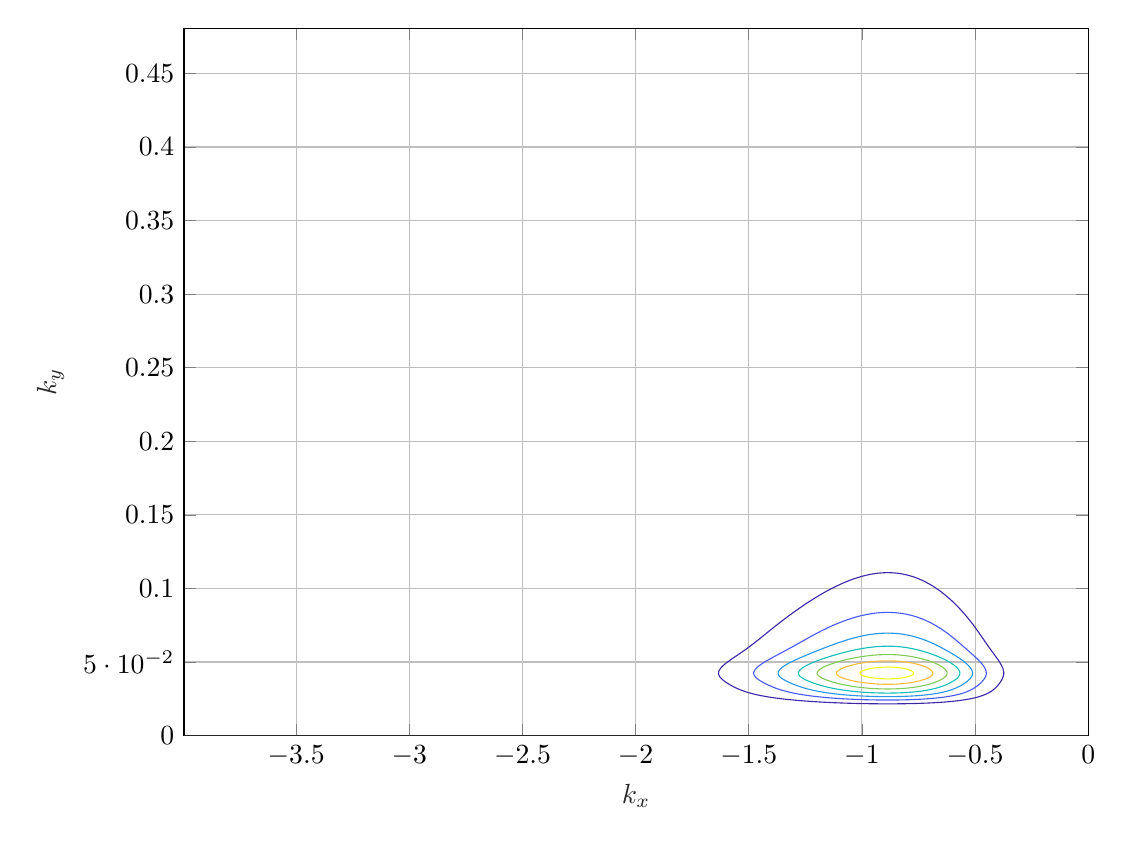
\begin{tikzpicture}

\begin{axis}[%
width=4.521in,
height=3.537in,
at={(0.758in,0.51in)},
scale only axis,
colormap={mymap}{[1pt] rgb(0pt)=(0.2422,0.1504,0.6603); rgb(1pt)=(0.2444,0.1534,0.6728); rgb(2pt)=(0.2464,0.1569,0.6847); rgb(3pt)=(0.2484,0.1607,0.6961); rgb(4pt)=(0.2503,0.1648,0.7071); rgb(5pt)=(0.2522,0.1689,0.7179); rgb(6pt)=(0.254,0.1732,0.7286); rgb(7pt)=(0.2558,0.1773,0.7393); rgb(8pt)=(0.2576,0.1814,0.7501); rgb(9pt)=(0.2594,0.1854,0.761); rgb(11pt)=(0.2628,0.1932,0.7828); rgb(12pt)=(0.2645,0.1972,0.7937); rgb(13pt)=(0.2661,0.2011,0.8043); rgb(14pt)=(0.2676,0.2052,0.8148); rgb(15pt)=(0.2691,0.2094,0.8249); rgb(16pt)=(0.2704,0.2138,0.8346); rgb(17pt)=(0.2717,0.2184,0.8439); rgb(18pt)=(0.2729,0.2231,0.8528); rgb(19pt)=(0.274,0.228,0.8612); rgb(20pt)=(0.2749,0.233,0.8692); rgb(21pt)=(0.2758,0.2382,0.8767); rgb(22pt)=(0.2766,0.2435,0.884); rgb(23pt)=(0.2774,0.2489,0.8908); rgb(24pt)=(0.2781,0.2543,0.8973); rgb(25pt)=(0.2788,0.2598,0.9035); rgb(26pt)=(0.2794,0.2653,0.9094); rgb(27pt)=(0.2798,0.2708,0.915); rgb(28pt)=(0.2802,0.2764,0.9204); rgb(29pt)=(0.2806,0.2819,0.9255); rgb(30pt)=(0.2809,0.2875,0.9305); rgb(31pt)=(0.2811,0.293,0.9352); rgb(32pt)=(0.2813,0.2985,0.9397); rgb(33pt)=(0.2814,0.304,0.9441); rgb(34pt)=(0.2814,0.3095,0.9483); rgb(35pt)=(0.2813,0.315,0.9524); rgb(36pt)=(0.2811,0.3204,0.9563); rgb(37pt)=(0.2809,0.3259,0.96); rgb(38pt)=(0.2807,0.3313,0.9636); rgb(39pt)=(0.2803,0.3367,0.967); rgb(40pt)=(0.2798,0.3421,0.9702); rgb(41pt)=(0.2791,0.3475,0.9733); rgb(42pt)=(0.2784,0.3529,0.9763); rgb(43pt)=(0.2776,0.3583,0.9791); rgb(44pt)=(0.2766,0.3638,0.9817); rgb(45pt)=(0.2754,0.3693,0.984); rgb(46pt)=(0.2741,0.3748,0.9862); rgb(47pt)=(0.2726,0.3804,0.9881); rgb(48pt)=(0.271,0.386,0.9898); rgb(49pt)=(0.2691,0.3916,0.9912); rgb(50pt)=(0.267,0.3973,0.9924); rgb(51pt)=(0.2647,0.403,0.9935); rgb(52pt)=(0.2621,0.4088,0.9946); rgb(53pt)=(0.2591,0.4145,0.9955); rgb(54pt)=(0.2556,0.4203,0.9965); rgb(55pt)=(0.2517,0.4261,0.9974); rgb(56pt)=(0.2473,0.4319,0.9983); rgb(57pt)=(0.2424,0.4378,0.9991); rgb(58pt)=(0.2369,0.4437,0.9996); rgb(59pt)=(0.2311,0.4497,0.9995); rgb(60pt)=(0.225,0.4559,0.9985); rgb(61pt)=(0.2189,0.462,0.9968); rgb(62pt)=(0.2128,0.4682,0.9948); rgb(63pt)=(0.2066,0.4743,0.9926); rgb(64pt)=(0.2006,0.4803,0.9906); rgb(65pt)=(0.195,0.4861,0.9887); rgb(66pt)=(0.1903,0.4919,0.9867); rgb(67pt)=(0.1869,0.4975,0.9844); rgb(68pt)=(0.1847,0.503,0.9819); rgb(69pt)=(0.1831,0.5084,0.9793); rgb(70pt)=(0.1818,0.5138,0.9766); rgb(71pt)=(0.1806,0.5191,0.9738); rgb(72pt)=(0.1795,0.5244,0.9709); rgb(73pt)=(0.1785,0.5296,0.9677); rgb(74pt)=(0.1778,0.5349,0.9641); rgb(75pt)=(0.1773,0.5401,0.9602); rgb(76pt)=(0.1768,0.5452,0.956); rgb(77pt)=(0.1764,0.5504,0.9516); rgb(78pt)=(0.1755,0.5554,0.9473); rgb(79pt)=(0.174,0.5605,0.9432); rgb(80pt)=(0.1716,0.5655,0.9393); rgb(81pt)=(0.1686,0.5705,0.9357); rgb(82pt)=(0.1649,0.5755,0.9323); rgb(83pt)=(0.161,0.5805,0.9289); rgb(84pt)=(0.1573,0.5854,0.9254); rgb(85pt)=(0.154,0.5902,0.9218); rgb(86pt)=(0.1513,0.595,0.9182); rgb(87pt)=(0.1492,0.5997,0.9147); rgb(88pt)=(0.1475,0.6043,0.9113); rgb(89pt)=(0.1461,0.6089,0.908); rgb(90pt)=(0.1446,0.6135,0.905); rgb(91pt)=(0.1429,0.618,0.9022); rgb(92pt)=(0.1408,0.6226,0.8998); rgb(93pt)=(0.1383,0.6272,0.8975); rgb(94pt)=(0.1354,0.6317,0.8953); rgb(95pt)=(0.1321,0.6363,0.8932); rgb(96pt)=(0.1288,0.6408,0.891); rgb(97pt)=(0.1253,0.6453,0.8887); rgb(98pt)=(0.1219,0.6497,0.8862); rgb(99pt)=(0.1185,0.6541,0.8834); rgb(100pt)=(0.1152,0.6584,0.8804); rgb(101pt)=(0.1119,0.6627,0.877); rgb(102pt)=(0.1085,0.6669,0.8734); rgb(103pt)=(0.1048,0.671,0.8695); rgb(104pt)=(0.1009,0.675,0.8653); rgb(105pt)=(0.0964,0.6789,0.8609); rgb(106pt)=(0.0914,0.6828,0.8562); rgb(107pt)=(0.0855,0.6865,0.8513); rgb(108pt)=(0.0789,0.6902,0.8462); rgb(109pt)=(0.0713,0.6938,0.8409); rgb(110pt)=(0.0628,0.6972,0.8355); rgb(111pt)=(0.0535,0.7006,0.8299); rgb(112pt)=(0.0433,0.7039,0.8242); rgb(113pt)=(0.0328,0.7071,0.8183); rgb(114pt)=(0.0234,0.7103,0.8124); rgb(115pt)=(0.0155,0.7133,0.8064); rgb(116pt)=(0.0091,0.7163,0.8003); rgb(117pt)=(0.0046,0.7192,0.7941); rgb(118pt)=(0.0019,0.722,0.7878); rgb(119pt)=(0.0009,0.7248,0.7815); rgb(120pt)=(0.0018,0.7275,0.7752); rgb(121pt)=(0.0046,0.7301,0.7688); rgb(122pt)=(0.0094,0.7327,0.7623); rgb(123pt)=(0.0162,0.7352,0.7558); rgb(124pt)=(0.0253,0.7376,0.7492); rgb(125pt)=(0.0369,0.74,0.7426); rgb(126pt)=(0.0504,0.7423,0.7359); rgb(127pt)=(0.0638,0.7446,0.7292); rgb(128pt)=(0.077,0.7468,0.7224); rgb(129pt)=(0.0899,0.7489,0.7156); rgb(130pt)=(0.1023,0.751,0.7088); rgb(131pt)=(0.1141,0.7531,0.7019); rgb(132pt)=(0.1252,0.7552,0.695); rgb(133pt)=(0.1354,0.7572,0.6881); rgb(134pt)=(0.1448,0.7593,0.6812); rgb(135pt)=(0.1532,0.7614,0.6741); rgb(136pt)=(0.1609,0.7635,0.6671); rgb(137pt)=(0.1678,0.7656,0.6599); rgb(138pt)=(0.1741,0.7678,0.6527); rgb(139pt)=(0.1799,0.7699,0.6454); rgb(140pt)=(0.1853,0.7721,0.6379); rgb(141pt)=(0.1905,0.7743,0.6303); rgb(142pt)=(0.1954,0.7765,0.6225); rgb(143pt)=(0.2003,0.7787,0.6146); rgb(144pt)=(0.2061,0.7808,0.6065); rgb(145pt)=(0.2118,0.7828,0.5983); rgb(146pt)=(0.2178,0.7849,0.5899); rgb(147pt)=(0.2244,0.7869,0.5813); rgb(148pt)=(0.2318,0.7887,0.5725); rgb(149pt)=(0.2401,0.7905,0.5636); rgb(150pt)=(0.2491,0.7922,0.5546); rgb(151pt)=(0.2589,0.7937,0.5454); rgb(152pt)=(0.2695,0.7951,0.536); rgb(153pt)=(0.2809,0.7964,0.5266); rgb(154pt)=(0.2929,0.7975,0.517); rgb(155pt)=(0.3052,0.7985,0.5074); rgb(156pt)=(0.3176,0.7994,0.4975); rgb(157pt)=(0.3301,0.8002,0.4876); rgb(158pt)=(0.3424,0.8009,0.4774); rgb(159pt)=(0.3548,0.8016,0.4669); rgb(160pt)=(0.3671,0.8021,0.4563); rgb(161pt)=(0.3795,0.8026,0.4454); rgb(162pt)=(0.3921,0.8029,0.4344); rgb(163pt)=(0.405,0.8031,0.4233); rgb(164pt)=(0.4184,0.803,0.4122); rgb(165pt)=(0.4322,0.8028,0.4013); rgb(166pt)=(0.4463,0.8024,0.3904); rgb(167pt)=(0.4608,0.8018,0.3797); rgb(168pt)=(0.4753,0.8011,0.3691); rgb(169pt)=(0.4899,0.8002,0.3586); rgb(170pt)=(0.5044,0.7993,0.348); rgb(171pt)=(0.5187,0.7982,0.3374); rgb(172pt)=(0.5329,0.797,0.3267); rgb(173pt)=(0.547,0.7957,0.3159); rgb(175pt)=(0.5748,0.7929,0.2941); rgb(176pt)=(0.5886,0.7913,0.2833); rgb(177pt)=(0.6024,0.7896,0.2726); rgb(178pt)=(0.6161,0.7878,0.2622); rgb(179pt)=(0.6297,0.7859,0.2521); rgb(180pt)=(0.6433,0.7839,0.2423); rgb(181pt)=(0.6567,0.7818,0.2329); rgb(182pt)=(0.6701,0.7796,0.2239); rgb(183pt)=(0.6833,0.7773,0.2155); rgb(184pt)=(0.6963,0.775,0.2075); rgb(185pt)=(0.7091,0.7727,0.1998); rgb(186pt)=(0.7218,0.7703,0.1924); rgb(187pt)=(0.7344,0.7679,0.1852); rgb(188pt)=(0.7468,0.7654,0.1782); rgb(189pt)=(0.759,0.7629,0.1717); rgb(190pt)=(0.771,0.7604,0.1658); rgb(191pt)=(0.7829,0.7579,0.1608); rgb(192pt)=(0.7945,0.7554,0.157); rgb(193pt)=(0.806,0.7529,0.1546); rgb(194pt)=(0.8172,0.7505,0.1535); rgb(195pt)=(0.8281,0.7481,0.1536); rgb(196pt)=(0.8389,0.7457,0.1546); rgb(197pt)=(0.8495,0.7435,0.1564); rgb(198pt)=(0.86,0.7413,0.1587); rgb(199pt)=(0.8703,0.7392,0.1615); rgb(200pt)=(0.8804,0.7372,0.165); rgb(201pt)=(0.8903,0.7353,0.1695); rgb(202pt)=(0.9,0.7336,0.1749); rgb(203pt)=(0.9093,0.7321,0.1815); rgb(204pt)=(0.9184,0.7308,0.189); rgb(205pt)=(0.9272,0.7298,0.1973); rgb(206pt)=(0.9357,0.729,0.2061); rgb(207pt)=(0.944,0.7285,0.2151); rgb(208pt)=(0.9523,0.7284,0.2237); rgb(209pt)=(0.9606,0.7285,0.2312); rgb(210pt)=(0.9689,0.7292,0.2373); rgb(211pt)=(0.977,0.7304,0.2418); rgb(212pt)=(0.9842,0.733,0.2446); rgb(213pt)=(0.99,0.7365,0.2429); rgb(214pt)=(0.9946,0.7407,0.2394); rgb(215pt)=(0.9966,0.7458,0.2351); rgb(216pt)=(0.9971,0.7513,0.2309); rgb(217pt)=(0.9972,0.7569,0.2267); rgb(218pt)=(0.9971,0.7626,0.2224); rgb(219pt)=(0.9969,0.7683,0.2181); rgb(220pt)=(0.9966,0.774,0.2138); rgb(221pt)=(0.9962,0.7798,0.2095); rgb(222pt)=(0.9957,0.7856,0.2053); rgb(223pt)=(0.9949,0.7915,0.2012); rgb(224pt)=(0.9938,0.7974,0.1974); rgb(225pt)=(0.9923,0.8034,0.1939); rgb(226pt)=(0.9906,0.8095,0.1906); rgb(227pt)=(0.9885,0.8156,0.1875); rgb(228pt)=(0.9861,0.8218,0.1846); rgb(229pt)=(0.9835,0.828,0.1817); rgb(230pt)=(0.9807,0.8342,0.1787); rgb(231pt)=(0.9778,0.8404,0.1757); rgb(232pt)=(0.9748,0.8467,0.1726); rgb(233pt)=(0.972,0.8529,0.1695); rgb(234pt)=(0.9694,0.8591,0.1665); rgb(235pt)=(0.9671,0.8654,0.1636); rgb(236pt)=(0.9651,0.8716,0.1608); rgb(237pt)=(0.9634,0.8778,0.1582); rgb(238pt)=(0.9619,0.884,0.1557); rgb(239pt)=(0.9608,0.8902,0.1532); rgb(240pt)=(0.9601,0.8963,0.1507); rgb(241pt)=(0.9596,0.9023,0.148); rgb(242pt)=(0.9595,0.9084,0.145); rgb(243pt)=(0.9597,0.9143,0.1418); rgb(244pt)=(0.9601,0.9203,0.1382); rgb(245pt)=(0.9608,0.9262,0.1344); rgb(246pt)=(0.9618,0.932,0.1304); rgb(247pt)=(0.9629,0.9379,0.1261); rgb(248pt)=(0.9642,0.9437,0.1216); rgb(249pt)=(0.9657,0.9494,0.1168); rgb(250pt)=(0.9674,0.9552,0.1116); rgb(251pt)=(0.9692,0.9609,0.1061); rgb(252pt)=(0.9711,0.9667,0.1001); rgb(253pt)=(0.973,0.9724,0.0938); rgb(254pt)=(0.9749,0.9782,0.0872); rgb(255pt)=(0.9769,0.9839,0.0805)},
xmin=-3.99549341800437,
xmax=0,
xlabel style={font=\color{white!15!black}},
xlabel={$k_{x}$},
ymin=0,
ymax=0.480677883608269,
ylabel style={font=\color{white!15!black}},
ylabel={$k_{y}$},
axis background/.style={fill=white},
xmajorgrids,
ymajorgrids
]
\addplot[contour prepared, contour prepared format=matlab, contour/labels=false] table[row sep=crcr] {%
%
0.005	615\\
-0.755938347711432	0.0218708335796425\\
-0.760918854415919	0.0218479569185073\\
-0.767758540070646	0.0218186272294896\\
-0.774628828345752	0.0217912719866442\\
-0.781529719241237	0.0217658417205903\\
-0.788461212757101	0.0217422906843998\\
-0.795423308893345	0.0217205767092487\\
-0.802416007649967	0.0217006610720749\\
-0.809439309026969	0.0216825083746312\\
-0.816493213024349	0.0216660864333786\\
-0.823577719642109	0.021651366179716\\
-0.830692828880248	0.0216383215700935\\
-0.837838540738765	0.0216269295056007\\
-0.845014855217662	0.0216171697606667\\
-0.852221772316938	0.0216090249205504\\
-0.859459292036593	0.0216024803273369\\
-0.866727414376628	0.0215975240341977\\
-0.874026139337041	0.021594146767705\\
-0.881355466917834	0.0215923418980287\\
-0.888715397119005	0.0215921054168763\\
-0.896105929940556	0.0215934359230722\\
-0.903527065382485	0.0215963346157018\\
-0.910978803444794	0.0216008052947815\\
-0.918461144127482	0.0216068543694459\\
-0.925974087430549	0.0216144908736745\\
-0.933517633353995	0.0216237264896141\\
-0.94109178189782	0.0216345755785838\\
-0.948696533062024	0.0216470552198822\\
-0.956331886846607	0.0216611852575496\\
-0.96399784325157	0.021676988355272\\
-0.971694402276911	0.0216944900596498\\
-0.979421563922632	0.0217137188720867\\
-0.987179328188732	0.0217347063295973\\
-0.99496769507521	0.0217574870948656\\
-1.00278666458207	0.0217820990559317\\
-1.01063623670931	0.0218085834359246\\
-1.01851641145692	0.0218369849133062\\
-1.02642718882492	0.0218673517531384\\
-1.02728862027772	0.0218708335796425\\
-1.03436856881329	0.0218981486038276\\
-1.04234055142204	0.0219307136011124\\
-1.05034313665118	0.0219652946102578\\
-1.05837632450069	0.0220019522727279\\
-1.06644011497058	0.0220407514166793\\
-1.07453450806085	0.0220817612566351\\
-1.0826595037715	0.022125055608514\\
-1.09081510210252	0.0221707131209914\\
-1.09900130305393	0.0222188175242522\\
-1.10721810662572	0.0222694578972834\\
-1.1079271275333	0.0222739741026576\\
-1.11546551281788	0.0223204123449869\\
-1.12374352163043	0.0223737537655685\\
-1.13205213306335	0.0224297986015511\\
-1.14039134711665	0.0224886550207235\\
-1.14876116379033	0.0225504378686066\\
-1.15716158308439	0.0226152690577291\\
-1.16529037980338	0.0226807962742846\\
-1.16559260499883	0.0226831776596654\\
-1.17405422953365	0.0227516183126857\\
-1.18254645668885	0.0228233798709646\\
-1.19106928646443	0.0228986107549261\\
-1.19962271886038	0.0229774684851165\\
-1.20820675387672	0.0230601202527463\\
-1.2113508493998	0.0230913000945237\\
-1.21682139151343	0.023144878514254\\
-1.22546663177053	0.0232326079368156\\
-1.234142474648	0.0233245506885638\\
-1.24284892014585	0.0234209120938217\\
-1.25019337133736	0.0235054855633748\\
-1.25158596826408	0.0235214644829499\\
-1.26035361900269	0.0236244578671368\\
-1.26915187236168	0.0237324271945599\\
-1.27798072834105	0.0238456271537823\\
-1.28383407049896	0.0239233526808379\\
-1.2868401869408	0.0239634711799871\\
-1.29573024816092	0.0240853572347932\\
-1.30465091200143	0.0242132117234233\\
-1.31344293415244	0.0243449014469129\\
-1.31360217846231	0.0243473172677454\\
-1.32258404754357	0.0244859780442554\\
-1.33159651924522	0.0246315240693008\\
-1.33982131536433	0.0247701318616\\
-1.34063959356724	0.0247842030198277\\
-1.34971327050964	0.0249431888941112\\
-1.35881755007242	0.0251102015932699\\
-1.36351333381447	0.0251990439248992\\
-1.36795243225558	0.0252853561445905\\
-1.37711791705911	0.0254690956422432\\
-1.38489438952795	0.0256316376368103\\
-1.38631400448303	0.0256623232022544\\
-1.39554069452733	0.0258657548095284\\
-1.40430012903311	0.0260679129973334\\
-1.404797987192	0.0260798659214223\\
-1.41408588247706	0.0263064825059535\\
-1.42199302765399	0.0265078700064685\\
-1.42340438038249	0.0265454730052639\\
-1.4327534809083	0.0267993974235814\\
-1.43816847889269	0.0269515086642157\\
-1.44213318405449	0.0270686213482722\\
-1.45154348982107	0.027354724954175\\
-1.4529679290991	0.0273988289705748\\
-1.46098439820801	0.0276610826523631\\
-1.46658810863077	0.027849830925546\\
-1.47045590921534	0.0279879920401411\\
-1.47909801427682	0.0283045145291292\\
-1.47995802284305	0.0283380253257745\\
-1.48949073909114	0.0287155881931983\\
-1.4906648653855	0.0287628797813244\\
-1.4990540579596	0.0291235268764456\\
-1.50137378821029	0.0292249266821316\\
-1.50864797944845	0.0295649721066249\\
-1.51130122571058	0.0296906552315508\\
-1.51827250355767	0.0300442720410201\\
-1.52053248581189	0.030160065429582\\
-1.52792763028728	0.0305660549540969\\
-1.52914130155664	0.0306331572762252\\
-1.53720438421852	0.0311099307714804\\
-1.53761335963726	0.0311356730973489\\
-1.54481920187105	0.0315903859153477\\
-1.54732969160762	0.0317596863816333\\
-1.5519973309855	0.0320745227078269\\
-1.55707662619836	0.0324400613372494\\
-1.55877905818227	0.0325623411489182\\
-1.56525140737708	0.0330538412386215\\
-1.56685416340948	0.0331821952790673\\
-1.57145771149733	0.0335490229769367\\
-1.57666230324098	0.0339890915644283\\
-1.57736234166022	0.034047886363864\\
-1.58309505986288	0.0345504313994033\\
-1.58650104569286	0.03486599338784\\
-1.58857789751986	0.0350566580835546\\
-1.5938695423279	0.035566566416318\\
-1.59637039076512	0.0358208213921423\\
-1.59895080407938	0.0360801563976933\\
-1.60381342777846	0.0365974280276806\\
-1.60627033845775	0.0368760153905426\\
-1.60843831477895	0.03711838130628\\
-1.61281384893536	0.0376430162334913\\
-1.61620088877077	0.0380871508733661\\
-1.61685412518648	0.0381713328093147\\
-1.6206242090547	0.0387033310337501\\
-1.62396930744422	0.0392390109067974\\
-1.62616204170416	0.0396467788356241\\
-1.62688640512822	0.0397783724284569\\
-1.62938402221197	0.0403214155987283\\
-1.63134788539712	0.0408681404176117\\
-1.63274947658685	0.0414185468851071\\
-1.63356314466305	0.0419726350012145\\
-1.63376691489158	0.042530404765934\\
-1.63334318277323	0.0430918561792654\\
-1.63227998436755	0.0436569892412089\\
-1.63067884902791	0.0442258039517643\\
-1.62861740695224	0.0447983003109318\\
-1.62616204170416	0.0453597397468779\\
-1.62609920919489	0.0453744783187113\\
-1.62323189875118	0.0459543379751028\\
-1.61992956634594	0.0465378792801063\\
-1.61620088877077	0.0471247602877373\\
-1.61619875743385	0.0471251022337218\\
-1.61219770763277	0.0477160068359494\\
-1.60780213930552	0.0483105930867889\\
-1.60627033845775	0.0485052957187258\\
-1.60313931976355	0.0489088609862404\\
-1.59817615817887	0.049510810534304\\
-1.59637039076512	0.0497203968695551\\
-1.59299555269274	0.0501164417309796\\
-1.5875677852954	0.0507257545762672\\
-1.58650104569286	0.0508425108414429\\
-1.58200670292482	0.0513387490701667\\
-1.57666230324098	0.0519093930032816\\
-1.57623439568554	0.0519554252126783\\
-1.57040541422009	0.0525757830038019\\
-1.56685416340948	0.0529465522716895\\
-1.56444304583573	0.0531998224435376\\
-1.55840784473733	0.0538275435318852\\
-1.55707662619836	0.0539659182892671\\
-1.55235805783457	0.0544589462688448\\
-1.54732969160762	0.0549804212342966\\
-1.54623913787107	0.0550940306544164\\
-1.54015041100038	0.0557327966886001\\
-1.53761335963726	0.0559998376917894\\
-1.53406154480569	0.0563752443713957\\
-1.52795451022657	0.0570213737028034\\
-1.52792763028728	0.0570242689094148\\
-1.52194548166784	0.0576711846828231\\
-1.51827250355767	0.0580698868324593\\
-1.51593372339703	0.0583246773114548\\
-1.50996350420012	0.0589818515886985\\
-1.50864797944845	0.0591288524207096\\
-1.5040659188261	0.0596427075145542\\
-1.4990540579596	0.0602077683322201\\
-1.49817456159958	0.0603072450890219\\
-1.49236701595952	0.0609754643121017\\
-1.48949073909114	0.0613091624393078\\
-1.48658482630316	0.0616473651837934\\
-1.48082422937032	0.0623229477040971\\
-1.47995802284305	0.0624260685934561\\
-1.47513310366752	0.0630022118730129\\
-1.47045590921534	0.0635619739471087\\
-1.46942923368344	0.0636851576905407\\
-1.46377729717028	0.0643717851566804\\
-1.46098439820801	0.0647125051911031\\
-1.45812520786654	0.0650620942714322\\
-1.45246489831529	0.065756085034796\\
-1.45154348982107	0.0658700988251399\\
-1.44683520901436	0.0664537574467718\\
-1.44213318405449	0.0670349258974961\\
-1.44116195244527	0.0671551115073596\\
-1.43550308734357	0.0678601472165594\\
-1.4327534809083	0.0682023821374733\\
-1.42981083393808	0.0685688645743713\\
-1.42407502421041	0.0692812635807951\\
-1.42340438038249	0.0693649847575489\\
-1.41833857130262	0.069997344235831\\
-1.41408588247706	0.0705248190412798\\
-1.41253431407418	0.0707171065394788\\
-1.40669911122905	0.0714405504917387\\
-1.404797987192	0.0716759398703197\\
-1.4008201471781	0.0721676760926106\\
-1.39554069452733	0.0728157524030019\\
-1.39486512101548	0.0728984833420945\\
-1.38888077355354	0.0736329722401904\\
-1.38631400448303	0.073946529799332\\
-1.38282688177112	0.0743711427868983\\
-1.37711791705911	0.0750615875530988\\
-1.37669111809474	0.0751129949822182\\
-1.37051639833701	0.0758585288261501\\
-1.36795243225558	0.0761665562140715\\
-1.3642618420513	0.0766077443186941\\
-1.35881755007242	0.0772546849063036\\
-1.3579206821124	0.07736064145985\\
-1.35152027119691	0.078117220249618\\
-1.34971327050964	0.0783303149865896\\
-1.3450421805219	0.0788774806879979\\
-1.34063959356724	0.0793907065467796\\
-1.33847249878895	0.0796414227749899\\
-1.33181412670334	0.0804090465105939\\
-1.33159651924522	0.0804342097133059\\
-1.32508890642974	0.0811803518948099\\
-1.32258404754357	0.0814665502648136\\
-1.31826568842489	0.0819553389276379\\
-1.31360217846231	0.0824817005956845\\
-1.31134361220257	0.0827340076090779\\
-1.30465091200143	0.0834800322358954\\
-1.30432135178006	0.0835163579391299\\
-1.29721128139619	0.084302389917794\\
-1.29573024816092	0.0844660560844381\\
-1.28999577228534	0.08509210354507\\
-1.2868401869408	0.0854363452417795\\
-1.28266862837003	0.085885498820958\\
-1.27798072834105	0.0863901938531484\\
-1.27522650754913	0.0866825757454581\\
-1.26915187236168	0.0873277963459003\\
-1.26766537102176	0.0874833343185702\\
-1.26035361900269	0.0882492989704053\\
-1.25998042116331	0.0882877745402943\\
-1.2521688525393	0.0890958964106304\\
-1.25158596826408	0.0891563757347774\\
-1.24422092324414	0.0899076999295784\\
-1.24284892014585	0.0900480160708609\\
-1.23612734695441	0.0907231850971386\\
-1.234142474648	0.0909231918811428\\
-1.22787996360161	0.0915423519133107\\
-1.22546663177053	0.0917818540063116\\
-1.21946943978761	0.0923652003780948\\
-1.21682139151343	0.092623906621502\\
-1.21088513922219	0.0931917304914909\\
-1.20820675387672	0.093449207691584\\
-1.20211497263092	0.0940219422534991\\
-1.19962271886038	0.0942575693100975\\
-1.19314522340055	0.0948558356641192\\
-1.19106928646443	0.0950487579043785\\
-1.18396034445934	0.0956934107233514\\
-1.18254645668885	0.095822494295149\\
-1.17454272092732	0.0965346674311956\\
-1.17405422953365	0.0965784536028746\\
-1.16559260499883	0.0973179482011682\\
-1.16486771478451	0.0973796057876518\\
-1.15716158308439	0.0980406379595306\\
-1.15490922584174	0.09822822579272\\
-1.14876116379033	0.0987449094306291\\
-1.14464241256238	0.0990805274464002\\
-1.14039134711665	0.0994302645225806\\
-1.13403606166461	0.0999365107486924\\
-1.13205213306335	0.100096157491128\\
-1.12374352163043	0.100743438766621\\
-1.12304505727275	0.100796175699597\\
-1.11546551281788	0.101374930973523\\
-1.11159839067759	0.101659522299113\\
-1.10721810662572	0.10198570150127\\
-1.09966950110391	0.102526550547241\\
-1.09900130305393	0.102575020433874\\
-1.09081510210252	0.103148917611086\\
-1.08712439387746	0.103397260443981\\
-1.0826595037715	0.103701753325531\\
-1.07453450806085	0.104232435648417\\
-1.07391031877814	0.104271651989334\\
-1.06644011497058	0.104747833136484\\
-1.05982203282569	0.105149725183298\\
-1.05837632450069	0.105238845934741\\
-1.05034313665118	0.105713178369005\\
-1.04466861421925	0.106031480025874\\
-1.04234055142204	0.106164184569842\\
-1.03436856881329	0.10659712409609\\
-1.02814041972617	0.106916916517062\\
-1.02642718882492	0.107006404609464\\
-1.01851641145692	0.107398418143536\\
-1.01063623670931	0.107765060296052\\
-1.00970239886518	0.107806034656863\\
-1.00278666458207	0.108115210361388\\
-0.99496769507521	0.108441649890776\\
-0.98834563468107	0.108698834445275\\
-0.987179328188732	0.108745034857709\\
-0.979421563922632	0.109031036345694\\
-0.971694402276911	0.10929307232439\\
-0.96399784325157	0.109531572556817\\
-0.96173704615804	0.109595315882299\\
-0.956331886846607	0.109751082502401\\
-0.948696533062024	0.109948915896088\\
-0.94109178189782	0.110123642237814\\
-0.933517633353995	0.110275539362211\\
-0.925974087430549	0.11040484639501\\
-0.919607977548308	0.110495478967936\\
-0.918461144127482	0.110512210751347\\
-0.910978803444794	0.110599224517959\\
-0.903527065382485	0.110663533630943\\
-0.896105929940556	0.110705230283397\\
-0.888715397119005	0.110724369137194\\
-0.881355466917834	0.110720967440745\\
-0.874026139337041	0.110695005038643\\
-0.866727414376628	0.110646424273041\\
-0.859459292036593	0.110575129776213\\
-0.853333744216628	0.110495478967936\\
-0.852221772316938	0.110481374715864\\
-0.845014855217662	0.110367339537814\\
-0.837838540738765	0.110230694221838\\
-0.830692828880248	0.110071194945701\\
-0.823577719642109	0.109888558532997\\
-0.816493213024349	0.109682461577946\\
-0.813810674841223	0.109595315882299\\
-0.809439309026969	0.109456349831547\\
-0.802416007649967	0.109208978348974\\
-0.795423308893345	0.108937582832723\\
-0.789798374283232	0.108698834445275\\
-0.788461212757101	0.10864320673005\\
-0.781529719241237	0.108330838725324\\
-0.774628828345752	0.107993545648167\\
-0.771063445868687	0.107806034656863\\
-0.767758540070646	0.107635402319369\\
-0.760918854415919	0.107256777638349\\
-0.755193275214789	0.106916916517062\\
-0.754109771381571	0.106853710101818\\
-0.747331290967602	0.106433520437933\\
-0.741257773249516	0.106031480025874\\
-0.740583413174013	0.105987562295621\\
-0.733866138000802	0.105525281818341\\
-0.728729186845149	0.105149725183298\\
-0.727179465447971	0.105038137714001\\
-0.720523395515518	0.104532945058435\\
-0.717261439908291	0.104271651989334\\
-0.713897928203445	0.104006001181487\\
-0.707303063511751	0.103456772755007\\
-0.706620457940267	0.103397260443981\\
-0.700738801440436	0.102891103547292\\
-0.696711052271481	0.102526550547241\\
-0.6942051419895	0.102302546493851\\
-0.687702085158943	0.101692774184811\\
-0.68736178554515	0.101659522299113\\
-0.681229630948765	0.101067079167689\\
-0.678549518173803	0.100796175699597\\
-0.674787779358966	0.100420011694074\\
-0.670158975449137	0.0999365107486924\\
-0.668376530389547	0.0997522120254341\\
-0.662148106592559	0.0990805274464002\\
-0.661995884040506	0.0990642683413111\\
-0.655645840311844	0.0983602294799441\\
-0.654500546192145	0.09822822579272\\
-0.649326399203562	0.0976368846284039\\
-0.647158891747097	0.0973796057876518\\
-0.643037560715659	0.0968942394455495\\
-0.640093975100417	0.0965346674311956\\
-0.636779324848135	0.0961326947677084\\
-0.633282621629158	0.0956934107233514\\
-0.63055169160099	0.0953526022632597\\
-0.626704377262525	0.0948558356641192\\
-0.624354660974223	0.0945542646891851\\
-0.620341156083061	0.0940219422534991\\
-0.618188232967837	0.0937379359683293\\
-0.614176941329163	0.0931917304914909\\
-0.612052407581829	0.09290382108896\\
-0.608197530688152	0.0923652003780948\\
-0.6059471848162	0.0920520758298827\\
-0.602390318494937	0.0915423519133107\\
-0.59987256467095	0.0911828063170614\\
-0.596744108815605	0.0907231850971386\\
-0.59382854714608	0.0902960684217547\\
-0.591248954479506	0.0899076999295784\\
-0.587815132241588	0.0893918670160067\\
-0.585896017989385	0.0890958964106304\\
-0.581832319957476	0.0884701551094348\\
-0.580677450933755	0.0882877745402943\\
-0.575880110293743	0.087530832902213\\
-0.575586289084977	0.0874833343185702\\
-0.570617312509286	0.0866825757454581\\
-0.569958503250389	0.0865765557394078\\
-0.565763012853964	0.085885498820958\\
-0.564067498827413	0.0856060656971499\\
-0.561017661720752	0.08509210354507\\
-0.558207097024817	0.0846178682596958\\
-0.556376846020225	0.084302389917794\\
-0.552377297842601	0.0836116444127438\\
-0.551836693206074	0.0835163579391299\\
-0.547391905148615	0.0827340076090779\\
-0.546578101280763	0.0825907465354429\\
-0.543037991069677	0.0819553389276379\\
-0.540809507339304	0.0815539704775669\\
-0.53877305753733	0.0811803518948099\\
-0.535071516018224	0.0804984239135297\\
-0.534594807421209	0.0804090465105939\\
-0.530495526625574	0.0796414227749899\\
-0.529364127317524	0.0794290461698929\\
-0.526474135809923	0.0788774806879979\\
-0.523687341237202	0.0783426354941249\\
-0.522531107490831	0.078117220249618\\
-0.518660910800871	0.07736064145985\\
-0.51804115777726	0.0772395026670398\\
-0.514856409914316	0.0766077443186941\\
-0.512425576937697	0.0761222344998128\\
-0.511123451043303	0.0758585288261501\\
-0.507455865538003	0.0751129949822182\\
-0.506840598718512	0.0749879581679379\\
-0.503844538748665	0.0743711427868983\\
-0.501286223119707	0.0738403601852374\\
-0.500298651264284	0.0736329722401904\\
-0.496806679283428	0.0728984833420945\\
-0.495762450141281	0.0726784439845321\\
-0.493365588960508	0.0721676760926106\\
-0.490269279783234	0.0715025261103268\\
-0.489983761720597	0.0714405504917387\\
-0.486638306909718	0.0707171065394788\\
-0.484806712045567	0.0703187335396727\\
-0.483343166031317	0.069997344235831\\
-0.480091126931507	0.0692812635807951\\
-0.479374746928278	0.0691239679520586\\
-0.476868886084988	0.0685688645743713\\
-0.473973384431368	0.067923318744129\\
-0.473692323002892	0.0678601472165594\\
-0.470531854493427	0.0671551115073596\\
-0.468602624554837	0.0667234726231281\\
-0.467406110303056	0.0664537574467718\\
-0.464301084027397	0.065756085034796\\
-0.463262467298686	0.0655239849900916\\
-0.461209937024485	0.0650620942714322\\
-0.458144666970102	0.0643717851566804\\
-0.457952912662914	0.0643292008397682\\
-0.455071853838044	0.0636851576905407\\
-0.452673960647521	0.0631491439448016\\
-0.452020597818828	0.0630022118730129\\
-0.448961834385142	0.0623229477040971\\
-0.447425611252506	0.0619841626101747\\
-0.445907239963858	0.0616473651837934\\
-0.442854646998706	0.0609754643121017\\
-0.442207864477871	0.0608352581161402\\
-0.43978590065716	0.0603072450890219\\
-0.437020720323615	0.0597066829481266\\
-0.436727698633189	0.0596427075145542\\
-0.433644894370869	0.0589818515886985\\
-0.431864178789738	0.0586024975584883\\
-0.430566836686426	0.0583246773114548\\
-0.427486227099716	0.0576711846828231\\
-0.42673823987624	0.0575146017163532\\
-0.424394172110537	0.0570213737028034\\
-0.421642903583122	0.0564430784799719\\
-0.421321678311846	0.0563752443713957\\
-0.418237693494482	0.0557327966886001\\
-0.416578169910382	0.0553870516102278\\
-0.415177850463938	0.0550940306544164\\
-0.412144288649819	0.0544589462688448\\
-0.411544038858022	0.0543337078487372\\
-0.40912730899425	0.0538275435318852\\
-0.40654051042604	0.0532786564492382\\
-0.406170095256216	0.0531998224435376\\
-0.403244082291703	0.0525757830038019\\
-0.401567584614438	0.0522112731763696\\
-0.400393009392483	0.0519554252126783\\
-0.397615958401038	0.0513387490701667\\
-0.396625261423215	0.0511133752734446\\
-0.394921563723999	0.0507257545762672\\
-0.392339912313594	0.0501164417309796\\
-0.39171354085237	0.0499633964973879\\
-0.389857150462452	0.049510810534304\\
-0.387517232806171	0.0489088609862404\\
-0.386832422901905	0.0487231377160627\\
-0.385303381340041	0.0483105930867889\\
-0.383249178938984	0.0477160068359494\\
-0.381981907571819	0.047318017153108\\
-0.381362218084077	0.0471251022337218\\
-0.379633806474977	0.0465378792801063\\
-0.378103932476678	0.0459543379751028\\
-0.377161994862112	0.0455448326504166\\
-0.376764287383266	0.0453744783187113\\
-0.375606665963726	0.0447983003109318\\
-0.374659919379542	0.0442258039517643\\
-0.373924575208816	0.0436569892412089\\
-0.373436286223755	0.0430918561792654\\
-0.373241681223504	0.042530404765934\\
-0.373335265598294	0.0419726350012145\\
-0.373708954231558	0.0414185468851071\\
-0.37435265491418	0.0408681404176117\\
-0.375254587005457	0.0403214155987283\\
-0.376401653163925	0.0397783724284569\\
-0.377161994862112	0.0394789292204609\\
-0.377762312601035	0.0392390109067974\\
-0.379311998828793	0.0387033310337501\\
-0.381058568396491	0.0381713328093147\\
-0.381981907571819	0.0379160877283267\\
-0.382961234616668	0.0376430162334913\\
-0.385006074350883	0.03711838130628\\
-0.386832422901905	0.0366849873958929\\
-0.387199419811489	0.0365974280276806\\
-0.38949193817004	0.0360801563976933\\
-0.39171354085237	0.0356111606811582\\
-0.39192420979558	0.035566566416318\\
-0.394441116155405	0.0350566580835546\\
-0.396625261423215	0.0346398473084971\\
-0.397093680304832	0.0345504313994033\\
-0.399844683256408	0.034047886363864\\
-0.401567584614438	0.0337502093776363\\
-0.402734584250726	0.0335490229769367\\
-0.405765572333602	0.0330538412386215\\
-0.40654051042604	0.0329336244265221\\
-0.408945957741041	0.0325623411489182\\
-0.411544038858022	0.032186336167104\\
-0.412322111262039	0.0320745227078269\\
-0.415900213271366	0.0315903859153477\\
-0.416578169910382	0.031504113309545\\
-0.419709509014287	0.0311099307714804\\
-0.421642903583122	0.0308829001892226\\
-0.423798425492091	0.0306331572762252\\
-0.42673823987624	0.0303156287974584\\
-0.428202031902794	0.030160065429582\\
-0.431864178789738	0.0297972496793779\\
-0.432960976910717	0.0296906552315508\\
-0.437020720323615	0.02932258963936\\
-0.438122392082891	0.0292249266821316\\
-0.442207864477871	0.0288866013247884\\
-0.443741102341567	0.0287628797813244\\
-0.447425611252506	0.0284845779102733\\
-0.44988120009478	0.0283045145291292\\
-0.452673960647521	0.0281123103319128\\
-0.456618057534587	0.027849830925546\\
-0.457952912662914	0.0277661839195541\\
-0.463262467298686	0.0274440248156604\\
-0.464029127457633	0.0273988289705748\\
-0.468602624554837	0.0271438323697324\\
-0.472203705425871	0.0269515086642157\\
-0.473973384431368	0.026861740188442\\
-0.479374746928278	0.0265971958970046\\
-0.481266266812638	0.0265078700064685\\
-0.484806712045567	0.0263482241677479\\
-0.490269279783234	0.0261131192819959\\
-0.491352807206171	0.0260679129973334\\
-0.495762450141281	0.0258912432653967\\
-0.501286223119707	0.0256810320838739\\
-0.502627375275194	0.0256316376368103\\
-0.506840598718512	0.0254817276563904\\
-0.512425576937697	0.0252925835208492\\
-0.515304983908811	0.0251990439248992\\
-0.51804115777726	0.0251126250723588\\
-0.523687341237202	0.0249413190681204\\
-0.529364127317524	0.024778529677478\\
-0.529665116757637	0.0247701318616\\
-0.535071516018224	0.0246224071241428\\
-0.540809507339304	0.0244738787580051\\
-0.546062576870555	0.0243449014469129\\
-0.546578101280763	0.0243324190177055\\
-0.552377297842601	0.0241959665317556\\
-0.558207097024817	0.0240661118529822\\
-0.564067498827413	0.0239425069861289\\
-0.565005163484916	0.0239233526808379\\
-0.569958503250389	0.0238227201761071\\
-0.575880110293743	0.0237082620533524\\
-0.581832319957476	0.0235992491268377\\
-0.587221284345304	0.0235054855633748\\
-0.587815132241588	0.0234951254876482\\
-0.59382854714608	0.0233934357580327\\
-0.59987256467095	0.0232965469203439\\
-0.6059471848162	0.0232042253428065\\
-0.612052407581829	0.0231162515707885\\
-0.613850639874028	0.0230913000945237\\
-0.618188232967837	0.023030369827951\\
-0.624354660974223	0.0229477048061566\\
-0.63055169160099	0.0228689365593588\\
-0.636779324848135	0.022793887882555\\
-0.643037560715659	0.0227223921501997\\
-0.646850267296592	0.0226807962742846\\
-0.649326399203562	0.0226531760924003\\
-0.655645840311844	0.0225855933853236\\
-0.661995884040506	0.022521251976534\\
-0.668376530389547	0.0224600160049549\\
-0.674787779358966	0.0224017576920213\\
-0.681229630948765	0.0223463568716768\\
-0.687702085158943	0.0222937005533663\\
-0.690243299705289	0.0222739741026576\\
-0.6942051419895	0.0222421713949123\\
-0.700738801440436	0.0221923232493968\\
-0.707303063511751	0.0221450417180306\\
-0.713897928203445	0.0221002343300088\\
-0.720523395515518	0.0220578142939029\\
-0.727179465447971	0.0220177002013276\\
-0.733866138000802	0.0219798157516261\\
-0.740583413174013	0.0219440894962016\\
-0.747331290967602	0.021910454601226\\
-0.754109771381571	0.0218788486275647\\
-0.755938347711432	0.0218708335796425\\
0.01	477\\
-0.804377221313069	0.0243449014469129\\
-0.809439309026969	0.0243241307640515\\
-0.816493213024349	0.0242980172511584\\
-0.823577719642109	0.0242746096936781\\
-0.830692828880248	0.0242538666782013\\
-0.837838540738765	0.0242357514737661\\
-0.845014855217662	0.0242202319184805\\
-0.852221772316938	0.0242072803201208\\
-0.859459292036593	0.0241968733702583\\
-0.866727414376628	0.024188992071525\\
-0.874026139337041	0.0241836216776877\\
-0.881355466917834	0.0241807516462561\\
-0.888715397119005	0.0241803756034042\\
-0.896105929940556	0.0241824913210387\\
-0.903527065382485	0.0241871007058971\\
-0.910978803444794	0.0241942098006134\\
-0.918461144127482	0.0242038287967364\\
-0.925974087430549	0.0242159720597382\\
-0.933517633353995	0.0242306581661007\\
-0.94109178189782	0.0242479099526179\\
-0.948696533062024	0.0242677545781062\\
-0.956331886846607	0.0242902235977629\\
-0.96399784325157	0.0243153530504737\\
-0.971694402276911	0.0243431835594184\\
-0.972131100348352	0.0243449014469129\\
-0.979421563922632	0.0243733280118298\\
-0.987179328188732	0.0244062013454073\\
-0.99496769507521	0.0244418835949337\\
-1.00278666458207	0.0244804341056716\\
-1.01063623670931	0.0245219174467415\\
-1.01851641145692	0.0245664035994634\\
-1.02642718882492	0.024613968162965\\
-1.03436856881329	0.0246646925779392\\
-1.04234055142204	0.0247186643695181\\
-1.04953495253661	0.0247701318616\\
-1.05034313665118	0.0247759229226535\\
-1.05837632450069	0.0248361114081239\\
-1.06644011497058	0.02489981600778\\
-1.07453450806085	0.0249671503654559\\
-1.0826595037715	0.0250382356800511\\
-1.09081510210252	0.0251132010854041\\
-1.09900130305393	0.0251921840587207\\
-1.09968842658144	0.0251990439248992\\
-1.10721810662572	0.0252750302960606\\
-1.11546551281788	0.0253621518288204\\
-1.12374352163043	0.0254537403057765\\
-1.13205213306335	0.0255499706107239\\
-1.13881292215278	0.0256316376368103\\
-1.14039134711665	0.0256510507273152\\
-1.14876116379033	0.0257572550967641\\
-1.15716158308439	0.0258686995477288\\
-1.16559260499883	0.0259856065132561\\
-1.171308382622	0.0260679129973334\\
-1.17405422953365	0.0261084507477863\\
-1.18254645668885	0.0262377668227145\\
-1.19106928646443	0.0263733347069774\\
-1.19917599767789	0.0265078700064685\\
-1.19962271886038	0.0265155166481849\\
-1.20820675387672	0.0266659998675478\\
-1.21682139151343	0.0268237139776552\\
-1.22353916340034	0.0269515086642157\\
-1.22546663177053	0.0269895425814385\\
-1.234142474648	0.0271652662903012\\
-1.24284892014585	0.0273494350605541\\
-1.24512467028638	0.0273988289705748\\
-1.25158596826408	0.0275450593419182\\
-1.26035361900269	0.0277510483265346\\
-1.26443314898441	0.027849830925546\\
-1.26915187236168	0.0279694758481234\\
-1.27798072834105	0.0282006833157385\\
-1.28183181814757	0.0283045145291292\\
-1.2868401869408	0.0284464347647729\\
-1.29573024816092	0.0287067707673443\\
-1.29760318111818	0.0287628797813244\\
-1.30465091200143	0.0289854762682231\\
-1.31198020516963	0.0292249266821316\\
-1.31360217846231	0.0292809016329018\\
-1.32258404754357	0.0295977864223809\\
-1.32515326590878	0.0296906552315508\\
-1.33159651924522	0.029937124870737\\
-1.3372748196482	0.030160065429582\\
-1.34063959356724	0.0302999476876293\\
-1.34847269576132	0.0306331572762252\\
-1.34971327050964	0.0306890290140477\\
-1.35881755007242	0.0311073156414761\\
-1.35887361647227	0.0311099307714804\\
-1.36795243225558	0.0315581892616901\\
-1.36859375013575	0.0315903859153477\\
-1.37711791705911	0.0320428027434456\\
-1.37770710432257	0.0320745227078269\\
-1.38629305500815	0.0325623411489182\\
-1.38631400448303	0.0325635917600528\\
-1.39443798239201	0.0330538412386215\\
-1.39554069452733	0.0331237790075846\\
-1.40218594691251	0.0335490229769367\\
-1.404797987192	0.0337244544249736\\
-1.4095792864592	0.034047886363864\\
-1.41408588247706	0.0343676234018784\\
-1.41664840778149	0.0345504313994033\\
-1.42340438038249	0.0350561157494074\\
-1.42341159799414	0.0350566580835546\\
-1.42993816256341	0.035566566416318\\
-1.4327534809083	0.0357983941677894\\
-1.4361702294528	0.0360801563976933\\
-1.44209024096357	0.0365974280276806\\
-1.44213318405449	0.0366013815811639\\
-1.44775561024502	0.03711838130628\\
-1.45154348982107	0.0374941010793685\\
-1.45304951466801	0.0376430162334913\\
-1.45799315701663	0.0381713328093147\\
-1.46098439820801	0.0385250154816472\\
-1.46250269057418	0.0387033310337501\\
-1.46657003296878	0.0392390109067974\\
-1.47008453000994	0.0397783724284569\\
-1.47045590921534	0.0398466049368106\\
-1.47307525118449	0.0403214155987283\\
-1.47543434956648	0.0408681404176117\\
-1.47711801650055	0.0414185468851071\\
-1.47809543848012	0.0419726350012145\\
-1.47834021826929	0.042530404765934\\
-1.47783120839409	0.0430918561792654\\
-1.47655403712395	0.0436569892412089\\
-1.47463066699427	0.0442258039517643\\
-1.47215435158593	0.0447983003109318\\
-1.47045590921534	0.0451231997331659\\
-1.46915980423348	0.0453744783187113\\
-1.46567340952453	0.0459543379751028\\
-1.46165806676661	0.0465378792801063\\
-1.46098439820801	0.0466264004715795\\
-1.45721557147711	0.0471251022337218\\
-1.45229118407497	0.0477160068359494\\
-1.45154348982107	0.0477996627393414\\
-1.44699106789972	0.0483105930867889\\
-1.44213318405449	0.0488184790177547\\
-1.44126954673455	0.0489088609862404\\
-1.43522713516224	0.049510810534304\\
-1.4327534809083	0.0497463903289186\\
-1.42886020854464	0.0501164417309796\\
-1.42340438038249	0.0506153033606723\\
-1.42219207624339	0.0507257545762672\\
-1.41528845388748	0.0513387490701667\\
-1.41408588247706	0.0514435722909148\\
-1.40818073473732	0.0519554252126783\\
-1.404797987192	0.052243909954019\\
-1.4008799728383	0.0525757830038019\\
-1.39554069452733	0.0530234573312205\\
-1.39342067663213	0.0531998224435376\\
-1.38631400448303	0.0537881799783341\\
-1.3858343436145	0.0538275435318852\\
-1.3781674671552	0.0544589462688448\\
-1.37711791705911	0.0545458226127651\\
-1.37043153747169	0.0550940306544164\\
-1.36795243225558	0.0552986906260129\\
-1.36264002656672	0.0557327966886001\\
-1.35881755007242	0.0560482331353964\\
-1.35481172330048	0.0563752443713957\\
-1.34971327050964	0.0567965753715615\\
-1.34696190716407	0.0570213737028034\\
-1.34063959356724	0.0575453052287244\\
-1.33910241001668	0.0576711846828231\\
-1.33159651924522	0.0582955294323516\\
-1.33124172591043	0.0583246773114548\\
-1.32339510768376	0.0589818515886985\\
-1.32258404754357	0.0590510097243626\\
-1.31555730022327	0.0596427075145542\\
-1.31360217846231	0.0598101811092427\\
-1.30772315174896	0.0603072450890219\\
-1.30465091200143	0.0605714819000934\\
-1.29988966923131	0.0609754643121017\\
-1.29573024816092	0.0613343840060109\\
-1.29205156196097	0.0616473651837934\\
-1.2868401869408	0.0620980753273685\\
-1.28420150014653	0.0623229477040971\\
-1.27798072834105	0.0628615097859137\\
-1.27633036104792	0.0630022118730129\\
-1.26915187236168	0.0636234615969501\\
-1.26842745394948	0.0636851576905407\\
-1.26048146154921	0.0643717851566804\\
-1.26035361900269	0.0643829970995432\\
-1.2524812104185	0.0650620942714322\\
-1.25158596826408	0.0651402408670187\\
-1.24440755056038	0.065756085034796\\
-1.24284892014585	0.0658912807559066\\
-1.23624534369705	0.0664537574467718\\
-1.234142474648	0.0666347134942917\\
-1.22797855229069	0.0671551115073596\\
-1.22546663177053	0.0673692095077424\\
-1.21959023842266	0.0678601472165594\\
-1.21682139151343	0.0680935345412937\\
-1.21106251599034	0.0685688645743713\\
-1.20820675387672	0.0688065614543625\\
-1.202376455522	0.0692812635807951\\
-1.19962271886038	0.0695072732207551\\
-1.19351194065745	0.069997344235831\\
-1.19106928646443	0.0701947586462383\\
-1.18444747473268	0.0707171065394788\\
-1.18254645668885	0.0708682025491186\\
-1.17515993492823	0.0714405504917387\\
-1.17405422953365	0.0715268721630858\\
-1.16562427007291	0.0721676760926106\\
-1.16559260499883	0.072170101368872\\
-1.15716158308439	0.0727998888549238\\
-1.1558025791979	0.0728984833420945\\
-1.14876116379033	0.07341355628924\\
-1.14566822246491	0.0736329722401904\\
-1.14039134711665	0.0740104991128655\\
-1.13518605505927	0.0743711427868983\\
-1.13205213306335	0.0745901841700147\\
-1.12431647339254	0.0751129949822182\\
-1.12374352163043	0.0751520726575404\\
-1.11546551281788	0.0756996845877829\\
-1.11297713738834	0.0758585288261501\\
-1.10721810662572	0.0762298792363737\\
-1.10112796883184	0.0766077443186941\\
-1.09900130305393	0.0767410937589243\\
-1.09081510210252	0.0772358941490573\\
-1.08867039935287	0.07736064145985\\
-1.0826595037715	0.0777143434458983\\
-1.07550335332597	0.078117220249618\\
-1.07453450806085	0.0781724299803268\\
-1.06644011497058	0.0786161041324867\\
-1.06144179325742	0.0788774806879979\\
-1.05837632450069	0.079039917202329\\
-1.05034313665118	0.079446662240167\\
-1.04630317308328	0.0796414227749899\\
-1.04234055142204	0.0798352141260099\\
-1.03436856881329	0.0802058209649157\\
-1.02975425367427	0.0804090465105939\\
-1.02642718882492	0.0805578628081773\\
-1.01851641145692	0.0808928785784077\\
-1.01129192309817	0.0811803518948099\\
-1.01063623670931	0.0812068795580805\\
-1.00278666458207	0.0815066065359406\\
-0.99496769507521	0.0817851431190709\\
-0.989838953267046	0.0819553389276379\\
-0.987179328188732	0.0820452259432822\\
-0.979421563922632	0.0822888975335707\\
-0.971694402276911	0.0825121506505094\\
-0.96399784325157	0.0827153514496693\\
-0.963221998184426	0.0827340076090779\\
-0.956331886846607	0.082903117227403\\
-0.948696533062024	0.0830714382139684\\
-0.94109178189782	0.0832200992143692\\
-0.933517633353995	0.0833493366163993\\
-0.925974087430549	0.0834593538734712\\
-0.92127069463616	0.0835163579391299\\
-0.918461144127482	0.0835512086980988\\
-0.910978803444794	0.0836251480662423\\
-0.903527065382485	0.0836797943063152\\
-0.896105929940556	0.0837152257587874\\
-0.888715397119005	0.0837314888722211\\
-0.881355466917834	0.08372859830334\\
-0.874026139337041	0.0837065369252194\\
-0.866727414376628	0.0836652557434893\\
-0.859459292036593	0.0836046737200599\\
-0.852221772316938	0.0835246775034803\\
-0.851618010403983	0.0835163579391299\\
-0.845014855217662	0.0834274422174631\\
-0.837838540738765	0.0833111813882576\\
-0.830692828880248	0.0831754759089378\\
-0.823577719642109	0.0830200848468113\\
-0.816493213024349	0.0828447330411542\\
-0.812491267403402	0.0827340076090779\\
-0.809439309026969	0.0826512621289409\\
-0.802416007649967	0.0824405030766882\\
-0.795423308893345	0.0822092756886489\\
-0.788461212757101	0.0819571689790159\\
-0.788414473432498	0.0819553389276379\\
-0.781529719241237	0.0816905927946798\\
-0.774628828345752	0.0814027953536016\\
-0.769680408526579	0.0811803518948099\\
-0.767758540070646	0.0810954058620311\\
-0.760918854415919	0.08077183223991\\
-0.754109771381571	0.0804258873958315\\
-0.753797330473802	0.0804090465105939\\
-0.747331290967602	0.0800657722262189\\
-0.740583413174013	0.0796829893874905\\
-0.739889674237461	0.0796414227749899\\
-0.733866138000802	0.0792855389770529\\
-0.727372866057547	0.0788774806879979\\
-0.727179465447971	0.0788654888762084\\
-0.720523395515518	0.0784315055680017\\
-0.715967659361063	0.078117220249618\\
-0.713897928203445	0.0779761817928272\\
-0.707303063511751	0.0775035110394896\\
-0.705403862926302	0.07736064145985\\
-0.700738801440436	0.077013613042942\\
-0.695551252915864	0.0766077443186941\\
-0.6942051419895	0.0765035434082858\\
-0.687702085158943	0.0759768731502241\\
-0.686303425358596	0.0758585288261501\\
-0.681229630948765	0.0754333337447613\\
-0.67757563874983	0.0751129949822182\\
-0.674787779358966	0.0748708224605715\\
-0.669280220196376	0.0743711427868983\\
-0.668376530389547	0.0742898724541303\\
-0.661995884040506	0.0736925161020876\\
-0.661383609750909	0.0736329722401904\\
-0.655645840311844	0.0730793696271315\\
-0.65384276319976	0.0728984833420945\\
-0.649326399203562	0.0724488558813378\\
-0.646606314852163	0.0721676760926106\\
-0.643037560715659	0.0718015227056221\\
-0.639644714237953	0.0714405504917387\\
-0.636779324848135	0.0711379499112949\\
-0.632931430706761	0.0707171065394788\\
-0.63055169160099	0.0704587667834171\\
-0.626442509636065	0.069997344235831\\
-0.624354660974223	0.0697646700716183\\
-0.620156202684683	0.0692812635807951\\
-0.618188232967837	0.0690564414045641\\
-0.614052661679846	0.0685688645743713\\
-0.612052407581829	0.068334962726956\\
-0.60811368809465	0.0678601472165594\\
-0.6059471848162	0.0676012280634873\\
-0.602322531892546	0.0671551115073596\\
-0.59987256467095	0.066856349723109\\
-0.596663734884911	0.0664537574467718\\
-0.59382854714608	0.0661015570354608\\
-0.591123014736477	0.065756085034796\\
-0.587815132241588	0.0653381859184013\\
-0.585687186411763	0.0650620942714322\\
-0.581832319957476	0.0645676580461501\\
-0.58034411822141	0.0643717851566804\\
-0.575880110293743	0.0637914491149447\\
-0.57508271973218	0.0636851576905407\\
-0.569958503250389	0.0630110466262941\\
-0.569892958678732	0.0630022118730129\\
-0.564766235854214	0.0623229477040971\\
-0.564067498827413	0.0622318007828213\\
-0.559693076548791	0.0616473651837934\\
-0.558207097024817	0.0614519649621689\\
-0.55466684396607	0.0609754643121017\\
-0.552377297842601	0.0606722925328753\\
-0.549682360403837	0.0603072450890219\\
-0.546578101280763	0.0598936486504748\\
-0.54473590863206	0.0596427075145542\\
-0.540809507339304	0.059116603410152\\
-0.539825329554973	0.0589818515886985\\
-0.535071516018224	0.0583413818405251\\
-0.534950115119751	0.0583246773114548\\
-0.530107716667587	0.0576711846828231\\
-0.529364127317524	0.0575723866018814\\
-0.525302843479387	0.0570213737028034\\
-0.523687341237202	0.0568051141950134\\
-0.520540834177974	0.0563752443713957\\
-0.51804115777726	0.0560376310507096\\
-0.515828348784797	0.0557327966886001\\
-0.512425576937697	0.0552682253878933\\
-0.51117385567571	0.0550940306544164\\
-0.506840598718512	0.0544945975913452\\
-0.506587584940164	0.0544589462688448\\
-0.502074014458476	0.0538275435318852\\
-0.501286223119707	0.0537173876424764\\
-0.497649537982167	0.0531998224435376\\
-0.495762450141281	0.0529296914058139\\
-0.493330986482014	0.0525757830038019\\
-0.490269279783234	0.0521251116813413\\
-0.48913431318809	0.0519554252126783\\
-0.485073409872808	0.0513387490701667\\
-0.484806712045567	0.0512975812763048\\
-0.48115314359538	0.0507257545762672\\
-0.479374746928278	0.0504385660548602\\
-0.477404447920621	0.0501164417309796\\
-0.473973384431368	0.0495326414754945\\
-0.473846441923124	0.049510810534304\\
-0.470471763228318	0.0489088609862404\\
-0.468602624554837	0.0485551904969067\\
-0.467319814397737	0.0483105930867889\\
-0.464395000205959	0.0477160068359494\\
-0.463262467298686	0.0474674159394559\\
-0.461709255657238	0.0471251022337218\\
-0.459279668638239	0.0465378792801063\\
-0.457952912662914	0.0461800560774934\\
-0.457115857213614	0.0459543379751028\\
-0.455218483361123	0.0453744783187113\\
-0.453611959826929	0.0447983003109318\\
-0.452673960647521	0.0443907474790607\\
-0.452291704025539	0.0442258039517643\\
-0.451253886509983	0.0436569892412089\\
-0.450564746809795	0.0430918561792654\\
-0.450290093816114	0.042530404765934\\
-0.450422172789752	0.0419726350012145\\
-0.450949572916665	0.0414185468851071\\
-0.451858050701348	0.0408681404176117\\
-0.452673960647521	0.0405165142841099\\
-0.45312335178737	0.0403214155987283\\
-0.454715226944265	0.0397783724284569\\
-0.456627894713476	0.0392390109067974\\
-0.457952912662914	0.0389162813701167\\
-0.458827311297159	0.0387033310337501\\
-0.46128242252594	0.0381713328093147\\
-0.463262467298686	0.0377838315717072\\
-0.463985019358931	0.0376430162334913\\
-0.46689650279964	0.03711838130628\\
-0.468602624554837	0.0368322621219538\\
-0.470013406610849	0.0365974280276806\\
-0.473319725036751	0.0360801563976933\\
-0.473973384431368	0.0359828172345266\\
-0.476797151884768	0.035566566416318\\
-0.479374746928278	0.0352065001180172\\
-0.480460152635741	0.0350566580835546\\
-0.484303719109245	0.0345504313994033\\
-0.484806712045567	0.0344869018407964\\
-0.488332491604438	0.034047886363864\\
-0.490269279783234	0.0338182027699262\\
-0.492575625995173	0.0335490229769367\\
-0.495762450141281	0.0331950026148191\\
-0.497055922181604	0.0330538412386215\\
-0.501286223119707	0.0326150034717936\\
-0.501803966256058	0.0325623411489182\\
-0.506840598718512	0.0320762088177678\\
-0.506858452105071	0.0320745227078269\\
-0.512265442413182	0.0315903859153477\\
-0.512425576937697	0.0315768336529142\\
-0.51804115777726	0.0311134749575014\\
-0.518085221564965	0.0311099307714804\\
-0.523687341237202	0.0306843459976574\\
-0.524381058544938	0.0306331572762252\\
-0.529364127317524	0.0302861165017486\\
-0.531232887505667	0.030160065429582\\
-0.535071516018224	0.0299157058257207\\
-0.5387330742282	0.0296906552315508\\
-0.540809507339304	0.0295701356340848\\
-0.546578101280763	0.0292472817563705\\
-0.54698916971606	0.0292249266821316\\
-0.552377297842601	0.0289476880029908\\
-0.556126639787641	0.0287628797813244\\
-0.558207097024817	0.028665664622949\\
-0.564067498827413	0.0284016574156753\\
-0.566307163510067	0.0283045145291292\\
-0.569958503250389	0.0281538965117911\\
-0.575880110293743	0.0279201192834963\\
-0.577726562839175	0.027849830925546\\
-0.581832319957476	0.027700630303487\\
-0.587815132241588	0.0274929431444599\\
-0.590639088396924	0.0273988289705748\\
-0.59382854714608	0.0272969214742301\\
-0.59987256467095	0.027111744659502\\
-0.605377242887216	0.0269515086642157\\
-0.6059471848162	0.0269355273365821\\
-0.612052407581829	0.0267697789185667\\
-0.618188232967837	0.0266118335765053\\
-0.622419468527745	0.0265078700064685\\
-0.624354660974223	0.0264618033824036\\
-0.63055169160099	0.0263198610841988\\
-0.636779324848135	0.0261846215416697\\
-0.642437852311271	0.0260679129973334\\
-0.643037560715659	0.0260558559037839\\
-0.649326399203562	0.0259338615280013\\
-0.655645840311844	0.0258176872330852\\
-0.661995884040506	0.0257070847117692\\
-0.666546536336684	0.0256316376368103\\
-0.668376530389547	0.0256018546049098\\
-0.674787779358966	0.0255018237078426\\
-0.681229630948765	0.0254066991929319\\
-0.687702085158943	0.0253162870527304\\
-0.6942051419895	0.0252304049025704\\
-0.696696002396716	0.0251990439248992\\
-0.700738801440436	0.0251486829140832\\
-0.707303063511751	0.0250710510201791\\
-0.713897928203445	0.0249974814404188\\
-0.720523395515518	0.0249278316713182\\
-0.727179465447971	0.0248619680478506\\
-0.733866138000802	0.0247997652914072\\
-0.737240571756527	0.0247701318616\\
-0.740583413174013	0.024740832988653\\
-0.747331290967602	0.0246850879957845\\
-0.754109771381571	0.0246327056477014\\
-0.760918854415919	0.02458358940612\\
-0.767758540070646	0.0245376493654878\\
-0.774628828345752	0.0244948019637623\\
-0.781529719241237	0.0244549697154524\\
-0.788461212757101	0.0244180809656648\\
-0.795423308893345	0.0243840696640063\\
-0.802416007649967	0.0243528751572922\\
-0.804377221313069	0.0243449014469129\\
0.015	385\\
-0.862374478884527	0.0265078700064685\\
-0.866727414376628	0.0265009439978092\\
-0.874026139337041	0.0264930586332131\\
-0.881355466917834	0.0264888445578721\\
-0.888715397119005	0.0264882924130797\\
-0.896105929940556	0.0264913989273198\\
-0.903527065382485	0.0264981669002606\\
-0.910454690664743	0.0265078700064685\\
-0.910978803444794	0.0265086128194804\\
-0.918461144127482	0.0265228827108389\\
-0.925974087430549	0.0265408973811391\\
-0.933517633353995	0.0265626843888053\\
-0.94109178189782	0.0265882776124843\\
-0.948696533062024	0.0266177173425921\\
-0.956331886846607	0.0266510503916272\\
-0.96399784325157	0.0266883302236906\\
-0.971694402276911	0.0267296171037368\\
-0.979421563922632	0.0267749782671628\\
-0.987179328188732	0.0268244881104336\\
-0.99496769507521	0.0268782284035327\\
-1.00278666458207	0.0269362885251246\\
-1.00471101872177	0.0269515086642157\\
-1.01063623670931	0.0269994470447589\\
-1.01851641145692	0.0270674126733939\\
-1.02642718882492	0.0271400814761863\\
-1.03436856881329	0.027217577877649\\
-1.04234055142204	0.0273000355980582\\
-1.05034313665118	0.0273875980553384\\
-1.05132501096458	0.0273988289705748\\
-1.05837632450069	0.0274818920412375\\
-1.06644011497058	0.0275819091695396\\
-1.07453450806085	0.0276876250696028\\
-1.0826595037715	0.0277992300254246\\
-1.0861931251173	0.027849830925546\\
-1.09081510210252	0.0279183508064654\\
-1.09900130305393	0.0280449870405962\\
-1.10721810662572	0.0281782992885598\\
-1.11465210738672	0.0283045145291292\\
-1.11546551281788	0.0283188714773901\\
-1.12374352163043	0.0284698171964547\\
-1.13205213306335	0.0286284130488899\\
-1.13880660054791	0.0287628797813244\\
-1.14039134711665	0.0287957964182241\\
-1.14876116379033	0.0289751594200613\\
-1.15716158308439	0.0291633721213546\\
-1.15982363653798	0.0292249266821316\\
-1.16559260499883	0.02936452129499\\
-1.17405422953365	0.0295772384694146\\
-1.1784140957844	0.0296906552315508\\
-1.18254645668885	0.0298033491721734\\
-1.19106928646443	0.0300437232169202\\
-1.19506271379138	0.030160065429582\\
-1.19962271886038	0.0302994859685905\\
-1.20820675387672	0.0305709711172835\\
-1.21012172695174	0.0306331572762252\\
-1.21682139151343	0.0308615749944324\\
-1.22385962219135	0.0311099307714804\\
-1.22546663177053	0.0311694198717714\\
-1.234142474648	0.0314988052647886\\
-1.23649207550855	0.0315903859153477\\
-1.24284892014585	0.0318501189032056\\
-1.24819021497304	0.0320745227078269\\
-1.25158596826408	0.0322238219121369\\
-1.25909196107259	0.0325623411489182\\
-1.26035361900269	0.032621775820498\\
-1.26915187236168	0.0330457915583518\\
-1.26931580732268	0.0330538412386215\\
-1.27798072834105	0.0334977136353848\\
-1.27896229172345	0.0335490229769367\\
-1.2868401869408	0.0339780289463958\\
-1.28809969207308	0.034047886363864\\
-1.29573024816092	0.0344884806414287\\
-1.29678556953099	0.0345504313994033\\
-1.30465091200143	0.0350312653945802\\
-1.30506017521506	0.0350566580835546\\
-1.31295455562035	0.035566566416318\\
-1.31360217846231	0.0356102714683972\\
-1.32047998525662	0.0360801563976933\\
-1.32258404754357	0.0362313474140305\\
-1.32762541524641	0.0365974280276806\\
-1.33159651924522	0.0369030844663435\\
-1.33436962242692	0.03711838130628\\
-1.34063959356724	0.037639815791378\\
-1.34067782278246	0.0376430162334913\\
-1.34655026189983	0.0381713328093147\\
-1.34971327050964	0.0384857597393504\\
-1.35189550943872	0.0387033310337501\\
-1.35668041907834	0.0392390109067974\\
-1.35881755007242	0.0395158993338494\\
-1.3608467045638	0.0397783724284569\\
-1.36434249872442	0.0403214155987283\\
-1.36709122329858	0.0408681404176117\\
-1.36795243225558	0.0411088456899586\\
-1.36907139508196	0.0414185468851071\\
-1.37022932106513	0.0419726350012145\\
-1.37051930521114	0.042530404765934\\
-1.36991629466656	0.0430918561792654\\
-1.36840326362208	0.0436569892412089\\
-1.36795243225558	0.0437702369803249\\
-1.36615480536327	0.0442258039517643\\
-1.36326950432274	0.0447983003109318\\
-1.35974154199139	0.0453744783187113\\
-1.35881755007242	0.0455044718123686\\
-1.35562561184913	0.0459543379751028\\
-1.35090187570775	0.0465378792801063\\
-1.34971327050964	0.0466704672374781\\
-1.34562658591007	0.0471251022337218\\
-1.34063959356724	0.0476302933285813\\
-1.33978907386015	0.0477160068359494\\
-1.33345252697685	0.0483105930867889\\
-1.33159651924522	0.0484744270413398\\
-1.32663122046108	0.0489088609862404\\
-1.32258404754357	0.0492451348139357\\
-1.31935151969161	0.049510810534304\\
-1.31360217846231	0.0499644271071239\\
-1.31165068756033	0.0501164417309796\\
-1.30465091200143	0.0506449308823759\\
-1.30356475179091	0.0507257545762672\\
-1.29573024816092	0.0512956650095121\\
-1.29512835345407	0.0513387490701667\\
-1.2868401869408	0.0519231626372319\\
-1.28637452822788	0.0519554252126783\\
-1.27798072834105	0.0525322039020256\\
-1.27733442957315	0.0525757830038019\\
-1.26915187236168	0.0531263066563777\\
-1.26803700567458	0.0531998224435376\\
-1.26035361900269	0.0537080623279168\\
-1.25850864400026	0.0538275435318852\\
-1.25158596826408	0.0542793700562188\\
-1.24877279841501	0.0544589462688448\\
-1.24284892014585	0.0548416025204458\\
-1.23884961378699	0.0550940306544164\\
-1.234142474648	0.0553957250415837\\
-1.22875556189422	0.0557327966886001\\
-1.22546663177053	0.0559423822488151\\
-1.21850310021214	0.0563752443713957\\
-1.21682139151343	0.0564819619811633\\
-1.20820675387672	0.0570149346863322\\
-1.20810031515829	0.0570213737028034\\
-1.19962271886038	0.0575462092716381\\
-1.19754761057162	0.0576711846828231\\
-1.19106928646443	0.0580710426081691\\
-1.18684176107946	0.0583246773114548\\
-1.18254645668885	0.0585890523005624\\
-1.17597553768749	0.0589818515886985\\
-1.17405422953365	0.0590997539393938\\
-1.16559260499883	0.0596043653577663\\
-1.16493209646878	0.0596427075145542\\
-1.15716158308439	0.0601061434734406\\
-1.15367901010236	0.0603072450890219\\
-1.14876116379033	0.0605990049415749\\
-1.14220077984792	0.0609754643121017\\
-1.14039134711665	0.0610821108377326\\
-1.13205213306335	0.061558520217124\\
-1.13044619560434	0.0616473651837934\\
-1.12374352163043	0.0620282447905176\\
-1.11836147864524	0.0623229477040971\\
-1.11546551281788	0.0624857195939338\\
-1.10721810662572	0.0629328839289893\\
-1.1058944300064	0.0630022118730129\\
-1.09900130305393	0.0633727077833444\\
-1.09294124472147	0.0636851576905407\\
-1.09081510210252	0.0637975566063399\\
-1.0826595037715	0.0642126528872387\\
-1.07940031234847	0.0643717851566804\\
-1.07453450806085	0.0646152909887912\\
-1.06644011497058	0.0650024858250237\\
-1.06514115966219	0.0650620942714322\\
-1.05837632450069	0.065380159648295\\
-1.05034313665118	0.0657390724370749\\
-1.04994521162161	0.065756085034796\\
-1.04234055142204	0.0660890873791588\\
-1.03436856881329	0.0664192667457166\\
-1.0334936684315	0.0664537574467718\\
-1.02642718882492	0.0667390052944583\\
-1.01851641145692	0.0670399310914316\\
-1.01530844031804	0.0671551115073596\\
-1.01063623670931	0.0673268463115892\\
-1.00278666458207	0.067597925381954\\
-0.99496769507521	0.0678498394357261\\
-0.994625789457	0.0678601472165594\\
-0.987179328188732	0.0680900693096742\\
-0.979421563922632	0.0683116890100195\\
-0.971694402276911	0.0685147380762587\\
-0.969449384450874	0.0685688645743713\\
-0.96399784325157	0.0687035470486583\\
-0.956331886846607	0.068875526381196\\
-0.948696533062024	0.0690292984130748\\
-0.94109178189782	0.0691651097849022\\
-0.933640783667207	0.0692812635807951\\
-0.933517633353995	0.0692832331177449\\
-0.925974087430549	0.0693867183255929\\
-0.918461144127482	0.0694722854639943\\
-0.910978803444794	0.069540065431571\\
-0.903527065382485	0.0695901594541915\\
-0.896105929940556	0.0696226393462985\\
-0.888715397119005	0.069637547687131\\
-0.881355466917834	0.0696348979124581\\
-0.874026139337041	0.069614674322086\\
-0.866727414376628	0.0695768320030421\\
-0.859459292036593	0.0695212966679848\\
-0.852221772316938	0.0694479644080242\\
-0.845014855217662	0.0693567013587763\\
-0.840059466404357	0.0692812635807951\\
-0.837838540738765	0.0692483192006296\\
-0.830692828880248	0.0691243435293962\\
-0.823577719642109	0.0689823838139348\\
-0.816493213024349	0.0688221886772514\\
-0.809439309026969	0.0686434746969172\\
-0.806776976755175	0.0685688645743713\\
-0.802416007649967	0.0684495744934958\\
-0.795423308893345	0.0682392728149611\\
-0.788461212757101	0.0680099813601068\\
-0.784272546942556	0.0678601472165594\\
-0.781529719241237	0.0677643262322713\\
-0.774628828345752	0.0675040364734452\\
-0.767758540070646	0.0672240437455758\\
-0.766176924724849	0.0671551115073596\\
-0.760918854415919	0.0669312019833717\\
-0.754109771381571	0.0666204592149298\\
-0.75068277895919	0.0664537574467718\\
-0.747331290967602	0.0662944951576729\\
-0.740583413174013	0.0659534680044944\\
-0.73690428075165	0.065756085034796\\
-0.733866138000802	0.0655968968864917\\
-0.727179465447971	0.0652259727037282\\
-0.724382096593823	0.0650620942714322\\
-0.720523395515518	0.0648413864898549\\
-0.713897928203445	0.0644408772718066\\
-0.712808637637718	0.0643717851566804\\
-0.707303063511751	0.0640309487321097\\
-0.702008156767617	0.0636851576905407\\
-0.700738801440436	0.0636043199722778\\
-0.6942051419895	0.0631685489175823\\
-0.691826032140752	0.0630022118730129\\
-0.687702085158943	0.0627211274368982\\
-0.682136101821166	0.0623229477040971\\
-0.681229630948765	0.0622597779816363\\
-0.674787779358966	0.061791581522006\\
-0.672887392843832	0.0616473651837934\\
-0.668376530389547	0.0613139274504413\\
-0.663995626056869	0.0609754643121017\\
-0.661995884040506	0.060825045982427\\
-0.655645840311844	0.0603267299132625\\
-0.655406363565248	0.0603072450890219\\
-0.649326399203562	0.059825465580583\\
-0.64711188108607	0.0596427075145542\\
-0.643037560715659	0.0593152377878788\\
-0.639051049158225	0.0589818515886985\\
-0.636779324848135	0.0587967687432423\\
-0.631205297726248	0.0583246773114548\\
-0.63055169160099	0.0582707116575363\\
-0.624354660974223	0.057740702986441\\
-0.623569451645954	0.0576711846828231\\
-0.618188232967837	0.0572059798314513\\
-0.61612810518134	0.0570213737028034\\
-0.612052407581829	0.056664227945358\\
-0.60886823707633	0.0563752443713957\\
-0.6059471848162	0.0561154984973352\\
-0.601788283577277	0.0557327966886001\\
-0.59987256467095	0.055559655510981\\
-0.59488982639345	0.0550940306544164\\
-0.59382854714608	0.0549963371987461\\
-0.588177260577215	0.0544589462688448\\
-0.587815132241588	0.0544249058704483\\
-0.581832319957476	0.053844934167443\\
-0.58165805449111	0.0538275435318852\\
-0.575880110293743	0.0532548815588417\\
-0.575340720243593	0.0531998224435376\\
-0.569958503250389	0.0526516026953487\\
-0.569234949875796	0.0525757830038019\\
-0.564067498827413	0.0520325478434023\\
-0.563353525453587	0.0519554252126783\\
-0.558207097024817	0.0513943185179311\\
-0.557710402007091	0.0513387490701667\\
-0.552377297842601	0.0507323800327643\\
-0.55232042690195	0.0507257545762672\\
-0.547197636387518	0.0501164417309796\\
-0.546578101280763	0.0500403921676496\\
-0.542357271822542	0.049510810534304\\
-0.540809507339304	0.0493083940566379\\
-0.537814895358109	0.0489088609862404\\
-0.535071516018224	0.0485231871056506\\
-0.533586113000051	0.0483105930867889\\
-0.529684966501272	0.0477160068359494\\
-0.529364127317524	0.0476635456004959\\
-0.526117569654072	0.0471251022337218\\
-0.523687341237202	0.0466821454613072\\
-0.522905038509765	0.0465378792801063\\
-0.520048692531361	0.0459543379751028\\
-0.51804115777726	0.0454862179749795\\
-0.517565383515954	0.0453744783187113\\
-0.515451108645583	0.0447983003109318\\
-0.513721974683683	0.0442258039517643\\
-0.512425576937697	0.0436768879777017\\
-0.51237858529317	0.0436569892412089\\
-0.511479893377494	0.0430918561792654\\
-0.511121724453298	0.042530404765934\\
-0.511293965735881	0.0419726350012145\\
-0.51198173663379	0.0414185468851071\\
-0.512425576937697	0.041211464384734\\
-0.513160788162161	0.0408681404176117\\
-0.514808073123531	0.0403214155987283\\
-0.516903069909668	0.0397783724284569\\
-0.51804115777726	0.0395326196615405\\
-0.519410872319357	0.0392390109067974\\
-0.522304208652522	0.0387033310337501\\
-0.523687341237202	0.0384753564947334\\
-0.525554002644611	0.0381713328093147\\
-0.52913698302765	0.0376430162334913\\
-0.529364127317524	0.037611883565343\\
-0.533021495745578	0.03711838130628\\
-0.535071516018224	0.0368603262405737\\
-0.537197252113792	0.0365974280276806\\
-0.540809507339304	0.036176238415247\\
-0.541649824677323	0.0360801563976933\\
-0.546372271977349	0.035566566416318\\
-0.546578101280763	0.0355451018392341\\
-0.551367071140147	0.0350566580835546\\
-0.552377297842601	0.0349579421550276\\
-0.556648639430582	0.0345504313994033\\
-0.558207097024817	0.0344077321558537\\
-0.56223934298697	0.034047886363864\\
-0.564067498827413	0.0338912485004208\\
-0.568173123849085	0.0335490229769367\\
-0.569958503250389	0.0334062358640473\\
-0.574496449377317	0.0330538412386215\\
-0.575880110293743	0.0329508905302172\\
-0.581269406800034	0.0325623411489182\\
-0.581832319957476	0.0325235240569061\\
-0.587815132241588	0.0321234218374832\\
-0.588570399215493	0.0320745227078269\\
-0.59382854714608	0.0317493180331701\\
-0.596495672571703	0.0315903859153477\\
-0.59987256467095	0.031398481617457\\
-0.605156519157627	0.0311099307714804\\
-0.6059471848162	0.0310688064875691\\
-0.612052407581829	0.030761613389356\\
-0.614711828790703	0.0306331572762252\\
-0.618188232967837	0.0304732502973802\\
-0.624354660974223	0.030201721612911\\
-0.625335124389989	0.030160065429582\\
-0.63055169160099	0.0299489096770876\\
-0.636779324848135	0.0297091178117489\\
-0.637276059102616	0.0296906552315508\\
-0.643037560715659	0.0294864020084964\\
-0.649326399203562	0.0292747452033278\\
-0.650866681695965	0.0292249266821316\\
-0.655645840311844	0.0290772200926516\\
-0.661995884040506	0.0288904292822834\\
-0.666551269295007	0.0287628797813244\\
-0.668376530389547	0.0287139223517041\\
-0.674787779358966	0.0285490627952589\\
-0.681229630948765	0.0283922893802937\\
-0.685017676826151	0.0283045145291292\\
-0.687702085158943	0.0282447093758826\\
-0.6942051419895	0.0281064667811668\\
-0.700738801440436	0.0279752400950718\\
-0.707303063511751	0.0278507700950245\\
-0.70735487307398	0.027849830925546\\
-0.713897928203445	0.0277352452890608\\
-0.720523395515518	0.0276258941601006\\
-0.727179465447971	0.0275224873336805\\
-0.733866138000802	0.0274248281206013\\
-0.735747103757218	0.0273988289705748\\
-0.740583413174013	0.0273339046571539\\
-0.747331290967602	0.0272487378523899\\
-0.754109771381571	0.0271687084724814\\
-0.760918854415919	0.0270936690269231\\
-0.767758540070646	0.0270234821586495\\
-0.774628828345752	0.0269580202021648\\
-0.775361922989908	0.0269515086642157\\
-0.781529719241237	0.0268979371371898\\
-0.788461212757101	0.0268423797591669\\
-0.795423308893345	0.0267911560458622\\
-0.802416007649967	0.0267441746487769\\
-0.809439309026969	0.0267013520627193\\
-0.816493213024349	0.0266626123660596\\
-0.823577719642109	0.026627886985371\\
-0.830692828880248	0.0265971144833844\\
-0.837838540738765	0.0265702403692956\\
-0.845014855217662	0.0265472169305679\\
-0.852221772316938	0.0265280030854692\\
-0.859459292036593	0.0265125642556773\\
-0.862374478884527	0.0265078700064685\\
0.02	307\\
-0.809880773100689	0.0292249266821316\\
-0.816493213024349	0.0291713050973229\\
-0.823577719642109	0.0291200136412727\\
-0.830692828880248	0.029074560822559\\
-0.837838540738765	0.0290348661550178\\
-0.845014855217662	0.02900085916439\\
-0.852221772316938	0.0289724791705095\\
-0.859459292036593	0.0289496750991347\\
-0.866727414376628	0.0289324053225706\\
-0.874026139337041	0.0289206375283566\\
-0.881355466917834	0.0289143486154205\\
-0.888715397119005	0.0289135246172129\\
-0.896105929940556	0.0289181606514577\\
-0.903527065382485	0.0289282608962646\\
-0.910978803444794	0.0289438385924641\\
-0.918461144127482	0.028964916072133\\
-0.925974087430549	0.0289915248133948\\
-0.933517633353995	0.0290237055216842\\
-0.94109178189782	0.0290615082377808\\
-0.948696533062024	0.0291049924730293\\
-0.956331886846607	0.0291542273722788\\
-0.96399784325157	0.0292092919051918\\
-0.965979479344282	0.0292249266821316\\
-0.971694402276911	0.0292715135980437\\
-0.979421563922632	0.029340344608564\\
-0.987179328188732	0.0294154708241556\\
-0.99496769507521	0.0294970163225576\\
-1.00278666458207	0.0295851167269183\\
-1.01063623670931	0.0296799195985932\\
-1.01147500085904	0.0296906552315508\\
-1.01851641145692	0.0297841330241523\\
-1.02642718882492	0.0298958796135162\\
-1.03436856881329	0.0300150498518946\\
-1.04234055142204	0.0301418493678956\\
-1.04343352059722	0.030160065429582\\
-1.05034313665118	0.0302797614277373\\
-1.05837632450069	0.0304264964701706\\
-1.06644011497058	0.0305818035369738\\
-1.06899428034231	0.0306331572762252\\
-1.07453450806085	0.0307490409956963\\
-1.0826595037715	0.0309270755802009\\
-1.09060518950146	0.0311099307714804\\
-1.09081510210252	0.0311149550382254\\
-1.09900130305393	0.0313179038729581\\
-1.10721810662572	0.0315315517721201\\
-1.10940151309977	0.0315903859153477\\
-1.11546551281788	0.0317602875324602\\
-1.12374352163043	0.0320022383014008\\
-1.12613373817804	0.0320745227078269\\
-1.13205213306335	0.032260406712243\\
-1.14039134711665	0.0325331769218151\\
-1.14125726436703	0.0325623411489182\\
-1.14876116379033	0.0328244631095432\\
-1.15508124533649	0.0330538412386215\\
-1.15716158308439	0.0331320076299098\\
-1.16559260499883	0.0334586863364863\\
-1.16785513210994	0.0335490229769367\\
-1.17405422953365	0.0338050411721823\\
-1.17974785020545	0.034047886363864\\
-1.18254645668885	0.0341712656366725\\
-1.19089186248408	0.0345504313994033\\
-1.19106928646443	0.0345587661151909\\
-1.19962271886038	0.0349702595418811\\
-1.20137164636533	0.0350566580835546\\
-1.20820675387672	0.0354065582174531\\
-1.21125527997364	0.035566566416318\\
-1.21682139151343	0.035870327670976\\
-1.22057864635082	0.0360801563976933\\
-1.22546663177053	0.0363655140650525\\
-1.22935627211186	0.0365974280276806\\
-1.234142474648	0.0368980593292793\\
-1.2375839724604	0.03711838130628\\
-1.24284892014585	0.0374772129376688\\
-1.24524097851781	0.0376430162334913\\
-1.25158596826408	0.0381177323103037\\
-1.25229204332854	0.0381713328093147\\
-1.25869920389657	0.0387033310337501\\
-1.26035361900269	0.038857446944541\\
-1.26440773661956	0.0392390109067974\\
-1.26915187236168	0.039756589696955\\
-1.26935007418659	0.0397783724284569\\
-1.27349049427649	0.0403214155987283\\
-1.27674608483061	0.0408681404176117\\
-1.27798072834105	0.0411596775139546\\
-1.27907806758058	0.0414185468851071\\
-1.28043745109237	0.0419726350012145\\
-1.2807778870723	0.042530404765934\\
-1.28006996393762	0.0430918561792654\\
-1.27829369370567	0.0436569892412089\\
-1.27798072834105	0.0437239968670402\\
-1.27563699102996	0.0442258039517643\\
-1.27221963925101	0.0447983003109318\\
-1.26915187236168	0.0452226614666988\\
-1.2680486661912	0.0453744783187113\\
-1.26314718405367	0.0459543379751028\\
-1.26035361900269	0.0462454264455627\\
-1.25751867647914	0.0465378792801063\\
-1.25158596826408	0.0470879488881308\\
-1.25118010115905	0.0471251022337218\\
-1.24415990387071	0.0477160068359494\\
-1.24284892014585	0.0478188284645127\\
-1.23647202438806	0.0483105930867889\\
-1.234142474648	0.0484801575411913\\
-1.22813823840342	0.0489088609862404\\
-1.22546663177053	0.0490911258330633\\
-1.2191814000057	0.049510810534304\\
-1.21682139151343	0.0496630184161695\\
-1.20962335541672	0.0501164417309796\\
-1.20820675387672	0.0502034626417732\\
-1.19962271886038	0.0507176643398036\\
-1.19948450391022	0.0507257545762672\\
-1.19106928646443	0.0512104895432771\\
-1.18877826595383	0.0513387490701667\\
-1.18254645668885	0.0516847007188136\\
-1.17752005630472	0.0519554252126783\\
-1.17405422953365	0.0521417901099413\\
-1.16572198776227	0.0525757830038019\\
-1.16559260499883	0.0525825516141522\\
-1.15716158308439	0.0530126243445591\\
-1.15336326187238	0.0531998224435376\\
-1.14876116379033	0.0534289682041396\\
-1.14046106712802	0.0538275435318852\\
-1.14039134711665	0.0538309417719291\\
-1.13205213306335	0.0542263382363696\\
-1.12695113526658	0.0544589462688448\\
-1.12374352163043	0.0546080911813601\\
-1.11546551281788	0.0549794984359143\\
-1.11281931830788	0.0550940306544164\\
-1.10721810662572	0.0553422167166698\\
-1.09900130305393	0.0556913208543972\\
-1.09799009781464	0.0557327966886001\\
-1.09081510210252	0.0560351111448789\\
-1.0826595037715	0.0563630651098106\\
-1.0823452825948	0.0563752443713957\\
-1.07453450806085	0.056687151941535\\
-1.06644011497058	0.056994643759109\\
-1.06570727168072	0.0570213737028034\\
-1.05837632450069	0.0572975235249637\\
-1.05034313665118	0.0575848297959953\\
-1.04781244736146	0.0576711846828231\\
-1.04234055142204	0.0578643974885169\\
-1.03436856881329	0.0581314262152671\\
-1.02826739755158	0.0583246773114548\\
-1.02642718882492	0.058385085234516\\
-1.01851641145692	0.0586314109154754\\
-1.01063623670931	0.0588617942314519\\
-1.00626574518379	0.0589818515886985\\
-1.00278666458207	0.0590810649985314\\
-0.99496769507521	0.0592900583255813\\
-0.987179328188732	0.0594835019895534\\
-0.980254102096148	0.0596427075145542\\
-0.979421563922632	0.0596626029639918\\
-0.971694402276911	0.0598334886364394\\
-0.96399784325157	0.0599890255699546\\
-0.956331886846607	0.0601294670553518\\
-0.948696533062024	0.0602550401242256\\
-0.945124716027149	0.0603072450890219\\
-0.94109178189782	0.0603686456249781\\
-0.933517633353995	0.0604694948094312\\
-0.925974087430549	0.0605553457355346\\
-0.918461144127482	0.0606263319008865\\
-0.910978803444794	0.0606825618984747\\
-0.903527065382485	0.0607241197048864\\
-0.896105929940556	0.0607510648971038\\
-0.888715397119005	0.0607634327986981\\
-0.881355466917834	0.0607612345559312\\
-0.874026139337041	0.0607444571439833\\
-0.866727414376628	0.060713063303227\\
-0.859459292036593	0.0606669914051724\\
-0.852221772316938	0.0606061552474085\\
-0.845014855217662	0.0605304437765628\\
-0.837838540738765	0.0604397207379916\\
-0.830692828880248	0.0603338242505952\\
-0.829127963341697	0.0603072450890219\\
-0.823577719642109	0.0602167287998773\\
-0.816493213024349	0.0600859105055088\\
-0.809439309026969	0.0599399693828806\\
-0.802416007649967	0.0597786471005202\\
-0.797037125640035	0.0596427075145542\\
-0.795423308893345	0.0596034841542686\\
-0.788461212757101	0.0594190991758379\\
-0.781529719241237	0.0592191147294258\\
-0.774628828345752	0.0590031727369901\\
-0.773993276240384	0.0589818515886985\\
-0.767758540070646	0.0587803223264729\\
-0.760918854415919	0.0585424096671533\\
-0.755082207186316	0.0583246773114548\\
-0.754109771381571	0.0582896835012336\\
-0.747331290967602	0.0580305186430065\\
-0.740583413174013	0.057754716894854\\
-0.73865251610447	0.0576711846828231\\
-0.733866138000802	0.0574710196210812\\
-0.727179465447971	0.0571740983434989\\
-0.723925510417104	0.0570213737028034\\
-0.720523395515518	0.0568667062900482\\
-0.713897928203445	0.0565486408204486\\
-0.710471999107641	0.0563752443713957\\
-0.707303063511751	0.0562195066129961\\
-0.700738801440436	0.0558798874607866\\
-0.698031616314231	0.0557327966886001\\
-0.6942051419895	0.0555303241556883\\
-0.687702085158943	0.0551683089428127\\
-0.686424571200787	0.0550940306544164\\
-0.681229630948765	0.05479885110175\\
-0.675542414857798	0.0544589462688448\\
-0.674787779358966	0.0544147166094281\\
-0.668376530389547	0.0540233382129494\\
-0.665312021063089	0.0538275435318852\\
-0.661995884040506	0.0536188073841024\\
-0.655645840311844	0.0532002996937473\\
-0.655638851431475	0.0531998224435376\\
-0.649326399203562	0.0527729090235078\\
-0.646534499315194	0.0525757830038019\\
-0.643037560715659	0.0523299413272649\\
-0.637926817100864	0.0519554252126783\\
-0.636779324848135	0.051871191450835\\
-0.63055169160099	0.0513966258678024\\
-0.629818271946957	0.0513387490701667\\
-0.624354660974223	0.0509036506422439\\
-0.622201598367957	0.0507257545762672\\
-0.618188232967837	0.0503885490517264\\
-0.615061014539466	0.0501164417309796\\
-0.612052407581829	0.0498479405489192\\
-0.608397450185062	0.049510810534304\\
-0.6059471848162	0.0492767628990171\\
-0.602212736548566	0.0489088609862404\\
-0.59987256467095	0.0486675187913501\\
-0.596509330468796	0.0483105930867889\\
-0.59382854714608	0.0480090895614996\\
-0.59129013153956	0.0477160068359494\\
-0.587815132241588	0.0472847950920663\\
-0.586558382490141	0.0471251022337218\\
-0.582319312397045	0.0465378792801063\\
-0.581832319957476	0.0464631810270786\\
-0.578578372219608	0.0459543379751028\\
-0.575880110293743	0.0454735715265113\\
-0.575333015204426	0.0453744783187113\\
-0.572590691842642	0.0447983003109318\\
-0.570347916068393	0.0442258039517643\\
-0.569958503250389	0.0440994134296134\\
-0.56860789154226	0.0436569892412089\\
-0.567452840389456	0.0430918561792654\\
-0.566992500843083	0.042530404765934\\
-0.567213875363692	0.0419726350012145\\
-0.568097838549115	0.0414185468851071\\
-0.569620517205139	0.0408681404176117\\
-0.569958503250389	0.0407808366061806\\
-0.57175664166341	0.0403214155987283\\
-0.574473960357397	0.0397783724284569\\
-0.575880110293743	0.0395442036785342\\
-0.577743395717152	0.0392390109067974\\
-0.581531089814052	0.0387033310337501\\
-0.581832319957476	0.038665162777473\\
-0.585813656926711	0.0381713328093147\\
-0.587815132241588	0.0379454977537744\\
-0.590560601340082	0.0376430162334913\\
-0.59382854714608	0.0373095617615644\\
-0.595751922803899	0.03711838130628\\
-0.59987256467095	0.0367337602302513\\
-0.601375253390415	0.0365974280276806\\
-0.6059471848162	0.0362037942529773\\
-0.607427664745954	0.0360801563976933\\
-0.612052407581829	0.0357107763738207\\
-0.613917600924744	0.035566566416318\\
-0.618188232967837	0.0352490614167029\\
-0.620866929369238	0.0350566580835546\\
-0.624354660974223	0.0348149474600274\\
-0.628313122972311	0.0345504313994033\\
-0.63055169160099	0.0344058532149581\\
-0.636311615121989	0.034047886363864\\
-0.636779324848135	0.0340197829527752\\
-0.643037560715659	0.0336565637168513\\
-0.644966790257073	0.0335490229769367\\
-0.649326399203562	0.0333140928575723\\
-0.654373886906406	0.0330538412386215\\
-0.655645840311844	0.0329905296674275\\
-0.661995884040506	0.0326865956825245\\
-0.664709559485725	0.0325623411489182\\
-0.668376530389547	0.0324004493375857\\
-0.674787779358966	0.032130451052749\\
-0.676173217355102	0.0320745227078269\\
-0.681229630948765	0.0318779690286404\\
-0.687702085158943	0.0316391258076334\\
-0.689082584008923	0.0315903859153477\\
-0.6942051419895	0.031416432084841\\
-0.700738801440436	0.0312061265335774\\
-0.703881322362712	0.0311099307714804\\
-0.707303063511751	0.0310092622523474\\
-0.713897928203445	0.0308250057763173\\
-0.720523395515518	0.0306505665440612\\
-0.721218110323703	0.0306331572762252\\
-0.727179465447971	0.0304895330310314\\
-0.733866138000802	0.0303378873460662\\
-0.740583413174013	0.0301948805842473\\
-0.742314441440307	0.030160065429582\\
-0.747331290967602	0.0300629661621703\\
-0.754109771381571	0.0299399008313813\\
-0.760918854415919	0.0298245087816064\\
-0.767758540070646	0.0297165787917575\\
-0.769516531962206	0.0296906552315508\\
-0.774628828345752	0.0296179519367081\\
-0.781529719241237	0.0295269223468136\\
-0.788461212757101	0.0294426196045037\\
-0.795423308893345	0.0293648927632353\\
-0.802416007649967	0.0292936032108342\\
-0.809439309026969	0.029228624236557\\
-0.809880773100689	0.0292249266821316\\
0.025	239\\
-0.816591811106271	0.0320745227078269\\
-0.823577719642109	0.0320004432707167\\
-0.830692828880248	0.0319338654483991\\
-0.837838540738765	0.0318757219801324\\
-0.845014855217662	0.0318259096374957\\
-0.852221772316938	0.0317843395381395\\
-0.859459292036593	0.0317509368701627\\
-0.866727414376628	0.0317256406586605\\
-0.874026139337041	0.0317084035733835\\
-0.881355466917834	0.0316991917766263\\
-0.888715397119005	0.0316979848106381\\
-0.896105929940556	0.0317047755240183\\
-0.903527065382485	0.0317195700367274\\
-0.910978803444794	0.0317423877435063\\
-0.918461144127482	0.0317732613556608\\
-0.925974087430549	0.0318122369813307\\
-0.933517633353995	0.031859374244523\\
-0.94109178189782	0.0319147464433574\\
-0.948696533062024	0.0319784407481314\\
-0.956331886846607	0.032050558439989\\
-0.958617873053525	0.0320745227078269\\
-0.96399784325157	0.0321324477225895\\
-0.971694402276911	0.0322237159288262\\
-0.979421563922632	0.0323239906895751\\
-0.987179328188732	0.0324334364646331\\
-0.99496769507521	0.0325522340135954\\
-0.995587882706066	0.0325623411489182\\
-1.00278666458207	0.0326828583845707\\
-1.01063623670931	0.0328236298328566\\
-1.01851641145692	0.0329745911581938\\
-1.02241915678296	0.0330538412386215\\
-1.02642718882492	0.0331373850495587\\
-1.03436856881329	0.0333124197279606\\
-1.04234055142204	0.0334986601249487\\
-1.04439518961916	0.0335490229769367\\
-1.05034313665118	0.0336986227603958\\
-1.05837632450069	0.0339113876237475\\
-1.06328727725956	0.034047886363864\\
-1.06644011497058	0.0341377876170431\\
-1.07453450806085	0.0343790487477664\\
-1.08002505202631	0.0345504313994033\\
-1.0826595037715	0.0346348631979932\\
-1.09081510210252	0.0349070564131669\\
-1.09511447548188	0.0350566580835546\\
-1.09900130305393	0.0351958287088423\\
-1.10721810662572	0.0355021109953786\\
-1.10888824314315	0.035566566416318\\
-1.11546551281788	0.0358287856490102\\
-1.12152962199924	0.0360801563976933\\
-1.12374352163043	0.0361754686457567\\
-1.13205213306335	0.0365456162865299\\
-1.1331800055672	0.0365974280276806\\
-1.14039134711665	0.0369443365674641\\
-1.14389380141938	0.03711838130628\\
-1.14876116379033	0.0373743388360776\\
-1.15372001145545	0.0376430162334913\\
-1.15716158308439	0.0378430864621699\\
-1.16265655033521	0.0381713328093147\\
-1.16559260499883	0.0383629085303536\\
-1.17068436170144	0.0387033310337501\\
-1.17405422953365	0.0389552097444606\\
-1.17777107718764	0.0392390109067974\\
-1.18254645668885	0.0396593622010684\\
-1.18387421119502	0.0397783724284569\\
-1.18893805655981	0.0403214155987283\\
-1.19106928646443	0.040612765054656\\
-1.19291465511117	0.0408681404176117\\
-1.19574854435612	0.0414185468851071\\
-1.19739370681649	0.0419726350012145\\
-1.19780571158886	0.042530404765934\\
-1.19694896398533	0.0430918561792654\\
-1.19479927401211	0.0436569892412089\\
-1.19156192473936	0.0442258039517643\\
-1.19106928646443	0.0442940638053391\\
-1.18738376661088	0.0447983003109318\\
-1.18254645668885	0.0453440317734309\\
-1.18227224271179	0.0453744783187113\\
-1.17621269610958	0.0459543379751028\\
-1.17405422953365	0.0461368031327368\\
-1.16920871774474	0.0465378792801063\\
-1.16559260499883	0.046808374589383\\
-1.16125512726551	0.0471251022337218\\
-1.15716158308439	0.0474004806152595\\
-1.15234259083058	0.0477160068359494\\
-1.14876116379033	0.0479355764639905\\
-1.14245848777086	0.0483105930867889\\
-1.14039134711665	0.048427384511689\\
-1.13205213306335	0.0488838262779896\\
-1.13158087471763	0.0489088609862404\\
-1.12374352163043	0.0493092776697699\\
-1.11965079350756	0.049510810534304\\
-1.11546551281788	0.0497111661870596\\
-1.10721810662572	0.0500910855264346\\
-1.10664906619381	0.0501164417309796\\
-1.09900130305393	0.0504511068353961\\
-1.09244397599355	0.0507257545762672\\
-1.09081510210252	0.0507933279722826\\
-1.0826595037715	0.0511193449469608\\
-1.07691507547499	0.0513387490701667\\
-1.07453450806085	0.0514295419026117\\
-1.06644011497058	0.0517258119131375\\
-1.05984894046484	0.0519554252126783\\
-1.05837632450069	0.0520070274668489\\
-1.05034313665118	0.05227664394131\\
-1.04234055142204	0.0525309866664277\\
-1.04086220502485	0.0525757830038019\\
-1.03436856881329	0.0527751116997336\\
-1.02642718882492	0.0530055449680818\\
-1.01932134232495	0.0531998224435376\\
-1.01851641145692	0.0532222465276601\\
-1.01063623670931	0.0534301156003469\\
-1.00278666458207	0.0536239535277141\\
-0.99496769507521	0.0538040873093158\\
-0.993878861923033	0.0538275435318852\\
-0.987179328188732	0.0539755214318315\\
-0.979421563922632	0.0541341695209091\\
-0.971694402276911	0.054279523685262\\
-0.96399784325157	0.0544118223190404\\
-0.960983283400932	0.0544589462688448\\
-0.956331886846607	0.0545339172074922\\
-0.948696533062024	0.0546446216869816\\
-0.94109178189782	0.0547423958208289\\
-0.933517633353995	0.0548273950809582\\
-0.925974087430549	0.054899753278397\\
-0.918461144127482	0.0549595829296436\\
-0.910978803444794	0.0550069755607094\\
-0.903527065382485	0.0550420019500327\\
-0.896105929940556	0.0550647123112016\\
-0.888715397119005	0.0550751364161716\\
-0.881355466917834	0.0550732836594063\\
-0.874026139337041	0.0550591430631269\\
-0.866727414376628	0.0550326832236014\\
-0.859459292036593	0.0549938521981585\\
-0.852221772316938	0.0549425773323568\\
-0.845014855217662	0.0548787650264855\\
-0.837838540738765	0.0548023004403111\\
-0.830692828880248	0.0547130471347162\\
-0.823577719642109	0.0546108466486031\\
-0.816493213024349	0.0544955180091452\\
-0.814480407041596	0.0544589462688448\\
-0.809439309026969	0.0543700954675358\\
-0.802416007649967	0.0542328758562708\\
-0.795423308893345	0.0540823298561754\\
-0.788461212757101	0.0539181898853254\\
-0.784918844166074	0.0538275435318852\\
-0.781529719241237	0.0537429401978922\\
-0.774628828345752	0.0535568172807009\\
-0.767758540070646	0.0533566055492122\\
-0.762750749733892	0.0531998224435376\\
-0.760918854415919	0.053143551019639\\
-0.754109771381571	0.0529204234373427\\
-0.747331290967602	0.0526824584321538\\
-0.744471079217078	0.0525757830038019\\
-0.740583413174013	0.052432607189022\\
-0.733866138000802	0.0521698411972976\\
-0.728706655494456	0.0519554252126783\\
-0.727179465447971	0.0518923422829771\\
-0.720523395515518	0.0516025434775598\\
-0.714810054043014	0.0513387490701667\\
-0.713897928203445	0.0512965810180215\\
-0.707303063511751	0.0509766343478359\\
-0.702407624225945	0.0507257545762672\\
-0.700738801440436	0.0506394196251429\\
-0.6942051419895	0.0502851150292643\\
-0.691241928167131	0.0501164417309796\\
-0.687702085158943	0.0499111731759256\\
-0.681229630948765	0.0495169041647099\\
-0.681133472054576	0.049510810534304\\
-0.674787779358966	0.0490969728864269\\
-0.672030754895229	0.0489088609862404\\
-0.668376530389547	0.0486494850595366\\
-0.663800625227747	0.0483105930867889\\
-0.661995884040506	0.0481698333648642\\
-0.656403536654453	0.0477160068359494\\
-0.655645840311844	0.0476503381052791\\
-0.649804411922408	0.0471251022337218\\
-0.649326399203562	0.0470784461669709\\
-0.64397200129075	0.0465378792801063\\
-0.643037560715659	0.0464334828579839\\
-0.638878425081174	0.0459543379751028\\
-0.636779324848135	0.0456803958449915\\
-0.634498859522626	0.0453744783187113\\
-0.630814545122801	0.0447983003109318\\
-0.63055169160099	0.0447488090853161\\
-0.627834988529366	0.0442258039517643\\
-0.625523243024763	0.0436569892412089\\
-0.624354660974223	0.0432273105249057\\
-0.623992221800152	0.0430918561792654\\
-0.623387178148781	0.042530404765934\\
-0.623678140003623	0.0419726350012145\\
-0.624354660974223	0.0416494589042662\\
-0.624845382446388	0.0414185468851071\\
-0.626869022829493	0.0408681404176117\\
-0.629704480755825	0.0403214155987283\\
-0.63055169160099	0.0401926655445146\\
-0.633344718407374	0.0397783724284569\\
-0.636779324848135	0.0393547547256504\\
-0.637744102745402	0.0392390109067974\\
-0.642889715828583	0.0387033310337501\\
-0.643037560715659	0.0386895303470601\\
-0.648773455012757	0.0381713328093147\\
-0.649326399203562	0.0381256267905732\\
-0.655376173951545	0.0376430162334913\\
-0.655645840311844	0.0376229779874836\\
-0.661995884040506	0.03716792015373\\
-0.662714561018607	0.03711838130628\\
-0.668376530389547	0.0367495742039868\\
-0.670813121634458	0.0365974280276806\\
-0.674787779358966	0.0363604203389354\\
-0.679703174791834	0.0360801563976933\\
-0.681229630948765	0.0359963954272074\\
-0.687702085158943	0.0356562190987591\\
-0.689486657752364	0.035566566416318\\
-0.6942051419895	0.0353370772123014\\
-0.700275912814165	0.0350566580835546\\
-0.700738801440436	0.035035888011995\\
-0.707303063511751	0.0347540129964156\\
-0.712312948146688	0.0345504313994033\\
-0.713897928203445	0.0344877259475524\\
-0.720523395515518	0.0342381686245477\\
-0.725877307878152	0.034047886363864\\
-0.727179465447971	0.0340027902296643\\
-0.733866138000802	0.033782904966373\\
-0.740583413174013	0.0335755460858207\\
-0.741491698089172	0.0335490229769367\\
-0.747331290967602	0.033382798172054\\
-0.754109771381571	0.0332020424658459\\
-0.760056496176172	0.0330538412386215\\
-0.760918854415919	0.0330329102528141\\
-0.767758540070646	0.032877015238398\\
-0.774628828345752	0.0327316149249077\\
-0.781529719241237	0.0325964463695683\\
-0.783407875931951	0.0325623411489182\\
-0.788461212757101	0.0324729874959699\\
-0.795423308893345	0.0323597530635092\\
-0.802416007649967	0.032255896636633\\
-0.809439309026969	0.0321612336199187\\
-0.816493213024349	0.0320755961820612\\
-0.816591811106271	0.0320745227078269\\
0.03	175\\
-0.845596546948425	0.0350566580835546\\
-0.852221772316938	0.0350060462080607\\
-0.859459292036593	0.034961797858\\
-0.866727414376628	0.0349282880909796\\
-0.874026139337041	0.034905454208851\\
-0.881355466917834	0.0348932513869722\\
-0.888715397119005	0.0348916525250611\\
-0.896105929940556	0.0349006481496926\\
-0.903527065382485	0.0349202463679482\\
-0.910978803444794	0.0349504728719459\\
-0.918461144127482	0.0349913709941918\\
-0.925974087430549	0.0350430018139117\\
-0.927627852586894	0.0350566580835546\\
-0.933517633353995	0.0351061526135852\\
-0.94109178189782	0.0351805688376379\\
-0.948696533062024	0.0352661693692173\\
-0.956331886846607	0.0353630903228442\\
-0.96399784325157	0.0354714871535943\\
-0.970100840185047	0.035566566416318\\
-0.971694402276911	0.0355919692424201\\
-0.979421563922632	0.0357261571451945\\
-0.987179328188732	0.0358726177192499\\
-0.99496769507521	0.0360315928574694\\
-0.997190945455571	0.0360801563976933\\
-1.00278666458207	0.0362060962629834\\
-1.01063623670931	0.0363950417383837\\
-1.01850730708655	0.0365974280276806\\
-1.01851641145692	0.0365976712272274\\
-1.02642718882492	0.0368207477413011\\
-1.03436856881329	0.0370586438731658\\
-1.03626503503582	0.03711838130628\\
-1.04234055142204	0.0373195036939073\\
-1.05034313665118	0.0375990494262255\\
-1.05154676697591	0.0376430162334913\\
-1.05837632450069	0.0379089758670002\\
-1.06479262896332	0.0381713328093147\\
-1.06644011497058	0.0382444438369731\\
-1.07453450806085	0.0386190753788879\\
-1.07628335966624	0.0387033310337501\\
-1.0826595037715	0.0390447367701729\\
-1.08614991075019	0.0392390109067974\\
-1.09081510210252	0.0395365937527202\\
-1.09447591974593	0.0397783724284569\\
-1.09900130305393	0.0401356555783259\\
-1.10128308895347	0.0403214155987283\\
-1.10656947721816	0.0408681404176117\\
-1.10721810662572	0.0409622329966872\\
-1.11028980814503	0.0414185468851071\\
-1.11244324852331	0.0419726350012145\\
-1.1129825434162	0.042530404765934\\
-1.11186110104934	0.0430918561792654\\
-1.10904725785718	0.0436569892412089\\
-1.10721810662572	0.0439036059412023\\
-1.10476854422159	0.0442258039517643\\
-1.09921949005148	0.0447983003109318\\
-1.09900130305393	0.0448170449070237\\
-1.09231025286179	0.0453744783187113\\
-1.09081510210252	0.045481879398876\\
-1.08400630933159	0.0459543379751028\\
-1.0826595037715	0.0460373305099364\\
-1.07453450806085	0.0465193504103822\\
-1.07420997101552	0.0465378792801063\\
-1.06644011497058	0.0469413578322159\\
-1.06274029509561	0.0471251022337218\\
-1.05837632450069	0.0473260508316754\\
-1.05034313665118	0.0476788241638008\\
-1.0494577015355	0.0477160068359494\\
-1.04234055142204	0.0479978068315022\\
-1.03436856881329	0.0482965580202569\\
-1.03397533720885	0.0483105930867889\\
-1.02642718882492	0.0485683211151917\\
-1.01851641145692	0.0488227101824792\\
-1.01567920844632	0.0489088609862404\\
-1.01063623670931	0.0490572312188457\\
-1.00278666458207	0.0492741204374793\\
-0.99496769507521	0.0494756758073273\\
-0.993509581558324	0.049510810534304\\
-0.987179328188732	0.0496603642189398\\
-0.979421563922632	0.0498301140248076\\
-0.971694402276911	0.0499856396370256\\
-0.964585667733367	0.0501164417309796\\
-0.96399784325157	0.0501271597350779\\
-0.956331886846607	0.0502545450543877\\
-0.948696533062024	0.0503684442019932\\
-0.94109178189782	0.0504690398649189\\
-0.933517633353995	0.050556492001639\\
-0.925974087430549	0.0506309382846491\\
-0.918461144127482	0.0506924944774062\\
-0.913360625766609	0.0507257545762672\\
-0.910978803444794	0.0507413262993778\\
-0.903527065382485	0.0507775298226073\\
-0.896105929940556	0.0508010034122068\\
-0.888715397119005	0.0508117778406797\\
-0.881355466917834	0.0508098628182099\\
-0.874026139337041	0.0507952469980877\\
-0.866727414376628	0.050767897921194\\
-0.859459292036593	0.0507277618992172\\
-0.859184588286714	0.0507257545762672\\
-0.852221772316938	0.0506749981390066\\
-0.845014855217662	0.0506093443616798\\
-0.837838540738765	0.0505306731893167\\
-0.830692828880248	0.0504388442454914\\
-0.823577719642109	0.0503336944962957\\
-0.816493213024349	0.0502150377464573\\
-0.811232035031367	0.0501164417309796\\
-0.809439309026969	0.0500825493605997\\
-0.802416007649967	0.0499357275330636\\
-0.795423308893345	0.0497746467760311\\
-0.788461212757101	0.0495990207829988\\
-0.785238372987223	0.049510810534304\\
-0.781529719241237	0.0494072570546173\\
-0.774628828345752	0.0491990003185507\\
-0.767758540070646	0.0489749793202164\\
-0.765863245549064	0.0489088609862404\\
-0.760918854415919	0.0487307955089466\\
-0.754109771381571	0.0484681076176945\\
-0.750281597940921	0.0483105930867889\\
-0.747331290967602	0.0481836628365285\\
-0.740583413174013	0.0478750964095229\\
-0.737303894709611	0.0477160068359494\\
-0.733866138000802	0.0475390806263902\\
-0.727179465447971	0.0471745013636559\\
-0.726318465258307	0.0471251022337218\\
-0.720523395515518	0.046766382625358\\
-0.717021727383331	0.0465378792801063\\
-0.713897928203445	0.0463136794948451\\
-0.709129646530768	0.0459543379751028\\
-0.707303063511751	0.0457993570449929\\
-0.702515047107297	0.0453744783187113\\
-0.700738801440436	0.0451916981890738\\
-0.697068909026643	0.0447983003109318\\
-0.6942051419895	0.0444280562173378\\
-0.692697490959869	0.0442258039517643\\
-0.689361472808392	0.0436569892412089\\
-0.687702085158943	0.0432342071333767\\
-0.687160122545061	0.0430918561792654\\
-0.686299275557472	0.042530404765934\\
-0.686713251698989	0.0419726350012145\\
-0.687702085158943	0.0416406531326814\\
-0.688383270324975	0.0414185468851071\\
-0.691303531675829	0.0408681404176117\\
-0.6942051419895	0.0404793725964904\\
-0.695427898649149	0.0403214155987283\\
-0.700738801440436	0.0397819333362597\\
-0.700775316862449	0.0397783724284569\\
-0.707303063511751	0.0392457874874665\\
-0.70738994494067	0.0392390109067974\\
-0.713897928203445	0.038796018057617\\
-0.715328057943579	0.0387033310337501\\
-0.720523395515518	0.0384003159888927\\
-0.724663196966291	0.0381713328093147\\
-0.727179465447971	0.0380431359272521\\
-0.733866138000802	0.0377203899849918\\
-0.735559423506909	0.0376430162334913\\
-0.740583413174013	0.0374276316658936\\
-0.747331290967602	0.0371557341250245\\
-0.748313664730884	0.03711838130628\\
-0.754109771381571	0.0369086260370281\\
-0.760918854415919	0.0366782721948024\\
-0.763470602862602	0.0365974280276806\\
-0.767758540070646	0.0364666964023961\\
-0.774628828345752	0.0362715379971208\\
-0.781529719241237	0.036090112805729\\
-0.781937565492217	0.0360801563976933\\
-0.788461212757101	0.0359255449953462\\
-0.795423308893345	0.0357740144317201\\
-0.802416007649967	0.0356350335355497\\
-0.806201634673851	0.035566566416318\\
-0.809439309026969	0.0355093501482248\\
-0.816493213024349	0.0353967085372062\\
-0.823577719642109	0.0352957391657019\\
-0.830692828880248	0.0352062633954268\\
-0.837838540738765	0.0351281227860087\\
-0.845014855217662	0.0350611786059277\\
-0.845596546948425	0.0350566580835546\\
0.035	95\\
-0.854572753463501	0.0387033310337501\\
-0.859459292036593	0.0386588560930507\\
-0.866727414376628	0.0386089345307437\\
-0.874026139337041	0.038574917491213\\
-0.881355466917834	0.0385567381964308\\
-0.888715397119005	0.0385543562734389\\
-0.896105929940556	0.0385677576090931\\
-0.903527065382485	0.0385969542810114\\
-0.910978803444794	0.0386419845643235\\
-0.918461144127482	0.0387029130141304\\
-0.918502078296514	0.0387033310337501\\
-0.925974087430549	0.0387872436296553\\
-0.933517633353995	0.0388892823717645\\
-0.94109178189782	0.0390091474028295\\
-0.948696533062024	0.039147027421704\\
-0.953203949782082	0.0392390109067974\\
-0.956331886846607	0.0393115106171843\\
-0.96399784325157	0.0395088943232014\\
-0.971694402276911	0.039727493950462\\
-0.973339414680469	0.0397783724284569\\
-0.979421563922632	0.0400014679565178\\
-0.987179328188732	0.0403104157371373\\
-0.987436608304608	0.0403214155987283\\
-0.99496769507521	0.0407279120998346\\
-0.997395495493326	0.0408681404176117\\
-1.00278666458207	0.0413036796748664\\
-1.00412562950265	0.0414185468851071\\
-1.00787043630232	0.0419726350012145\\
-1.00880826360523	0.042530404765934\\
-1.00685808887867	0.0430918561792654\\
-1.00278666458207	0.0435624852893183\\
-1.00191991645662	0.0436569892412089\\
-0.99496769507521	0.0441662265957214\\
-0.994098803610018	0.0442258039517643\\
-0.987179328188732	0.0446005715476549\\
-0.983248571535505	0.0447983003109318\\
-0.979421563922632	0.0449591729016537\\
-0.971694402276911	0.0452589820532186\\
-0.968447587731992	0.0453744783187113\\
-0.96399784325157	0.0455121192895975\\
-0.956331886846607	0.0457276060993932\\
-0.948696533062024	0.0459202795101831\\
-0.947179513525638	0.0459543379751028\\
-0.94109178189782	0.0460768735159202\\
-0.933517633353995	0.0462100544065756\\
-0.925974087430549	0.04632342867791\\
-0.918461144127482	0.0464171726261338\\
-0.910978803444794	0.0464914296585626\\
-0.904673336938861	0.0465378792801063\\
-0.903527065382485	0.0465456451464951\\
-0.896105929940556	0.0465784200433934\\
-0.888715397119005	0.0465934637920642\\
-0.881355466917834	0.0465907899503094\\
-0.874026139337041	0.0465703826753352\\
-0.867812519504111	0.0465378792801063\\
-0.866727414376628	0.046531709649652\\
-0.859459292036593	0.0464708673488405\\
-0.852221772316938	0.0463905274460541\\
-0.845014855217662	0.0462905432848064\\
-0.837838540738765	0.0461707349279475\\
-0.830692828880248	0.0460308885961679\\
-0.827283813754853	0.0459543379751028\\
-0.823577719642109	0.0458614964160033\\
-0.816493213024349	0.0456607749779134\\
-0.809439309026969	0.0454368497834155\\
-0.807661727290123	0.0453744783187113\\
-0.802416007649967	0.0451627657109181\\
-0.795423308893345	0.0448522478199376\\
-0.79430739489311	0.0447983003109318\\
-0.788461212757101	0.0444600184383588\\
-0.784728534269639	0.0442258039517643\\
-0.781529719241237	0.0439716434938169\\
-0.777849716406139	0.0436569892412089\\
-0.774628828345752	0.0432469506337845\\
-0.773488288915897	0.0430918561792654\\
-0.771825717800597	0.042530404765934\\
-0.772625238255722	0.0419726350012145\\
-0.774628828345752	0.0416243818952678\\
-0.775892235349402	0.0414185468851071\\
-0.781529719241237	0.0408874392158345\\
-0.781749954585499	0.0408681404176117\\
-0.788461212757101	0.0404475534869839\\
-0.790642891453528	0.0403214155987283\\
-0.795423308893345	0.0401024193733338\\
-0.802416007649967	0.0398092494216434\\
-0.803223307553442	0.0397783724284569\\
-0.809439309026969	0.0395778404182982\\
-0.816493213024349	0.0393727272385054\\
-0.8216387874278	0.0392390109067974\\
-0.823577719642109	0.039194656613044\\
-0.830692828880248	0.0390505346004035\\
-0.837838540738765	0.0389246705607458\\
-0.845014855217662	0.0388168410339567\\
-0.852221772316938	0.0387268536150787\\
-0.854572753463501	0.0387033310337501\\
};
\addplot [color=white!15!black, forget plot]
  table[row sep=crcr]{%
-3.99549341800437	0\\
0	0\\
};
\addplot [color=white!15!black, forget plot]
  table[row sep=crcr]
    }
    \subcaptionbox{Two-dimensional inverse wave-number \acs{jonswap} spectrum, $E(-\underline{k})$.\label{fig:pipelineVal.1DWaveSpectrumInv.Ek_inv}}[0.48\linewidth]{
        \resizebox{\linewidth}{!}{% This file was created by matlab2tikz.
%
%The latest updates can be retrieved from
%  http://www.mathworks.com/matlabcentral/fileexchange/22022-matlab2tikz-matlab2tikz
%where you can also make suggestions and rate matlab2tikz.
%
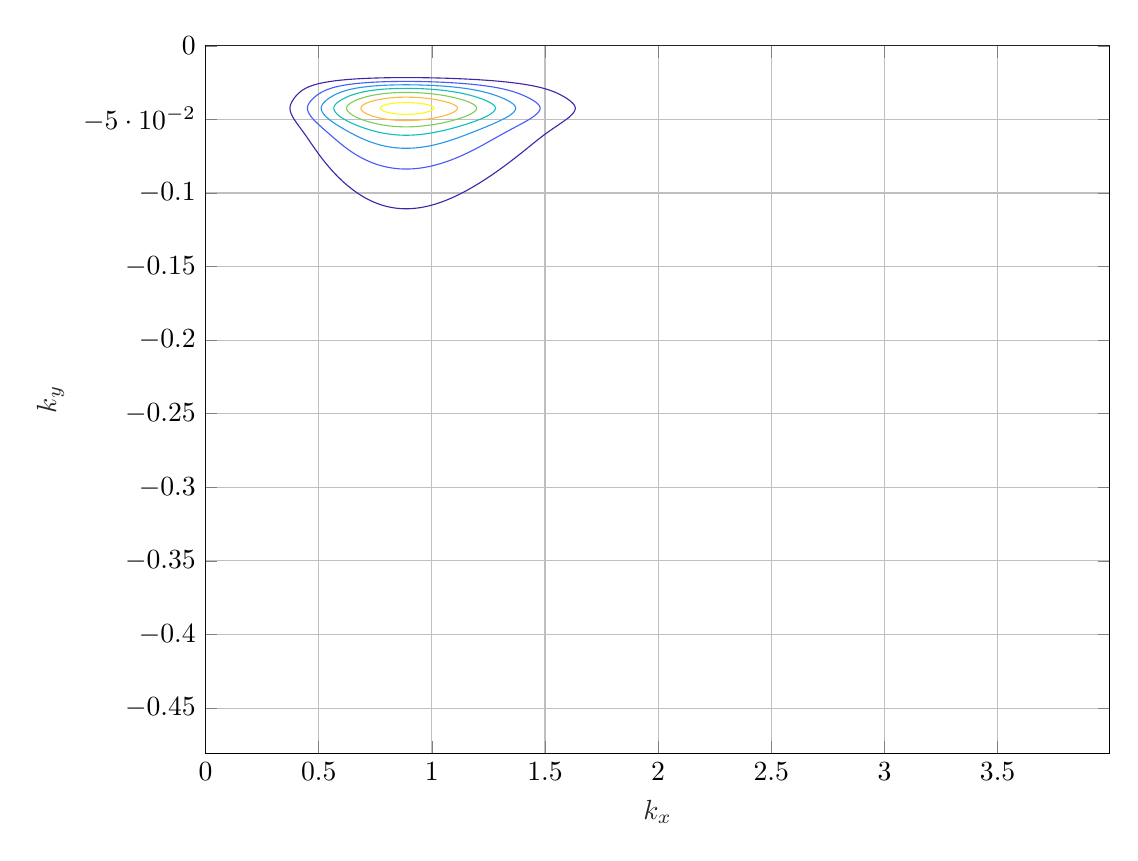
\begin{tikzpicture}

\begin{axis}[%
width=4.521in,
height=3.537in,
at={(0.758in,0.51in)},
scale only axis,
colormap={mymap}{[1pt] rgb(0pt)=(0.2422,0.1504,0.6603); rgb(1pt)=(0.2444,0.1534,0.6728); rgb(2pt)=(0.2464,0.1569,0.6847); rgb(3pt)=(0.2484,0.1607,0.6961); rgb(4pt)=(0.2503,0.1648,0.7071); rgb(5pt)=(0.2522,0.1689,0.7179); rgb(6pt)=(0.254,0.1732,0.7286); rgb(7pt)=(0.2558,0.1773,0.7393); rgb(8pt)=(0.2576,0.1814,0.7501); rgb(9pt)=(0.2594,0.1854,0.761); rgb(11pt)=(0.2628,0.1932,0.7828); rgb(12pt)=(0.2645,0.1972,0.7937); rgb(13pt)=(0.2661,0.2011,0.8043); rgb(14pt)=(0.2676,0.2052,0.8148); rgb(15pt)=(0.2691,0.2094,0.8249); rgb(16pt)=(0.2704,0.2138,0.8346); rgb(17pt)=(0.2717,0.2184,0.8439); rgb(18pt)=(0.2729,0.2231,0.8528); rgb(19pt)=(0.274,0.228,0.8612); rgb(20pt)=(0.2749,0.233,0.8692); rgb(21pt)=(0.2758,0.2382,0.8767); rgb(22pt)=(0.2766,0.2435,0.884); rgb(23pt)=(0.2774,0.2489,0.8908); rgb(24pt)=(0.2781,0.2543,0.8973); rgb(25pt)=(0.2788,0.2598,0.9035); rgb(26pt)=(0.2794,0.2653,0.9094); rgb(27pt)=(0.2798,0.2708,0.915); rgb(28pt)=(0.2802,0.2764,0.9204); rgb(29pt)=(0.2806,0.2819,0.9255); rgb(30pt)=(0.2809,0.2875,0.9305); rgb(31pt)=(0.2811,0.293,0.9352); rgb(32pt)=(0.2813,0.2985,0.9397); rgb(33pt)=(0.2814,0.304,0.9441); rgb(34pt)=(0.2814,0.3095,0.9483); rgb(35pt)=(0.2813,0.315,0.9524); rgb(36pt)=(0.2811,0.3204,0.9563); rgb(37pt)=(0.2809,0.3259,0.96); rgb(38pt)=(0.2807,0.3313,0.9636); rgb(39pt)=(0.2803,0.3367,0.967); rgb(40pt)=(0.2798,0.3421,0.9702); rgb(41pt)=(0.2791,0.3475,0.9733); rgb(42pt)=(0.2784,0.3529,0.9763); rgb(43pt)=(0.2776,0.3583,0.9791); rgb(44pt)=(0.2766,0.3638,0.9817); rgb(45pt)=(0.2754,0.3693,0.984); rgb(46pt)=(0.2741,0.3748,0.9862); rgb(47pt)=(0.2726,0.3804,0.9881); rgb(48pt)=(0.271,0.386,0.9898); rgb(49pt)=(0.2691,0.3916,0.9912); rgb(50pt)=(0.267,0.3973,0.9924); rgb(51pt)=(0.2647,0.403,0.9935); rgb(52pt)=(0.2621,0.4088,0.9946); rgb(53pt)=(0.2591,0.4145,0.9955); rgb(54pt)=(0.2556,0.4203,0.9965); rgb(55pt)=(0.2517,0.4261,0.9974); rgb(56pt)=(0.2473,0.4319,0.9983); rgb(57pt)=(0.2424,0.4378,0.9991); rgb(58pt)=(0.2369,0.4437,0.9996); rgb(59pt)=(0.2311,0.4497,0.9995); rgb(60pt)=(0.225,0.4559,0.9985); rgb(61pt)=(0.2189,0.462,0.9968); rgb(62pt)=(0.2128,0.4682,0.9948); rgb(63pt)=(0.2066,0.4743,0.9926); rgb(64pt)=(0.2006,0.4803,0.9906); rgb(65pt)=(0.195,0.4861,0.9887); rgb(66pt)=(0.1903,0.4919,0.9867); rgb(67pt)=(0.1869,0.4975,0.9844); rgb(68pt)=(0.1847,0.503,0.9819); rgb(69pt)=(0.1831,0.5084,0.9793); rgb(70pt)=(0.1818,0.5138,0.9766); rgb(71pt)=(0.1806,0.5191,0.9738); rgb(72pt)=(0.1795,0.5244,0.9709); rgb(73pt)=(0.1785,0.5296,0.9677); rgb(74pt)=(0.1778,0.5349,0.9641); rgb(75pt)=(0.1773,0.5401,0.9602); rgb(76pt)=(0.1768,0.5452,0.956); rgb(77pt)=(0.1764,0.5504,0.9516); rgb(78pt)=(0.1755,0.5554,0.9473); rgb(79pt)=(0.174,0.5605,0.9432); rgb(80pt)=(0.1716,0.5655,0.9393); rgb(81pt)=(0.1686,0.5705,0.9357); rgb(82pt)=(0.1649,0.5755,0.9323); rgb(83pt)=(0.161,0.5805,0.9289); rgb(84pt)=(0.1573,0.5854,0.9254); rgb(85pt)=(0.154,0.5902,0.9218); rgb(86pt)=(0.1513,0.595,0.9182); rgb(87pt)=(0.1492,0.5997,0.9147); rgb(88pt)=(0.1475,0.6043,0.9113); rgb(89pt)=(0.1461,0.6089,0.908); rgb(90pt)=(0.1446,0.6135,0.905); rgb(91pt)=(0.1429,0.618,0.9022); rgb(92pt)=(0.1408,0.6226,0.8998); rgb(93pt)=(0.1383,0.6272,0.8975); rgb(94pt)=(0.1354,0.6317,0.8953); rgb(95pt)=(0.1321,0.6363,0.8932); rgb(96pt)=(0.1288,0.6408,0.891); rgb(97pt)=(0.1253,0.6453,0.8887); rgb(98pt)=(0.1219,0.6497,0.8862); rgb(99pt)=(0.1185,0.6541,0.8834); rgb(100pt)=(0.1152,0.6584,0.8804); rgb(101pt)=(0.1119,0.6627,0.877); rgb(102pt)=(0.1085,0.6669,0.8734); rgb(103pt)=(0.1048,0.671,0.8695); rgb(104pt)=(0.1009,0.675,0.8653); rgb(105pt)=(0.0964,0.6789,0.8609); rgb(106pt)=(0.0914,0.6828,0.8562); rgb(107pt)=(0.0855,0.6865,0.8513); rgb(108pt)=(0.0789,0.6902,0.8462); rgb(109pt)=(0.0713,0.6938,0.8409); rgb(110pt)=(0.0628,0.6972,0.8355); rgb(111pt)=(0.0535,0.7006,0.8299); rgb(112pt)=(0.0433,0.7039,0.8242); rgb(113pt)=(0.0328,0.7071,0.8183); rgb(114pt)=(0.0234,0.7103,0.8124); rgb(115pt)=(0.0155,0.7133,0.8064); rgb(116pt)=(0.0091,0.7163,0.8003); rgb(117pt)=(0.0046,0.7192,0.7941); rgb(118pt)=(0.0019,0.722,0.7878); rgb(119pt)=(0.0009,0.7248,0.7815); rgb(120pt)=(0.0018,0.7275,0.7752); rgb(121pt)=(0.0046,0.7301,0.7688); rgb(122pt)=(0.0094,0.7327,0.7623); rgb(123pt)=(0.0162,0.7352,0.7558); rgb(124pt)=(0.0253,0.7376,0.7492); rgb(125pt)=(0.0369,0.74,0.7426); rgb(126pt)=(0.0504,0.7423,0.7359); rgb(127pt)=(0.0638,0.7446,0.7292); rgb(128pt)=(0.077,0.7468,0.7224); rgb(129pt)=(0.0899,0.7489,0.7156); rgb(130pt)=(0.1023,0.751,0.7088); rgb(131pt)=(0.1141,0.7531,0.7019); rgb(132pt)=(0.1252,0.7552,0.695); rgb(133pt)=(0.1354,0.7572,0.6881); rgb(134pt)=(0.1448,0.7593,0.6812); rgb(135pt)=(0.1532,0.7614,0.6741); rgb(136pt)=(0.1609,0.7635,0.6671); rgb(137pt)=(0.1678,0.7656,0.6599); rgb(138pt)=(0.1741,0.7678,0.6527); rgb(139pt)=(0.1799,0.7699,0.6454); rgb(140pt)=(0.1853,0.7721,0.6379); rgb(141pt)=(0.1905,0.7743,0.6303); rgb(142pt)=(0.1954,0.7765,0.6225); rgb(143pt)=(0.2003,0.7787,0.6146); rgb(144pt)=(0.2061,0.7808,0.6065); rgb(145pt)=(0.2118,0.7828,0.5983); rgb(146pt)=(0.2178,0.7849,0.5899); rgb(147pt)=(0.2244,0.7869,0.5813); rgb(148pt)=(0.2318,0.7887,0.5725); rgb(149pt)=(0.2401,0.7905,0.5636); rgb(150pt)=(0.2491,0.7922,0.5546); rgb(151pt)=(0.2589,0.7937,0.5454); rgb(152pt)=(0.2695,0.7951,0.536); rgb(153pt)=(0.2809,0.7964,0.5266); rgb(154pt)=(0.2929,0.7975,0.517); rgb(155pt)=(0.3052,0.7985,0.5074); rgb(156pt)=(0.3176,0.7994,0.4975); rgb(157pt)=(0.3301,0.8002,0.4876); rgb(158pt)=(0.3424,0.8009,0.4774); rgb(159pt)=(0.3548,0.8016,0.4669); rgb(160pt)=(0.3671,0.8021,0.4563); rgb(161pt)=(0.3795,0.8026,0.4454); rgb(162pt)=(0.3921,0.8029,0.4344); rgb(163pt)=(0.405,0.8031,0.4233); rgb(164pt)=(0.4184,0.803,0.4122); rgb(165pt)=(0.4322,0.8028,0.4013); rgb(166pt)=(0.4463,0.8024,0.3904); rgb(167pt)=(0.4608,0.8018,0.3797); rgb(168pt)=(0.4753,0.8011,0.3691); rgb(169pt)=(0.4899,0.8002,0.3586); rgb(170pt)=(0.5044,0.7993,0.348); rgb(171pt)=(0.5187,0.7982,0.3374); rgb(172pt)=(0.5329,0.797,0.3267); rgb(173pt)=(0.547,0.7957,0.3159); rgb(175pt)=(0.5748,0.7929,0.2941); rgb(176pt)=(0.5886,0.7913,0.2833); rgb(177pt)=(0.6024,0.7896,0.2726); rgb(178pt)=(0.6161,0.7878,0.2622); rgb(179pt)=(0.6297,0.7859,0.2521); rgb(180pt)=(0.6433,0.7839,0.2423); rgb(181pt)=(0.6567,0.7818,0.2329); rgb(182pt)=(0.6701,0.7796,0.2239); rgb(183pt)=(0.6833,0.7773,0.2155); rgb(184pt)=(0.6963,0.775,0.2075); rgb(185pt)=(0.7091,0.7727,0.1998); rgb(186pt)=(0.7218,0.7703,0.1924); rgb(187pt)=(0.7344,0.7679,0.1852); rgb(188pt)=(0.7468,0.7654,0.1782); rgb(189pt)=(0.759,0.7629,0.1717); rgb(190pt)=(0.771,0.7604,0.1658); rgb(191pt)=(0.7829,0.7579,0.1608); rgb(192pt)=(0.7945,0.7554,0.157); rgb(193pt)=(0.806,0.7529,0.1546); rgb(194pt)=(0.8172,0.7505,0.1535); rgb(195pt)=(0.8281,0.7481,0.1536); rgb(196pt)=(0.8389,0.7457,0.1546); rgb(197pt)=(0.8495,0.7435,0.1564); rgb(198pt)=(0.86,0.7413,0.1587); rgb(199pt)=(0.8703,0.7392,0.1615); rgb(200pt)=(0.8804,0.7372,0.165); rgb(201pt)=(0.8903,0.7353,0.1695); rgb(202pt)=(0.9,0.7336,0.1749); rgb(203pt)=(0.9093,0.7321,0.1815); rgb(204pt)=(0.9184,0.7308,0.189); rgb(205pt)=(0.9272,0.7298,0.1973); rgb(206pt)=(0.9357,0.729,0.2061); rgb(207pt)=(0.944,0.7285,0.2151); rgb(208pt)=(0.9523,0.7284,0.2237); rgb(209pt)=(0.9606,0.7285,0.2312); rgb(210pt)=(0.9689,0.7292,0.2373); rgb(211pt)=(0.977,0.7304,0.2418); rgb(212pt)=(0.9842,0.733,0.2446); rgb(213pt)=(0.99,0.7365,0.2429); rgb(214pt)=(0.9946,0.7407,0.2394); rgb(215pt)=(0.9966,0.7458,0.2351); rgb(216pt)=(0.9971,0.7513,0.2309); rgb(217pt)=(0.9972,0.7569,0.2267); rgb(218pt)=(0.9971,0.7626,0.2224); rgb(219pt)=(0.9969,0.7683,0.2181); rgb(220pt)=(0.9966,0.774,0.2138); rgb(221pt)=(0.9962,0.7798,0.2095); rgb(222pt)=(0.9957,0.7856,0.2053); rgb(223pt)=(0.9949,0.7915,0.2012); rgb(224pt)=(0.9938,0.7974,0.1974); rgb(225pt)=(0.9923,0.8034,0.1939); rgb(226pt)=(0.9906,0.8095,0.1906); rgb(227pt)=(0.9885,0.8156,0.1875); rgb(228pt)=(0.9861,0.8218,0.1846); rgb(229pt)=(0.9835,0.828,0.1817); rgb(230pt)=(0.9807,0.8342,0.1787); rgb(231pt)=(0.9778,0.8404,0.1757); rgb(232pt)=(0.9748,0.8467,0.1726); rgb(233pt)=(0.972,0.8529,0.1695); rgb(234pt)=(0.9694,0.8591,0.1665); rgb(235pt)=(0.9671,0.8654,0.1636); rgb(236pt)=(0.9651,0.8716,0.1608); rgb(237pt)=(0.9634,0.8778,0.1582); rgb(238pt)=(0.9619,0.884,0.1557); rgb(239pt)=(0.9608,0.8902,0.1532); rgb(240pt)=(0.9601,0.8963,0.1507); rgb(241pt)=(0.9596,0.9023,0.148); rgb(242pt)=(0.9595,0.9084,0.145); rgb(243pt)=(0.9597,0.9143,0.1418); rgb(244pt)=(0.9601,0.9203,0.1382); rgb(245pt)=(0.9608,0.9262,0.1344); rgb(246pt)=(0.9618,0.932,0.1304); rgb(247pt)=(0.9629,0.9379,0.1261); rgb(248pt)=(0.9642,0.9437,0.1216); rgb(249pt)=(0.9657,0.9494,0.1168); rgb(250pt)=(0.9674,0.9552,0.1116); rgb(251pt)=(0.9692,0.9609,0.1061); rgb(252pt)=(0.9711,0.9667,0.1001); rgb(253pt)=(0.973,0.9724,0.0938); rgb(254pt)=(0.9749,0.9782,0.0872); rgb(255pt)=(0.9769,0.9839,0.0805)},
xmin=0,
xmax=3.99549341800437,
xlabel style={font=\color{white!15!black}},
xlabel={$k_{x}$},
ymin=-0.480677883608269,
ymax=0,
ylabel style={font=\color{white!15!black}},
ylabel={$k_{y}$},
axis background/.style={fill=white},
xmajorgrids,
ymajorgrids
]
\addplot[contour prepared, contour prepared format=matlab, contour/labels=false] table[row sep=crcr] {%
%
0.005	615\\
0.755938347711432	-0.0218708335796425\\
0.760918854415919	-0.0218479569185073\\
0.767758540070646	-0.0218186272294896\\
0.774628828345752	-0.0217912719866442\\
0.781529719241237	-0.0217658417205903\\
0.788461212757101	-0.0217422906843998\\
0.795423308893345	-0.0217205767092487\\
0.802416007649967	-0.0217006610720749\\
0.809439309026969	-0.0216825083746312\\
0.816493213024349	-0.0216660864333786\\
0.823577719642109	-0.021651366179716\\
0.830692828880248	-0.0216383215700935\\
0.837838540738765	-0.0216269295056007\\
0.845014855217662	-0.0216171697606667\\
0.852221772316938	-0.0216090249205504\\
0.859459292036593	-0.0216024803273369\\
0.866727414376628	-0.0215975240341977\\
0.874026139337041	-0.021594146767705\\
0.881355466917834	-0.0215923418980287\\
0.888715397119005	-0.0215921054168763\\
0.896105929940556	-0.0215934359230722\\
0.903527065382485	-0.0215963346157018\\
0.910978803444794	-0.0216008052947815\\
0.918461144127482	-0.0216068543694459\\
0.925974087430549	-0.0216144908736745\\
0.933517633353995	-0.0216237264896141\\
0.94109178189782	-0.0216345755785838\\
0.948696533062024	-0.0216470552198822\\
0.956331886846607	-0.0216611852575496\\
0.96399784325157	-0.021676988355272\\
0.971694402276911	-0.0216944900596498\\
0.979421563922632	-0.0217137188720867\\
0.987179328188732	-0.0217347063295973\\
0.99496769507521	-0.0217574870948656\\
1.00278666458207	-0.0217820990559317\\
1.01063623670931	-0.0218085834359246\\
1.01851641145692	-0.0218369849133062\\
1.02642718882492	-0.0218673517531384\\
1.02728862027772	-0.0218708335796425\\
1.03436856881329	-0.0218981486038276\\
1.04234055142204	-0.0219307136011124\\
1.05034313665118	-0.0219652946102578\\
1.05837632450069	-0.0220019522727279\\
1.06644011497058	-0.0220407514166793\\
1.07453450806085	-0.0220817612566351\\
1.0826595037715	-0.022125055608514\\
1.09081510210252	-0.0221707131209914\\
1.09900130305393	-0.0222188175242522\\
1.10721810662572	-0.0222694578972834\\
1.1079271275333	-0.0222739741026576\\
1.11546551281788	-0.0223204123449869\\
1.12374352163043	-0.0223737537655685\\
1.13205213306335	-0.0224297986015511\\
1.14039134711665	-0.0224886550207235\\
1.14876116379033	-0.0225504378686066\\
1.15716158308439	-0.0226152690577291\\
1.16529037980338	-0.0226807962742846\\
1.16559260499883	-0.0226831776596654\\
1.17405422953365	-0.0227516183126857\\
1.18254645668885	-0.0228233798709646\\
1.19106928646443	-0.0228986107549261\\
1.19962271886038	-0.0229774684851165\\
1.20820675387672	-0.0230601202527463\\
1.2113508493998	-0.0230913000945237\\
1.21682139151343	-0.023144878514254\\
1.22546663177053	-0.0232326079368156\\
1.234142474648	-0.0233245506885638\\
1.24284892014585	-0.0234209120938217\\
1.25019337133736	-0.0235054855633748\\
1.25158596826408	-0.0235214644829499\\
1.26035361900269	-0.0236244578671368\\
1.26915187236168	-0.0237324271945599\\
1.27798072834105	-0.0238456271537823\\
1.28383407049896	-0.0239233526808379\\
1.2868401869408	-0.0239634711799871\\
1.29573024816092	-0.0240853572347932\\
1.30465091200143	-0.0242132117234233\\
1.31344293415244	-0.0243449014469129\\
1.31360217846231	-0.0243473172677454\\
1.32258404754357	-0.0244859780442554\\
1.33159651924522	-0.0246315240693008\\
1.33982131536433	-0.0247701318616\\
1.34063959356724	-0.0247842030198277\\
1.34971327050964	-0.0249431888941112\\
1.35881755007242	-0.0251102015932699\\
1.36351333381447	-0.0251990439248992\\
1.36795243225558	-0.0252853561445905\\
1.37711791705911	-0.0254690956422432\\
1.38489438952795	-0.0256316376368103\\
1.38631400448303	-0.0256623232022544\\
1.39554069452733	-0.0258657548095284\\
1.40430012903311	-0.0260679129973334\\
1.404797987192	-0.0260798659214223\\
1.41408588247706	-0.0263064825059535\\
1.42199302765399	-0.0265078700064685\\
1.42340438038249	-0.0265454730052639\\
1.4327534809083	-0.0267993974235814\\
1.43816847889269	-0.0269515086642157\\
1.44213318405449	-0.0270686213482722\\
1.45154348982107	-0.027354724954175\\
1.4529679290991	-0.0273988289705748\\
1.46098439820801	-0.0276610826523631\\
1.46658810863077	-0.027849830925546\\
1.47045590921534	-0.0279879920401411\\
1.47909801427682	-0.0283045145291292\\
1.47995802284305	-0.0283380253257745\\
1.48949073909114	-0.0287155881931983\\
1.4906648653855	-0.0287628797813244\\
1.4990540579596	-0.0291235268764456\\
1.50137378821029	-0.0292249266821316\\
1.50864797944845	-0.0295649721066249\\
1.51130122571058	-0.0296906552315508\\
1.51827250355767	-0.0300442720410201\\
1.52053248581189	-0.030160065429582\\
1.52792763028728	-0.0305660549540969\\
1.52914130155664	-0.0306331572762252\\
1.53720438421852	-0.0311099307714804\\
1.53761335963726	-0.0311356730973489\\
1.54481920187105	-0.0315903859153477\\
1.54732969160762	-0.0317596863816333\\
1.5519973309855	-0.0320745227078269\\
1.55707662619836	-0.0324400613372494\\
1.55877905818227	-0.0325623411489182\\
1.56525140737708	-0.0330538412386215\\
1.56685416340948	-0.0331821952790673\\
1.57145771149733	-0.0335490229769367\\
1.57666230324098	-0.0339890915644283\\
1.57736234166022	-0.034047886363864\\
1.58309505986288	-0.0345504313994033\\
1.58650104569286	-0.03486599338784\\
1.58857789751986	-0.0350566580835546\\
1.5938695423279	-0.035566566416318\\
1.59637039076512	-0.0358208213921423\\
1.59895080407938	-0.0360801563976933\\
1.60381342777846	-0.0365974280276806\\
1.60627033845775	-0.0368760153905426\\
1.60843831477895	-0.03711838130628\\
1.61281384893536	-0.0376430162334913\\
1.61620088877077	-0.0380871508733661\\
1.61685412518648	-0.0381713328093147\\
1.6206242090547	-0.0387033310337501\\
1.62396930744422	-0.0392390109067974\\
1.62616204170416	-0.0396467788356241\\
1.62688640512822	-0.0397783724284569\\
1.62938402221197	-0.0403214155987283\\
1.63134788539712	-0.0408681404176117\\
1.63274947658685	-0.0414185468851071\\
1.63356314466305	-0.0419726350012145\\
1.63376691489158	-0.042530404765934\\
1.63334318277323	-0.0430918561792654\\
1.63227998436755	-0.0436569892412089\\
1.63067884902791	-0.0442258039517643\\
1.62861740695224	-0.0447983003109318\\
1.62616204170416	-0.0453597397468779\\
1.62609920919489	-0.0453744783187113\\
1.62323189875118	-0.0459543379751028\\
1.61992956634594	-0.0465378792801063\\
1.61620088877077	-0.0471247602877373\\
1.61619875743385	-0.0471251022337218\\
1.61219770763277	-0.0477160068359494\\
1.60780213930552	-0.0483105930867889\\
1.60627033845775	-0.0485052957187258\\
1.60313931976355	-0.0489088609862404\\
1.59817615817887	-0.049510810534304\\
1.59637039076512	-0.0497203968695551\\
1.59299555269274	-0.0501164417309796\\
1.5875677852954	-0.0507257545762672\\
1.58650104569286	-0.0508425108414429\\
1.58200670292482	-0.0513387490701667\\
1.57666230324098	-0.0519093930032816\\
1.57623439568554	-0.0519554252126783\\
1.57040541422009	-0.0525757830038019\\
1.56685416340948	-0.0529465522716895\\
1.56444304583573	-0.0531998224435376\\
1.55840784473733	-0.0538275435318852\\
1.55707662619836	-0.0539659182892671\\
1.55235805783457	-0.0544589462688448\\
1.54732969160762	-0.0549804212342966\\
1.54623913787107	-0.0550940306544164\\
1.54015041100038	-0.0557327966886001\\
1.53761335963726	-0.0559998376917894\\
1.53406154480569	-0.0563752443713957\\
1.52795451022657	-0.0570213737028034\\
1.52792763028728	-0.0570242689094148\\
1.52194548166784	-0.0576711846828231\\
1.51827250355767	-0.0580698868324593\\
1.51593372339703	-0.0583246773114548\\
1.50996350420012	-0.0589818515886985\\
1.50864797944845	-0.0591288524207096\\
1.5040659188261	-0.0596427075145542\\
1.4990540579596	-0.0602077683322201\\
1.49817456159958	-0.0603072450890219\\
1.49236701595952	-0.0609754643121017\\
1.48949073909114	-0.0613091624393078\\
1.48658482630316	-0.0616473651837934\\
1.48082422937032	-0.0623229477040971\\
1.47995802284305	-0.0624260685934561\\
1.47513310366752	-0.0630022118730129\\
1.47045590921534	-0.0635619739471087\\
1.46942923368344	-0.0636851576905407\\
1.46377729717028	-0.0643717851566804\\
1.46098439820801	-0.0647125051911031\\
1.45812520786654	-0.0650620942714322\\
1.45246489831529	-0.065756085034796\\
1.45154348982107	-0.0658700988251399\\
1.44683520901436	-0.0664537574467718\\
1.44213318405449	-0.0670349258974961\\
1.44116195244527	-0.0671551115073596\\
1.43550308734357	-0.0678601472165594\\
1.4327534809083	-0.0682023821374733\\
1.42981083393808	-0.0685688645743713\\
1.42407502421041	-0.0692812635807951\\
1.42340438038249	-0.0693649847575489\\
1.41833857130262	-0.069997344235831\\
1.41408588247706	-0.0705248190412798\\
1.41253431407418	-0.0707171065394788\\
1.40669911122905	-0.0714405504917387\\
1.404797987192	-0.0716759398703197\\
1.4008201471781	-0.0721676760926106\\
1.39554069452733	-0.0728157524030019\\
1.39486512101548	-0.0728984833420945\\
1.38888077355354	-0.0736329722401904\\
1.38631400448303	-0.073946529799332\\
1.38282688177112	-0.0743711427868983\\
1.37711791705911	-0.0750615875530988\\
1.37669111809474	-0.0751129949822182\\
1.37051639833701	-0.0758585288261501\\
1.36795243225558	-0.0761665562140715\\
1.3642618420513	-0.0766077443186941\\
1.35881755007242	-0.0772546849063036\\
1.3579206821124	-0.07736064145985\\
1.35152027119691	-0.078117220249618\\
1.34971327050964	-0.0783303149865896\\
1.3450421805219	-0.0788774806879979\\
1.34063959356724	-0.0793907065467796\\
1.33847249878895	-0.0796414227749899\\
1.33181412670334	-0.0804090465105939\\
1.33159651924522	-0.0804342097133059\\
1.32508890642974	-0.0811803518948099\\
1.32258404754357	-0.0814665502648136\\
1.31826568842489	-0.0819553389276379\\
1.31360217846231	-0.0824817005956845\\
1.31134361220257	-0.0827340076090779\\
1.30465091200143	-0.0834800322358954\\
1.30432135178006	-0.0835163579391299\\
1.29721128139619	-0.084302389917794\\
1.29573024816092	-0.0844660560844381\\
1.28999577228534	-0.08509210354507\\
1.2868401869408	-0.0854363452417795\\
1.28266862837003	-0.085885498820958\\
1.27798072834105	-0.0863901938531484\\
1.27522650754913	-0.0866825757454581\\
1.26915187236168	-0.0873277963459003\\
1.26766537102176	-0.0874833343185702\\
1.26035361900269	-0.0882492989704053\\
1.25998042116331	-0.0882877745402943\\
1.2521688525393	-0.0890958964106304\\
1.25158596826408	-0.0891563757347774\\
1.24422092324414	-0.0899076999295784\\
1.24284892014585	-0.0900480160708609\\
1.23612734695441	-0.0907231850971386\\
1.234142474648	-0.0909231918811428\\
1.22787996360161	-0.0915423519133107\\
1.22546663177053	-0.0917818540063116\\
1.21946943978761	-0.0923652003780948\\
1.21682139151343	-0.092623906621502\\
1.21088513922219	-0.0931917304914909\\
1.20820675387672	-0.093449207691584\\
1.20211497263092	-0.0940219422534991\\
1.19962271886038	-0.0942575693100975\\
1.19314522340055	-0.0948558356641192\\
1.19106928646443	-0.0950487579043785\\
1.18396034445934	-0.0956934107233514\\
1.18254645668885	-0.095822494295149\\
1.17454272092732	-0.0965346674311956\\
1.17405422953365	-0.0965784536028746\\
1.16559260499883	-0.0973179482011682\\
1.16486771478451	-0.0973796057876518\\
1.15716158308439	-0.0980406379595306\\
1.15490922584174	-0.09822822579272\\
1.14876116379033	-0.0987449094306291\\
1.14464241256238	-0.0990805274464002\\
1.14039134711665	-0.0994302645225806\\
1.13403606166461	-0.0999365107486924\\
1.13205213306335	-0.100096157491128\\
1.12374352163043	-0.100743438766621\\
1.12304505727275	-0.100796175699597\\
1.11546551281788	-0.101374930973523\\
1.11159839067759	-0.101659522299113\\
1.10721810662572	-0.10198570150127\\
1.09966950110391	-0.102526550547241\\
1.09900130305393	-0.102575020433874\\
1.09081510210252	-0.103148917611086\\
1.08712439387746	-0.103397260443981\\
1.0826595037715	-0.103701753325531\\
1.07453450806085	-0.104232435648417\\
1.07391031877814	-0.104271651989334\\
1.06644011497058	-0.104747833136484\\
1.05982203282569	-0.105149725183298\\
1.05837632450069	-0.105238845934741\\
1.05034313665118	-0.105713178369005\\
1.04466861421925	-0.106031480025874\\
1.04234055142204	-0.106164184569842\\
1.03436856881329	-0.10659712409609\\
1.02814041972617	-0.106916916517062\\
1.02642718882492	-0.107006404609464\\
1.01851641145692	-0.107398418143536\\
1.01063623670931	-0.107765060296052\\
1.00970239886518	-0.107806034656863\\
1.00278666458207	-0.108115210361388\\
0.99496769507521	-0.108441649890776\\
0.98834563468107	-0.108698834445275\\
0.987179328188732	-0.108745034857709\\
0.979421563922632	-0.109031036345694\\
0.971694402276911	-0.10929307232439\\
0.96399784325157	-0.109531572556817\\
0.96173704615804	-0.109595315882299\\
0.956331886846607	-0.109751082502401\\
0.948696533062024	-0.109948915896088\\
0.94109178189782	-0.110123642237814\\
0.933517633353995	-0.110275539362211\\
0.925974087430549	-0.11040484639501\\
0.919607977548308	-0.110495478967936\\
0.918461144127482	-0.110512210751347\\
0.910978803444794	-0.110599224517959\\
0.903527065382485	-0.110663533630943\\
0.896105929940556	-0.110705230283397\\
0.888715397119005	-0.110724369137194\\
0.881355466917834	-0.110720967440745\\
0.874026139337041	-0.110695005038643\\
0.866727414376628	-0.110646424273041\\
0.859459292036593	-0.110575129776213\\
0.853333744216628	-0.110495478967936\\
0.852221772316938	-0.110481374715864\\
0.845014855217662	-0.110367339537814\\
0.837838540738765	-0.110230694221838\\
0.830692828880248	-0.110071194945701\\
0.823577719642109	-0.109888558532997\\
0.816493213024349	-0.109682461577946\\
0.813810674841223	-0.109595315882299\\
0.809439309026969	-0.109456349831547\\
0.802416007649967	-0.109208978348974\\
0.795423308893345	-0.108937582832723\\
0.789798374283232	-0.108698834445275\\
0.788461212757101	-0.10864320673005\\
0.781529719241237	-0.108330838725324\\
0.774628828345752	-0.107993545648167\\
0.771063445868687	-0.107806034656863\\
0.767758540070646	-0.107635402319369\\
0.760918854415919	-0.107256777638349\\
0.755193275214789	-0.106916916517062\\
0.754109771381571	-0.106853710101818\\
0.747331290967602	-0.106433520437933\\
0.741257773249516	-0.106031480025874\\
0.740583413174013	-0.105987562295621\\
0.733866138000802	-0.105525281818341\\
0.728729186845149	-0.105149725183298\\
0.727179465447971	-0.105038137714001\\
0.720523395515518	-0.104532945058435\\
0.717261439908291	-0.104271651989334\\
0.713897928203445	-0.104006001181487\\
0.707303063511751	-0.103456772755007\\
0.706620457940267	-0.103397260443981\\
0.700738801440436	-0.102891103547292\\
0.696711052271481	-0.102526550547241\\
0.6942051419895	-0.102302546493851\\
0.687702085158943	-0.101692774184811\\
0.68736178554515	-0.101659522299113\\
0.681229630948765	-0.101067079167689\\
0.678549518173803	-0.100796175699597\\
0.674787779358966	-0.100420011694074\\
0.670158975449137	-0.0999365107486924\\
0.668376530389547	-0.0997522120254341\\
0.662148106592559	-0.0990805274464002\\
0.661995884040506	-0.0990642683413111\\
0.655645840311844	-0.0983602294799441\\
0.654500546192145	-0.09822822579272\\
0.649326399203562	-0.0976368846284039\\
0.647158891747097	-0.0973796057876518\\
0.643037560715659	-0.0968942394455495\\
0.640093975100417	-0.0965346674311956\\
0.636779324848135	-0.0961326947677084\\
0.633282621629158	-0.0956934107233514\\
0.63055169160099	-0.0953526022632597\\
0.626704377262525	-0.0948558356641192\\
0.624354660974223	-0.0945542646891851\\
0.620341156083061	-0.0940219422534991\\
0.618188232967837	-0.0937379359683293\\
0.614176941329163	-0.0931917304914909\\
0.612052407581829	-0.09290382108896\\
0.608197530688152	-0.0923652003780948\\
0.6059471848162	-0.0920520758298827\\
0.602390318494937	-0.0915423519133107\\
0.59987256467095	-0.0911828063170614\\
0.596744108815605	-0.0907231850971386\\
0.59382854714608	-0.0902960684217547\\
0.591248954479506	-0.0899076999295784\\
0.587815132241588	-0.0893918670160067\\
0.585896017989385	-0.0890958964106304\\
0.581832319957476	-0.0884701551094348\\
0.580677450933755	-0.0882877745402943\\
0.575880110293743	-0.087530832902213\\
0.575586289084977	-0.0874833343185702\\
0.570617312509286	-0.0866825757454581\\
0.569958503250389	-0.0865765557394078\\
0.565763012853964	-0.085885498820958\\
0.564067498827413	-0.0856060656971499\\
0.561017661720752	-0.08509210354507\\
0.558207097024817	-0.0846178682596958\\
0.556376846020225	-0.084302389917794\\
0.552377297842601	-0.0836116444127438\\
0.551836693206074	-0.0835163579391299\\
0.547391905148615	-0.0827340076090779\\
0.546578101280763	-0.0825907465354429\\
0.543037991069677	-0.0819553389276379\\
0.540809507339304	-0.0815539704775669\\
0.53877305753733	-0.0811803518948099\\
0.535071516018224	-0.0804984239135297\\
0.534594807421209	-0.0804090465105939\\
0.530495526625574	-0.0796414227749899\\
0.529364127317524	-0.0794290461698929\\
0.526474135809923	-0.0788774806879979\\
0.523687341237202	-0.0783426354941249\\
0.522531107490831	-0.078117220249618\\
0.518660910800871	-0.07736064145985\\
0.51804115777726	-0.0772395026670398\\
0.514856409914316	-0.0766077443186941\\
0.512425576937697	-0.0761222344998128\\
0.511123451043303	-0.0758585288261501\\
0.507455865538003	-0.0751129949822182\\
0.506840598718512	-0.0749879581679379\\
0.503844538748665	-0.0743711427868983\\
0.501286223119707	-0.0738403601852374\\
0.500298651264284	-0.0736329722401904\\
0.496806679283428	-0.0728984833420945\\
0.495762450141281	-0.0726784439845321\\
0.493365588960508	-0.0721676760926106\\
0.490269279783234	-0.0715025261103268\\
0.489983761720597	-0.0714405504917387\\
0.486638306909718	-0.0707171065394788\\
0.484806712045567	-0.0703187335396727\\
0.483343166031317	-0.069997344235831\\
0.480091126931507	-0.0692812635807951\\
0.479374746928278	-0.0691239679520586\\
0.476868886084988	-0.0685688645743713\\
0.473973384431368	-0.067923318744129\\
0.473692323002892	-0.0678601472165594\\
0.470531854493427	-0.0671551115073596\\
0.468602624554837	-0.0667234726231281\\
0.467406110303056	-0.0664537574467718\\
0.464301084027397	-0.065756085034796\\
0.463262467298686	-0.0655239849900916\\
0.461209937024485	-0.0650620942714322\\
0.458144666970102	-0.0643717851566804\\
0.457952912662914	-0.0643292008397682\\
0.455071853838044	-0.0636851576905407\\
0.452673960647521	-0.0631491439448016\\
0.452020597818828	-0.0630022118730129\\
0.448961834385142	-0.0623229477040971\\
0.447425611252506	-0.0619841626101747\\
0.445907239963858	-0.0616473651837934\\
0.442854646998706	-0.0609754643121017\\
0.442207864477871	-0.0608352581161402\\
0.43978590065716	-0.0603072450890219\\
0.437020720323615	-0.0597066829481266\\
0.436727698633189	-0.0596427075145542\\
0.433644894370869	-0.0589818515886985\\
0.431864178789738	-0.0586024975584883\\
0.430566836686426	-0.0583246773114548\\
0.427486227099716	-0.0576711846828231\\
0.42673823987624	-0.0575146017163532\\
0.424394172110537	-0.0570213737028034\\
0.421642903583122	-0.0564430784799719\\
0.421321678311846	-0.0563752443713957\\
0.418237693494482	-0.0557327966886001\\
0.416578169910382	-0.0553870516102278\\
0.415177850463938	-0.0550940306544164\\
0.412144288649819	-0.0544589462688448\\
0.411544038858022	-0.0543337078487372\\
0.40912730899425	-0.0538275435318852\\
0.40654051042604	-0.0532786564492382\\
0.406170095256216	-0.0531998224435376\\
0.403244082291703	-0.0525757830038019\\
0.401567584614438	-0.0522112731763696\\
0.400393009392483	-0.0519554252126783\\
0.397615958401038	-0.0513387490701667\\
0.396625261423215	-0.0511133752734446\\
0.394921563723999	-0.0507257545762672\\
0.392339912313594	-0.0501164417309796\\
0.39171354085237	-0.0499633964973879\\
0.389857150462452	-0.049510810534304\\
0.387517232806171	-0.0489088609862404\\
0.386832422901905	-0.0487231377160627\\
0.385303381340041	-0.0483105930867889\\
0.383249178938984	-0.0477160068359494\\
0.381981907571819	-0.047318017153108\\
0.381362218084077	-0.0471251022337218\\
0.379633806474977	-0.0465378792801063\\
0.378103932476678	-0.0459543379751028\\
0.377161994862112	-0.0455448326504166\\
0.376764287383266	-0.0453744783187113\\
0.375606665963726	-0.0447983003109318\\
0.374659919379542	-0.0442258039517643\\
0.373924575208816	-0.0436569892412089\\
0.373436286223755	-0.0430918561792654\\
0.373241681223504	-0.042530404765934\\
0.373335265598294	-0.0419726350012145\\
0.373708954231558	-0.0414185468851071\\
0.37435265491418	-0.0408681404176117\\
0.375254587005457	-0.0403214155987283\\
0.376401653163925	-0.0397783724284569\\
0.377161994862112	-0.0394789292204609\\
0.377762312601035	-0.0392390109067974\\
0.379311998828793	-0.0387033310337501\\
0.381058568396491	-0.0381713328093147\\
0.381981907571819	-0.0379160877283267\\
0.382961234616668	-0.0376430162334913\\
0.385006074350883	-0.03711838130628\\
0.386832422901905	-0.0366849873958929\\
0.387199419811489	-0.0365974280276806\\
0.38949193817004	-0.0360801563976933\\
0.39171354085237	-0.0356111606811582\\
0.39192420979558	-0.035566566416318\\
0.394441116155405	-0.0350566580835546\\
0.396625261423215	-0.0346398473084971\\
0.397093680304832	-0.0345504313994033\\
0.399844683256408	-0.034047886363864\\
0.401567584614438	-0.0337502093776363\\
0.402734584250726	-0.0335490229769367\\
0.405765572333602	-0.0330538412386215\\
0.40654051042604	-0.0329336244265221\\
0.408945957741041	-0.0325623411489182\\
0.411544038858022	-0.032186336167104\\
0.412322111262039	-0.0320745227078269\\
0.415900213271366	-0.0315903859153477\\
0.416578169910382	-0.031504113309545\\
0.419709509014287	-0.0311099307714804\\
0.421642903583122	-0.0308829001892226\\
0.423798425492091	-0.0306331572762252\\
0.42673823987624	-0.0303156287974584\\
0.428202031902794	-0.030160065429582\\
0.431864178789738	-0.0297972496793779\\
0.432960976910717	-0.0296906552315508\\
0.437020720323615	-0.02932258963936\\
0.438122392082891	-0.0292249266821316\\
0.442207864477871	-0.0288866013247884\\
0.443741102341567	-0.0287628797813244\\
0.447425611252506	-0.0284845779102733\\
0.44988120009478	-0.0283045145291292\\
0.452673960647521	-0.0281123103319128\\
0.456618057534587	-0.027849830925546\\
0.457952912662914	-0.0277661839195541\\
0.463262467298686	-0.0274440248156604\\
0.464029127457633	-0.0273988289705748\\
0.468602624554837	-0.0271438323697324\\
0.472203705425871	-0.0269515086642157\\
0.473973384431368	-0.026861740188442\\
0.479374746928278	-0.0265971958970046\\
0.481266266812638	-0.0265078700064685\\
0.484806712045567	-0.0263482241677479\\
0.490269279783234	-0.0261131192819959\\
0.491352807206171	-0.0260679129973334\\
0.495762450141281	-0.0258912432653967\\
0.501286223119707	-0.0256810320838739\\
0.502627375275194	-0.0256316376368103\\
0.506840598718512	-0.0254817276563904\\
0.512425576937697	-0.0252925835208492\\
0.515304983908811	-0.0251990439248992\\
0.51804115777726	-0.0251126250723588\\
0.523687341237202	-0.0249413190681204\\
0.529364127317524	-0.024778529677478\\
0.529665116757637	-0.0247701318616\\
0.535071516018224	-0.0246224071241428\\
0.540809507339304	-0.0244738787580051\\
0.546062576870555	-0.0243449014469129\\
0.546578101280763	-0.0243324190177055\\
0.552377297842601	-0.0241959665317556\\
0.558207097024817	-0.0240661118529822\\
0.564067498827413	-0.0239425069861289\\
0.565005163484916	-0.0239233526808379\\
0.569958503250389	-0.0238227201761071\\
0.575880110293743	-0.0237082620533524\\
0.581832319957476	-0.0235992491268377\\
0.587221284345304	-0.0235054855633748\\
0.587815132241588	-0.0234951254876482\\
0.59382854714608	-0.0233934357580327\\
0.59987256467095	-0.0232965469203439\\
0.6059471848162	-0.0232042253428065\\
0.612052407581829	-0.0231162515707885\\
0.613850639874028	-0.0230913000945237\\
0.618188232967837	-0.023030369827951\\
0.624354660974223	-0.0229477048061566\\
0.63055169160099	-0.0228689365593588\\
0.636779324848135	-0.022793887882555\\
0.643037560715659	-0.0227223921501997\\
0.646850267296592	-0.0226807962742846\\
0.649326399203562	-0.0226531760924003\\
0.655645840311844	-0.0225855933853236\\
0.661995884040506	-0.022521251976534\\
0.668376530389547	-0.0224600160049549\\
0.674787779358966	-0.0224017576920213\\
0.681229630948765	-0.0223463568716768\\
0.687702085158943	-0.0222937005533663\\
0.690243299705289	-0.0222739741026576\\
0.6942051419895	-0.0222421713949123\\
0.700738801440436	-0.0221923232493968\\
0.707303063511751	-0.0221450417180306\\
0.713897928203445	-0.0221002343300088\\
0.720523395515518	-0.0220578142939029\\
0.727179465447971	-0.0220177002013276\\
0.733866138000802	-0.0219798157516261\\
0.740583413174013	-0.0219440894962016\\
0.747331290967602	-0.021910454601226\\
0.754109771381571	-0.0218788486275647\\
0.755938347711432	-0.0218708335796425\\
0.01	477\\
0.804377221313069	-0.0243449014469129\\
0.809439309026969	-0.0243241307640515\\
0.816493213024349	-0.0242980172511584\\
0.823577719642109	-0.0242746096936781\\
0.830692828880248	-0.0242538666782013\\
0.837838540738765	-0.0242357514737661\\
0.845014855217662	-0.0242202319184805\\
0.852221772316938	-0.0242072803201208\\
0.859459292036593	-0.0241968733702583\\
0.866727414376628	-0.024188992071525\\
0.874026139337041	-0.0241836216776877\\
0.881355466917834	-0.0241807516462561\\
0.888715397119005	-0.0241803756034042\\
0.896105929940556	-0.0241824913210387\\
0.903527065382485	-0.0241871007058971\\
0.910978803444794	-0.0241942098006134\\
0.918461144127482	-0.0242038287967364\\
0.925974087430549	-0.0242159720597382\\
0.933517633353995	-0.0242306581661007\\
0.94109178189782	-0.0242479099526179\\
0.948696533062024	-0.0242677545781062\\
0.956331886846607	-0.0242902235977629\\
0.96399784325157	-0.0243153530504737\\
0.971694402276911	-0.0243431835594184\\
0.972131100348352	-0.0243449014469129\\
0.979421563922632	-0.0243733280118298\\
0.987179328188732	-0.0244062013454073\\
0.99496769507521	-0.0244418835949337\\
1.00278666458207	-0.0244804341056716\\
1.01063623670931	-0.0245219174467415\\
1.01851641145692	-0.0245664035994634\\
1.02642718882492	-0.024613968162965\\
1.03436856881329	-0.0246646925779392\\
1.04234055142204	-0.0247186643695181\\
1.04953495253661	-0.0247701318616\\
1.05034313665118	-0.0247759229226535\\
1.05837632450069	-0.0248361114081239\\
1.06644011497058	-0.02489981600778\\
1.07453450806085	-0.0249671503654559\\
1.0826595037715	-0.0250382356800511\\
1.09081510210252	-0.0251132010854041\\
1.09900130305393	-0.0251921840587207\\
1.09968842658144	-0.0251990439248992\\
1.10721810662572	-0.0252750302960606\\
1.11546551281788	-0.0253621518288204\\
1.12374352163043	-0.0254537403057765\\
1.13205213306335	-0.0255499706107239\\
1.13881292215278	-0.0256316376368103\\
1.14039134711665	-0.0256510507273152\\
1.14876116379033	-0.0257572550967641\\
1.15716158308439	-0.0258686995477288\\
1.16559260499883	-0.0259856065132561\\
1.171308382622	-0.0260679129973334\\
1.17405422953365	-0.0261084507477863\\
1.18254645668885	-0.0262377668227145\\
1.19106928646443	-0.0263733347069774\\
1.19917599767789	-0.0265078700064685\\
1.19962271886038	-0.0265155166481849\\
1.20820675387672	-0.0266659998675478\\
1.21682139151343	-0.0268237139776552\\
1.22353916340034	-0.0269515086642157\\
1.22546663177053	-0.0269895425814385\\
1.234142474648	-0.0271652662903012\\
1.24284892014585	-0.0273494350605541\\
1.24512467028638	-0.0273988289705748\\
1.25158596826408	-0.0275450593419182\\
1.26035361900269	-0.0277510483265346\\
1.26443314898441	-0.027849830925546\\
1.26915187236168	-0.0279694758481234\\
1.27798072834105	-0.0282006833157385\\
1.28183181814757	-0.0283045145291292\\
1.2868401869408	-0.0284464347647729\\
1.29573024816092	-0.0287067707673443\\
1.29760318111818	-0.0287628797813244\\
1.30465091200143	-0.0289854762682231\\
1.31198020516963	-0.0292249266821316\\
1.31360217846231	-0.0292809016329018\\
1.32258404754357	-0.0295977864223809\\
1.32515326590878	-0.0296906552315508\\
1.33159651924522	-0.029937124870737\\
1.3372748196482	-0.030160065429582\\
1.34063959356724	-0.0302999476876293\\
1.34847269576132	-0.0306331572762252\\
1.34971327050964	-0.0306890290140477\\
1.35881755007242	-0.0311073156414761\\
1.35887361647227	-0.0311099307714804\\
1.36795243225558	-0.0315581892616901\\
1.36859375013575	-0.0315903859153477\\
1.37711791705911	-0.0320428027434456\\
1.37770710432257	-0.0320745227078269\\
1.38629305500815	-0.0325623411489182\\
1.38631400448303	-0.0325635917600528\\
1.39443798239201	-0.0330538412386215\\
1.39554069452733	-0.0331237790075846\\
1.40218594691251	-0.0335490229769367\\
1.404797987192	-0.0337244544249736\\
1.4095792864592	-0.034047886363864\\
1.41408588247706	-0.0343676234018784\\
1.41664840778149	-0.0345504313994033\\
1.42340438038249	-0.0350561157494074\\
1.42341159799414	-0.0350566580835546\\
1.42993816256341	-0.035566566416318\\
1.4327534809083	-0.0357983941677894\\
1.4361702294528	-0.0360801563976933\\
1.44209024096357	-0.0365974280276806\\
1.44213318405449	-0.0366013815811639\\
1.44775561024502	-0.03711838130628\\
1.45154348982107	-0.0374941010793685\\
1.45304951466801	-0.0376430162334913\\
1.45799315701663	-0.0381713328093147\\
1.46098439820801	-0.0385250154816472\\
1.46250269057418	-0.0387033310337501\\
1.46657003296878	-0.0392390109067974\\
1.47008453000994	-0.0397783724284569\\
1.47045590921534	-0.0398466049368106\\
1.47307525118449	-0.0403214155987283\\
1.47543434956648	-0.0408681404176117\\
1.47711801650055	-0.0414185468851071\\
1.47809543848012	-0.0419726350012145\\
1.47834021826929	-0.042530404765934\\
1.47783120839409	-0.0430918561792654\\
1.47655403712395	-0.0436569892412089\\
1.47463066699427	-0.0442258039517643\\
1.47215435158593	-0.0447983003109318\\
1.47045590921534	-0.0451231997331659\\
1.46915980423348	-0.0453744783187113\\
1.46567340952453	-0.0459543379751028\\
1.46165806676661	-0.0465378792801063\\
1.46098439820801	-0.0466264004715795\\
1.45721557147711	-0.0471251022337218\\
1.45229118407497	-0.0477160068359494\\
1.45154348982107	-0.0477996627393414\\
1.44699106789972	-0.0483105930867889\\
1.44213318405449	-0.0488184790177547\\
1.44126954673455	-0.0489088609862404\\
1.43522713516224	-0.049510810534304\\
1.4327534809083	-0.0497463903289186\\
1.42886020854464	-0.0501164417309796\\
1.42340438038249	-0.0506153033606723\\
1.42219207624339	-0.0507257545762672\\
1.41528845388748	-0.0513387490701667\\
1.41408588247706	-0.0514435722909148\\
1.40818073473732	-0.0519554252126783\\
1.404797987192	-0.052243909954019\\
1.4008799728383	-0.0525757830038019\\
1.39554069452733	-0.0530234573312205\\
1.39342067663213	-0.0531998224435376\\
1.38631400448303	-0.0537881799783341\\
1.3858343436145	-0.0538275435318852\\
1.3781674671552	-0.0544589462688448\\
1.37711791705911	-0.0545458226127651\\
1.37043153747169	-0.0550940306544164\\
1.36795243225558	-0.0552986906260129\\
1.36264002656672	-0.0557327966886001\\
1.35881755007242	-0.0560482331353964\\
1.35481172330048	-0.0563752443713957\\
1.34971327050964	-0.0567965753715615\\
1.34696190716407	-0.0570213737028034\\
1.34063959356724	-0.0575453052287244\\
1.33910241001668	-0.0576711846828231\\
1.33159651924522	-0.0582955294323516\\
1.33124172591043	-0.0583246773114548\\
1.32339510768376	-0.0589818515886985\\
1.32258404754357	-0.0590510097243626\\
1.31555730022327	-0.0596427075145542\\
1.31360217846231	-0.0598101811092427\\
1.30772315174896	-0.0603072450890219\\
1.30465091200143	-0.0605714819000934\\
1.29988966923131	-0.0609754643121017\\
1.29573024816092	-0.0613343840060109\\
1.29205156196097	-0.0616473651837934\\
1.2868401869408	-0.0620980753273685\\
1.28420150014653	-0.0623229477040971\\
1.27798072834105	-0.0628615097859137\\
1.27633036104792	-0.0630022118730129\\
1.26915187236168	-0.0636234615969501\\
1.26842745394948	-0.0636851576905407\\
1.26048146154921	-0.0643717851566804\\
1.26035361900269	-0.0643829970995432\\
1.2524812104185	-0.0650620942714322\\
1.25158596826408	-0.0651402408670187\\
1.24440755056038	-0.065756085034796\\
1.24284892014585	-0.0658912807559066\\
1.23624534369705	-0.0664537574467718\\
1.234142474648	-0.0666347134942917\\
1.22797855229069	-0.0671551115073596\\
1.22546663177053	-0.0673692095077424\\
1.21959023842266	-0.0678601472165594\\
1.21682139151343	-0.0680935345412937\\
1.21106251599034	-0.0685688645743713\\
1.20820675387672	-0.0688065614543625\\
1.202376455522	-0.0692812635807951\\
1.19962271886038	-0.0695072732207551\\
1.19351194065745	-0.069997344235831\\
1.19106928646443	-0.0701947586462383\\
1.18444747473268	-0.0707171065394788\\
1.18254645668885	-0.0708682025491186\\
1.17515993492823	-0.0714405504917387\\
1.17405422953365	-0.0715268721630858\\
1.16562427007291	-0.0721676760926106\\
1.16559260499883	-0.072170101368872\\
1.15716158308439	-0.0727998888549238\\
1.1558025791979	-0.0728984833420945\\
1.14876116379033	-0.07341355628924\\
1.14566822246491	-0.0736329722401904\\
1.14039134711665	-0.0740104991128655\\
1.13518605505927	-0.0743711427868983\\
1.13205213306335	-0.0745901841700147\\
1.12431647339254	-0.0751129949822182\\
1.12374352163043	-0.0751520726575404\\
1.11546551281788	-0.0756996845877829\\
1.11297713738834	-0.0758585288261501\\
1.10721810662572	-0.0762298792363737\\
1.10112796883184	-0.0766077443186941\\
1.09900130305393	-0.0767410937589243\\
1.09081510210252	-0.0772358941490573\\
1.08867039935287	-0.07736064145985\\
1.0826595037715	-0.0777143434458983\\
1.07550335332597	-0.078117220249618\\
1.07453450806085	-0.0781724299803268\\
1.06644011497058	-0.0786161041324867\\
1.06144179325742	-0.0788774806879979\\
1.05837632450069	-0.079039917202329\\
1.05034313665118	-0.079446662240167\\
1.04630317308328	-0.0796414227749899\\
1.04234055142204	-0.0798352141260099\\
1.03436856881329	-0.0802058209649157\\
1.02975425367427	-0.0804090465105939\\
1.02642718882492	-0.0805578628081773\\
1.01851641145692	-0.0808928785784077\\
1.01129192309817	-0.0811803518948099\\
1.01063623670931	-0.0812068795580805\\
1.00278666458207	-0.0815066065359406\\
0.99496769507521	-0.0817851431190709\\
0.989838953267046	-0.0819553389276379\\
0.987179328188732	-0.0820452259432822\\
0.979421563922632	-0.0822888975335707\\
0.971694402276911	-0.0825121506505094\\
0.96399784325157	-0.0827153514496693\\
0.963221998184426	-0.0827340076090779\\
0.956331886846607	-0.082903117227403\\
0.948696533062024	-0.0830714382139684\\
0.94109178189782	-0.0832200992143692\\
0.933517633353995	-0.0833493366163993\\
0.925974087430549	-0.0834593538734712\\
0.92127069463616	-0.0835163579391299\\
0.918461144127482	-0.0835512086980988\\
0.910978803444794	-0.0836251480662423\\
0.903527065382485	-0.0836797943063152\\
0.896105929940556	-0.0837152257587874\\
0.888715397119005	-0.0837314888722211\\
0.881355466917834	-0.08372859830334\\
0.874026139337041	-0.0837065369252194\\
0.866727414376628	-0.0836652557434893\\
0.859459292036593	-0.0836046737200599\\
0.852221772316938	-0.0835246775034803\\
0.851618010403983	-0.0835163579391299\\
0.845014855217662	-0.0834274422174631\\
0.837838540738765	-0.0833111813882576\\
0.830692828880248	-0.0831754759089378\\
0.823577719642109	-0.0830200848468113\\
0.816493213024349	-0.0828447330411542\\
0.812491267403402	-0.0827340076090779\\
0.809439309026969	-0.0826512621289409\\
0.802416007649967	-0.0824405030766882\\
0.795423308893345	-0.0822092756886489\\
0.788461212757101	-0.0819571689790159\\
0.788414473432498	-0.0819553389276379\\
0.781529719241237	-0.0816905927946798\\
0.774628828345752	-0.0814027953536016\\
0.769680408526579	-0.0811803518948099\\
0.767758540070646	-0.0810954058620311\\
0.760918854415919	-0.08077183223991\\
0.754109771381571	-0.0804258873958315\\
0.753797330473802	-0.0804090465105939\\
0.747331290967602	-0.0800657722262189\\
0.740583413174013	-0.0796829893874905\\
0.739889674237461	-0.0796414227749899\\
0.733866138000802	-0.0792855389770529\\
0.727372866057547	-0.0788774806879979\\
0.727179465447971	-0.0788654888762084\\
0.720523395515518	-0.0784315055680017\\
0.715967659361063	-0.078117220249618\\
0.713897928203445	-0.0779761817928272\\
0.707303063511751	-0.0775035110394896\\
0.705403862926302	-0.07736064145985\\
0.700738801440436	-0.077013613042942\\
0.695551252915864	-0.0766077443186941\\
0.6942051419895	-0.0765035434082858\\
0.687702085158943	-0.0759768731502241\\
0.686303425358596	-0.0758585288261501\\
0.681229630948765	-0.0754333337447613\\
0.67757563874983	-0.0751129949822182\\
0.674787779358966	-0.0748708224605715\\
0.669280220196376	-0.0743711427868983\\
0.668376530389547	-0.0742898724541303\\
0.661995884040506	-0.0736925161020876\\
0.661383609750909	-0.0736329722401904\\
0.655645840311844	-0.0730793696271315\\
0.65384276319976	-0.0728984833420945\\
0.649326399203562	-0.0724488558813378\\
0.646606314852163	-0.0721676760926106\\
0.643037560715659	-0.0718015227056221\\
0.639644714237953	-0.0714405504917387\\
0.636779324848135	-0.0711379499112949\\
0.632931430706761	-0.0707171065394788\\
0.63055169160099	-0.0704587667834171\\
0.626442509636065	-0.069997344235831\\
0.624354660974223	-0.0697646700716183\\
0.620156202684683	-0.0692812635807951\\
0.618188232967837	-0.0690564414045641\\
0.614052661679846	-0.0685688645743713\\
0.612052407581829	-0.068334962726956\\
0.60811368809465	-0.0678601472165594\\
0.6059471848162	-0.0676012280634873\\
0.602322531892546	-0.0671551115073596\\
0.59987256467095	-0.066856349723109\\
0.596663734884911	-0.0664537574467718\\
0.59382854714608	-0.0661015570354608\\
0.591123014736477	-0.065756085034796\\
0.587815132241588	-0.0653381859184013\\
0.585687186411763	-0.0650620942714322\\
0.581832319957476	-0.0645676580461501\\
0.58034411822141	-0.0643717851566804\\
0.575880110293743	-0.0637914491149447\\
0.57508271973218	-0.0636851576905407\\
0.569958503250389	-0.0630110466262941\\
0.569892958678732	-0.0630022118730129\\
0.564766235854214	-0.0623229477040971\\
0.564067498827413	-0.0622318007828213\\
0.559693076548791	-0.0616473651837934\\
0.558207097024817	-0.0614519649621689\\
0.55466684396607	-0.0609754643121017\\
0.552377297842601	-0.0606722925328753\\
0.549682360403837	-0.0603072450890219\\
0.546578101280763	-0.0598936486504748\\
0.54473590863206	-0.0596427075145542\\
0.540809507339304	-0.059116603410152\\
0.539825329554973	-0.0589818515886985\\
0.535071516018224	-0.0583413818405251\\
0.534950115119751	-0.0583246773114548\\
0.530107716667587	-0.0576711846828231\\
0.529364127317524	-0.0575723866018814\\
0.525302843479387	-0.0570213737028034\\
0.523687341237202	-0.0568051141950134\\
0.520540834177974	-0.0563752443713957\\
0.51804115777726	-0.0560376310507096\\
0.515828348784797	-0.0557327966886001\\
0.512425576937697	-0.0552682253878933\\
0.51117385567571	-0.0550940306544164\\
0.506840598718512	-0.0544945975913452\\
0.506587584940164	-0.0544589462688448\\
0.502074014458476	-0.0538275435318852\\
0.501286223119707	-0.0537173876424764\\
0.497649537982167	-0.0531998224435376\\
0.495762450141281	-0.0529296914058139\\
0.493330986482014	-0.0525757830038019\\
0.490269279783234	-0.0521251116813413\\
0.48913431318809	-0.0519554252126783\\
0.485073409872808	-0.0513387490701667\\
0.484806712045567	-0.0512975812763048\\
0.48115314359538	-0.0507257545762672\\
0.479374746928278	-0.0504385660548602\\
0.477404447920621	-0.0501164417309796\\
0.473973384431368	-0.0495326414754945\\
0.473846441923124	-0.049510810534304\\
0.470471763228318	-0.0489088609862404\\
0.468602624554837	-0.0485551904969067\\
0.467319814397737	-0.0483105930867889\\
0.464395000205959	-0.0477160068359494\\
0.463262467298686	-0.0474674159394559\\
0.461709255657238	-0.0471251022337218\\
0.459279668638239	-0.0465378792801063\\
0.457952912662914	-0.0461800560774934\\
0.457115857213614	-0.0459543379751028\\
0.455218483361123	-0.0453744783187113\\
0.453611959826929	-0.0447983003109318\\
0.452673960647521	-0.0443907474790607\\
0.452291704025539	-0.0442258039517643\\
0.451253886509983	-0.0436569892412089\\
0.450564746809795	-0.0430918561792654\\
0.450290093816114	-0.042530404765934\\
0.450422172789752	-0.0419726350012145\\
0.450949572916665	-0.0414185468851071\\
0.451858050701348	-0.0408681404176117\\
0.452673960647521	-0.0405165142841099\\
0.45312335178737	-0.0403214155987283\\
0.454715226944265	-0.0397783724284569\\
0.456627894713476	-0.0392390109067974\\
0.457952912662914	-0.0389162813701167\\
0.458827311297159	-0.0387033310337501\\
0.46128242252594	-0.0381713328093147\\
0.463262467298686	-0.0377838315717072\\
0.463985019358931	-0.0376430162334913\\
0.46689650279964	-0.03711838130628\\
0.468602624554837	-0.0368322621219538\\
0.470013406610849	-0.0365974280276806\\
0.473319725036751	-0.0360801563976933\\
0.473973384431368	-0.0359828172345266\\
0.476797151884768	-0.035566566416318\\
0.479374746928278	-0.0352065001180172\\
0.480460152635741	-0.0350566580835546\\
0.484303719109245	-0.0345504313994033\\
0.484806712045567	-0.0344869018407964\\
0.488332491604438	-0.034047886363864\\
0.490269279783234	-0.0338182027699262\\
0.492575625995173	-0.0335490229769367\\
0.495762450141281	-0.0331950026148191\\
0.497055922181604	-0.0330538412386215\\
0.501286223119707	-0.0326150034717936\\
0.501803966256058	-0.0325623411489182\\
0.506840598718512	-0.0320762088177678\\
0.506858452105071	-0.0320745227078269\\
0.512265442413182	-0.0315903859153477\\
0.512425576937697	-0.0315768336529142\\
0.51804115777726	-0.0311134749575014\\
0.518085221564965	-0.0311099307714804\\
0.523687341237202	-0.0306843459976574\\
0.524381058544938	-0.0306331572762252\\
0.529364127317524	-0.0302861165017486\\
0.531232887505667	-0.030160065429582\\
0.535071516018224	-0.0299157058257207\\
0.5387330742282	-0.0296906552315508\\
0.540809507339304	-0.0295701356340848\\
0.546578101280763	-0.0292472817563705\\
0.54698916971606	-0.0292249266821316\\
0.552377297842601	-0.0289476880029908\\
0.556126639787641	-0.0287628797813244\\
0.558207097024817	-0.028665664622949\\
0.564067498827413	-0.0284016574156753\\
0.566307163510067	-0.0283045145291292\\
0.569958503250389	-0.0281538965117911\\
0.575880110293743	-0.0279201192834963\\
0.577726562839175	-0.027849830925546\\
0.581832319957476	-0.027700630303487\\
0.587815132241588	-0.0274929431444599\\
0.590639088396924	-0.0273988289705748\\
0.59382854714608	-0.0272969214742301\\
0.59987256467095	-0.027111744659502\\
0.605377242887216	-0.0269515086642157\\
0.6059471848162	-0.0269355273365821\\
0.612052407581829	-0.0267697789185667\\
0.618188232967837	-0.0266118335765053\\
0.622419468527745	-0.0265078700064685\\
0.624354660974223	-0.0264618033824036\\
0.63055169160099	-0.0263198610841988\\
0.636779324848135	-0.0261846215416697\\
0.642437852311271	-0.0260679129973334\\
0.643037560715659	-0.0260558559037839\\
0.649326399203562	-0.0259338615280013\\
0.655645840311844	-0.0258176872330852\\
0.661995884040506	-0.0257070847117692\\
0.666546536336684	-0.0256316376368103\\
0.668376530389547	-0.0256018546049098\\
0.674787779358966	-0.0255018237078426\\
0.681229630948765	-0.0254066991929319\\
0.687702085158943	-0.0253162870527304\\
0.6942051419895	-0.0252304049025704\\
0.696696002396716	-0.0251990439248992\\
0.700738801440436	-0.0251486829140832\\
0.707303063511751	-0.0250710510201791\\
0.713897928203445	-0.0249974814404188\\
0.720523395515518	-0.0249278316713182\\
0.727179465447971	-0.0248619680478506\\
0.733866138000802	-0.0247997652914072\\
0.737240571756527	-0.0247701318616\\
0.740583413174013	-0.024740832988653\\
0.747331290967602	-0.0246850879957845\\
0.754109771381571	-0.0246327056477014\\
0.760918854415919	-0.02458358940612\\
0.767758540070646	-0.0245376493654878\\
0.774628828345752	-0.0244948019637623\\
0.781529719241237	-0.0244549697154524\\
0.788461212757101	-0.0244180809656648\\
0.795423308893345	-0.0243840696640063\\
0.802416007649967	-0.0243528751572922\\
0.804377221313069	-0.0243449014469129\\
0.015	385\\
0.862374478884527	-0.0265078700064685\\
0.866727414376628	-0.0265009439978092\\
0.874026139337041	-0.0264930586332131\\
0.881355466917834	-0.0264888445578721\\
0.888715397119005	-0.0264882924130797\\
0.896105929940556	-0.0264913989273198\\
0.903527065382485	-0.0264981669002606\\
0.910454690664743	-0.0265078700064685\\
0.910978803444794	-0.0265086128194804\\
0.918461144127482	-0.0265228827108389\\
0.925974087430549	-0.0265408973811391\\
0.933517633353995	-0.0265626843888053\\
0.94109178189782	-0.0265882776124843\\
0.948696533062024	-0.0266177173425921\\
0.956331886846607	-0.0266510503916272\\
0.96399784325157	-0.0266883302236906\\
0.971694402276911	-0.0267296171037368\\
0.979421563922632	-0.0267749782671628\\
0.987179328188732	-0.0268244881104336\\
0.99496769507521	-0.0268782284035327\\
1.00278666458207	-0.0269362885251246\\
1.00471101872177	-0.0269515086642157\\
1.01063623670931	-0.0269994470447589\\
1.01851641145692	-0.0270674126733939\\
1.02642718882492	-0.0271400814761863\\
1.03436856881329	-0.027217577877649\\
1.04234055142204	-0.0273000355980582\\
1.05034313665118	-0.0273875980553384\\
1.05132501096458	-0.0273988289705748\\
1.05837632450069	-0.0274818920412375\\
1.06644011497058	-0.0275819091695396\\
1.07453450806085	-0.0276876250696028\\
1.0826595037715	-0.0277992300254246\\
1.0861931251173	-0.027849830925546\\
1.09081510210252	-0.0279183508064654\\
1.09900130305393	-0.0280449870405962\\
1.10721810662572	-0.0281782992885598\\
1.11465210738672	-0.0283045145291292\\
1.11546551281788	-0.0283188714773901\\
1.12374352163043	-0.0284698171964547\\
1.13205213306335	-0.0286284130488899\\
1.13880660054791	-0.0287628797813244\\
1.14039134711665	-0.0287957964182241\\
1.14876116379033	-0.0289751594200613\\
1.15716158308439	-0.0291633721213546\\
1.15982363653798	-0.0292249266821316\\
1.16559260499883	-0.02936452129499\\
1.17405422953365	-0.0295772384694146\\
1.1784140957844	-0.0296906552315508\\
1.18254645668885	-0.0298033491721734\\
1.19106928646443	-0.0300437232169202\\
1.19506271379138	-0.030160065429582\\
1.19962271886038	-0.0302994859685905\\
1.20820675387672	-0.0305709711172835\\
1.21012172695174	-0.0306331572762252\\
1.21682139151343	-0.0308615749944324\\
1.22385962219135	-0.0311099307714804\\
1.22546663177053	-0.0311694198717714\\
1.234142474648	-0.0314988052647886\\
1.23649207550855	-0.0315903859153477\\
1.24284892014585	-0.0318501189032056\\
1.24819021497304	-0.0320745227078269\\
1.25158596826408	-0.0322238219121369\\
1.25909196107259	-0.0325623411489182\\
1.26035361900269	-0.032621775820498\\
1.26915187236168	-0.0330457915583518\\
1.26931580732268	-0.0330538412386215\\
1.27798072834105	-0.0334977136353848\\
1.27896229172345	-0.0335490229769367\\
1.2868401869408	-0.0339780289463958\\
1.28809969207308	-0.034047886363864\\
1.29573024816092	-0.0344884806414287\\
1.29678556953099	-0.0345504313994033\\
1.30465091200143	-0.0350312653945802\\
1.30506017521506	-0.0350566580835546\\
1.31295455562035	-0.035566566416318\\
1.31360217846231	-0.0356102714683972\\
1.32047998525662	-0.0360801563976933\\
1.32258404754357	-0.0362313474140305\\
1.32762541524641	-0.0365974280276806\\
1.33159651924522	-0.0369030844663435\\
1.33436962242692	-0.03711838130628\\
1.34063959356724	-0.037639815791378\\
1.34067782278246	-0.0376430162334913\\
1.34655026189983	-0.0381713328093147\\
1.34971327050964	-0.0384857597393504\\
1.35189550943872	-0.0387033310337501\\
1.35668041907834	-0.0392390109067974\\
1.35881755007242	-0.0395158993338494\\
1.3608467045638	-0.0397783724284569\\
1.36434249872442	-0.0403214155987283\\
1.36709122329858	-0.0408681404176117\\
1.36795243225558	-0.0411088456899586\\
1.36907139508196	-0.0414185468851071\\
1.37022932106513	-0.0419726350012145\\
1.37051930521114	-0.042530404765934\\
1.36991629466656	-0.0430918561792654\\
1.36840326362208	-0.0436569892412089\\
1.36795243225558	-0.0437702369803249\\
1.36615480536327	-0.0442258039517643\\
1.36326950432274	-0.0447983003109318\\
1.35974154199139	-0.0453744783187113\\
1.35881755007242	-0.0455044718123686\\
1.35562561184913	-0.0459543379751028\\
1.35090187570775	-0.0465378792801063\\
1.34971327050964	-0.0466704672374781\\
1.34562658591007	-0.0471251022337218\\
1.34063959356724	-0.0476302933285813\\
1.33978907386015	-0.0477160068359494\\
1.33345252697685	-0.0483105930867889\\
1.33159651924522	-0.0484744270413398\\
1.32663122046108	-0.0489088609862404\\
1.32258404754357	-0.0492451348139357\\
1.31935151969161	-0.049510810534304\\
1.31360217846231	-0.0499644271071239\\
1.31165068756033	-0.0501164417309796\\
1.30465091200143	-0.0506449308823759\\
1.30356475179091	-0.0507257545762672\\
1.29573024816092	-0.0512956650095121\\
1.29512835345407	-0.0513387490701667\\
1.2868401869408	-0.0519231626372319\\
1.28637452822788	-0.0519554252126783\\
1.27798072834105	-0.0525322039020256\\
1.27733442957315	-0.0525757830038019\\
1.26915187236168	-0.0531263066563777\\
1.26803700567458	-0.0531998224435376\\
1.26035361900269	-0.0537080623279168\\
1.25850864400026	-0.0538275435318852\\
1.25158596826408	-0.0542793700562188\\
1.24877279841501	-0.0544589462688448\\
1.24284892014585	-0.0548416025204458\\
1.23884961378699	-0.0550940306544164\\
1.234142474648	-0.0553957250415837\\
1.22875556189422	-0.0557327966886001\\
1.22546663177053	-0.0559423822488151\\
1.21850310021214	-0.0563752443713957\\
1.21682139151343	-0.0564819619811633\\
1.20820675387672	-0.0570149346863322\\
1.20810031515829	-0.0570213737028034\\
1.19962271886038	-0.0575462092716381\\
1.19754761057162	-0.0576711846828231\\
1.19106928646443	-0.0580710426081691\\
1.18684176107946	-0.0583246773114548\\
1.18254645668885	-0.0585890523005624\\
1.17597553768749	-0.0589818515886985\\
1.17405422953365	-0.0590997539393938\\
1.16559260499883	-0.0596043653577663\\
1.16493209646878	-0.0596427075145542\\
1.15716158308439	-0.0601061434734406\\
1.15367901010236	-0.0603072450890219\\
1.14876116379033	-0.0605990049415749\\
1.14220077984792	-0.0609754643121017\\
1.14039134711665	-0.0610821108377326\\
1.13205213306335	-0.061558520217124\\
1.13044619560434	-0.0616473651837934\\
1.12374352163043	-0.0620282447905176\\
1.11836147864524	-0.0623229477040971\\
1.11546551281788	-0.0624857195939338\\
1.10721810662572	-0.0629328839289893\\
1.1058944300064	-0.0630022118730129\\
1.09900130305393	-0.0633727077833444\\
1.09294124472147	-0.0636851576905407\\
1.09081510210252	-0.0637975566063399\\
1.0826595037715	-0.0642126528872387\\
1.07940031234847	-0.0643717851566804\\
1.07453450806085	-0.0646152909887912\\
1.06644011497058	-0.0650024858250237\\
1.06514115966219	-0.0650620942714322\\
1.05837632450069	-0.065380159648295\\
1.05034313665118	-0.0657390724370749\\
1.04994521162161	-0.065756085034796\\
1.04234055142204	-0.0660890873791588\\
1.03436856881329	-0.0664192667457166\\
1.0334936684315	-0.0664537574467718\\
1.02642718882492	-0.0667390052944583\\
1.01851641145692	-0.0670399310914316\\
1.01530844031804	-0.0671551115073596\\
1.01063623670931	-0.0673268463115892\\
1.00278666458207	-0.067597925381954\\
0.99496769507521	-0.0678498394357261\\
0.994625789457	-0.0678601472165594\\
0.987179328188732	-0.0680900693096742\\
0.979421563922632	-0.0683116890100195\\
0.971694402276911	-0.0685147380762587\\
0.969449384450874	-0.0685688645743713\\
0.96399784325157	-0.0687035470486583\\
0.956331886846607	-0.068875526381196\\
0.948696533062024	-0.0690292984130748\\
0.94109178189782	-0.0691651097849022\\
0.933640783667207	-0.0692812635807951\\
0.933517633353995	-0.0692832331177449\\
0.925974087430549	-0.0693867183255929\\
0.918461144127482	-0.0694722854639943\\
0.910978803444794	-0.069540065431571\\
0.903527065382485	-0.0695901594541915\\
0.896105929940556	-0.0696226393462985\\
0.888715397119005	-0.069637547687131\\
0.881355466917834	-0.0696348979124581\\
0.874026139337041	-0.069614674322086\\
0.866727414376628	-0.0695768320030421\\
0.859459292036593	-0.0695212966679848\\
0.852221772316938	-0.0694479644080242\\
0.845014855217662	-0.0693567013587763\\
0.840059466404357	-0.0692812635807951\\
0.837838540738765	-0.0692483192006296\\
0.830692828880248	-0.0691243435293962\\
0.823577719642109	-0.0689823838139348\\
0.816493213024349	-0.0688221886772514\\
0.809439309026969	-0.0686434746969172\\
0.806776976755175	-0.0685688645743713\\
0.802416007649967	-0.0684495744934958\\
0.795423308893345	-0.0682392728149611\\
0.788461212757101	-0.0680099813601068\\
0.784272546942556	-0.0678601472165594\\
0.781529719241237	-0.0677643262322713\\
0.774628828345752	-0.0675040364734452\\
0.767758540070646	-0.0672240437455758\\
0.766176924724849	-0.0671551115073596\\
0.760918854415919	-0.0669312019833717\\
0.754109771381571	-0.0666204592149298\\
0.75068277895919	-0.0664537574467718\\
0.747331290967602	-0.0662944951576729\\
0.740583413174013	-0.0659534680044944\\
0.73690428075165	-0.065756085034796\\
0.733866138000802	-0.0655968968864917\\
0.727179465447971	-0.0652259727037282\\
0.724382096593823	-0.0650620942714322\\
0.720523395515518	-0.0648413864898549\\
0.713897928203445	-0.0644408772718066\\
0.712808637637718	-0.0643717851566804\\
0.707303063511751	-0.0640309487321097\\
0.702008156767617	-0.0636851576905407\\
0.700738801440436	-0.0636043199722778\\
0.6942051419895	-0.0631685489175823\\
0.691826032140752	-0.0630022118730129\\
0.687702085158943	-0.0627211274368982\\
0.682136101821166	-0.0623229477040971\\
0.681229630948765	-0.0622597779816363\\
0.674787779358966	-0.061791581522006\\
0.672887392843832	-0.0616473651837934\\
0.668376530389547	-0.0613139274504413\\
0.663995626056869	-0.0609754643121017\\
0.661995884040506	-0.060825045982427\\
0.655645840311844	-0.0603267299132625\\
0.655406363565248	-0.0603072450890219\\
0.649326399203562	-0.059825465580583\\
0.64711188108607	-0.0596427075145542\\
0.643037560715659	-0.0593152377878788\\
0.639051049158225	-0.0589818515886985\\
0.636779324848135	-0.0587967687432423\\
0.631205297726248	-0.0583246773114548\\
0.63055169160099	-0.0582707116575363\\
0.624354660974223	-0.057740702986441\\
0.623569451645954	-0.0576711846828231\\
0.618188232967837	-0.0572059798314513\\
0.61612810518134	-0.0570213737028034\\
0.612052407581829	-0.056664227945358\\
0.60886823707633	-0.0563752443713957\\
0.6059471848162	-0.0561154984973352\\
0.601788283577277	-0.0557327966886001\\
0.59987256467095	-0.055559655510981\\
0.59488982639345	-0.0550940306544164\\
0.59382854714608	-0.0549963371987461\\
0.588177260577215	-0.0544589462688448\\
0.587815132241588	-0.0544249058704483\\
0.581832319957476	-0.053844934167443\\
0.58165805449111	-0.0538275435318852\\
0.575880110293743	-0.0532548815588417\\
0.575340720243593	-0.0531998224435376\\
0.569958503250389	-0.0526516026953487\\
0.569234949875796	-0.0525757830038019\\
0.564067498827413	-0.0520325478434023\\
0.563353525453587	-0.0519554252126783\\
0.558207097024817	-0.0513943185179311\\
0.557710402007091	-0.0513387490701667\\
0.552377297842601	-0.0507323800327643\\
0.55232042690195	-0.0507257545762672\\
0.547197636387518	-0.0501164417309796\\
0.546578101280763	-0.0500403921676496\\
0.542357271822542	-0.049510810534304\\
0.540809507339304	-0.0493083940566379\\
0.537814895358109	-0.0489088609862404\\
0.535071516018224	-0.0485231871056506\\
0.533586113000051	-0.0483105930867889\\
0.529684966501272	-0.0477160068359494\\
0.529364127317524	-0.0476635456004959\\
0.526117569654072	-0.0471251022337218\\
0.523687341237202	-0.0466821454613072\\
0.522905038509765	-0.0465378792801063\\
0.520048692531361	-0.0459543379751028\\
0.51804115777726	-0.0454862179749795\\
0.517565383515954	-0.0453744783187113\\
0.515451108645583	-0.0447983003109318\\
0.513721974683683	-0.0442258039517643\\
0.512425576937697	-0.0436768879777017\\
0.51237858529317	-0.0436569892412089\\
0.511479893377494	-0.0430918561792654\\
0.511121724453298	-0.042530404765934\\
0.511293965735881	-0.0419726350012145\\
0.51198173663379	-0.0414185468851071\\
0.512425576937697	-0.041211464384734\\
0.513160788162161	-0.0408681404176117\\
0.514808073123531	-0.0403214155987283\\
0.516903069909668	-0.0397783724284569\\
0.51804115777726	-0.0395326196615405\\
0.519410872319357	-0.0392390109067974\\
0.522304208652522	-0.0387033310337501\\
0.523687341237202	-0.0384753564947334\\
0.525554002644611	-0.0381713328093147\\
0.52913698302765	-0.0376430162334913\\
0.529364127317524	-0.037611883565343\\
0.533021495745578	-0.03711838130628\\
0.535071516018224	-0.0368603262405737\\
0.537197252113792	-0.0365974280276806\\
0.540809507339304	-0.036176238415247\\
0.541649824677323	-0.0360801563976933\\
0.546372271977349	-0.035566566416318\\
0.546578101280763	-0.0355451018392341\\
0.551367071140147	-0.0350566580835546\\
0.552377297842601	-0.0349579421550276\\
0.556648639430582	-0.0345504313994033\\
0.558207097024817	-0.0344077321558537\\
0.56223934298697	-0.034047886363864\\
0.564067498827413	-0.0338912485004208\\
0.568173123849085	-0.0335490229769367\\
0.569958503250389	-0.0334062358640473\\
0.574496449377317	-0.0330538412386215\\
0.575880110293743	-0.0329508905302172\\
0.581269406800034	-0.0325623411489182\\
0.581832319957476	-0.0325235240569061\\
0.587815132241588	-0.0321234218374832\\
0.588570399215493	-0.0320745227078269\\
0.59382854714608	-0.0317493180331701\\
0.596495672571703	-0.0315903859153477\\
0.59987256467095	-0.031398481617457\\
0.605156519157627	-0.0311099307714804\\
0.6059471848162	-0.0310688064875691\\
0.612052407581829	-0.030761613389356\\
0.614711828790703	-0.0306331572762252\\
0.618188232967837	-0.0304732502973802\\
0.624354660974223	-0.030201721612911\\
0.625335124389989	-0.030160065429582\\
0.63055169160099	-0.0299489096770876\\
0.636779324848135	-0.0297091178117489\\
0.637276059102616	-0.0296906552315508\\
0.643037560715659	-0.0294864020084964\\
0.649326399203562	-0.0292747452033278\\
0.650866681695965	-0.0292249266821316\\
0.655645840311844	-0.0290772200926516\\
0.661995884040506	-0.0288904292822834\\
0.666551269295007	-0.0287628797813244\\
0.668376530389547	-0.0287139223517041\\
0.674787779358966	-0.0285490627952589\\
0.681229630948765	-0.0283922893802937\\
0.685017676826151	-0.0283045145291292\\
0.687702085158943	-0.0282447093758826\\
0.6942051419895	-0.0281064667811668\\
0.700738801440436	-0.0279752400950718\\
0.707303063511751	-0.0278507700950245\\
0.70735487307398	-0.027849830925546\\
0.713897928203445	-0.0277352452890608\\
0.720523395515518	-0.0276258941601006\\
0.727179465447971	-0.0275224873336805\\
0.733866138000802	-0.0274248281206013\\
0.735747103757218	-0.0273988289705748\\
0.740583413174013	-0.0273339046571539\\
0.747331290967602	-0.0272487378523899\\
0.754109771381571	-0.0271687084724814\\
0.760918854415919	-0.0270936690269231\\
0.767758540070646	-0.0270234821586495\\
0.774628828345752	-0.0269580202021648\\
0.775361922989908	-0.0269515086642157\\
0.781529719241237	-0.0268979371371898\\
0.788461212757101	-0.0268423797591669\\
0.795423308893345	-0.0267911560458622\\
0.802416007649967	-0.0267441746487769\\
0.809439309026969	-0.0267013520627193\\
0.816493213024349	-0.0266626123660596\\
0.823577719642109	-0.026627886985371\\
0.830692828880248	-0.0265971144833844\\
0.837838540738765	-0.0265702403692956\\
0.845014855217662	-0.0265472169305679\\
0.852221772316938	-0.0265280030854692\\
0.859459292036593	-0.0265125642556773\\
0.862374478884527	-0.0265078700064685\\
0.02	307\\
0.809880773100689	-0.0292249266821316\\
0.816493213024349	-0.0291713050973229\\
0.823577719642109	-0.0291200136412727\\
0.830692828880248	-0.029074560822559\\
0.837838540738765	-0.0290348661550178\\
0.845014855217662	-0.02900085916439\\
0.852221772316938	-0.0289724791705095\\
0.859459292036593	-0.0289496750991347\\
0.866727414376628	-0.0289324053225706\\
0.874026139337041	-0.0289206375283566\\
0.881355466917834	-0.0289143486154205\\
0.888715397119005	-0.0289135246172129\\
0.896105929940556	-0.0289181606514577\\
0.903527065382485	-0.0289282608962646\\
0.910978803444794	-0.0289438385924641\\
0.918461144127482	-0.028964916072133\\
0.925974087430549	-0.0289915248133948\\
0.933517633353995	-0.0290237055216842\\
0.94109178189782	-0.0290615082377808\\
0.948696533062024	-0.0291049924730293\\
0.956331886846607	-0.0291542273722788\\
0.96399784325157	-0.0292092919051918\\
0.965979479344282	-0.0292249266821316\\
0.971694402276911	-0.0292715135980437\\
0.979421563922632	-0.029340344608564\\
0.987179328188732	-0.0294154708241556\\
0.99496769507521	-0.0294970163225576\\
1.00278666458207	-0.0295851167269183\\
1.01063623670931	-0.0296799195985932\\
1.01147500085904	-0.0296906552315508\\
1.01851641145692	-0.0297841330241523\\
1.02642718882492	-0.0298958796135162\\
1.03436856881329	-0.0300150498518946\\
1.04234055142204	-0.0301418493678956\\
1.04343352059722	-0.030160065429582\\
1.05034313665118	-0.0302797614277373\\
1.05837632450069	-0.0304264964701706\\
1.06644011497058	-0.0305818035369738\\
1.06899428034231	-0.0306331572762252\\
1.07453450806085	-0.0307490409956963\\
1.0826595037715	-0.0309270755802009\\
1.09060518950146	-0.0311099307714804\\
1.09081510210252	-0.0311149550382254\\
1.09900130305393	-0.0313179038729581\\
1.10721810662572	-0.0315315517721201\\
1.10940151309977	-0.0315903859153477\\
1.11546551281788	-0.0317602875324602\\
1.12374352163043	-0.0320022383014008\\
1.12613373817804	-0.0320745227078269\\
1.13205213306335	-0.032260406712243\\
1.14039134711665	-0.0325331769218151\\
1.14125726436703	-0.0325623411489182\\
1.14876116379033	-0.0328244631095432\\
1.15508124533649	-0.0330538412386215\\
1.15716158308439	-0.0331320076299098\\
1.16559260499883	-0.0334586863364863\\
1.16785513210994	-0.0335490229769367\\
1.17405422953365	-0.0338050411721823\\
1.17974785020545	-0.034047886363864\\
1.18254645668885	-0.0341712656366725\\
1.19089186248408	-0.0345504313994033\\
1.19106928646443	-0.0345587661151909\\
1.19962271886038	-0.0349702595418811\\
1.20137164636533	-0.0350566580835546\\
1.20820675387672	-0.0354065582174531\\
1.21125527997364	-0.035566566416318\\
1.21682139151343	-0.035870327670976\\
1.22057864635082	-0.0360801563976933\\
1.22546663177053	-0.0363655140650525\\
1.22935627211186	-0.0365974280276806\\
1.234142474648	-0.0368980593292793\\
1.2375839724604	-0.03711838130628\\
1.24284892014585	-0.0374772129376688\\
1.24524097851781	-0.0376430162334913\\
1.25158596826408	-0.0381177323103037\\
1.25229204332854	-0.0381713328093147\\
1.25869920389657	-0.0387033310337501\\
1.26035361900269	-0.038857446944541\\
1.26440773661956	-0.0392390109067974\\
1.26915187236168	-0.039756589696955\\
1.26935007418659	-0.0397783724284569\\
1.27349049427649	-0.0403214155987283\\
1.27674608483061	-0.0408681404176117\\
1.27798072834105	-0.0411596775139546\\
1.27907806758058	-0.0414185468851071\\
1.28043745109237	-0.0419726350012145\\
1.2807778870723	-0.042530404765934\\
1.28006996393762	-0.0430918561792654\\
1.27829369370567	-0.0436569892412089\\
1.27798072834105	-0.0437239968670402\\
1.27563699102996	-0.0442258039517643\\
1.27221963925101	-0.0447983003109318\\
1.26915187236168	-0.0452226614666988\\
1.2680486661912	-0.0453744783187113\\
1.26314718405367	-0.0459543379751028\\
1.26035361900269	-0.0462454264455627\\
1.25751867647914	-0.0465378792801063\\
1.25158596826408	-0.0470879488881308\\
1.25118010115905	-0.0471251022337218\\
1.24415990387071	-0.0477160068359494\\
1.24284892014585	-0.0478188284645127\\
1.23647202438806	-0.0483105930867889\\
1.234142474648	-0.0484801575411913\\
1.22813823840342	-0.0489088609862404\\
1.22546663177053	-0.0490911258330633\\
1.2191814000057	-0.049510810534304\\
1.21682139151343	-0.0496630184161695\\
1.20962335541672	-0.0501164417309796\\
1.20820675387672	-0.0502034626417732\\
1.19962271886038	-0.0507176643398036\\
1.19948450391022	-0.0507257545762672\\
1.19106928646443	-0.0512104895432771\\
1.18877826595383	-0.0513387490701667\\
1.18254645668885	-0.0516847007188136\\
1.17752005630472	-0.0519554252126783\\
1.17405422953365	-0.0521417901099413\\
1.16572198776227	-0.0525757830038019\\
1.16559260499883	-0.0525825516141522\\
1.15716158308439	-0.0530126243445591\\
1.15336326187238	-0.0531998224435376\\
1.14876116379033	-0.0534289682041396\\
1.14046106712802	-0.0538275435318852\\
1.14039134711665	-0.0538309417719291\\
1.13205213306335	-0.0542263382363696\\
1.12695113526658	-0.0544589462688448\\
1.12374352163043	-0.0546080911813601\\
1.11546551281788	-0.0549794984359143\\
1.11281931830788	-0.0550940306544164\\
1.10721810662572	-0.0553422167166698\\
1.09900130305393	-0.0556913208543972\\
1.09799009781464	-0.0557327966886001\\
1.09081510210252	-0.0560351111448789\\
1.0826595037715	-0.0563630651098106\\
1.0823452825948	-0.0563752443713957\\
1.07453450806085	-0.056687151941535\\
1.06644011497058	-0.056994643759109\\
1.06570727168072	-0.0570213737028034\\
1.05837632450069	-0.0572975235249637\\
1.05034313665118	-0.0575848297959953\\
1.04781244736146	-0.0576711846828231\\
1.04234055142204	-0.0578643974885169\\
1.03436856881329	-0.0581314262152671\\
1.02826739755158	-0.0583246773114548\\
1.02642718882492	-0.058385085234516\\
1.01851641145692	-0.0586314109154754\\
1.01063623670931	-0.0588617942314519\\
1.00626574518379	-0.0589818515886985\\
1.00278666458207	-0.0590810649985314\\
0.99496769507521	-0.0592900583255813\\
0.987179328188732	-0.0594835019895534\\
0.980254102096148	-0.0596427075145542\\
0.979421563922632	-0.0596626029639918\\
0.971694402276911	-0.0598334886364394\\
0.96399784325157	-0.0599890255699546\\
0.956331886846607	-0.0601294670553518\\
0.948696533062024	-0.0602550401242256\\
0.945124716027149	-0.0603072450890219\\
0.94109178189782	-0.0603686456249781\\
0.933517633353995	-0.0604694948094312\\
0.925974087430549	-0.0605553457355346\\
0.918461144127482	-0.0606263319008865\\
0.910978803444794	-0.0606825618984747\\
0.903527065382485	-0.0607241197048864\\
0.896105929940556	-0.0607510648971038\\
0.888715397119005	-0.0607634327986981\\
0.881355466917834	-0.0607612345559312\\
0.874026139337041	-0.0607444571439833\\
0.866727414376628	-0.060713063303227\\
0.859459292036593	-0.0606669914051724\\
0.852221772316938	-0.0606061552474085\\
0.845014855217662	-0.0605304437765628\\
0.837838540738765	-0.0604397207379916\\
0.830692828880248	-0.0603338242505952\\
0.829127963341697	-0.0603072450890219\\
0.823577719642109	-0.0602167287998773\\
0.816493213024349	-0.0600859105055088\\
0.809439309026969	-0.0599399693828806\\
0.802416007649967	-0.0597786471005202\\
0.797037125640035	-0.0596427075145542\\
0.795423308893345	-0.0596034841542686\\
0.788461212757101	-0.0594190991758379\\
0.781529719241237	-0.0592191147294258\\
0.774628828345752	-0.0590031727369901\\
0.773993276240384	-0.0589818515886985\\
0.767758540070646	-0.0587803223264729\\
0.760918854415919	-0.0585424096671533\\
0.755082207186316	-0.0583246773114548\\
0.754109771381571	-0.0582896835012336\\
0.747331290967602	-0.0580305186430065\\
0.740583413174013	-0.057754716894854\\
0.73865251610447	-0.0576711846828231\\
0.733866138000802	-0.0574710196210812\\
0.727179465447971	-0.0571740983434989\\
0.723925510417104	-0.0570213737028034\\
0.720523395515518	-0.0568667062900482\\
0.713897928203445	-0.0565486408204486\\
0.710471999107641	-0.0563752443713957\\
0.707303063511751	-0.0562195066129961\\
0.700738801440436	-0.0558798874607866\\
0.698031616314231	-0.0557327966886001\\
0.6942051419895	-0.0555303241556883\\
0.687702085158943	-0.0551683089428127\\
0.686424571200787	-0.0550940306544164\\
0.681229630948765	-0.05479885110175\\
0.675542414857798	-0.0544589462688448\\
0.674787779358966	-0.0544147166094281\\
0.668376530389547	-0.0540233382129494\\
0.665312021063089	-0.0538275435318852\\
0.661995884040506	-0.0536188073841024\\
0.655645840311844	-0.0532002996937473\\
0.655638851431475	-0.0531998224435376\\
0.649326399203562	-0.0527729090235078\\
0.646534499315194	-0.0525757830038019\\
0.643037560715659	-0.0523299413272649\\
0.637926817100864	-0.0519554252126783\\
0.636779324848135	-0.051871191450835\\
0.63055169160099	-0.0513966258678024\\
0.629818271946957	-0.0513387490701667\\
0.624354660974223	-0.0509036506422439\\
0.622201598367957	-0.0507257545762672\\
0.618188232967837	-0.0503885490517264\\
0.615061014539466	-0.0501164417309796\\
0.612052407581829	-0.0498479405489192\\
0.608397450185062	-0.049510810534304\\
0.6059471848162	-0.0492767628990171\\
0.602212736548566	-0.0489088609862404\\
0.59987256467095	-0.0486675187913501\\
0.596509330468796	-0.0483105930867889\\
0.59382854714608	-0.0480090895614996\\
0.59129013153956	-0.0477160068359494\\
0.587815132241588	-0.0472847950920663\\
0.586558382490141	-0.0471251022337218\\
0.582319312397045	-0.0465378792801063\\
0.581832319957476	-0.0464631810270786\\
0.578578372219608	-0.0459543379751028\\
0.575880110293743	-0.0454735715265113\\
0.575333015204426	-0.0453744783187113\\
0.572590691842642	-0.0447983003109318\\
0.570347916068393	-0.0442258039517643\\
0.569958503250389	-0.0440994134296134\\
0.56860789154226	-0.0436569892412089\\
0.567452840389456	-0.0430918561792654\\
0.566992500843083	-0.042530404765934\\
0.567213875363692	-0.0419726350012145\\
0.568097838549115	-0.0414185468851071\\
0.569620517205139	-0.0408681404176117\\
0.569958503250389	-0.0407808366061806\\
0.57175664166341	-0.0403214155987283\\
0.574473960357397	-0.0397783724284569\\
0.575880110293743	-0.0395442036785342\\
0.577743395717152	-0.0392390109067974\\
0.581531089814052	-0.0387033310337501\\
0.581832319957476	-0.038665162777473\\
0.585813656926711	-0.0381713328093147\\
0.587815132241588	-0.0379454977537744\\
0.590560601340082	-0.0376430162334913\\
0.59382854714608	-0.0373095617615644\\
0.595751922803899	-0.03711838130628\\
0.59987256467095	-0.0367337602302513\\
0.601375253390415	-0.0365974280276806\\
0.6059471848162	-0.0362037942529773\\
0.607427664745954	-0.0360801563976933\\
0.612052407581829	-0.0357107763738207\\
0.613917600924744	-0.035566566416318\\
0.618188232967837	-0.0352490614167029\\
0.620866929369238	-0.0350566580835546\\
0.624354660974223	-0.0348149474600274\\
0.628313122972311	-0.0345504313994033\\
0.63055169160099	-0.0344058532149581\\
0.636311615121989	-0.034047886363864\\
0.636779324848135	-0.0340197829527752\\
0.643037560715659	-0.0336565637168513\\
0.644966790257073	-0.0335490229769367\\
0.649326399203562	-0.0333140928575723\\
0.654373886906406	-0.0330538412386215\\
0.655645840311844	-0.0329905296674275\\
0.661995884040506	-0.0326865956825245\\
0.664709559485725	-0.0325623411489182\\
0.668376530389547	-0.0324004493375857\\
0.674787779358966	-0.032130451052749\\
0.676173217355102	-0.0320745227078269\\
0.681229630948765	-0.0318779690286404\\
0.687702085158943	-0.0316391258076334\\
0.689082584008923	-0.0315903859153477\\
0.6942051419895	-0.031416432084841\\
0.700738801440436	-0.0312061265335774\\
0.703881322362712	-0.0311099307714804\\
0.707303063511751	-0.0310092622523474\\
0.713897928203445	-0.0308250057763173\\
0.720523395515518	-0.0306505665440612\\
0.721218110323703	-0.0306331572762252\\
0.727179465447971	-0.0304895330310314\\
0.733866138000802	-0.0303378873460662\\
0.740583413174013	-0.0301948805842473\\
0.742314441440307	-0.030160065429582\\
0.747331290967602	-0.0300629661621703\\
0.754109771381571	-0.0299399008313813\\
0.760918854415919	-0.0298245087816064\\
0.767758540070646	-0.0297165787917575\\
0.769516531962206	-0.0296906552315508\\
0.774628828345752	-0.0296179519367081\\
0.781529719241237	-0.0295269223468136\\
0.788461212757101	-0.0294426196045037\\
0.795423308893345	-0.0293648927632353\\
0.802416007649967	-0.0292936032108342\\
0.809439309026969	-0.029228624236557\\
0.809880773100689	-0.0292249266821316\\
0.025	239\\
0.816591811106271	-0.0320745227078269\\
0.823577719642109	-0.0320004432707167\\
0.830692828880248	-0.0319338654483991\\
0.837838540738765	-0.0318757219801324\\
0.845014855217662	-0.0318259096374957\\
0.852221772316938	-0.0317843395381395\\
0.859459292036593	-0.0317509368701627\\
0.866727414376628	-0.0317256406586605\\
0.874026139337041	-0.0317084035733835\\
0.881355466917834	-0.0316991917766263\\
0.888715397119005	-0.0316979848106381\\
0.896105929940556	-0.0317047755240183\\
0.903527065382485	-0.0317195700367274\\
0.910978803444794	-0.0317423877435063\\
0.918461144127482	-0.0317732613556608\\
0.925974087430549	-0.0318122369813307\\
0.933517633353995	-0.031859374244523\\
0.94109178189782	-0.0319147464433574\\
0.948696533062024	-0.0319784407481314\\
0.956331886846607	-0.032050558439989\\
0.958617873053525	-0.0320745227078269\\
0.96399784325157	-0.0321324477225895\\
0.971694402276911	-0.0322237159288262\\
0.979421563922632	-0.0323239906895751\\
0.987179328188732	-0.0324334364646331\\
0.99496769507521	-0.0325522340135954\\
0.995587882706066	-0.0325623411489182\\
1.00278666458207	-0.0326828583845707\\
1.01063623670931	-0.0328236298328566\\
1.01851641145692	-0.0329745911581938\\
1.02241915678296	-0.0330538412386215\\
1.02642718882492	-0.0331373850495587\\
1.03436856881329	-0.0333124197279606\\
1.04234055142204	-0.0334986601249487\\
1.04439518961916	-0.0335490229769367\\
1.05034313665118	-0.0336986227603958\\
1.05837632450069	-0.0339113876237475\\
1.06328727725956	-0.034047886363864\\
1.06644011497058	-0.0341377876170431\\
1.07453450806085	-0.0343790487477664\\
1.08002505202631	-0.0345504313994033\\
1.0826595037715	-0.0346348631979932\\
1.09081510210252	-0.0349070564131669\\
1.09511447548188	-0.0350566580835546\\
1.09900130305393	-0.0351958287088423\\
1.10721810662572	-0.0355021109953786\\
1.10888824314315	-0.035566566416318\\
1.11546551281788	-0.0358287856490102\\
1.12152962199924	-0.0360801563976933\\
1.12374352163043	-0.0361754686457567\\
1.13205213306335	-0.0365456162865299\\
1.1331800055672	-0.0365974280276806\\
1.14039134711665	-0.0369443365674641\\
1.14389380141938	-0.03711838130628\\
1.14876116379033	-0.0373743388360776\\
1.15372001145545	-0.0376430162334913\\
1.15716158308439	-0.0378430864621699\\
1.16265655033521	-0.0381713328093147\\
1.16559260499883	-0.0383629085303536\\
1.17068436170144	-0.0387033310337501\\
1.17405422953365	-0.0389552097444606\\
1.17777107718764	-0.0392390109067974\\
1.18254645668885	-0.0396593622010684\\
1.18387421119502	-0.0397783724284569\\
1.18893805655981	-0.0403214155987283\\
1.19106928646443	-0.040612765054656\\
1.19291465511117	-0.0408681404176117\\
1.19574854435612	-0.0414185468851071\\
1.19739370681649	-0.0419726350012145\\
1.19780571158886	-0.042530404765934\\
1.19694896398533	-0.0430918561792654\\
1.19479927401211	-0.0436569892412089\\
1.19156192473936	-0.0442258039517643\\
1.19106928646443	-0.0442940638053391\\
1.18738376661088	-0.0447983003109318\\
1.18254645668885	-0.0453440317734309\\
1.18227224271179	-0.0453744783187113\\
1.17621269610958	-0.0459543379751028\\
1.17405422953365	-0.0461368031327368\\
1.16920871774474	-0.0465378792801063\\
1.16559260499883	-0.046808374589383\\
1.16125512726551	-0.0471251022337218\\
1.15716158308439	-0.0474004806152595\\
1.15234259083058	-0.0477160068359494\\
1.14876116379033	-0.0479355764639905\\
1.14245848777086	-0.0483105930867889\\
1.14039134711665	-0.048427384511689\\
1.13205213306335	-0.0488838262779896\\
1.13158087471763	-0.0489088609862404\\
1.12374352163043	-0.0493092776697699\\
1.11965079350756	-0.049510810534304\\
1.11546551281788	-0.0497111661870596\\
1.10721810662572	-0.0500910855264346\\
1.10664906619381	-0.0501164417309796\\
1.09900130305393	-0.0504511068353961\\
1.09244397599355	-0.0507257545762672\\
1.09081510210252	-0.0507933279722826\\
1.0826595037715	-0.0511193449469608\\
1.07691507547499	-0.0513387490701667\\
1.07453450806085	-0.0514295419026117\\
1.06644011497058	-0.0517258119131375\\
1.05984894046484	-0.0519554252126783\\
1.05837632450069	-0.0520070274668489\\
1.05034313665118	-0.05227664394131\\
1.04234055142204	-0.0525309866664277\\
1.04086220502485	-0.0525757830038019\\
1.03436856881329	-0.0527751116997336\\
1.02642718882492	-0.0530055449680818\\
1.01932134232495	-0.0531998224435376\\
1.01851641145692	-0.0532222465276601\\
1.01063623670931	-0.0534301156003469\\
1.00278666458207	-0.0536239535277141\\
0.99496769507521	-0.0538040873093158\\
0.993878861923033	-0.0538275435318852\\
0.987179328188732	-0.0539755214318315\\
0.979421563922632	-0.0541341695209091\\
0.971694402276911	-0.054279523685262\\
0.96399784325157	-0.0544118223190404\\
0.960983283400932	-0.0544589462688448\\
0.956331886846607	-0.0545339172074922\\
0.948696533062024	-0.0546446216869816\\
0.94109178189782	-0.0547423958208289\\
0.933517633353995	-0.0548273950809582\\
0.925974087430549	-0.054899753278397\\
0.918461144127482	-0.0549595829296436\\
0.910978803444794	-0.0550069755607094\\
0.903527065382485	-0.0550420019500327\\
0.896105929940556	-0.0550647123112016\\
0.888715397119005	-0.0550751364161716\\
0.881355466917834	-0.0550732836594063\\
0.874026139337041	-0.0550591430631269\\
0.866727414376628	-0.0550326832236014\\
0.859459292036593	-0.0549938521981585\\
0.852221772316938	-0.0549425773323568\\
0.845014855217662	-0.0548787650264855\\
0.837838540738765	-0.0548023004403111\\
0.830692828880248	-0.0547130471347162\\
0.823577719642109	-0.0546108466486031\\
0.816493213024349	-0.0544955180091452\\
0.814480407041596	-0.0544589462688448\\
0.809439309026969	-0.0543700954675358\\
0.802416007649967	-0.0542328758562708\\
0.795423308893345	-0.0540823298561754\\
0.788461212757101	-0.0539181898853254\\
0.784918844166074	-0.0538275435318852\\
0.781529719241237	-0.0537429401978922\\
0.774628828345752	-0.0535568172807009\\
0.767758540070646	-0.0533566055492122\\
0.762750749733892	-0.0531998224435376\\
0.760918854415919	-0.053143551019639\\
0.754109771381571	-0.0529204234373427\\
0.747331290967602	-0.0526824584321538\\
0.744471079217078	-0.0525757830038019\\
0.740583413174013	-0.052432607189022\\
0.733866138000802	-0.0521698411972976\\
0.728706655494456	-0.0519554252126783\\
0.727179465447971	-0.0518923422829771\\
0.720523395515518	-0.0516025434775598\\
0.714810054043014	-0.0513387490701667\\
0.713897928203445	-0.0512965810180215\\
0.707303063511751	-0.0509766343478359\\
0.702407624225945	-0.0507257545762672\\
0.700738801440436	-0.0506394196251429\\
0.6942051419895	-0.0502851150292643\\
0.691241928167131	-0.0501164417309796\\
0.687702085158943	-0.0499111731759256\\
0.681229630948765	-0.0495169041647099\\
0.681133472054576	-0.049510810534304\\
0.674787779358966	-0.0490969728864269\\
0.672030754895229	-0.0489088609862404\\
0.668376530389547	-0.0486494850595366\\
0.663800625227747	-0.0483105930867889\\
0.661995884040506	-0.0481698333648642\\
0.656403536654453	-0.0477160068359494\\
0.655645840311844	-0.0476503381052791\\
0.649804411922408	-0.0471251022337218\\
0.649326399203562	-0.0470784461669709\\
0.64397200129075	-0.0465378792801063\\
0.643037560715659	-0.0464334828579839\\
0.638878425081174	-0.0459543379751028\\
0.636779324848135	-0.0456803958449915\\
0.634498859522626	-0.0453744783187113\\
0.630814545122801	-0.0447983003109318\\
0.63055169160099	-0.0447488090853161\\
0.627834988529366	-0.0442258039517643\\
0.625523243024763	-0.0436569892412089\\
0.624354660974223	-0.0432273105249057\\
0.623992221800152	-0.0430918561792654\\
0.623387178148781	-0.042530404765934\\
0.623678140003623	-0.0419726350012145\\
0.624354660974223	-0.0416494589042662\\
0.624845382446388	-0.0414185468851071\\
0.626869022829493	-0.0408681404176117\\
0.629704480755825	-0.0403214155987283\\
0.63055169160099	-0.0401926655445146\\
0.633344718407374	-0.0397783724284569\\
0.636779324848135	-0.0393547547256504\\
0.637744102745402	-0.0392390109067974\\
0.642889715828583	-0.0387033310337501\\
0.643037560715659	-0.0386895303470601\\
0.648773455012757	-0.0381713328093147\\
0.649326399203562	-0.0381256267905732\\
0.655376173951545	-0.0376430162334913\\
0.655645840311844	-0.0376229779874836\\
0.661995884040506	-0.03716792015373\\
0.662714561018607	-0.03711838130628\\
0.668376530389547	-0.0367495742039868\\
0.670813121634458	-0.0365974280276806\\
0.674787779358966	-0.0363604203389354\\
0.679703174791834	-0.0360801563976933\\
0.681229630948765	-0.0359963954272074\\
0.687702085158943	-0.0356562190987591\\
0.689486657752364	-0.035566566416318\\
0.6942051419895	-0.0353370772123014\\
0.700275912814165	-0.0350566580835546\\
0.700738801440436	-0.035035888011995\\
0.707303063511751	-0.0347540129964156\\
0.712312948146688	-0.0345504313994033\\
0.713897928203445	-0.0344877259475524\\
0.720523395515518	-0.0342381686245477\\
0.725877307878152	-0.034047886363864\\
0.727179465447971	-0.0340027902296643\\
0.733866138000802	-0.033782904966373\\
0.740583413174013	-0.0335755460858207\\
0.741491698089172	-0.0335490229769367\\
0.747331290967602	-0.033382798172054\\
0.754109771381571	-0.0332020424658459\\
0.760056496176172	-0.0330538412386215\\
0.760918854415919	-0.0330329102528141\\
0.767758540070646	-0.032877015238398\\
0.774628828345752	-0.0327316149249077\\
0.781529719241237	-0.0325964463695683\\
0.783407875931951	-0.0325623411489182\\
0.788461212757101	-0.0324729874959699\\
0.795423308893345	-0.0323597530635092\\
0.802416007649967	-0.032255896636633\\
0.809439309026969	-0.0321612336199187\\
0.816493213024349	-0.0320755961820612\\
0.816591811106271	-0.0320745227078269\\
0.03	175\\
0.845596546948425	-0.0350566580835546\\
0.852221772316938	-0.0350060462080607\\
0.859459292036593	-0.034961797858\\
0.866727414376628	-0.0349282880909796\\
0.874026139337041	-0.034905454208851\\
0.881355466917834	-0.0348932513869722\\
0.888715397119005	-0.0348916525250611\\
0.896105929940556	-0.0349006481496926\\
0.903527065382485	-0.0349202463679482\\
0.910978803444794	-0.0349504728719459\\
0.918461144127482	-0.0349913709941918\\
0.925974087430549	-0.0350430018139117\\
0.927627852586894	-0.0350566580835546\\
0.933517633353995	-0.0351061526135852\\
0.94109178189782	-0.0351805688376379\\
0.948696533062024	-0.0352661693692173\\
0.956331886846607	-0.0353630903228442\\
0.96399784325157	-0.0354714871535943\\
0.970100840185047	-0.035566566416318\\
0.971694402276911	-0.0355919692424201\\
0.979421563922632	-0.0357261571451945\\
0.987179328188732	-0.0358726177192499\\
0.99496769507521	-0.0360315928574694\\
0.997190945455571	-0.0360801563976933\\
1.00278666458207	-0.0362060962629834\\
1.01063623670931	-0.0363950417383837\\
1.01850730708655	-0.0365974280276806\\
1.01851641145692	-0.0365976712272274\\
1.02642718882492	-0.0368207477413011\\
1.03436856881329	-0.0370586438731658\\
1.03626503503582	-0.03711838130628\\
1.04234055142204	-0.0373195036939073\\
1.05034313665118	-0.0375990494262255\\
1.05154676697591	-0.0376430162334913\\
1.05837632450069	-0.0379089758670002\\
1.06479262896332	-0.0381713328093147\\
1.06644011497058	-0.0382444438369731\\
1.07453450806085	-0.0386190753788879\\
1.07628335966624	-0.0387033310337501\\
1.0826595037715	-0.0390447367701729\\
1.08614991075019	-0.0392390109067974\\
1.09081510210252	-0.0395365937527202\\
1.09447591974593	-0.0397783724284569\\
1.09900130305393	-0.0401356555783259\\
1.10128308895347	-0.0403214155987283\\
1.10656947721816	-0.0408681404176117\\
1.10721810662572	-0.0409622329966872\\
1.11028980814503	-0.0414185468851071\\
1.11244324852331	-0.0419726350012145\\
1.1129825434162	-0.042530404765934\\
1.11186110104934	-0.0430918561792654\\
1.10904725785718	-0.0436569892412089\\
1.10721810662572	-0.0439036059412023\\
1.10476854422159	-0.0442258039517643\\
1.09921949005148	-0.0447983003109318\\
1.09900130305393	-0.0448170449070237\\
1.09231025286179	-0.0453744783187113\\
1.09081510210252	-0.045481879398876\\
1.08400630933159	-0.0459543379751028\\
1.0826595037715	-0.0460373305099364\\
1.07453450806085	-0.0465193504103822\\
1.07420997101552	-0.0465378792801063\\
1.06644011497058	-0.0469413578322159\\
1.06274029509561	-0.0471251022337218\\
1.05837632450069	-0.0473260508316754\\
1.05034313665118	-0.0476788241638008\\
1.0494577015355	-0.0477160068359494\\
1.04234055142204	-0.0479978068315022\\
1.03436856881329	-0.0482965580202569\\
1.03397533720885	-0.0483105930867889\\
1.02642718882492	-0.0485683211151917\\
1.01851641145692	-0.0488227101824792\\
1.01567920844632	-0.0489088609862404\\
1.01063623670931	-0.0490572312188457\\
1.00278666458207	-0.0492741204374793\\
0.99496769507521	-0.0494756758073273\\
0.993509581558324	-0.049510810534304\\
0.987179328188732	-0.0496603642189398\\
0.979421563922632	-0.0498301140248076\\
0.971694402276911	-0.0499856396370256\\
0.964585667733367	-0.0501164417309796\\
0.96399784325157	-0.0501271597350779\\
0.956331886846607	-0.0502545450543877\\
0.948696533062024	-0.0503684442019932\\
0.94109178189782	-0.0504690398649189\\
0.933517633353995	-0.050556492001639\\
0.925974087430549	-0.0506309382846491\\
0.918461144127482	-0.0506924944774062\\
0.913360625766609	-0.0507257545762672\\
0.910978803444794	-0.0507413262993778\\
0.903527065382485	-0.0507775298226073\\
0.896105929940556	-0.0508010034122068\\
0.888715397119005	-0.0508117778406797\\
0.881355466917834	-0.0508098628182099\\
0.874026139337041	-0.0507952469980877\\
0.866727414376628	-0.050767897921194\\
0.859459292036593	-0.0507277618992172\\
0.859184588286714	-0.0507257545762672\\
0.852221772316938	-0.0506749981390066\\
0.845014855217662	-0.0506093443616798\\
0.837838540738765	-0.0505306731893167\\
0.830692828880248	-0.0504388442454914\\
0.823577719642109	-0.0503336944962957\\
0.816493213024349	-0.0502150377464573\\
0.811232035031367	-0.0501164417309796\\
0.809439309026969	-0.0500825493605997\\
0.802416007649967	-0.0499357275330636\\
0.795423308893345	-0.0497746467760311\\
0.788461212757101	-0.0495990207829988\\
0.785238372987223	-0.049510810534304\\
0.781529719241237	-0.0494072570546173\\
0.774628828345752	-0.0491990003185507\\
0.767758540070646	-0.0489749793202164\\
0.765863245549064	-0.0489088609862404\\
0.760918854415919	-0.0487307955089466\\
0.754109771381571	-0.0484681076176945\\
0.750281597940921	-0.0483105930867889\\
0.747331290967602	-0.0481836628365285\\
0.740583413174013	-0.0478750964095229\\
0.737303894709611	-0.0477160068359494\\
0.733866138000802	-0.0475390806263902\\
0.727179465447971	-0.0471745013636559\\
0.726318465258307	-0.0471251022337218\\
0.720523395515518	-0.046766382625358\\
0.717021727383331	-0.0465378792801063\\
0.713897928203445	-0.0463136794948451\\
0.709129646530768	-0.0459543379751028\\
0.707303063511751	-0.0457993570449929\\
0.702515047107297	-0.0453744783187113\\
0.700738801440436	-0.0451916981890738\\
0.697068909026643	-0.0447983003109318\\
0.6942051419895	-0.0444280562173378\\
0.692697490959869	-0.0442258039517643\\
0.689361472808392	-0.0436569892412089\\
0.687702085158943	-0.0432342071333767\\
0.687160122545061	-0.0430918561792654\\
0.686299275557472	-0.042530404765934\\
0.686713251698989	-0.0419726350012145\\
0.687702085158943	-0.0416406531326814\\
0.688383270324975	-0.0414185468851071\\
0.691303531675829	-0.0408681404176117\\
0.6942051419895	-0.0404793725964904\\
0.695427898649149	-0.0403214155987283\\
0.700738801440436	-0.0397819333362597\\
0.700775316862449	-0.0397783724284569\\
0.707303063511751	-0.0392457874874665\\
0.70738994494067	-0.0392390109067974\\
0.713897928203445	-0.038796018057617\\
0.715328057943579	-0.0387033310337501\\
0.720523395515518	-0.0384003159888927\\
0.724663196966291	-0.0381713328093147\\
0.727179465447971	-0.0380431359272521\\
0.733866138000802	-0.0377203899849918\\
0.735559423506909	-0.0376430162334913\\
0.740583413174013	-0.0374276316658936\\
0.747331290967602	-0.0371557341250245\\
0.748313664730884	-0.03711838130628\\
0.754109771381571	-0.0369086260370281\\
0.760918854415919	-0.0366782721948024\\
0.763470602862602	-0.0365974280276806\\
0.767758540070646	-0.0364666964023961\\
0.774628828345752	-0.0362715379971208\\
0.781529719241237	-0.036090112805729\\
0.781937565492217	-0.0360801563976933\\
0.788461212757101	-0.0359255449953462\\
0.795423308893345	-0.0357740144317201\\
0.802416007649967	-0.0356350335355497\\
0.806201634673851	-0.035566566416318\\
0.809439309026969	-0.0355093501482248\\
0.816493213024349	-0.0353967085372062\\
0.823577719642109	-0.0352957391657019\\
0.830692828880248	-0.0352062633954268\\
0.837838540738765	-0.0351281227860087\\
0.845014855217662	-0.0350611786059277\\
0.845596546948425	-0.0350566580835546\\
0.035	95\\
0.854572753463501	-0.0387033310337501\\
0.859459292036593	-0.0386588560930507\\
0.866727414376628	-0.0386089345307437\\
0.874026139337041	-0.038574917491213\\
0.881355466917834	-0.0385567381964308\\
0.888715397119005	-0.0385543562734389\\
0.896105929940556	-0.0385677576090931\\
0.903527065382485	-0.0385969542810114\\
0.910978803444794	-0.0386419845643235\\
0.918461144127482	-0.0387029130141304\\
0.918502078296514	-0.0387033310337501\\
0.925974087430549	-0.0387872436296553\\
0.933517633353995	-0.0388892823717645\\
0.94109178189782	-0.0390091474028295\\
0.948696533062024	-0.039147027421704\\
0.953203949782082	-0.0392390109067974\\
0.956331886846607	-0.0393115106171843\\
0.96399784325157	-0.0395088943232014\\
0.971694402276911	-0.039727493950462\\
0.973339414680469	-0.0397783724284569\\
0.979421563922632	-0.0400014679565178\\
0.987179328188732	-0.0403104157371373\\
0.987436608304608	-0.0403214155987283\\
0.99496769507521	-0.0407279120998346\\
0.997395495493326	-0.0408681404176117\\
1.00278666458207	-0.0413036796748664\\
1.00412562950265	-0.0414185468851071\\
1.00787043630232	-0.0419726350012145\\
1.00880826360523	-0.042530404765934\\
1.00685808887867	-0.0430918561792654\\
1.00278666458207	-0.0435624852893183\\
1.00191991645662	-0.0436569892412089\\
0.99496769507521	-0.0441662265957214\\
0.994098803610018	-0.0442258039517643\\
0.987179328188732	-0.0446005715476549\\
0.983248571535505	-0.0447983003109318\\
0.979421563922632	-0.0449591729016537\\
0.971694402276911	-0.0452589820532186\\
0.968447587731992	-0.0453744783187113\\
0.96399784325157	-0.0455121192895975\\
0.956331886846607	-0.0457276060993932\\
0.948696533062024	-0.0459202795101831\\
0.947179513525638	-0.0459543379751028\\
0.94109178189782	-0.0460768735159202\\
0.933517633353995	-0.0462100544065756\\
0.925974087430549	-0.04632342867791\\
0.918461144127482	-0.0464171726261338\\
0.910978803444794	-0.0464914296585626\\
0.904673336938861	-0.0465378792801063\\
0.903527065382485	-0.0465456451464951\\
0.896105929940556	-0.0465784200433934\\
0.888715397119005	-0.0465934637920642\\
0.881355466917834	-0.0465907899503094\\
0.874026139337041	-0.0465703826753352\\
0.867812519504111	-0.0465378792801063\\
0.866727414376628	-0.046531709649652\\
0.859459292036593	-0.0464708673488405\\
0.852221772316938	-0.0463905274460541\\
0.845014855217662	-0.0462905432848064\\
0.837838540738765	-0.0461707349279475\\
0.830692828880248	-0.0460308885961679\\
0.827283813754853	-0.0459543379751028\\
0.823577719642109	-0.0458614964160033\\
0.816493213024349	-0.0456607749779134\\
0.809439309026969	-0.0454368497834155\\
0.807661727290123	-0.0453744783187113\\
0.802416007649967	-0.0451627657109181\\
0.795423308893345	-0.0448522478199376\\
0.79430739489311	-0.0447983003109318\\
0.788461212757101	-0.0444600184383588\\
0.784728534269639	-0.0442258039517643\\
0.781529719241237	-0.0439716434938169\\
0.777849716406139	-0.0436569892412089\\
0.774628828345752	-0.0432469506337845\\
0.773488288915897	-0.0430918561792654\\
0.771825717800597	-0.042530404765934\\
0.772625238255722	-0.0419726350012145\\
0.774628828345752	-0.0416243818952678\\
0.775892235349402	-0.0414185468851071\\
0.781529719241237	-0.0408874392158345\\
0.781749954585499	-0.0408681404176117\\
0.788461212757101	-0.0404475534869839\\
0.790642891453528	-0.0403214155987283\\
0.795423308893345	-0.0401024193733338\\
0.802416007649967	-0.0398092494216434\\
0.803223307553442	-0.0397783724284569\\
0.809439309026969	-0.0395778404182982\\
0.816493213024349	-0.0393727272385054\\
0.8216387874278	-0.0392390109067974\\
0.823577719642109	-0.039194656613044\\
0.830692828880248	-0.0390505346004035\\
0.837838540738765	-0.0389246705607458\\
0.845014855217662	-0.0388168410339567\\
0.852221772316938	-0.0387268536150787\\
0.854572753463501	-0.0387033310337501\\
};
\addplot [color=white!15!black, forget plot]
  table[row sep=crcr]{%
0	0\\
3.99549341800437	0\\
};
\addplot [color=white!15!black, forget plot]
  table[row sep=crcr]
    }
    \caption{Comparison of $E(\underline{k})$ and $E(-\underline{k})$, from 02-Oct-2023 at 34$\degree$\,S, 18$\degree$\,E. Generated using \acs{ncep} wave data and the \href{https://github.com/JNSRYA006/sar-parameter-extraction-pipeline/blob/main/functions/waveSpectra/waveNumberSpectrum.m}{\lstinline{waveNumberSpectrum}} function.}
    \label{fig:pipelineVal.1DWaveSpectrumInv}
\end{figure}

Figure \ref{fig:pipelineVal.1DWaveSpectrumInv} shows a side by side comparison of both $E(\underline{k})$ and $E(-\underline{k})$. It can be seen that determining the inverse wave-number spectrum, $E(-\underline{k})$, results in a 'flipped' plot. This plot in Figure \ref{fig:pipelineVal.1DWaveSpectrumInv.Ek_inv} is identical to the plot in Figure \ref{fig:pipelineVal.1DWaveSpectrumInv.Ek}, however, is defined over the negative $k_x$ and $k_y$ axes of those in Figure \ref{fig:pipelineVal.1DWaveSpectrumInv.Ek}. This represents a 180$\degree$ rotation about the $z$-axis of Figure \ref{fig:pipelineVal.1DWaveSpectrumInv.Ek} and is the desired result. Therefore, the generation of an inverse wave-number spectrum can be verified as correct.


\section{\acs{sar} Spectra of Ocean Waves} \label{sec:pipelineVal.sarSpectra}

\subsection{Quasi-linear Coefficient} \label{subsec:pipelineVal.sarSpectra.qlCoeff}


\subsubsection{$\mathbf{k_x}$ Cut-off} \label{subsec:pipelineVal.sarSpectra.kxCutoff}

\subsection{Power Spectral Expansions} \label{subsec:pipelineVal.sarSpectra.powerSpectra}

\subsubsection{$\mathbf{P^S_{n,2n}}$}

\subsubsection{$\mathbf{P^S_{n,2n-1}}$}

\subsubsection{$\mathbf{P^S_{n,2n-2}}$}



\section{Inversion} \label{sec:pipelineVal.inversion}



\section{Results} \label{sec:pipelineVal.results}





%****************************************************
% END
%****************************************************
